\documentclass[twoside]{book}

% Packages required by doxygen
\usepackage{calc}
\usepackage{doxygen}
\usepackage{graphicx}
\usepackage[utf8]{inputenc}
\usepackage{makeidx}
\usepackage{multicol}
\usepackage{multirow}
\usepackage{textcomp}
\usepackage[table]{xcolor}

% Font selection
\usepackage[T1]{fontenc}
\usepackage{mathptmx}
\usepackage[scaled=.90]{helvet}
\usepackage{courier}
\usepackage{amssymb}
\usepackage{sectsty}
\renewcommand{\familydefault}{\sfdefault}
\allsectionsfont{%
  \fontseries{bc}\selectfont%
  \color{darkgray}%
}
\renewcommand{\DoxyLabelFont}{%
  \fontseries{bc}\selectfont%
  \color{darkgray}%
}

% Page & text layout
\usepackage{geometry}
\geometry{%
  a4paper,%
  top=2.5cm,%
  bottom=2.5cm,%
  left=2.5cm,%
  right=2.5cm%
}
\tolerance=750
\hfuzz=15pt
\hbadness=750
\setlength{\emergencystretch}{15pt}
\setlength{\parindent}{0cm}
\setlength{\parskip}{0.2cm}
\makeatletter
\renewcommand{\paragraph}{%
  \@startsection{paragraph}{4}{0ex}{-1.0ex}{1.0ex}{%
    \normalfont\normalsize\bfseries\SS@parafont%
  }%
}
\renewcommand{\subparagraph}{%
  \@startsection{subparagraph}{5}{0ex}{-1.0ex}{1.0ex}{%
    \normalfont\normalsize\bfseries\SS@subparafont%
  }%
}
\makeatother

% Headers & footers
\usepackage{fancyhdr}
\pagestyle{fancyplain}
\fancyhead[LE]{\fancyplain{}{\bfseries\thepage}}
\fancyhead[CE]{\fancyplain{}{}}
\fancyhead[RE]{\fancyplain{}{\bfseries\leftmark}}
\fancyhead[LO]{\fancyplain{}{\bfseries\rightmark}}
\fancyhead[CO]{\fancyplain{}{}}
\fancyhead[RO]{\fancyplain{}{\bfseries\thepage}}
\fancyfoot[LE]{\fancyplain{}{}}
\fancyfoot[CE]{\fancyplain{}{}}
\fancyfoot[RE]{\fancyplain{}{\bfseries\scriptsize Generated on Tue Sep 5 2017 00\-:21\-:36 for Ash by Doxygen }}
\fancyfoot[LO]{\fancyplain{}{\bfseries\scriptsize Generated on Tue Sep 5 2017 00\-:21\-:36 for Ash by Doxygen }}
\fancyfoot[CO]{\fancyplain{}{}}
\fancyfoot[RO]{\fancyplain{}{}}
\renewcommand{\footrulewidth}{0.4pt}
\renewcommand{\chaptermark}[1]{%
  \markboth{#1}{}%
}
\renewcommand{\sectionmark}[1]{%
  \markright{\thesection\ #1}%
}

% Indices & bibliography
\usepackage{natbib}
\usepackage[titles]{tocloft}
\setcounter{tocdepth}{3}
\setcounter{secnumdepth}{5}
\makeindex

% Hyperlinks (required, but should be loaded last)
\usepackage{ifpdf}
\ifpdf
  \usepackage[pdftex,pagebackref=true]{hyperref}
\else
  \usepackage[ps2pdf,pagebackref=true]{hyperref}
\fi
\hypersetup{%
  colorlinks=true,%
  linkcolor=blue,%
  citecolor=blue,%
  unicode%
}

% Custom commands
\newcommand{\clearemptydoublepage}{%
  \newpage{\pagestyle{empty}\cleardoublepage}%
}


%===== C O N T E N T S =====

\begin{document}

% Titlepage & ToC
\hypersetup{pageanchor=false}
\pagenumbering{roman}
\begin{titlepage}
\vspace*{7cm}
\begin{center}%
{\Large Ash }\\
\vspace*{1cm}
{\large Generated by Doxygen 1.8.6}\\
\vspace*{0.5cm}
{\small Tue Sep 5 2017 00:21:36}\\
\end{center}
\end{titlepage}
\clearemptydoublepage
\tableofcontents
\clearemptydoublepage
\pagenumbering{arabic}
\hypersetup{pageanchor=true}

%--- Begin generated contents ---
\chapter{Todo List}
\label{todo}
\hypertarget{todo}{}

\begin{DoxyRefList}
\item[\label{todo__todo000002}%
\hypertarget{todo__todo000002}{}%
Member \hyperlink{job_8h_a723e6648fca47a139cdff5cf4f1bc4bb}{Ash\-\_\-kill} (Process $\ast$p, int in\-\_\-file, int out\-\_\-file, int err\-\_\-file)]implement more signals, build an array of signal names 
\item[\label{todo__todo000003}%
\hypertarget{todo__todo000003}{}%
Member \hyperlink{job_8h_a07e5c62e1d5e55012cf188dd32b6cf27}{Ash\-\_\-killall} (Process $\ast$p, int in\-\_\-file, int out\-\_\-file, int err\-\_\-file)]implement more signals, build an array of signal names 
\item[\label{todo__todo000001}%
\hypertarget{todo__todo000001}{}%
Member \hyperlink{job_8h_a328634c49391a29ef1d4e86d6bf0ea7e}{execute\-\_\-job} (Job $\ast$j)]Find a way for a forked child to inform the function if it calling {\itshape exec()} fails. 
\item[\label{todo__todo000004}%
\hypertarget{todo__todo000004}{}%
Member \hyperlink{main_8c_ae8d7cb95bc48828d10bf3c7a31680ce2}{pipeline\-\_\-list} ]Check if the buffer returned by \hyperlink{cle_8c_a19bb8493640e845196c4d763f4109b67}{\-\_\-readline()} ends with \char`\"{}\textbackslash{}n\textbackslash{}0\char`\"{}. 
\item[\label{todo__todo000005}%
\hypertarget{todo__todo000005}{}%
Member \hyperlink{main_8c_a5b769ff51538c10c1c6095245f1eb9db}{pipeline\-\_\-list\-\_\-} ]Check if the buffer returned by \hyperlink{cle_8c_a19bb8493640e845196c4d763f4109b67}{\-\_\-readline()} ends with \char`\"{}\textbackslash{}n\textbackslash{}0\char`\"{}.
\end{DoxyRefList}
\chapter{Bug List}
\label{bug}
\hypertarget{bug}{}

\begin{DoxyRefList}
\item[\label{bug__bug000001}%
\hypertarget{bug__bug000001}{}%
Member \hyperlink{cle_8h_a8a75575085afe93be976c3d116ed8231}{toggle\-\_\-editing\-\_\-mode} (int count, int key)]Does not work.
\end{DoxyRefList}
\chapter{Class Index}
\section{Class List}
Here are the classes, structs, unions and interfaces with brief descriptions\-:\begin{DoxyCompactList}
\item\contentsline{section}{\hyperlink{struct__builtin}{\-\_\-builtin} \\*Maps a shell builtin to a function }{\pageref{struct__builtin}}{}
\item\contentsline{section}{\hyperlink{struct__job}{\-\_\-job} }{\pageref{struct__job}}{}
\item\contentsline{section}{\hyperlink{struct__process}{\-\_\-process} }{\pageref{struct__process}}{}
\item\contentsline{section}{\hyperlink{structyy__buffer__state}{yy\-\_\-buffer\-\_\-state} }{\pageref{structyy__buffer__state}}{}
\item\contentsline{section}{\hyperlink{unionyy__parse__stype}{yy\-\_\-parse\-\_\-stype} }{\pageref{unionyy__parse__stype}}{}
\end{DoxyCompactList}

\chapter{File Index}
\section{File List}
Here is a list of all documented files with brief descriptions\-:\begin{DoxyCompactList}
\item\contentsline{section}{src/\hyperlink{cle_8c}{cle.\-c} \\*Contains the code for the command line editing sub system }{\pageref{cle_8c}}{}
\item\contentsline{section}{src/\hyperlink{cle_8h}{cle.\-h} \\*Contains function prototypes for the command line editing sub system }{\pageref{cle_8h}}{}
\item\contentsline{section}{src/\hyperlink{err_8c}{err.\-c} \\*Contains code for the error handling subsystem }{\pageref{err_8c}}{}
\item\contentsline{section}{src/\hyperlink{err_8h}{err.\-h} \\*Header file for the error handling subsystem }{\pageref{err_8h}}{}
\item\contentsline{section}{src/\hyperlink{job_8c}{job.\-c} \\*Contains the code for the job control sub system }{\pageref{job_8c}}{}
\item\contentsline{section}{src/\hyperlink{job_8h}{job.\-h} \\*Contains function prototypes, and data struture declarations for the job control sub system }{\pageref{job_8h}}{}
\item\contentsline{section}{src/\hyperlink{main_8c}{main.\-c} \\*Contains \hyperlink{main_8c_a3c04138a5bfe5d72780bb7e82a18e627}{main()} }{\pageref{main_8c}}{}
\item\contentsline{section}{src/{\bfseries y.\-tab.\-h} }{\pageref{y_8tab_8h}}{}
\end{DoxyCompactList}

\chapter{Class Documentation}
\hypertarget{struct__builtin}{\section{\-\_\-builtin Struct Reference}
\label{struct__builtin}\index{\-\_\-builtin@{\-\_\-builtin}}
}


Maps a shell builtin to a function.  




{\ttfamily \#include $<$job.\-h$>$}



Collaboration diagram for \-\_\-builtin\-:\nopagebreak
\begin{figure}[H]
\begin{center}
\leavevmode
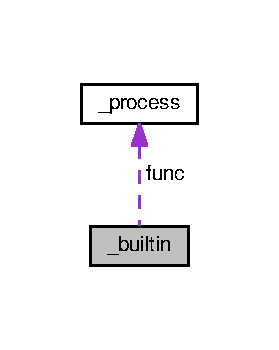
\includegraphics[width=134pt]{struct__builtin__coll__graph}
\end{center}
\end{figure}
\subsection*{Public Attributes}
\begin{DoxyCompactItemize}
\item 
char $\ast$ \hyperlink{struct__builtin_adfb6bdcbe370c381dcb71f91fcc65319}{name}
\begin{DoxyCompactList}\small\item\em The name of the shell builtin. \end{DoxyCompactList}\item 
\hyperlink{job_8h_af6b8d1779250c4d2f3c902dc1aad5a5d}{b\-\_\-func} \hyperlink{struct__builtin_adb30d358f5fb6b16dc124796851e0c48}{func}
\begin{DoxyCompactList}\small\item\em Pointer to the function used to launch the shell builtin. \end{DoxyCompactList}\end{DoxyCompactItemize}


\subsection{Detailed Description}
Maps a shell builtin to a function. 

\begin{DoxyParagraph}{Description}
This structure is used to map a shell builtin to the function that is used to launch it.
\end{DoxyParagraph}
\begin{DoxySeeAlso}{See Also}
\hyperlink{job_8c_a2c5551422426f406568d84844b40acb9}{builtins}, \hyperlink{job_8c_a2c2cfa6591ee05cc5bf0c39f38b9e2ea}{Ash\-\_\-cd()}, \hyperlink{job_8c_a9fa5abe15df71a688905dc7b29a1389f}{Ash\-\_\-exit()}, \hyperlink{job_8c_a8950ee4bf84f8322e0b294d0c448a9e7}{Ash\-\_\-jobs()}, \hyperlink{job_8c_a792fcc9814d020b087911591c5fce10b}{Ash\-\_\-fg()}, \hyperlink{job_8c_a9bc6f26d0ab14359707a0f367f1a6522}{Ash\-\_\-bg()}, \hyperlink{job_8c_a4242d3cdbc0468d774243dc67b330296}{Ash\-\_\-help()}, \hyperlink{job_8h_af6b8d1779250c4d2f3c902dc1aad5a5d}{b\-\_\-func} \hyperlink{job_8c_a723e6648fca47a139cdff5cf4f1bc4bb}{Ash\-\_\-kill()}, \hyperlink{job_8c_a07e5c62e1d5e55012cf188dd32b6cf27}{Ash\-\_\-killall()}, \hyperlink{job_8c_a028aee0dd87474ee61f6c654efe653a2}{is\-\_\-builtin()}, \hyperlink{cle_8c_ab57f2ac63325fc919968e7eb78586965}{command\-\_\-completion()}, \hyperlink{cle_8c_ade079408c61657dc7bbd2142a78e0e8a}{command\-\_\-completion\-\_\-generator()}, and \hyperlink{job_8c_a328634c49391a29ef1d4e86d6bf0ea7e}{execute\-\_\-job()}. 
\end{DoxySeeAlso}


\subsection{Member Data Documentation}
\hypertarget{struct__builtin_adb30d358f5fb6b16dc124796851e0c48}{\index{\-\_\-builtin@{\-\_\-builtin}!func@{func}}
\index{func@{func}!_builtin@{\-\_\-builtin}}
\subsubsection[{func}]{\setlength{\rightskip}{0pt plus 5cm}{\bf b\-\_\-func} \-\_\-builtin\-::func}}\label{struct__builtin_adb30d358f5fb6b16dc124796851e0c48}


Pointer to the function used to launch the shell builtin. 

\begin{DoxyParagraph}{Description}
The pointer to the function used to launch the shell builtin.
\end{DoxyParagraph}
\begin{DoxySeeAlso}{See Also}
\hyperlink{job_8c_a2c5551422426f406568d84844b40acb9}{builtins}, \hyperlink{job_8c_a2c2cfa6591ee05cc5bf0c39f38b9e2ea}{Ash\-\_\-cd()}, \hyperlink{job_8c_a9fa5abe15df71a688905dc7b29a1389f}{Ash\-\_\-exit()}, \hyperlink{job_8c_a8950ee4bf84f8322e0b294d0c448a9e7}{Ash\-\_\-jobs()}, \hyperlink{job_8c_a792fcc9814d020b087911591c5fce10b}{Ash\-\_\-fg()}, \hyperlink{job_8c_a4242d3cdbc0468d774243dc67b330296}{Ash\-\_\-help()}, \hyperlink{job_8c_a723e6648fca47a139cdff5cf4f1bc4bb}{Ash\-\_\-kill()}, \hyperlink{job_8c_a07e5c62e1d5e55012cf188dd32b6cf27}{Ash\-\_\-killall()}, \hyperlink{job_8c_a028aee0dd87474ee61f6c654efe653a2}{is\-\_\-builtin()}, \hyperlink{cle_8c_ab57f2ac63325fc919968e7eb78586965}{command\-\_\-completion()}, \hyperlink{cle_8c_ade079408c61657dc7bbd2142a78e0e8a}{command\-\_\-completion\-\_\-generator()}, \hyperlink{job_8h_af6b8d1779250c4d2f3c902dc1aad5a5d}{b\-\_\-func}, \hyperlink{struct__builtin_adfb6bdcbe370c381dcb71f91fcc65319}{\-\_\-builtin\-::name}, and \hyperlink{job_8c_a328634c49391a29ef1d4e86d6bf0ea7e}{execute\-\_\-job()}. 
\end{DoxySeeAlso}
\hypertarget{struct__builtin_adfb6bdcbe370c381dcb71f91fcc65319}{\index{\-\_\-builtin@{\-\_\-builtin}!name@{name}}
\index{name@{name}!_builtin@{\-\_\-builtin}}
\subsubsection[{name}]{\setlength{\rightskip}{0pt plus 5cm}char$\ast$ \-\_\-builtin\-::name}}\label{struct__builtin_adfb6bdcbe370c381dcb71f91fcc65319}


The name of the shell builtin. 

\begin{DoxyParagraph}{Description}
The name of the shell builtin.
\end{DoxyParagraph}
\begin{DoxySeeAlso}{See Also}
\hyperlink{job_8c_a2c5551422426f406568d84844b40acb9}{builtins}, \hyperlink{job_8c_a2c2cfa6591ee05cc5bf0c39f38b9e2ea}{Ash\-\_\-cd()}, \hyperlink{job_8c_a9fa5abe15df71a688905dc7b29a1389f}{Ash\-\_\-exit()}, \hyperlink{job_8c_a8950ee4bf84f8322e0b294d0c448a9e7}{Ash\-\_\-jobs()}, \hyperlink{job_8c_a792fcc9814d020b087911591c5fce10b}{Ash\-\_\-fg()}, \hyperlink{job_8c_a4242d3cdbc0468d774243dc67b330296}{Ash\-\_\-help()}, \hyperlink{job_8c_a723e6648fca47a139cdff5cf4f1bc4bb}{Ash\-\_\-kill()}, \hyperlink{job_8c_a07e5c62e1d5e55012cf188dd32b6cf27}{Ash\-\_\-killall()}, \hyperlink{job_8c_a028aee0dd87474ee61f6c654efe653a2}{is\-\_\-builtin()}, \hyperlink{cle_8c_ab57f2ac63325fc919968e7eb78586965}{command\-\_\-completion()}, \hyperlink{cle_8c_ade079408c61657dc7bbd2142a78e0e8a}{command\-\_\-completion\-\_\-generator()}, \hyperlink{job_8h_af6b8d1779250c4d2f3c902dc1aad5a5d}{b\-\_\-func}, \hyperlink{struct__builtin_adb30d358f5fb6b16dc124796851e0c48}{\-\_\-builtin\-::func}, and \hyperlink{job_8c_a328634c49391a29ef1d4e86d6bf0ea7e}{execute\-\_\-job()}. 
\end{DoxySeeAlso}


The documentation for this struct was generated from the following file\-:\begin{DoxyCompactItemize}
\item 
src/\hyperlink{job_8h}{job.\-h}\end{DoxyCompactItemize}

\hypertarget{struct__job}{\section{\-\_\-job Struct Reference}
\label{struct__job}\index{\-\_\-job@{\-\_\-job}}
}


Collaboration diagram for \-\_\-job\-:\nopagebreak
\begin{figure}[H]
\begin{center}
\leavevmode
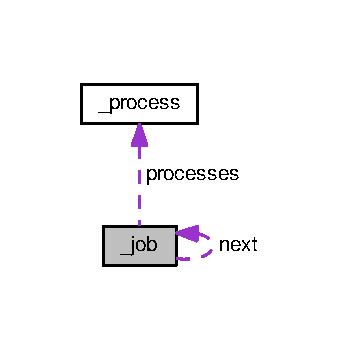
\includegraphics[width=164pt]{struct__job__coll__graph}
\end{center}
\end{figure}
\subsection*{Public Attributes}
\begin{DoxyCompactItemize}
\item 
\hypertarget{struct__job_a9f9d25a2f3ae560112e1d80cec67346c}{struct \hyperlink{struct__job}{\-\_\-job} $\ast$ {\bfseries next}}\label{struct__job_a9f9d25a2f3ae560112e1d80cec67346c}

\item 
\hypertarget{struct__job_a0a95a3cbd137e9af13918781cd735e19}{int {\bfseries id}}\label{struct__job_a0a95a3cbd137e9af13918781cd735e19}

\item 
\hypertarget{struct__job_a640f51218f6cea593af3b726243a1ba5}{\hyperlink{struct__process}{Process} $\ast$ {\bfseries processes} \mbox{[}M\-A\-X\-\_\-\-P\-R\-O\-C\-E\-S\-S\-E\-S\mbox{]}}\label{struct__job_a640f51218f6cea593af3b726243a1ba5}

\item 
\hypertarget{struct__job_ae270f3db5f654203eafbc21b5d7fa903}{int {\bfseries num\-\_\-processes}}\label{struct__job_ae270f3db5f654203eafbc21b5d7fa903}

\item 
\hypertarget{struct__job_a1e2f3ed455c7dad69db4b432ce5a92e5}{pid\-\_\-t {\bfseries pgid}}\label{struct__job_a1e2f3ed455c7dad69db4b432ce5a92e5}

\item 
\hypertarget{struct__job_a8931b8641a21e161f761ac1be42b56c9}{int {\bfseries notified}}\label{struct__job_a8931b8641a21e161f761ac1be42b56c9}

\item 
\hypertarget{struct__job_ad2c040a6b9d36d561301c9db54dfd12d}{struct termios {\bfseries saved\-\_\-tmodes}}\label{struct__job_ad2c040a6b9d36d561301c9db54dfd12d}

\item 
\hypertarget{struct__job_ae70cd46c40d32090f41e666fc01d9e72}{int {\bfseries stdin\-\_\-}}\label{struct__job_ae70cd46c40d32090f41e666fc01d9e72}

\item 
\hypertarget{struct__job_aa1b25162b95a558939e61d036e443e0f}{int {\bfseries stdout\-\_\-}}\label{struct__job_aa1b25162b95a558939e61d036e443e0f}

\item 
\hypertarget{struct__job_a593b516712519cdfa2c2a64bb51b4e07}{int {\bfseries stderr\-\_\-}}\label{struct__job_a593b516712519cdfa2c2a64bb51b4e07}

\item 
\hypertarget{struct__job_a9ee86359ab07771be609532e907b8eb3}{char $\ast$ {\bfseries in\-\_\-file}}\label{struct__job_a9ee86359ab07771be609532e907b8eb3}

\item 
\hypertarget{struct__job_a63d25ff1e6a28380db8d7f732e894a55}{char $\ast$ {\bfseries out\-\_\-file}}\label{struct__job_a63d25ff1e6a28380db8d7f732e894a55}

\item 
\hypertarget{struct__job_ab1f1d871ff9d3892c4cef64d4bc5e8dd}{char $\ast$ {\bfseries err\-\_\-file}}\label{struct__job_ab1f1d871ff9d3892c4cef64d4bc5e8dd}

\item 
\hypertarget{struct__job_abdbdc42c7781216c1dd62f5ada0bc217}{int {\bfseries foreground}}\label{struct__job_abdbdc42c7781216c1dd62f5ada0bc217}

\end{DoxyCompactItemize}


The documentation for this struct was generated from the following file\-:\begin{DoxyCompactItemize}
\item 
src/\hyperlink{job_8h}{job.\-h}\end{DoxyCompactItemize}

\hypertarget{struct__process}{\section{\-\_\-process Struct Reference}
\label{struct__process}\index{\-\_\-process@{\-\_\-process}}
}
\subsection*{Public Attributes}
\begin{DoxyCompactItemize}
\item 
\hypertarget{struct__process_a9bedf3d000c74461921ad68651a3752c}{char $\ast$ {\bfseries argv} \mbox{[}M\-A\-X\-\_\-\-A\-R\-G\-S\mbox{]}}\label{struct__process_a9bedf3d000c74461921ad68651a3752c}

\item 
\hypertarget{struct__process_a101ac531e210400c832cfe4cb05b022f}{int {\bfseries argc}}\label{struct__process_a101ac531e210400c832cfe4cb05b022f}

\item 
\hypertarget{struct__process_aebc44dfe93838e677e88b732390b3721}{pid\-\_\-t {\bfseries pid}}\label{struct__process_aebc44dfe93838e677e88b732390b3721}

\item 
\hypertarget{struct__process_a5b05357cc7128de7d6b6089d6cc4b6b6}{int {\bfseries completed}}\label{struct__process_a5b05357cc7128de7d6b6089d6cc4b6b6}

\item 
\hypertarget{struct__process_a28951ef8d0bf29360fad667dbb12ae77}{int {\bfseries stopped}}\label{struct__process_a28951ef8d0bf29360fad667dbb12ae77}

\item 
\hypertarget{struct__process_a92536d9b184e75911510a19a67049038}{int {\bfseries status}}\label{struct__process_a92536d9b184e75911510a19a67049038}

\end{DoxyCompactItemize}


The documentation for this struct was generated from the following file\-:\begin{DoxyCompactItemize}
\item 
src/\hyperlink{job_8h}{job.\-h}\end{DoxyCompactItemize}

\hypertarget{structyy__buffer__state}{\section{yy\-\_\-buffer\-\_\-state Struct Reference}
\label{structyy__buffer__state}\index{yy\-\_\-buffer\-\_\-state@{yy\-\_\-buffer\-\_\-state}}
}
\subsection*{Public Attributes}
\begin{DoxyCompactItemize}
\item 
\hypertarget{structyy__buffer__state_a4843d1422e3276b636d475a3095bd948}{F\-I\-L\-E $\ast$ {\bfseries yy\-\_\-input\-\_\-file}}\label{structyy__buffer__state_a4843d1422e3276b636d475a3095bd948}

\item 
\hypertarget{structyy__buffer__state_ad7b8df8d8a4688e57b0b8d3ca75adc85}{char $\ast$ {\bfseries yy\-\_\-ch\-\_\-buf}}\label{structyy__buffer__state_ad7b8df8d8a4688e57b0b8d3ca75adc85}

\item 
\hypertarget{structyy__buffer__state_a58aa927f098b99d99e75da80f9b681ef}{char $\ast$ {\bfseries yy\-\_\-buf\-\_\-pos}}\label{structyy__buffer__state_a58aa927f098b99d99e75da80f9b681ef}

\item 
\hypertarget{structyy__buffer__state_a48302f5f3477a9c78bbddf56d356ef54}{yy\-\_\-size\-\_\-t {\bfseries yy\-\_\-buf\-\_\-size}}\label{structyy__buffer__state_a48302f5f3477a9c78bbddf56d356ef54}

\item 
\hypertarget{structyy__buffer__state_a06406208824817acfec2183b79080945}{int {\bfseries yy\-\_\-n\-\_\-chars}}\label{structyy__buffer__state_a06406208824817acfec2183b79080945}

\item 
\hypertarget{structyy__buffer__state_a80ce2431c70dc4f89ced487f18449465}{int {\bfseries yy\-\_\-is\-\_\-our\-\_\-buffer}}\label{structyy__buffer__state_a80ce2431c70dc4f89ced487f18449465}

\item 
\hypertarget{structyy__buffer__state_abf5c70eea75581b58c0ee7bd31b14490}{int {\bfseries yy\-\_\-is\-\_\-interactive}}\label{structyy__buffer__state_abf5c70eea75581b58c0ee7bd31b14490}

\item 
\hypertarget{structyy__buffer__state_a9d60c60af6e1a6f69de16871fd64f85f}{int {\bfseries yy\-\_\-at\-\_\-bol}}\label{structyy__buffer__state_a9d60c60af6e1a6f69de16871fd64f85f}

\item 
\hypertarget{structyy__buffer__state_a63d2afbb1d79a3fc63df9e12626f827d}{int {\bfseries yy\-\_\-fill\-\_\-buffer}}\label{structyy__buffer__state_a63d2afbb1d79a3fc63df9e12626f827d}

\item 
\hypertarget{structyy__buffer__state_a70fd925d37a2f0454fbd0def675d106c}{int {\bfseries yy\-\_\-buffer\-\_\-status}}\label{structyy__buffer__state_a70fd925d37a2f0454fbd0def675d106c}

\end{DoxyCompactItemize}


The documentation for this struct was generated from the following file\-:\begin{DoxyCompactItemize}
\item 
src/lex.\-yy.\-c\end{DoxyCompactItemize}

\hypertarget{unionyy__parse__stype}{\section{yy\-\_\-parse\-\_\-stype Union Reference}
\label{unionyy__parse__stype}\index{yy\-\_\-parse\-\_\-stype@{yy\-\_\-parse\-\_\-stype}}
}
\subsection*{Public Attributes}
\begin{DoxyCompactItemize}
\item 
\hypertarget{unionyy__parse__stype_ab41b871d18b9bfd3700d3fdebb3c65c6}{char $\ast$ {\bfseries str}}\label{unionyy__parse__stype_ab41b871d18b9bfd3700d3fdebb3c65c6}

\item 
\hypertarget{unionyy__parse__stype_a5024e073eb15bd6c3c21760a50e7df8e}{int {\bfseries i}}\label{unionyy__parse__stype_a5024e073eb15bd6c3c21760a50e7df8e}

\end{DoxyCompactItemize}


The documentation for this union was generated from the following files\-:\begin{DoxyCompactItemize}
\item 
src/y.\-tab.\-c\item 
src/y.\-tab.\-h\end{DoxyCompactItemize}

\chapter{File Documentation}
\hypertarget{cle_8c}{\section{src/cle.c File Reference}
\label{cle_8c}\index{src/cle.\-c@{src/cle.\-c}}
}


Contains the code for the command line editing sub system.  


{\ttfamily \#include $<$stdio.\-h$>$}\\*
{\ttfamily \#include $<$readline/readline.\-h$>$}\\*
{\ttfamily \#include $<$readline/history.\-h$>$}\\*
{\ttfamily \#include $<$stdlib.\-h$>$}\\*
{\ttfamily \#include $<$unistd.\-h$>$}\\*
{\ttfamily \#include $<$string.\-h$>$}\\*
{\ttfamily \#include \char`\"{}cle.\-h\char`\"{}}\\*
{\ttfamily \#include \char`\"{}err.\-h\char`\"{}}\\*
{\ttfamily \#include \char`\"{}job.\-h\char`\"{}}\\*
{\ttfamily \#include $<$limits.\-h$>$}\\*
Include dependency graph for cle.\-c\-:\nopagebreak
\begin{figure}[H]
\begin{center}
\leavevmode
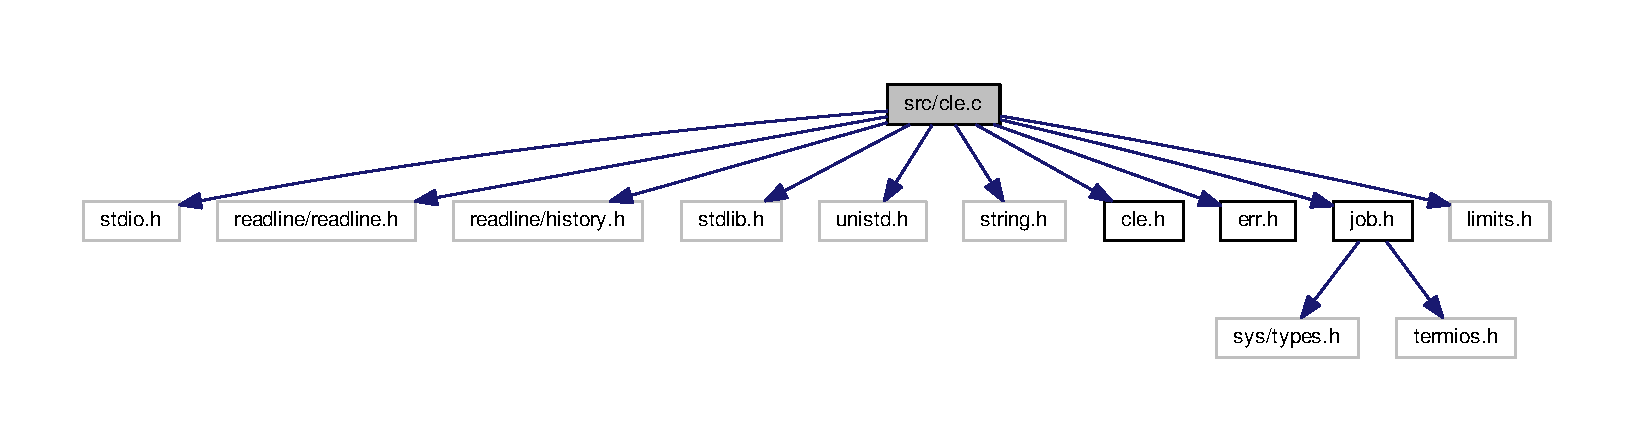
\includegraphics[width=350pt]{cle_8c__incl}
\end{center}
\end{figure}
\subsection*{Functions}
\begin{DoxyCompactItemize}
\item 
int \hyperlink{cle_8c_a31a3775714cbd1b923fa3ec2c5c7fd48}{remove\-\_\-lines\-\_\-from\-\_\-file} (char $\ast$file\-\_\-name, int start\-\_\-line, int line\-\_\-count)
\begin{DoxyCompactList}\small\item\em Removes lines from a file. \end{DoxyCompactList}\item 
int \hyperlink{cle_8c_a327aaeef5e5ada52f0a64d0be178bb30}{invert\-\_\-case\-\_\-in\-\_\-region} (int count, int key)
\begin{DoxyCompactList}\small\item\em Inverts the case of characters in a region of the current line buffer of {\itshape readline} . \end{DoxyCompactList}\item 
int \hyperlink{cle_8c_a74b72242dbf240d23501bb34bfdc4fea}{count\-\_\-lines\-\_\-in\-\_\-file} (const char $\ast$file\-\_\-name)
\begin{DoxyCompactList}\small\item\em Counts the number of lines in a file. \end{DoxyCompactList}\item 
char $\ast$$\ast$ \hyperlink{cle_8c_ab57f2ac63325fc919968e7eb78586965}{command\-\_\-completion} (const char $\ast$partial\-\_\-text, int start, int end)
\begin{DoxyCompactList}\small\item\em Registred function to perform command completion. \end{DoxyCompactList}\item 
char $\ast$ \hyperlink{cle_8c_ade079408c61657dc7bbd2142a78e0e8a}{command\-\_\-completion\-\_\-generator} (const char $\ast$partial\-\_\-text, int state)
\begin{DoxyCompactList}\small\item\em Generation function used for command completion. \end{DoxyCompactList}\item 
int \hyperlink{cle_8c_a8a75575085afe93be976c3d116ed8231}{toggle\-\_\-editing\-\_\-mode} (int count, int key)
\begin{DoxyCompactList}\small\item\em Toggles {\itshape readline} 's editing mode. \end{DoxyCompactList}\item 
int \hyperlink{cle_8c_acbd58e7ffbca9f6d8d7494a053414e49}{initialize\-\_\-history} ()
\begin{DoxyCompactList}\small\item\em Initializes the shell's command history facilities. \end{DoxyCompactList}\item 
int \hyperlink{cle_8c_a371915dea0605bdd469053706d93951d}{initialize\-\_\-readline} ()
\begin{DoxyCompactList}\small\item\em Initializes the shell's commmandline editing facilities. \end{DoxyCompactList}\item 
char $\ast$ \hyperlink{cle_8c_a19bb8493640e845196c4d763f4109b67}{\-\_\-readline} (const char $\ast$prompt\-\_\-string)
\begin{DoxyCompactList}\small\item\em Calls {\itshape readline()} to read input and manages the shell's command history. \end{DoxyCompactList}\end{DoxyCompactItemize}
\subsection*{Variables}
\begin{DoxyCompactItemize}
\item 
char $\ast$ \hyperlink{cle_8c_a48b5776fb79c56d2584cfa6f109e8f22}{line\-\_\-buffer} = N\-U\-L\-L
\begin{DoxyCompactList}\small\item\em Stores the address of the last {\itshape readline} buffer. \end{DoxyCompactList}\item 
char \hyperlink{cle_8c_a4a65daaf4e44aa02a8fac3ed42ec9f68}{H\-I\-S\-T\-O\-R\-Y\-\_\-\-F\-I\-L\-E} \mbox{[}P\-A\-T\-H\-\_\-\-M\-A\-X\mbox{]}
\begin{DoxyCompactList}\small\item\em Stores the path of the command history file. \end{DoxyCompactList}\item 
char \hyperlink{cle_8c_a2b3f51fec8189b0ed52c3a29b4d7614e}{I\-N\-P\-U\-T\-R\-C\-\_\-\-F\-I\-L\-E} \mbox{[}P\-A\-T\-H\-\_\-\-M\-A\-X\mbox{]}
\begin{DoxyCompactList}\small\item\em Stores the path of the {\itshape readline} input file. \end{DoxyCompactList}\item 
int \hyperlink{cle_8c_a26c966f13355ca7e2a3fb8a6c3fb51c0}{N\-U\-M\-\_\-\-E\-N\-T\-R\-I\-E\-S\-\_\-\-H\-I\-S\-T\-O\-R\-Y\-\_\-\-F\-I\-L\-E}
\begin{DoxyCompactList}\small\item\em Stores the current number of entries in the command history file. \end{DoxyCompactList}\item 
int \hyperlink{cle_8c_a11b4616ee9e2b6f719a050b70a70b59d}{M\-A\-X\-\_\-\-N\-U\-M\-\_\-\-E\-N\-T\-R\-I\-E\-S\-\_\-\-H\-I\-S\-T\-O\-R\-Y\-\_\-\-F\-I\-L\-E} = 500
\begin{DoxyCompactList}\small\item\em Stores the maximum number of entries allowed in the command history file. \end{DoxyCompactList}\item 
\hyperlink{job_8h_a165885ac9a829b970ba29594fec5acd7}{Builtin} \hyperlink{cle_8c_a2c5551422426f406568d84844b40acb9}{builtins} \mbox{[}$\,$\mbox{]}
\begin{DoxyCompactList}\small\item\em List of shell builtins an associated function. \end{DoxyCompactList}\end{DoxyCompactItemize}


\subsection{Detailed Description}
Contains the code for the command line editing sub system. \begin{DoxyAuthor}{Author}
Joe Nathan Abellard \{\href{https://github.com/joenatech7}{\tt https\-://github.\-com/joenatech7}\}
\end{DoxyAuthor}
\begin{DoxyDate}{Date}
September 1, 2017 
\end{DoxyDate}
\begin{DoxyParagraph}{Description}
This file contains contains the code for the command line editing sub subsystem.
\end{DoxyParagraph}
\begin{DoxySeeAlso}{See Also}
\hyperlink{cle_8h}{cle.\-h} 
\end{DoxySeeAlso}


\subsection{Function Documentation}
\hypertarget{cle_8c_a19bb8493640e845196c4d763f4109b67}{\index{cle.\-c@{cle.\-c}!\-\_\-readline@{\-\_\-readline}}
\index{\-\_\-readline@{\-\_\-readline}!cle.c@{cle.\-c}}
\subsubsection[{\-\_\-readline}]{\setlength{\rightskip}{0pt plus 5cm}char$\ast$ \-\_\-readline (
\begin{DoxyParamCaption}
\item[{const char $\ast$}]{}
\end{DoxyParamCaption}
)}}\label{cle_8c_a19bb8493640e845196c4d763f4109b67}


Calls {\itshape readline()} to read input and manages the shell's command history. 

\begin{DoxyParagraph}{Description}
This function is used to call @ readline() to read input from the shell prompt, and to manage the shell's command history. It does the following\-: \begin{DoxyItemize}
\item Calls \hyperlink{err_8h_a40bd4201ea3cf1b6f8e7fef01362bf67}{sfree} to de-\/allocate the memory block of the last line buffer returned by (), if nessasary. This buffer is pointed to by \hyperlink{cle_8c_a48b5776fb79c56d2584cfa6f109e8f22}{line\-\_\-buffer}. \hyperlink{cle_8c_a48b5776fb79c56d2584cfa6f109e8f22}{line\-\_\-buffer} is aliased by \hyperlink{main_8c_ae8d7cb95bc48828d10bf3c7a31680ce2}{pipeline\-\_\-list} in \hyperlink{main_8c_af783a9705a73559f4b17ec991bc11f1e}{input\-\_\-loop()}. To avoid a possible double free exeption, \hyperlink{main_8c_ae8d7cb95bc48828d10bf3c7a31680ce2}{pipeline\-\_\-list} should never be used to free the {\itshape readline} buffer. \item Calls {\itshape readline()} to read input, and assigns the location of the {\itshape readline} buffer to \hyperlink{cle_8c_a48b5776fb79c56d2584cfa6f109e8f22}{line\-\_\-buffer}. \item If the {\itshape readline} buffer is not empty, then add the line read to the history list and to the history file (\hyperlink{cle_8c_a4a65daaf4e44aa02a8fac3ed42ec9f68}{H\-I\-S\-T\-O\-R\-Y\-\_\-\-F\-I\-L\-E}). If insertion of the new entry would result in the history file having more than \hyperlink{cle_8c_a11b4616ee9e2b6f719a050b70a70b59d}{M\-A\-X\-\_\-\-N\-U\-M\-\_\-\-E\-N\-T\-R\-I\-E\-S\-\_\-\-H\-I\-S\-T\-O\-R\-Y\-\_\-\-F\-I\-L\-E}, or that the history file already contains more than M\-A\-X\-\_\-\-N\-U\-M\-\_\-\-E\-N\-T\-R\-I\-E\-S\-\_\-\-H\-I\-S\-T\-O\-R\-Y\-\_\-\-F\-I\-L\-E, then the function invokes removed\-\_\-lines\-\_\-from\-\_\-file() to remove lines from the history file before performing the insertion.\end{DoxyItemize}

\end{DoxyParagraph}

\begin{DoxyParams}{Parameters}
{\em promt\-\_\-string} & The prompt string that is displayed on the terminal.\\
\hline
\end{DoxyParams}
\begin{DoxyReturn}{Returns}
Returns \hyperlink{cle_8c_a48b5776fb79c56d2584cfa6f109e8f22}{line\-\_\-buffer}.
\end{DoxyReturn}
\begin{DoxySeeAlso}{See Also}
\hyperlink{err_8h_a40bd4201ea3cf1b6f8e7fef01362bf67}{sfree}, \hyperlink{cle_8c_a48b5776fb79c56d2584cfa6f109e8f22}{line\-\_\-buffer}, readline(), \hyperlink{cle_8c_a11b4616ee9e2b6f719a050b70a70b59d}{M\-A\-X\-\_\-\-N\-U\-M\-\_\-\-E\-N\-T\-R\-I\-E\-S\-\_\-\-H\-I\-S\-T\-O\-R\-Y\-\_\-\-F\-I\-L\-E}, \hyperlink{cle_8c_a26c966f13355ca7e2a3fb8a6c3fb51c0}{N\-U\-M\-\_\-\-E\-N\-T\-R\-I\-E\-S\-\_\-\-H\-I\-S\-T\-O\-R\-Y\-\_\-\-F\-I\-L\-E}, \hyperlink{cle_8h_a31a3775714cbd1b923fa3ec2c5c7fd48}{remove\-\_\-lines\-\_\-from\-\_\-file()}, \hyperlink{main_8c_ae8d7cb95bc48828d10bf3c7a31680ce2}{pipeline\-\_\-list}, and \hyperlink{main_8c_af783a9705a73559f4b17ec991bc11f1e}{input\-\_\-loop()}. 
\end{DoxySeeAlso}


Here is the call graph for this function\-:\nopagebreak
\begin{figure}[H]
\begin{center}
\leavevmode
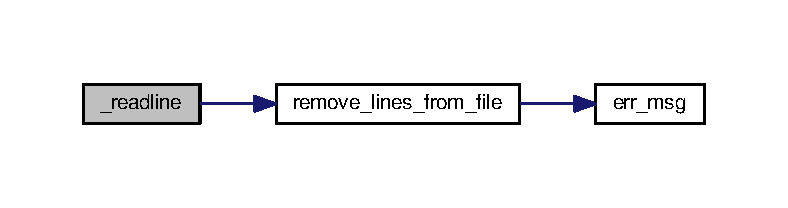
\includegraphics[width=350pt]{cle_8c_a19bb8493640e845196c4d763f4109b67_cgraph}
\end{center}
\end{figure}




Here is the caller graph for this function\-:\nopagebreak
\begin{figure}[H]
\begin{center}
\leavevmode
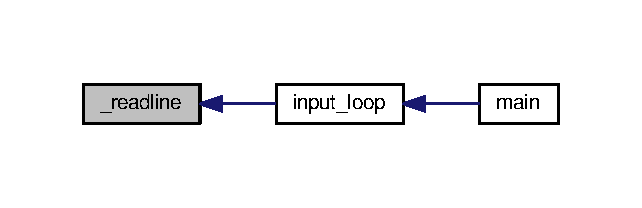
\includegraphics[width=308pt]{cle_8c_a19bb8493640e845196c4d763f4109b67_icgraph}
\end{center}
\end{figure}


\hypertarget{cle_8c_ab57f2ac63325fc919968e7eb78586965}{\index{cle.\-c@{cle.\-c}!command\-\_\-completion@{command\-\_\-completion}}
\index{command\-\_\-completion@{command\-\_\-completion}!cle.c@{cle.\-c}}
\subsubsection[{command\-\_\-completion}]{\setlength{\rightskip}{0pt plus 5cm}char$\ast$$\ast$ command\-\_\-completion (
\begin{DoxyParamCaption}
\item[{const char $\ast$}]{, }
\item[{int}]{, }
\item[{int}]{}
\end{DoxyParamCaption}
)}}\label{cle_8c_ab57f2ac63325fc919968e7eb78586965}


Registred function to perform command completion. 

\begin{DoxyParagraph}{Description}
This function is assigned to {\itshape readline's} {\itshape rl\-\_\-attempted\-\_\-completion} variable. Consequently, when the tab key is pressed on the command line, it is invoked to perform command completion on a partial text. It uses {\itshape readline's} {\itshape rl\-\_\-completion\-\_\-matches} function with the \hyperlink{cle_8h_af9de2a3a174e2493e7f3e168949bf84f}{command\-\_\-completion\-\_\-generator()} genarator function to find possible completions for the partial text in the list of commands in the \hyperlink{job_8c_a2c5551422426f406568d84844b40acb9}{builtins} array
\end{DoxyParagraph}

\begin{DoxyParams}{Parameters}
{\em partial\-\_\-text} & The partial text to be completed.\\
\hline
{\em start} & The starting position of {\itshape partial\-\_\-text} in {\itshape readline's} line buffer.\\
\hline
{\em end} & The ending position of {\itshape partial\-\_\-text} in {\itshape readline's} line buffer.\\
\hline
\end{DoxyParams}
\begin{DoxyReturn}{Returns}
Returns an array of pointers to strings. Three outcomes are possible \-: \begin{DoxyItemize}
\item No possible completions found. In that case, the first element of the array points to N\-U\-L\-L. \item One possible completion was found. In that case, the first element of the array points to the possible completion string, and the second element points to N\-U\-L\-L. \item {\itshape n$>$=2} possible completion were found. In that case, the first {\itshape n} elements of the array point to the {\itshape n} possible completion strings, and the {\itshape }(n + 1)th element of the array points to N\-U\-L\-L.\end{DoxyItemize}

\end{DoxyReturn}
\begin{DoxySeeAlso}{See Also}
{\itshape readline} , \hyperlink{cle_8h_a371915dea0605bdd469053706d93951d}{initialize\-\_\-readline()}, command\-\_\-completion\-\_\-genarator(), and \hyperlink{job_8c_a2c5551422426f406568d84844b40acb9}{builtins}. 
\end{DoxySeeAlso}


Here is the call graph for this function\-:\nopagebreak
\begin{figure}[H]
\begin{center}
\leavevmode
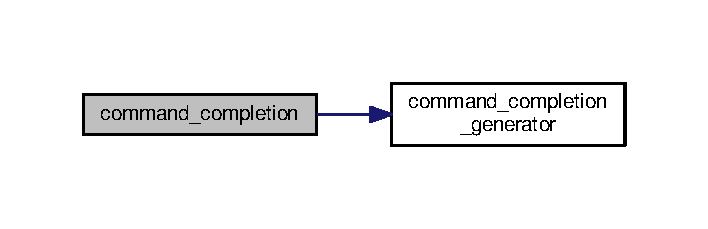
\includegraphics[width=340pt]{cle_8c_ab57f2ac63325fc919968e7eb78586965_cgraph}
\end{center}
\end{figure}




Here is the caller graph for this function\-:\nopagebreak
\begin{figure}[H]
\begin{center}
\leavevmode
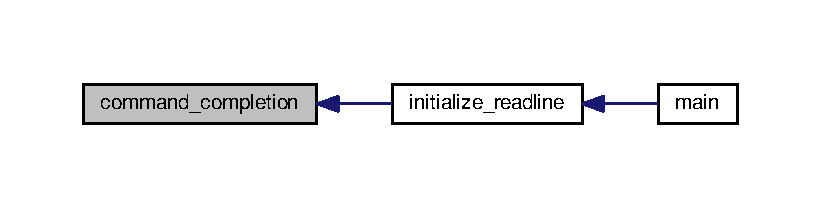
\includegraphics[width=350pt]{cle_8c_ab57f2ac63325fc919968e7eb78586965_icgraph}
\end{center}
\end{figure}


\hypertarget{cle_8c_ade079408c61657dc7bbd2142a78e0e8a}{\index{cle.\-c@{cle.\-c}!command\-\_\-completion\-\_\-generator@{command\-\_\-completion\-\_\-generator}}
\index{command\-\_\-completion\-\_\-generator@{command\-\_\-completion\-\_\-generator}!cle.c@{cle.\-c}}
\subsubsection[{command\-\_\-completion\-\_\-generator}]{\setlength{\rightskip}{0pt plus 5cm}char$\ast$ command\-\_\-completion\-\_\-generator (
\begin{DoxyParamCaption}
\item[{const char $\ast$}]{, }
\item[{int}]{}
\end{DoxyParamCaption}
)}}\label{cle_8c_ade079408c61657dc7bbd2142a78e0e8a}


Generation function used for command completion. 

\begin{DoxyParagraph}{Description}
This generation function is used by \hyperlink{cle_8h_a839745638ece1570d3c7792dfa182ae7}{command\-\_\-completion()} to find possible command completions in the \hyperlink{job_8c_a2c5551422426f406568d84844b40acb9}{builtins} array.
\end{DoxyParagraph}

\begin{DoxyParams}{Parameters}
{\em partial\-\_\-text} & The partial text to be completed.\\
\hline
{\em state} & The first time the function is called, state is {\itshape 0}. When state is zero, the function initialize some static variables.\\
\hline
\end{DoxyParams}
\begin{DoxyReturn}{Returns}
If a possible completion for {\itshape partial\-\_\-text} is found in the \hyperlink{job_8c_a2c5551422426f406568d84844b40acb9}{builtins} array, the function returns a copy to the completion string. Otherwise, it returns N\-U\-L\-L.
\end{DoxyReturn}
\begin{DoxySeeAlso}{See Also}
\hyperlink{cle_8h_a839745638ece1570d3c7792dfa182ae7}{command\-\_\-completion()}, \hyperlink{job_8c_a2c5551422426f406568d84844b40acb9}{builtins}, and {\itshape readline} . 
\end{DoxySeeAlso}


Here is the caller graph for this function\-:\nopagebreak
\begin{figure}[H]
\begin{center}
\leavevmode
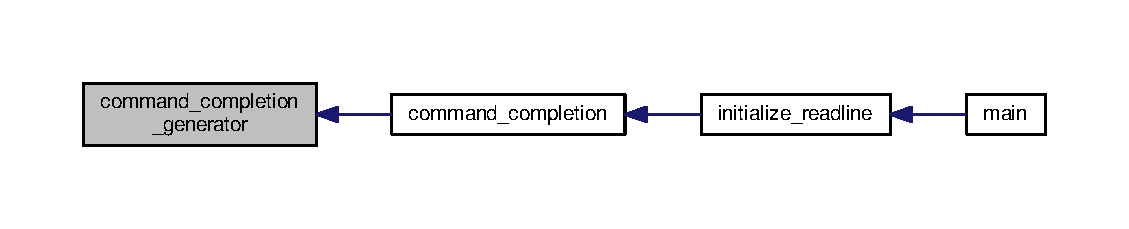
\includegraphics[width=350pt]{cle_8c_ade079408c61657dc7bbd2142a78e0e8a_icgraph}
\end{center}
\end{figure}


\hypertarget{cle_8c_a74b72242dbf240d23501bb34bfdc4fea}{\index{cle.\-c@{cle.\-c}!count\-\_\-lines\-\_\-in\-\_\-file@{count\-\_\-lines\-\_\-in\-\_\-file}}
\index{count\-\_\-lines\-\_\-in\-\_\-file@{count\-\_\-lines\-\_\-in\-\_\-file}!cle.c@{cle.\-c}}
\subsubsection[{count\-\_\-lines\-\_\-in\-\_\-file}]{\setlength{\rightskip}{0pt plus 5cm}int count\-\_\-lines\-\_\-in\-\_\-file (
\begin{DoxyParamCaption}
\item[{const char $\ast$}]{}
\end{DoxyParamCaption}
)}}\label{cle_8c_a74b72242dbf240d23501bb34bfdc4fea}


Counts the number of lines in a file. 

\begin{DoxyParagraph}{Description}
This function is used to count the number of lines in a file.
\end{DoxyParagraph}

\begin{DoxyParams}{Parameters}
{\em file\-\_\-name} & The pathname of the file.\\
\hline
\end{DoxyParams}
\begin{DoxyReturn}{Returns}
Returns {\itshape -\/1} on failure, or the number of lines in the file on success. Possible reasons for failure are as follows\-: \begin{DoxyItemize}
\item The specified file could not be opened.\end{DoxyItemize}

\end{DoxyReturn}
\begin{DoxySeeAlso}{See Also}
\hyperlink{cle_8h_a31a3775714cbd1b923fa3ec2c5c7fd48}{remove\-\_\-lines\-\_\-from\-\_\-file()}, \hyperlink{cle_8h_acbd58e7ffbca9f6d8d7494a053414e49}{initialize\-\_\-history()}, \hyperlink{cle_8c_a4a65daaf4e44aa02a8fac3ed42ec9f68}{H\-I\-S\-T\-O\-R\-Y\-\_\-\-F\-I\-L\-E}, {\itshape fopen()}, {\itshape getc()}, {\itshape fclose()}, and \hyperlink{cle_8c_a26c966f13355ca7e2a3fb8a6c3fb51c0}{N\-U\-M\-\_\-\-E\-N\-T\-R\-I\-E\-S\-\_\-\-H\-I\-S\-T\-O\-R\-Y\-\_\-\-F\-I\-L\-E}. 
\end{DoxySeeAlso}


Here is the caller graph for this function\-:\nopagebreak
\begin{figure}[H]
\begin{center}
\leavevmode
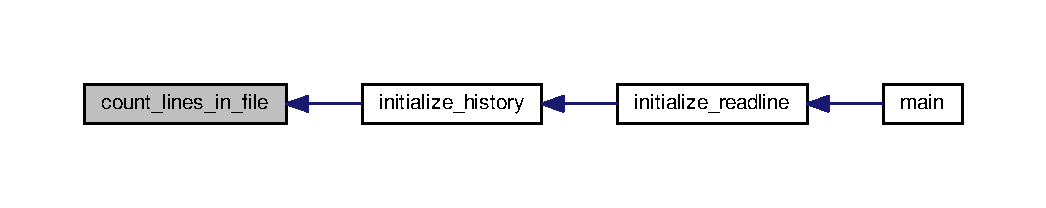
\includegraphics[width=350pt]{cle_8c_a74b72242dbf240d23501bb34bfdc4fea_icgraph}
\end{center}
\end{figure}


\hypertarget{cle_8c_acbd58e7ffbca9f6d8d7494a053414e49}{\index{cle.\-c@{cle.\-c}!initialize\-\_\-history@{initialize\-\_\-history}}
\index{initialize\-\_\-history@{initialize\-\_\-history}!cle.c@{cle.\-c}}
\subsubsection[{initialize\-\_\-history}]{\setlength{\rightskip}{0pt plus 5cm}int initialize\-\_\-history (
\begin{DoxyParamCaption}
{}
\end{DoxyParamCaption}
)}}\label{cle_8c_acbd58e7ffbca9f6d8d7494a053414e49}


Initializes the shell's command history facilities. 

\begin{DoxyParagraph}{Description}
This function is used to initialize the shell's command history facilities. It does the following \-: \begin{DoxyItemize}
\item Calls using\-\_\-history() to make history facilities available. \item Sets the maximum number of enties in the shell's history list to \hyperlink{cle_8c_a11b4616ee9e2b6f719a050b70a70b59d}{M\-A\-X\-\_\-\-N\-U\-M\-\_\-\-E\-N\-T\-R\-I\-E\-S\-\_\-\-H\-I\-S\-T\-O\-R\-Y\-\_\-\-F\-I\-L\-E}. \item Obtains the pathname of the shell's history file and stores the result in \hyperlink{cle_8c_a4a65daaf4e44aa02a8fac3ed42ec9f68}{H\-I\-S\-T\-O\-R\-Y\-\_\-\-F\-I\-L\-E}. \item Obtains the number of lines in the shell's history file (\hyperlink{cle_8c_a4a65daaf4e44aa02a8fac3ed42ec9f68}{H\-I\-S\-T\-O\-R\-Y\-\_\-\-F\-I\-L\-E}) via \hyperlink{cle_8h_a1e9cca6339e637e5dae988a369265b24}{count\-\_\-lines\-\_\-in\-\_\-file()} , and assigns the value to \hyperlink{cle_8c_a26c966f13355ca7e2a3fb8a6c3fb51c0}{N\-U\-M\-\_\-\-E\-N\-T\-R\-I\-E\-S\-\_\-\-H\-I\-S\-T\-O\-R\-Y\-\_\-\-F\-I\-L\-E}. \item Reads history from the history file (\hyperlink{cle_8c_a4a65daaf4e44aa02a8fac3ed42ec9f68}{H\-I\-S\-T\-O\-R\-Y\-\_\-\-F\-I\-L\-E}) into the shell's history list. \item Disables the recording of timestamps for history entries.\end{DoxyItemize}

\end{DoxyParagraph}
\begin{DoxyReturn}{Returns}
Returns {\itshape void}.
\end{DoxyReturn}
\begin{DoxySeeAlso}{See Also}
and \hyperlink{cle_8h_a371915dea0605bdd469053706d93951d}{initialize\-\_\-readline()}. \hyperlink{cle_8c_a11b4616ee9e2b6f719a050b70a70b59d}{M\-A\-X\-\_\-\-N\-U\-M\-\_\-\-E\-N\-T\-R\-I\-E\-S\-\_\-\-H\-I\-S\-T\-O\-R\-Y\-\_\-\-F\-I\-L\-E}, \hyperlink{cle_8c_a4a65daaf4e44aa02a8fac3ed42ec9f68}{H\-I\-S\-T\-O\-R\-Y\-\_\-\-F\-I\-L\-E}, \hyperlink{cle_8c_a26c966f13355ca7e2a3fb8a6c3fb51c0}{N\-U\-M\-\_\-\-E\-N\-T\-R\-I\-E\-S\-\_\-\-H\-I\-S\-T\-O\-R\-Y\-\_\-\-F\-I\-L\-E}, \hyperlink{cle_8h_a1e9cca6339e637e5dae988a369265b24}{count\-\_\-lines\-\_\-in\-\_\-file()}, 
\end{DoxySeeAlso}


Here is the call graph for this function\-:\nopagebreak
\begin{figure}[H]
\begin{center}
\leavevmode
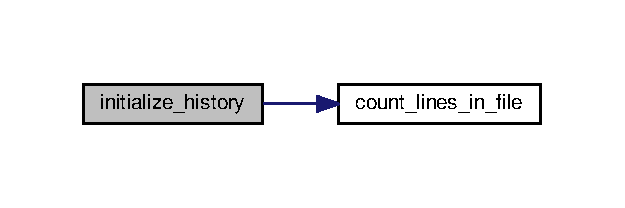
\includegraphics[width=300pt]{cle_8c_acbd58e7ffbca9f6d8d7494a053414e49_cgraph}
\end{center}
\end{figure}




Here is the caller graph for this function\-:\nopagebreak
\begin{figure}[H]
\begin{center}
\leavevmode
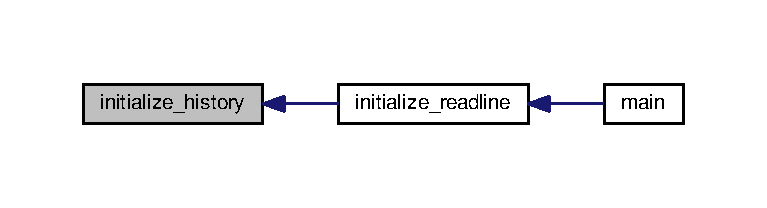
\includegraphics[width=350pt]{cle_8c_acbd58e7ffbca9f6d8d7494a053414e49_icgraph}
\end{center}
\end{figure}


\hypertarget{cle_8c_a371915dea0605bdd469053706d93951d}{\index{cle.\-c@{cle.\-c}!initialize\-\_\-readline@{initialize\-\_\-readline}}
\index{initialize\-\_\-readline@{initialize\-\_\-readline}!cle.c@{cle.\-c}}
\subsubsection[{initialize\-\_\-readline}]{\setlength{\rightskip}{0pt plus 5cm}int initialize\-\_\-readline (
\begin{DoxyParamCaption}
{}
\end{DoxyParamCaption}
)}}\label{cle_8c_a371915dea0605bdd469053706d93951d}


Initializes the shell's commmandline editing facilities. 

\begin{DoxyParagraph}{Description}
This function is used to initialize the shell's commandline editing facilities. It does the following \-: \begin{DoxyItemize}
\item Calls \hyperlink{cle_8h_acbd58e7ffbca9f6d8d7494a053414e49}{initialize\-\_\-history()} to initialize the shell's command history facilities. \item Registers the shell's command completion function (\hyperlink{cle_8h_a839745638ece1570d3c7792dfa182ae7}{command\-\_\-completion()}). \item Registers custom binable functions (\hyperlink{cle_8h_a327aaeef5e5ada52f0a64d0be178bb30}{invert\-\_\-case\-\_\-in\-\_\-region()}, and \hyperlink{cle_8h_a8a75575085afe93be976c3d116ed8231}{toggle\-\_\-editing\-\_\-mode()}). \item Obtains the path of {\itshape readline} 's {\itshape inputrc} file and assign the value to \hyperlink{cle_8c_a2b3f51fec8189b0ed52c3a29b4d7614e}{I\-N\-P\-U\-T\-R\-C\-\_\-\-F\-I\-L\-E}. \item Sets the I\-N\-P\-U\-T\-R\-C environment variable. \item Reads settings from the input file (\hyperlink{cle_8c_a2b3f51fec8189b0ed52c3a29b4d7614e}{I\-N\-P\-U\-T\-R\-C\-\_\-\-F\-I\-L\-E}).\end{DoxyItemize}

\end{DoxyParagraph}
\begin{DoxyReturn}{Returns}
Returns {\itshape -\/1} on failure, or {\itshape 0} on success.
\end{DoxyReturn}
\begin{DoxySeeAlso}{See Also}
\hyperlink{cle_8h_acbd58e7ffbca9f6d8d7494a053414e49}{initialize\-\_\-history()}, \hyperlink{cle_8h_a839745638ece1570d3c7792dfa182ae7}{command\-\_\-completion()}, \hyperlink{cle_8h_a327aaeef5e5ada52f0a64d0be178bb30}{invert\-\_\-case\-\_\-in\-\_\-region()}, \hyperlink{cle_8h_a8a75575085afe93be976c3d116ed8231}{toggle\-\_\-editing\-\_\-mode()}, \hyperlink{cle_8c_a2b3f51fec8189b0ed52c3a29b4d7614e}{I\-N\-P\-U\-T\-R\-C\-\_\-\-F\-I\-L\-E}, {\itshape readline} , {\itshape inputrc}, and (). 
\end{DoxySeeAlso}


Here is the call graph for this function\-:\nopagebreak
\begin{figure}[H]
\begin{center}
\leavevmode
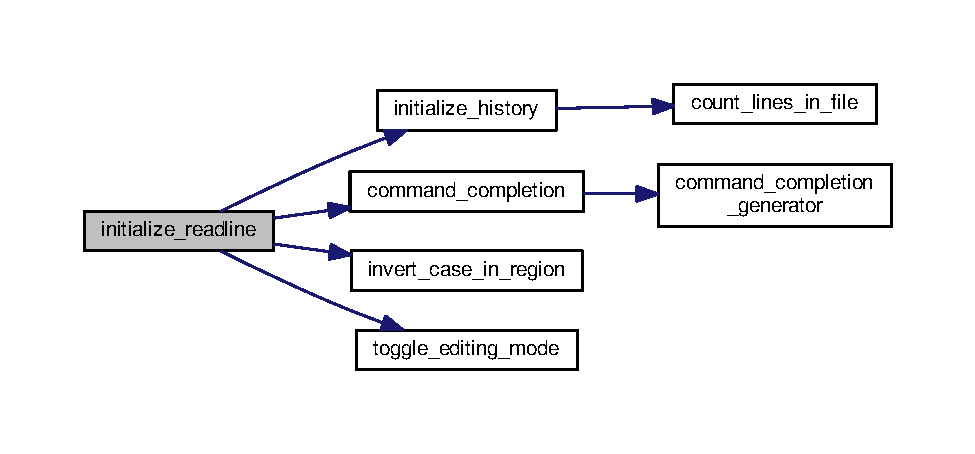
\includegraphics[width=350pt]{cle_8c_a371915dea0605bdd469053706d93951d_cgraph}
\end{center}
\end{figure}




Here is the caller graph for this function\-:\nopagebreak
\begin{figure}[H]
\begin{center}
\leavevmode
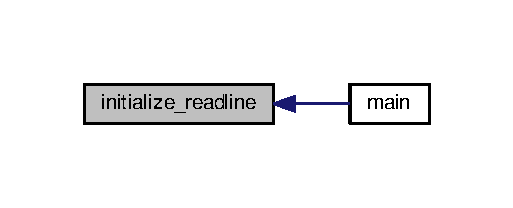
\includegraphics[width=246pt]{cle_8c_a371915dea0605bdd469053706d93951d_icgraph}
\end{center}
\end{figure}


\hypertarget{cle_8c_a327aaeef5e5ada52f0a64d0be178bb30}{\index{cle.\-c@{cle.\-c}!invert\-\_\-case\-\_\-in\-\_\-region@{invert\-\_\-case\-\_\-in\-\_\-region}}
\index{invert\-\_\-case\-\_\-in\-\_\-region@{invert\-\_\-case\-\_\-in\-\_\-region}!cle.c@{cle.\-c}}
\subsubsection[{invert\-\_\-case\-\_\-in\-\_\-region}]{\setlength{\rightskip}{0pt plus 5cm}int invert\-\_\-case\-\_\-in\-\_\-region (
\begin{DoxyParamCaption}
\item[{int}]{count, }
\item[{int}]{key}
\end{DoxyParamCaption}
)}}\label{cle_8c_a327aaeef5e5ada52f0a64d0be178bb30}


Inverts the case of characters in a region of the current line buffer of {\itshape readline} . 

\begin{DoxyParagraph}{Description}
This function is used to inverts the case of characters in a region of the current line buffer of {\itshape readline}.
\end{DoxyParagraph}

\begin{DoxyParams}{Parameters}
{\em count} & The number of characters whose case is to be inverted.\\
\hline
{\em key} & Not used in the function.\\
\hline
\end{DoxyParams}
\begin{DoxyReturn}{Returns}
Return {\itshape -\/1} on failure, or the number of characters inverted on success.
\end{DoxyReturn}
\begin{DoxySeeAlso}{See Also}
{\itshape readline}, and \hyperlink{cle_8h_a371915dea0605bdd469053706d93951d}{initialize\-\_\-readline()}. 
\end{DoxySeeAlso}


Here is the caller graph for this function\-:\nopagebreak
\begin{figure}[H]
\begin{center}
\leavevmode
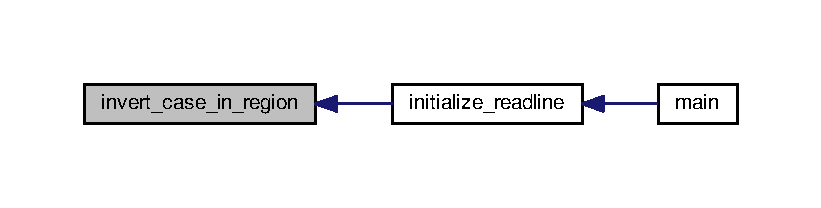
\includegraphics[width=350pt]{cle_8c_a327aaeef5e5ada52f0a64d0be178bb30_icgraph}
\end{center}
\end{figure}


\hypertarget{cle_8c_a31a3775714cbd1b923fa3ec2c5c7fd48}{\index{cle.\-c@{cle.\-c}!remove\-\_\-lines\-\_\-from\-\_\-file@{remove\-\_\-lines\-\_\-from\-\_\-file}}
\index{remove\-\_\-lines\-\_\-from\-\_\-file@{remove\-\_\-lines\-\_\-from\-\_\-file}!cle.c@{cle.\-c}}
\subsubsection[{remove\-\_\-lines\-\_\-from\-\_\-file}]{\setlength{\rightskip}{0pt plus 5cm}int remove\-\_\-lines\-\_\-from\-\_\-file (
\begin{DoxyParamCaption}
\item[{char $\ast$}]{file\-\_\-name, }
\item[{int}]{start\-\_\-line, }
\item[{int}]{line\-\_\-count}
\end{DoxyParamCaption}
)}}\label{cle_8c_a31a3775714cbd1b923fa3ec2c5c7fd48}


Removes lines from a file. 

\begin{DoxyParagraph}{Description}
This function is used to remove lines within a region of a file. It removes lines {\ttfamily  \mbox{[}start\-\_\-line.. (start\-\_\-line + line\-\_\-count) -\/ 1\mbox{]} } from the file.
\end{DoxyParagraph}

\begin{DoxyParams}{Parameters}
{\em file\-\_\-name} & The pathname of the file.\\
\hline
{\em start\-\_\-line} & The first line to remove.\\
\hline
{\em line\-\_\-count} & The number of lines to remove.\\
\hline
\end{DoxyParams}
\begin{DoxyReturn}{Returns}
Returns {\itshape -\/1} on failure, or {\itshape 0} on success. Possible reasons for failure are as follows\-: \begin{DoxyItemize}
\item The file specified by {\itshape file\-\_\-name} could not be opened. \item The specified file region is invalid.\end{DoxyItemize}

\end{DoxyReturn}
\begin{DoxySeeAlso}{See Also}
\hyperlink{cle_8h_a1e9cca6339e637e5dae988a369265b24}{count\-\_\-lines\-\_\-in\-\_\-file()}, {\itshape fopen()}, {\itshape fprintf()}, {\itshape fseek()}, {\itshape rewind()}, {\itshape malloc()}, {\itshape fgetc()}, \hyperlink{err_8h_a40bd4201ea3cf1b6f8e7fef01362bf67}{sfree()}, {\itshape fclose()}, {\itshape memmove()}, {\itshape freopen()}, \hyperlink{err_8c_a07dfb9fd24fe41a9f703bd92af2cf646}{err\-\_\-msg()}, {\itshape fwrite()}, and \hyperlink{cle_8h_ab33aa7fc65ab36bf5b799aa6521a4881}{\-\_\-readline()}. 
\end{DoxySeeAlso}


Here is the call graph for this function\-:\nopagebreak
\begin{figure}[H]
\begin{center}
\leavevmode
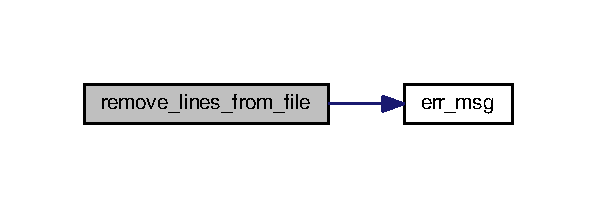
\includegraphics[width=286pt]{cle_8c_a31a3775714cbd1b923fa3ec2c5c7fd48_cgraph}
\end{center}
\end{figure}




Here is the caller graph for this function\-:\nopagebreak
\begin{figure}[H]
\begin{center}
\leavevmode
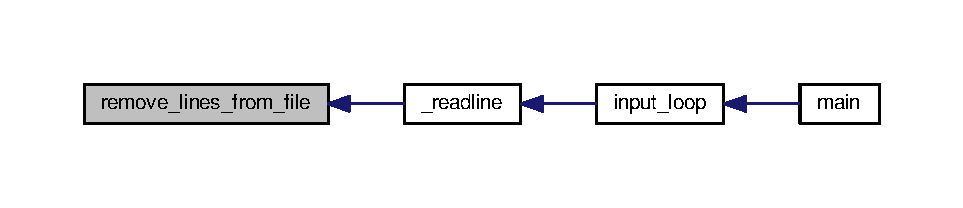
\includegraphics[width=350pt]{cle_8c_a31a3775714cbd1b923fa3ec2c5c7fd48_icgraph}
\end{center}
\end{figure}


\hypertarget{cle_8c_a8a75575085afe93be976c3d116ed8231}{\index{cle.\-c@{cle.\-c}!toggle\-\_\-editing\-\_\-mode@{toggle\-\_\-editing\-\_\-mode}}
\index{toggle\-\_\-editing\-\_\-mode@{toggle\-\_\-editing\-\_\-mode}!cle.c@{cle.\-c}}
\subsubsection[{toggle\-\_\-editing\-\_\-mode}]{\setlength{\rightskip}{0pt plus 5cm}int toggle\-\_\-editing\-\_\-mode (
\begin{DoxyParamCaption}
\item[{int}]{count, }
\item[{int}]{key}
\end{DoxyParamCaption}
)}}\label{cle_8c_a8a75575085afe93be976c3d116ed8231}


Toggles {\itshape readline} 's editing mode. 

\begin{DoxyParagraph}{Description}
This function is used to toggle {\itshape readline} 's edditing mode between {\itshape vi} mode and {\itshape emacs} mode.
\end{DoxyParagraph}
\begin{DoxyRefDesc}{Bug}
\item[\hyperlink{bug__bug000001}{Bug}]Does not work.\end{DoxyRefDesc}


\begin{DoxySeeAlso}{See Also}
{\itshape readline} . 
\end{DoxySeeAlso}


Here is the caller graph for this function\-:\nopagebreak
\begin{figure}[H]
\begin{center}
\leavevmode
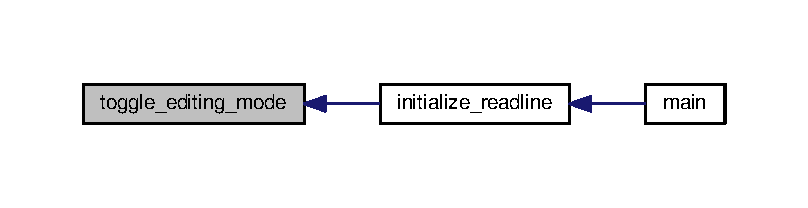
\includegraphics[width=350pt]{cle_8c_a8a75575085afe93be976c3d116ed8231_icgraph}
\end{center}
\end{figure}




\subsection{Variable Documentation}
\hypertarget{cle_8c_a2c5551422426f406568d84844b40acb9}{\index{cle.\-c@{cle.\-c}!builtins@{builtins}}
\index{builtins@{builtins}!cle.c@{cle.\-c}}
\subsubsection[{builtins}]{\setlength{\rightskip}{0pt plus 5cm}{\bf Builtin} builtins\mbox{[}$\,$\mbox{]}}}\label{cle_8c_a2c5551422426f406568d84844b40acb9}


List of shell builtins an associated function. 

\begin{DoxyParagraph}{Description}
This array stores the list of shell builtins and associated functions.
\end{DoxyParagraph}
\begin{DoxySeeAlso}{See Also}
\hyperlink{struct__builtin}{\-\_\-builtin}, \hyperlink{job_8h_a165885ac9a829b970ba29594fec5acd7}{Builtin}, \hyperlink{job_8c_a028aee0dd87474ee61f6c654efe653a2}{is\-\_\-builtin()}, \hyperlink{cle_8c_ade079408c61657dc7bbd2142a78e0e8a}{command\-\_\-completion\-\_\-generator()}, and and \hyperlink{job_8c_a328634c49391a29ef1d4e86d6bf0ea7e}{execute\-\_\-job()}. 
\end{DoxySeeAlso}
\hypertarget{cle_8c_a4a65daaf4e44aa02a8fac3ed42ec9f68}{\index{cle.\-c@{cle.\-c}!H\-I\-S\-T\-O\-R\-Y\-\_\-\-F\-I\-L\-E@{H\-I\-S\-T\-O\-R\-Y\-\_\-\-F\-I\-L\-E}}
\index{H\-I\-S\-T\-O\-R\-Y\-\_\-\-F\-I\-L\-E@{H\-I\-S\-T\-O\-R\-Y\-\_\-\-F\-I\-L\-E}!cle.c@{cle.\-c}}
\subsubsection[{H\-I\-S\-T\-O\-R\-Y\-\_\-\-F\-I\-L\-E}]{\setlength{\rightskip}{0pt plus 5cm}char H\-I\-S\-T\-O\-R\-Y\-\_\-\-F\-I\-L\-E\mbox{[}P\-A\-T\-H\-\_\-\-M\-A\-X\mbox{]}}}\label{cle_8c_a4a65daaf4e44aa02a8fac3ed42ec9f68}


Stores the path of the command history file. 

This array stores the path fo the command history file.

\begin{DoxySeeAlso}{See Also}
{\itshape readline}, {\itshape history}, \hyperlink{cle_8c_acbd58e7ffbca9f6d8d7494a053414e49}{initialize\-\_\-history()}, \hyperlink{cle_8c_a26c966f13355ca7e2a3fb8a6c3fb51c0}{N\-U\-M\-\_\-\-E\-N\-T\-R\-I\-E\-S\-\_\-\-H\-I\-S\-T\-O\-R\-Y\-\_\-\-F\-I\-L\-E}, and \hyperlink{cle_8c_a11b4616ee9e2b6f719a050b70a70b59d}{M\-A\-X\-\_\-\-N\-U\-M\-\_\-\-E\-N\-T\-R\-I\-E\-S\-\_\-\-H\-I\-S\-T\-O\-R\-Y\-\_\-\-F\-I\-L\-E}. 
\end{DoxySeeAlso}
\hypertarget{cle_8c_a2b3f51fec8189b0ed52c3a29b4d7614e}{\index{cle.\-c@{cle.\-c}!I\-N\-P\-U\-T\-R\-C\-\_\-\-F\-I\-L\-E@{I\-N\-P\-U\-T\-R\-C\-\_\-\-F\-I\-L\-E}}
\index{I\-N\-P\-U\-T\-R\-C\-\_\-\-F\-I\-L\-E@{I\-N\-P\-U\-T\-R\-C\-\_\-\-F\-I\-L\-E}!cle.c@{cle.\-c}}
\subsubsection[{I\-N\-P\-U\-T\-R\-C\-\_\-\-F\-I\-L\-E}]{\setlength{\rightskip}{0pt plus 5cm}char I\-N\-P\-U\-T\-R\-C\-\_\-\-F\-I\-L\-E\mbox{[}P\-A\-T\-H\-\_\-\-M\-A\-X\mbox{]}}}\label{cle_8c_a2b3f51fec8189b0ed52c3a29b4d7614e}


Stores the path of the {\itshape readline} input file. 

\begin{DoxyParagraph}{Description}
This array stores the path of the {\itshape readline} input file. The input file stores settings that can be used to configure the behavior of {\itshape readline}.
\end{DoxyParagraph}
\begin{DoxySeeAlso}{See Also}
\hyperlink{cle_8c_a371915dea0605bdd469053706d93951d}{initialize\-\_\-readline()}, and {\itshape readline}. 
\end{DoxySeeAlso}
\hypertarget{cle_8c_a48b5776fb79c56d2584cfa6f109e8f22}{\index{cle.\-c@{cle.\-c}!line\-\_\-buffer@{line\-\_\-buffer}}
\index{line\-\_\-buffer@{line\-\_\-buffer}!cle.c@{cle.\-c}}
\subsubsection[{line\-\_\-buffer}]{\setlength{\rightskip}{0pt plus 5cm}char$\ast$ line\-\_\-buffer = N\-U\-L\-L}}\label{cle_8c_a48b5776fb79c56d2584cfa6f109e8f22}


Stores the address of the last {\itshape readline} buffer. 

\begin{DoxyParagraph}{Description}
This pointer stores the address of the last {\itshape readline} buffer. It is aliased by \hyperlink{main_8c_ae8d7cb95bc48828d10bf3c7a31680ce2}{pipeline\-\_\-list} in \hyperlink{main_8c_af783a9705a73559f4b17ec991bc11f1e}{input\-\_\-loop()}. To avoid a possible double free expection, \hyperlink{main_8c_ae8d7cb95bc48828d10bf3c7a31680ce2}{pipeline\-\_\-list} should never be used to free the {\itshape readline} buffer.
\end{DoxyParagraph}
\begin{DoxySeeAlso}{See Also}
\hyperlink{cle_8c_a19bb8493640e845196c4d763f4109b67}{\-\_\-readline()}, {\itshape readline} , and \hyperlink{main_8c_af783a9705a73559f4b17ec991bc11f1e}{input\-\_\-loop()}. 
\end{DoxySeeAlso}
\hypertarget{cle_8c_a11b4616ee9e2b6f719a050b70a70b59d}{\index{cle.\-c@{cle.\-c}!M\-A\-X\-\_\-\-N\-U\-M\-\_\-\-E\-N\-T\-R\-I\-E\-S\-\_\-\-H\-I\-S\-T\-O\-R\-Y\-\_\-\-F\-I\-L\-E@{M\-A\-X\-\_\-\-N\-U\-M\-\_\-\-E\-N\-T\-R\-I\-E\-S\-\_\-\-H\-I\-S\-T\-O\-R\-Y\-\_\-\-F\-I\-L\-E}}
\index{M\-A\-X\-\_\-\-N\-U\-M\-\_\-\-E\-N\-T\-R\-I\-E\-S\-\_\-\-H\-I\-S\-T\-O\-R\-Y\-\_\-\-F\-I\-L\-E@{M\-A\-X\-\_\-\-N\-U\-M\-\_\-\-E\-N\-T\-R\-I\-E\-S\-\_\-\-H\-I\-S\-T\-O\-R\-Y\-\_\-\-F\-I\-L\-E}!cle.c@{cle.\-c}}
\subsubsection[{M\-A\-X\-\_\-\-N\-U\-M\-\_\-\-E\-N\-T\-R\-I\-E\-S\-\_\-\-H\-I\-S\-T\-O\-R\-Y\-\_\-\-F\-I\-L\-E}]{\setlength{\rightskip}{0pt plus 5cm}int M\-A\-X\-\_\-\-N\-U\-M\-\_\-\-E\-N\-T\-R\-I\-E\-S\-\_\-\-H\-I\-S\-T\-O\-R\-Y\-\_\-\-F\-I\-L\-E = 500}}\label{cle_8c_a11b4616ee9e2b6f719a050b70a70b59d}


Stores the maximum number of entries allowed in the command history file. 

\begin{DoxyParagraph}{Description}
This variable stores the maximum number of entries allowed in the command history file.
\end{DoxyParagraph}
\begin{DoxySeeAlso}{See Also}
{\itshape readline}, {\itshape history}, \hyperlink{cle_8c_a4a65daaf4e44aa02a8fac3ed42ec9f68}{H\-I\-S\-T\-O\-R\-Y\-\_\-\-F\-I\-L\-E}, \hyperlink{cle_8c_a26c966f13355ca7e2a3fb8a6c3fb51c0}{N\-U\-M\-\_\-\-E\-N\-T\-R\-I\-E\-S\-\_\-\-H\-I\-S\-T\-O\-R\-Y\-\_\-\-F\-I\-L\-E}, \hyperlink{cle_8c_acbd58e7ffbca9f6d8d7494a053414e49}{initialize\-\_\-history()}, and \hyperlink{cle_8c_a19bb8493640e845196c4d763f4109b67}{\-\_\-readline()}. 
\end{DoxySeeAlso}
\hypertarget{cle_8c_a26c966f13355ca7e2a3fb8a6c3fb51c0}{\index{cle.\-c@{cle.\-c}!N\-U\-M\-\_\-\-E\-N\-T\-R\-I\-E\-S\-\_\-\-H\-I\-S\-T\-O\-R\-Y\-\_\-\-F\-I\-L\-E@{N\-U\-M\-\_\-\-E\-N\-T\-R\-I\-E\-S\-\_\-\-H\-I\-S\-T\-O\-R\-Y\-\_\-\-F\-I\-L\-E}}
\index{N\-U\-M\-\_\-\-E\-N\-T\-R\-I\-E\-S\-\_\-\-H\-I\-S\-T\-O\-R\-Y\-\_\-\-F\-I\-L\-E@{N\-U\-M\-\_\-\-E\-N\-T\-R\-I\-E\-S\-\_\-\-H\-I\-S\-T\-O\-R\-Y\-\_\-\-F\-I\-L\-E}!cle.c@{cle.\-c}}
\subsubsection[{N\-U\-M\-\_\-\-E\-N\-T\-R\-I\-E\-S\-\_\-\-H\-I\-S\-T\-O\-R\-Y\-\_\-\-F\-I\-L\-E}]{\setlength{\rightskip}{0pt plus 5cm}int N\-U\-M\-\_\-\-E\-N\-T\-R\-I\-E\-S\-\_\-\-H\-I\-S\-T\-O\-R\-Y\-\_\-\-F\-I\-L\-E}}\label{cle_8c_a26c966f13355ca7e2a3fb8a6c3fb51c0}


Stores the current number of entries in the command history file. 

\begin{DoxyParagraph}{Description}
This variable stores the current number of entires in the command history file.
\end{DoxyParagraph}
\begin{DoxySeeAlso}{See Also}
{\itshape history}, {\itshape readline}, \hyperlink{cle_8c_a11b4616ee9e2b6f719a050b70a70b59d}{M\-A\-X\-\_\-\-N\-U\-M\-\_\-\-E\-N\-T\-R\-I\-E\-S\-\_\-\-H\-I\-S\-T\-O\-R\-Y\-\_\-\-F\-I\-L\-E}, \hyperlink{cle_8c_a4a65daaf4e44aa02a8fac3ed42ec9f68}{H\-I\-S\-T\-O\-R\-Y\-\_\-\-F\-I\-L\-E}, and \hyperlink{cle_8c_acbd58e7ffbca9f6d8d7494a053414e49}{initialize\-\_\-history()}. 
\end{DoxySeeAlso}

\hypertarget{cle_8h}{\section{src/cle.h File Reference}
\label{cle_8h}\index{src/cle.\-h@{src/cle.\-h}}
}


Contains function prototypes for the command line editing sub system.  


This graph shows which files directly or indirectly include this file\-:\nopagebreak
\begin{figure}[H]
\begin{center}
\leavevmode
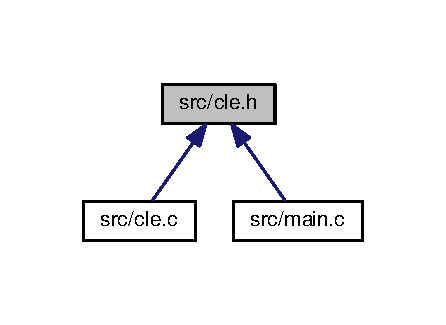
\includegraphics[width=214pt]{cle_8h__dep__incl}
\end{center}
\end{figure}
\subsection*{Functions}
\begin{DoxyCompactItemize}
\item 
int \hyperlink{cle_8h_a31a3775714cbd1b923fa3ec2c5c7fd48}{remove\-\_\-lines\-\_\-from\-\_\-file} (char $\ast$file\-\_\-name, int start\-\_\-line, int line\-\_\-count)
\begin{DoxyCompactList}\small\item\em Removes lines from a file. \end{DoxyCompactList}\item 
int \hyperlink{cle_8h_a327aaeef5e5ada52f0a64d0be178bb30}{invert\-\_\-case\-\_\-in\-\_\-region} (int count, int key)
\begin{DoxyCompactList}\small\item\em Inverts the case of characters in a region of the current line buffer of {\itshape readline} . \end{DoxyCompactList}\item 
int \hyperlink{cle_8h_a371915dea0605bdd469053706d93951d}{initialize\-\_\-readline} ()
\begin{DoxyCompactList}\small\item\em Initializes the shell's commmandline editing facilities. \end{DoxyCompactList}\item 
char $\ast$ \hyperlink{cle_8h_ab33aa7fc65ab36bf5b799aa6521a4881}{\-\_\-readline} (const char $\ast$)
\begin{DoxyCompactList}\small\item\em Calls {\itshape readline()} to read input and manages the shell's command history. \end{DoxyCompactList}\item 
int \hyperlink{cle_8h_a8a75575085afe93be976c3d116ed8231}{toggle\-\_\-editing\-\_\-mode} (int count, int key)
\begin{DoxyCompactList}\small\item\em Toggles {\itshape readline} 's editing mode. \end{DoxyCompactList}\item 
char $\ast$$\ast$ \hyperlink{cle_8h_a839745638ece1570d3c7792dfa182ae7}{command\-\_\-completion} (const char $\ast$, int, int)
\begin{DoxyCompactList}\small\item\em Registred function to perform command completion. \end{DoxyCompactList}\item 
char $\ast$ \hyperlink{cle_8h_af9de2a3a174e2493e7f3e168949bf84f}{command\-\_\-completion\-\_\-generator} (const char $\ast$, int)
\begin{DoxyCompactList}\small\item\em Generation function used for command completion. \end{DoxyCompactList}\item 
int \hyperlink{cle_8h_acbd58e7ffbca9f6d8d7494a053414e49}{initialize\-\_\-history} ()
\begin{DoxyCompactList}\small\item\em Initializes the shell's command history facilities. \end{DoxyCompactList}\item 
int \hyperlink{cle_8h_a1e9cca6339e637e5dae988a369265b24}{count\-\_\-lines\-\_\-in\-\_\-file} (const char $\ast$)
\begin{DoxyCompactList}\small\item\em Counts the number of lines in a file. \end{DoxyCompactList}\end{DoxyCompactItemize}


\subsection{Detailed Description}
Contains function prototypes for the command line editing sub system. \begin{DoxyAuthor}{Author}
Joe Nathan Abellard \{\href{https://github.com/joenatech7}{\tt https\-://github.\-com/joenatech7}\}
\end{DoxyAuthor}
\begin{DoxyDate}{Date}
September 1, 2017 
\end{DoxyDate}
\begin{DoxyParagraph}{Description}
This file contains contains function prototypes for the command lin editing sub subsystem.
\end{DoxyParagraph}
\begin{DoxySeeAlso}{See Also}
\hyperlink{cle_8c}{cle.\-c} 
\end{DoxySeeAlso}


\subsection{Function Documentation}
\hypertarget{cle_8h_ab33aa7fc65ab36bf5b799aa6521a4881}{\index{cle.\-h@{cle.\-h}!\-\_\-readline@{\-\_\-readline}}
\index{\-\_\-readline@{\-\_\-readline}!cle.h@{cle.\-h}}
\subsubsection[{\-\_\-readline}]{\setlength{\rightskip}{0pt plus 5cm}char$\ast$ \-\_\-readline (
\begin{DoxyParamCaption}
\item[{const char $\ast$}]{}
\end{DoxyParamCaption}
)}}\label{cle_8h_ab33aa7fc65ab36bf5b799aa6521a4881}


Calls {\itshape readline()} to read input and manages the shell's command history. 

\begin{DoxyParagraph}{Description}
This function is used to call @ readline() to read input from the shell prompt, and to manage the shell's command history. It does the following\-: \begin{DoxyItemize}
\item Calls \hyperlink{err_8h_a40bd4201ea3cf1b6f8e7fef01362bf67}{sfree} to de-\/allocate the memory block of the last line buffer returned by (), if nessasary. This buffer is pointed to by \hyperlink{cle_8c_a48b5776fb79c56d2584cfa6f109e8f22}{line\-\_\-buffer}. \hyperlink{cle_8c_a48b5776fb79c56d2584cfa6f109e8f22}{line\-\_\-buffer} is aliased by \hyperlink{main_8c_ae8d7cb95bc48828d10bf3c7a31680ce2}{pipeline\-\_\-list} in \hyperlink{main_8c_af783a9705a73559f4b17ec991bc11f1e}{input\-\_\-loop()}. To avoid a possible double free exeption, \hyperlink{main_8c_ae8d7cb95bc48828d10bf3c7a31680ce2}{pipeline\-\_\-list} should never be used to free the {\itshape readline} buffer. \item Calls {\itshape readline()} to read input, and assigns the location of the {\itshape readline} buffer to \hyperlink{cle_8c_a48b5776fb79c56d2584cfa6f109e8f22}{line\-\_\-buffer}. \item If the {\itshape readline} buffer is not empty, then add the line read to the history list and to the history file (\hyperlink{cle_8c_a4a65daaf4e44aa02a8fac3ed42ec9f68}{H\-I\-S\-T\-O\-R\-Y\-\_\-\-F\-I\-L\-E}). If insertion of the new entry would result in the history file having more than \hyperlink{cle_8c_a11b4616ee9e2b6f719a050b70a70b59d}{M\-A\-X\-\_\-\-N\-U\-M\-\_\-\-E\-N\-T\-R\-I\-E\-S\-\_\-\-H\-I\-S\-T\-O\-R\-Y\-\_\-\-F\-I\-L\-E}, or that the history file already contains more than M\-A\-X\-\_\-\-N\-U\-M\-\_\-\-E\-N\-T\-R\-I\-E\-S\-\_\-\-H\-I\-S\-T\-O\-R\-Y\-\_\-\-F\-I\-L\-E, then the function invokes removed\-\_\-lines\-\_\-from\-\_\-file() to remove lines from the history file before performing the insertion.\end{DoxyItemize}

\end{DoxyParagraph}

\begin{DoxyParams}{Parameters}
{\em promt\-\_\-string} & The prompt string that is displayed on the terminal.\\
\hline
\end{DoxyParams}
\begin{DoxyReturn}{Returns}
Returns \hyperlink{cle_8c_a48b5776fb79c56d2584cfa6f109e8f22}{line\-\_\-buffer}.
\end{DoxyReturn}
\begin{DoxySeeAlso}{See Also}
\hyperlink{err_8h_a40bd4201ea3cf1b6f8e7fef01362bf67}{sfree}, \hyperlink{cle_8c_a48b5776fb79c56d2584cfa6f109e8f22}{line\-\_\-buffer}, readline(), \hyperlink{cle_8c_a11b4616ee9e2b6f719a050b70a70b59d}{M\-A\-X\-\_\-\-N\-U\-M\-\_\-\-E\-N\-T\-R\-I\-E\-S\-\_\-\-H\-I\-S\-T\-O\-R\-Y\-\_\-\-F\-I\-L\-E}, \hyperlink{cle_8c_a26c966f13355ca7e2a3fb8a6c3fb51c0}{N\-U\-M\-\_\-\-E\-N\-T\-R\-I\-E\-S\-\_\-\-H\-I\-S\-T\-O\-R\-Y\-\_\-\-F\-I\-L\-E}, \hyperlink{cle_8h_a31a3775714cbd1b923fa3ec2c5c7fd48}{remove\-\_\-lines\-\_\-from\-\_\-file()}, \hyperlink{main_8c_ae8d7cb95bc48828d10bf3c7a31680ce2}{pipeline\-\_\-list}, and \hyperlink{main_8c_af783a9705a73559f4b17ec991bc11f1e}{input\-\_\-loop()}. 
\end{DoxySeeAlso}


Here is the call graph for this function\-:\nopagebreak
\begin{figure}[H]
\begin{center}
\leavevmode
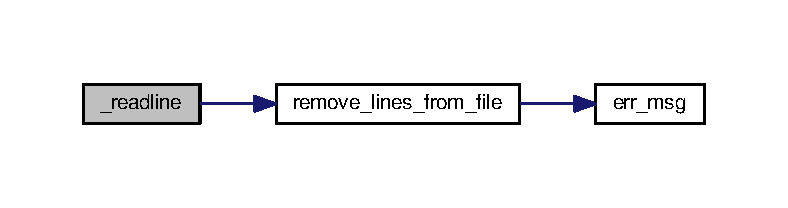
\includegraphics[width=350pt]{cle_8h_ab33aa7fc65ab36bf5b799aa6521a4881_cgraph}
\end{center}
\end{figure}




Here is the caller graph for this function\-:\nopagebreak
\begin{figure}[H]
\begin{center}
\leavevmode
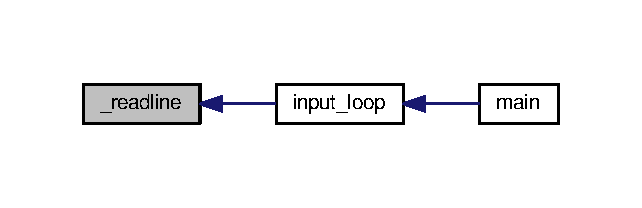
\includegraphics[width=308pt]{cle_8h_ab33aa7fc65ab36bf5b799aa6521a4881_icgraph}
\end{center}
\end{figure}


\hypertarget{cle_8h_a839745638ece1570d3c7792dfa182ae7}{\index{cle.\-h@{cle.\-h}!command\-\_\-completion@{command\-\_\-completion}}
\index{command\-\_\-completion@{command\-\_\-completion}!cle.h@{cle.\-h}}
\subsubsection[{command\-\_\-completion}]{\setlength{\rightskip}{0pt plus 5cm}char$\ast$$\ast$ command\-\_\-completion (
\begin{DoxyParamCaption}
\item[{const char $\ast$}]{, }
\item[{int}]{, }
\item[{int}]{}
\end{DoxyParamCaption}
)}}\label{cle_8h_a839745638ece1570d3c7792dfa182ae7}


Registred function to perform command completion. 

\begin{DoxyParagraph}{Description}
This function is assigned to {\itshape readline's} {\itshape rl\-\_\-attempted\-\_\-completion} variable. Consequently, when the tab key is pressed on the command line, it is invoked to perform command completion on a partial text. It uses {\itshape readline's} {\itshape rl\-\_\-completion\-\_\-matches} function with the \hyperlink{cle_8h_af9de2a3a174e2493e7f3e168949bf84f}{command\-\_\-completion\-\_\-generator()} genarator function to find possible completions for the partial text in the list of commands in the \hyperlink{job_8c_a2c5551422426f406568d84844b40acb9}{builtins} array
\end{DoxyParagraph}

\begin{DoxyParams}{Parameters}
{\em partial\-\_\-text} & The partial text to be completed.\\
\hline
{\em start} & The starting position of {\itshape partial\-\_\-text} in {\itshape readline's} line buffer.\\
\hline
{\em end} & The ending position of {\itshape partial\-\_\-text} in {\itshape readline's} line buffer.\\
\hline
\end{DoxyParams}
\begin{DoxyReturn}{Returns}
Returns an array of pointers to strings. Three outcomes are possible \-: \begin{DoxyItemize}
\item No possible completions found. In that case, the first element of the array points to N\-U\-L\-L. \item One possible completion was found. In that case, the first element of the array points to the possible completion string, and the second element points to N\-U\-L\-L. \item {\itshape n$>$=2} possible completion were found. In that case, the first {\itshape n} elements of the array point to the {\itshape n} possible completion strings, and the {\itshape }(n + 1)th element of the array points to N\-U\-L\-L.\end{DoxyItemize}

\end{DoxyReturn}
\begin{DoxySeeAlso}{See Also}
{\itshape readline} , \hyperlink{cle_8h_a371915dea0605bdd469053706d93951d}{initialize\-\_\-readline()}, command\-\_\-completion\-\_\-genarator(), and \hyperlink{job_8c_a2c5551422426f406568d84844b40acb9}{builtins}. 
\end{DoxySeeAlso}


Here is the call graph for this function\-:\nopagebreak
\begin{figure}[H]
\begin{center}
\leavevmode
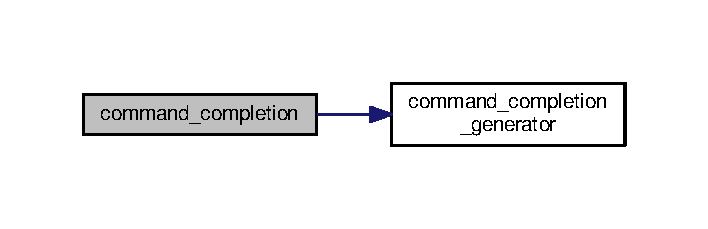
\includegraphics[width=340pt]{cle_8h_a839745638ece1570d3c7792dfa182ae7_cgraph}
\end{center}
\end{figure}




Here is the caller graph for this function\-:\nopagebreak
\begin{figure}[H]
\begin{center}
\leavevmode
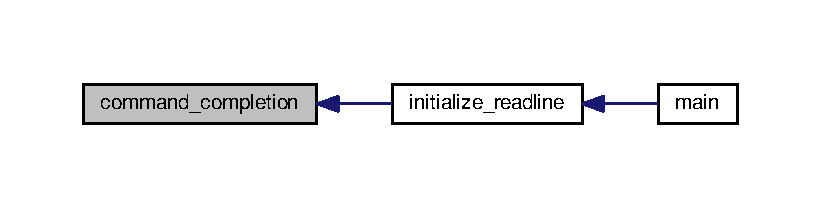
\includegraphics[width=350pt]{cle_8h_a839745638ece1570d3c7792dfa182ae7_icgraph}
\end{center}
\end{figure}


\hypertarget{cle_8h_af9de2a3a174e2493e7f3e168949bf84f}{\index{cle.\-h@{cle.\-h}!command\-\_\-completion\-\_\-generator@{command\-\_\-completion\-\_\-generator}}
\index{command\-\_\-completion\-\_\-generator@{command\-\_\-completion\-\_\-generator}!cle.h@{cle.\-h}}
\subsubsection[{command\-\_\-completion\-\_\-generator}]{\setlength{\rightskip}{0pt plus 5cm}char$\ast$ command\-\_\-completion\-\_\-generator (
\begin{DoxyParamCaption}
\item[{const char $\ast$}]{, }
\item[{int}]{}
\end{DoxyParamCaption}
)}}\label{cle_8h_af9de2a3a174e2493e7f3e168949bf84f}


Generation function used for command completion. 

\begin{DoxyParagraph}{Description}
This generation function is used by \hyperlink{cle_8h_a839745638ece1570d3c7792dfa182ae7}{command\-\_\-completion()} to find possible command completions in the \hyperlink{job_8c_a2c5551422426f406568d84844b40acb9}{builtins} array.
\end{DoxyParagraph}

\begin{DoxyParams}{Parameters}
{\em partial\-\_\-text} & The partial text to be completed.\\
\hline
{\em state} & The first time the function is called, state is {\itshape 0}. When state is zero, the function initialize some static variables.\\
\hline
\end{DoxyParams}
\begin{DoxyReturn}{Returns}
If a possible completion for {\itshape partial\-\_\-text} is found in the \hyperlink{job_8c_a2c5551422426f406568d84844b40acb9}{builtins} array, the function returns a copy to the completion string. Otherwise, it returns N\-U\-L\-L.
\end{DoxyReturn}
\begin{DoxySeeAlso}{See Also}
\hyperlink{cle_8h_a839745638ece1570d3c7792dfa182ae7}{command\-\_\-completion()}, \hyperlink{job_8c_a2c5551422426f406568d84844b40acb9}{builtins}, and {\itshape readline} . 
\end{DoxySeeAlso}


Here is the caller graph for this function\-:\nopagebreak
\begin{figure}[H]
\begin{center}
\leavevmode
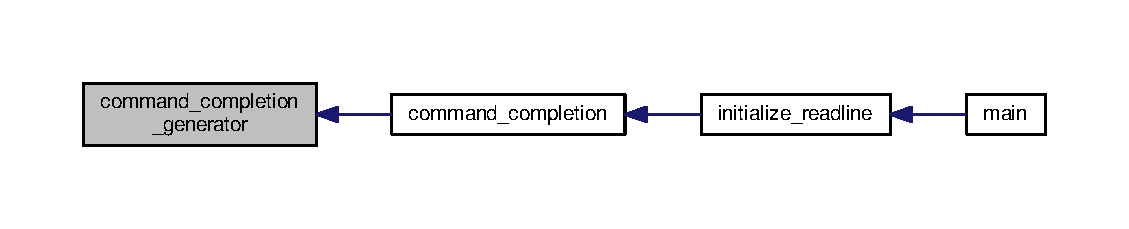
\includegraphics[width=350pt]{cle_8h_af9de2a3a174e2493e7f3e168949bf84f_icgraph}
\end{center}
\end{figure}


\hypertarget{cle_8h_a1e9cca6339e637e5dae988a369265b24}{\index{cle.\-h@{cle.\-h}!count\-\_\-lines\-\_\-in\-\_\-file@{count\-\_\-lines\-\_\-in\-\_\-file}}
\index{count\-\_\-lines\-\_\-in\-\_\-file@{count\-\_\-lines\-\_\-in\-\_\-file}!cle.h@{cle.\-h}}
\subsubsection[{count\-\_\-lines\-\_\-in\-\_\-file}]{\setlength{\rightskip}{0pt plus 5cm}int count\-\_\-lines\-\_\-in\-\_\-file (
\begin{DoxyParamCaption}
\item[{const char $\ast$}]{}
\end{DoxyParamCaption}
)}}\label{cle_8h_a1e9cca6339e637e5dae988a369265b24}


Counts the number of lines in a file. 

\begin{DoxyParagraph}{Description}
This function is used to count the number of lines in a file.
\end{DoxyParagraph}

\begin{DoxyParams}{Parameters}
{\em file\-\_\-name} & The pathname of the file.\\
\hline
\end{DoxyParams}
\begin{DoxyReturn}{Returns}
Returns {\itshape -\/1} on failure, or the number of lines in the file on success. Possible reasons for failure are as follows\-: \begin{DoxyItemize}
\item The specified file could not be opened.\end{DoxyItemize}

\end{DoxyReturn}
\begin{DoxySeeAlso}{See Also}
\hyperlink{cle_8h_a31a3775714cbd1b923fa3ec2c5c7fd48}{remove\-\_\-lines\-\_\-from\-\_\-file()}, \hyperlink{cle_8h_acbd58e7ffbca9f6d8d7494a053414e49}{initialize\-\_\-history()}, \hyperlink{cle_8c_a4a65daaf4e44aa02a8fac3ed42ec9f68}{H\-I\-S\-T\-O\-R\-Y\-\_\-\-F\-I\-L\-E}, {\itshape fopen()}, {\itshape getc()}, {\itshape fclose()}, and \hyperlink{cle_8c_a26c966f13355ca7e2a3fb8a6c3fb51c0}{N\-U\-M\-\_\-\-E\-N\-T\-R\-I\-E\-S\-\_\-\-H\-I\-S\-T\-O\-R\-Y\-\_\-\-F\-I\-L\-E}. 
\end{DoxySeeAlso}


Here is the caller graph for this function\-:\nopagebreak
\begin{figure}[H]
\begin{center}
\leavevmode
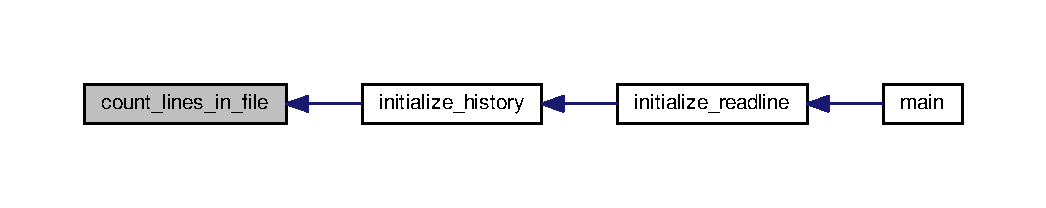
\includegraphics[width=350pt]{cle_8h_a1e9cca6339e637e5dae988a369265b24_icgraph}
\end{center}
\end{figure}


\hypertarget{cle_8h_acbd58e7ffbca9f6d8d7494a053414e49}{\index{cle.\-h@{cle.\-h}!initialize\-\_\-history@{initialize\-\_\-history}}
\index{initialize\-\_\-history@{initialize\-\_\-history}!cle.h@{cle.\-h}}
\subsubsection[{initialize\-\_\-history}]{\setlength{\rightskip}{0pt plus 5cm}int initialize\-\_\-history (
\begin{DoxyParamCaption}
{}
\end{DoxyParamCaption}
)}}\label{cle_8h_acbd58e7ffbca9f6d8d7494a053414e49}


Initializes the shell's command history facilities. 

\begin{DoxyParagraph}{Description}
This function is used to initialize the shell's command history facilities. It does the following \-: \begin{DoxyItemize}
\item Calls using\-\_\-history() to make history facilities available. \item Sets the maximum number of enties in the shell's history list to \hyperlink{cle_8c_a11b4616ee9e2b6f719a050b70a70b59d}{M\-A\-X\-\_\-\-N\-U\-M\-\_\-\-E\-N\-T\-R\-I\-E\-S\-\_\-\-H\-I\-S\-T\-O\-R\-Y\-\_\-\-F\-I\-L\-E}. \item Obtains the pathname of the shell's history file and stores the result in \hyperlink{cle_8c_a4a65daaf4e44aa02a8fac3ed42ec9f68}{H\-I\-S\-T\-O\-R\-Y\-\_\-\-F\-I\-L\-E}. \item Obtains the number of lines in the shell's history file (\hyperlink{cle_8c_a4a65daaf4e44aa02a8fac3ed42ec9f68}{H\-I\-S\-T\-O\-R\-Y\-\_\-\-F\-I\-L\-E}) via \hyperlink{cle_8h_a1e9cca6339e637e5dae988a369265b24}{count\-\_\-lines\-\_\-in\-\_\-file()} , and assigns the value to \hyperlink{cle_8c_a26c966f13355ca7e2a3fb8a6c3fb51c0}{N\-U\-M\-\_\-\-E\-N\-T\-R\-I\-E\-S\-\_\-\-H\-I\-S\-T\-O\-R\-Y\-\_\-\-F\-I\-L\-E}. \item Reads history from the history file (\hyperlink{cle_8c_a4a65daaf4e44aa02a8fac3ed42ec9f68}{H\-I\-S\-T\-O\-R\-Y\-\_\-\-F\-I\-L\-E}) into the shell's history list. \item Disables the recording of timestamps for history entries.\end{DoxyItemize}

\end{DoxyParagraph}
\begin{DoxyReturn}{Returns}
Returns {\itshape void}.
\end{DoxyReturn}
\begin{DoxySeeAlso}{See Also}
and \hyperlink{cle_8h_a371915dea0605bdd469053706d93951d}{initialize\-\_\-readline()}. \hyperlink{cle_8c_a11b4616ee9e2b6f719a050b70a70b59d}{M\-A\-X\-\_\-\-N\-U\-M\-\_\-\-E\-N\-T\-R\-I\-E\-S\-\_\-\-H\-I\-S\-T\-O\-R\-Y\-\_\-\-F\-I\-L\-E}, \hyperlink{cle_8c_a4a65daaf4e44aa02a8fac3ed42ec9f68}{H\-I\-S\-T\-O\-R\-Y\-\_\-\-F\-I\-L\-E}, \hyperlink{cle_8c_a26c966f13355ca7e2a3fb8a6c3fb51c0}{N\-U\-M\-\_\-\-E\-N\-T\-R\-I\-E\-S\-\_\-\-H\-I\-S\-T\-O\-R\-Y\-\_\-\-F\-I\-L\-E}, \hyperlink{cle_8h_a1e9cca6339e637e5dae988a369265b24}{count\-\_\-lines\-\_\-in\-\_\-file()}, 
\end{DoxySeeAlso}


Here is the call graph for this function\-:\nopagebreak
\begin{figure}[H]
\begin{center}
\leavevmode
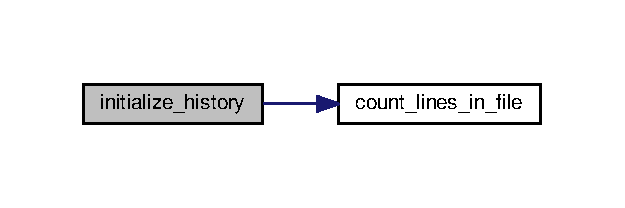
\includegraphics[width=300pt]{cle_8h_acbd58e7ffbca9f6d8d7494a053414e49_cgraph}
\end{center}
\end{figure}




Here is the caller graph for this function\-:\nopagebreak
\begin{figure}[H]
\begin{center}
\leavevmode
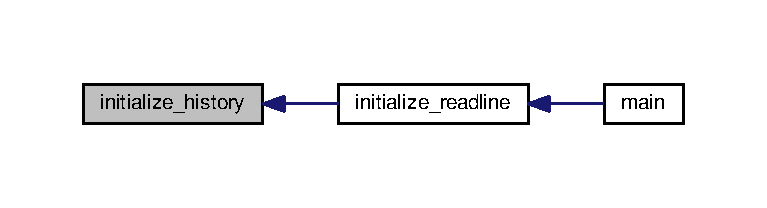
\includegraphics[width=350pt]{cle_8h_acbd58e7ffbca9f6d8d7494a053414e49_icgraph}
\end{center}
\end{figure}


\hypertarget{cle_8h_a371915dea0605bdd469053706d93951d}{\index{cle.\-h@{cle.\-h}!initialize\-\_\-readline@{initialize\-\_\-readline}}
\index{initialize\-\_\-readline@{initialize\-\_\-readline}!cle.h@{cle.\-h}}
\subsubsection[{initialize\-\_\-readline}]{\setlength{\rightskip}{0pt plus 5cm}int initialize\-\_\-readline (
\begin{DoxyParamCaption}
{}
\end{DoxyParamCaption}
)}}\label{cle_8h_a371915dea0605bdd469053706d93951d}


Initializes the shell's commmandline editing facilities. 

\begin{DoxyParagraph}{Description}
This function is used to initialize the shell's commandline editing facilities. It does the following \-: \begin{DoxyItemize}
\item Calls \hyperlink{cle_8h_acbd58e7ffbca9f6d8d7494a053414e49}{initialize\-\_\-history()} to initialize the shell's command history facilities. \item Registers the shell's command completion function (\hyperlink{cle_8h_a839745638ece1570d3c7792dfa182ae7}{command\-\_\-completion()}). \item Registers custom binable functions (\hyperlink{cle_8h_a327aaeef5e5ada52f0a64d0be178bb30}{invert\-\_\-case\-\_\-in\-\_\-region()}, and \hyperlink{cle_8h_a8a75575085afe93be976c3d116ed8231}{toggle\-\_\-editing\-\_\-mode()}). \item Obtains the path of {\itshape readline} 's {\itshape inputrc} file and assign the value to \hyperlink{cle_8c_a2b3f51fec8189b0ed52c3a29b4d7614e}{I\-N\-P\-U\-T\-R\-C\-\_\-\-F\-I\-L\-E}. \item Sets the I\-N\-P\-U\-T\-R\-C environment variable. \item Reads settings from the input file (\hyperlink{cle_8c_a2b3f51fec8189b0ed52c3a29b4d7614e}{I\-N\-P\-U\-T\-R\-C\-\_\-\-F\-I\-L\-E}).\end{DoxyItemize}

\end{DoxyParagraph}
\begin{DoxyReturn}{Returns}
Returns {\itshape -\/1} on failure, or {\itshape 0} on success.
\end{DoxyReturn}
\begin{DoxySeeAlso}{See Also}
\hyperlink{cle_8h_acbd58e7ffbca9f6d8d7494a053414e49}{initialize\-\_\-history()}, \hyperlink{cle_8h_a839745638ece1570d3c7792dfa182ae7}{command\-\_\-completion()}, \hyperlink{cle_8h_a327aaeef5e5ada52f0a64d0be178bb30}{invert\-\_\-case\-\_\-in\-\_\-region()}, \hyperlink{cle_8h_a8a75575085afe93be976c3d116ed8231}{toggle\-\_\-editing\-\_\-mode()}, \hyperlink{cle_8c_a2b3f51fec8189b0ed52c3a29b4d7614e}{I\-N\-P\-U\-T\-R\-C\-\_\-\-F\-I\-L\-E}, {\itshape readline} , {\itshape inputrc}, and (). 
\end{DoxySeeAlso}


Here is the call graph for this function\-:\nopagebreak
\begin{figure}[H]
\begin{center}
\leavevmode
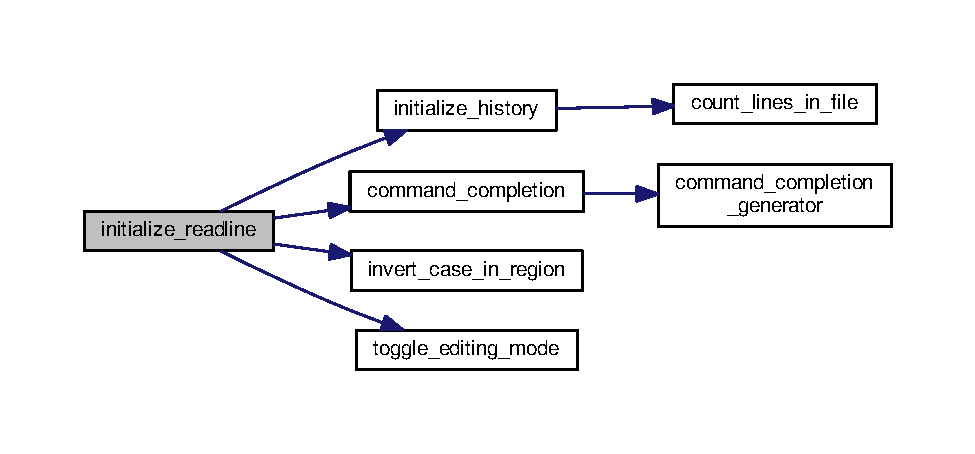
\includegraphics[width=350pt]{cle_8h_a371915dea0605bdd469053706d93951d_cgraph}
\end{center}
\end{figure}




Here is the caller graph for this function\-:\nopagebreak
\begin{figure}[H]
\begin{center}
\leavevmode
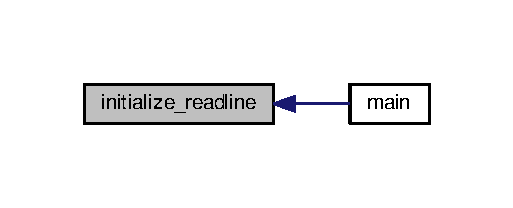
\includegraphics[width=246pt]{cle_8h_a371915dea0605bdd469053706d93951d_icgraph}
\end{center}
\end{figure}


\hypertarget{cle_8h_a327aaeef5e5ada52f0a64d0be178bb30}{\index{cle.\-h@{cle.\-h}!invert\-\_\-case\-\_\-in\-\_\-region@{invert\-\_\-case\-\_\-in\-\_\-region}}
\index{invert\-\_\-case\-\_\-in\-\_\-region@{invert\-\_\-case\-\_\-in\-\_\-region}!cle.h@{cle.\-h}}
\subsubsection[{invert\-\_\-case\-\_\-in\-\_\-region}]{\setlength{\rightskip}{0pt plus 5cm}int invert\-\_\-case\-\_\-in\-\_\-region (
\begin{DoxyParamCaption}
\item[{int}]{count, }
\item[{int}]{key}
\end{DoxyParamCaption}
)}}\label{cle_8h_a327aaeef5e5ada52f0a64d0be178bb30}


Inverts the case of characters in a region of the current line buffer of {\itshape readline} . 

\begin{DoxyParagraph}{Description}
This function is used to inverts the case of characters in a region of the current line buffer of {\itshape readline}.
\end{DoxyParagraph}

\begin{DoxyParams}{Parameters}
{\em count} & The number of characters whose case is to be inverted.\\
\hline
{\em key} & Not used in the function.\\
\hline
\end{DoxyParams}
\begin{DoxyReturn}{Returns}
Return {\itshape -\/1} on failure, or the number of characters inverted on success.
\end{DoxyReturn}
\begin{DoxySeeAlso}{See Also}
{\itshape readline}, and \hyperlink{cle_8h_a371915dea0605bdd469053706d93951d}{initialize\-\_\-readline()}. 
\end{DoxySeeAlso}


Here is the caller graph for this function\-:\nopagebreak
\begin{figure}[H]
\begin{center}
\leavevmode
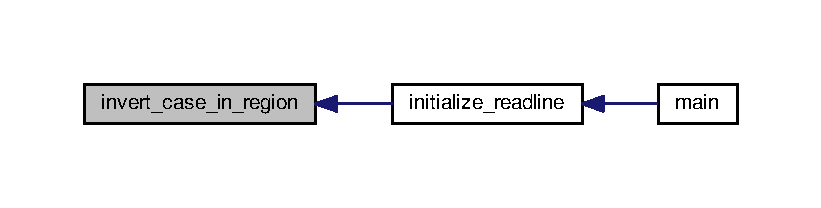
\includegraphics[width=350pt]{cle_8h_a327aaeef5e5ada52f0a64d0be178bb30_icgraph}
\end{center}
\end{figure}


\hypertarget{cle_8h_a31a3775714cbd1b923fa3ec2c5c7fd48}{\index{cle.\-h@{cle.\-h}!remove\-\_\-lines\-\_\-from\-\_\-file@{remove\-\_\-lines\-\_\-from\-\_\-file}}
\index{remove\-\_\-lines\-\_\-from\-\_\-file@{remove\-\_\-lines\-\_\-from\-\_\-file}!cle.h@{cle.\-h}}
\subsubsection[{remove\-\_\-lines\-\_\-from\-\_\-file}]{\setlength{\rightskip}{0pt plus 5cm}int remove\-\_\-lines\-\_\-from\-\_\-file (
\begin{DoxyParamCaption}
\item[{char $\ast$}]{file\-\_\-name, }
\item[{int}]{start\-\_\-line, }
\item[{int}]{line\-\_\-count}
\end{DoxyParamCaption}
)}}\label{cle_8h_a31a3775714cbd1b923fa3ec2c5c7fd48}


Removes lines from a file. 

\begin{DoxyParagraph}{Description}
This function is used to remove lines within a region of a file. It removes lines {\ttfamily  \mbox{[}start\-\_\-line.. (start\-\_\-line + line\-\_\-count) -\/ 1\mbox{]} } from the file.
\end{DoxyParagraph}

\begin{DoxyParams}{Parameters}
{\em file\-\_\-name} & The pathname of the file.\\
\hline
{\em start\-\_\-line} & The first line to remove.\\
\hline
{\em line\-\_\-count} & The number of lines to remove.\\
\hline
\end{DoxyParams}
\begin{DoxyReturn}{Returns}
Returns {\itshape -\/1} on failure, or {\itshape 0} on success. Possible reasons for failure are as follows\-: \begin{DoxyItemize}
\item The file specified by {\itshape file\-\_\-name} could not be opened. \item The specified file region is invalid.\end{DoxyItemize}

\end{DoxyReturn}
\begin{DoxySeeAlso}{See Also}
\hyperlink{cle_8h_a1e9cca6339e637e5dae988a369265b24}{count\-\_\-lines\-\_\-in\-\_\-file()}, {\itshape fopen()}, {\itshape fprintf()}, {\itshape fseek()}, {\itshape rewind()}, {\itshape malloc()}, {\itshape fgetc()}, \hyperlink{err_8h_a40bd4201ea3cf1b6f8e7fef01362bf67}{sfree()}, {\itshape fclose()}, {\itshape memmove()}, {\itshape freopen()}, \hyperlink{err_8c_a07dfb9fd24fe41a9f703bd92af2cf646}{err\-\_\-msg()}, {\itshape fwrite()}, and \hyperlink{cle_8h_ab33aa7fc65ab36bf5b799aa6521a4881}{\-\_\-readline()}. 
\end{DoxySeeAlso}


Here is the call graph for this function\-:\nopagebreak
\begin{figure}[H]
\begin{center}
\leavevmode
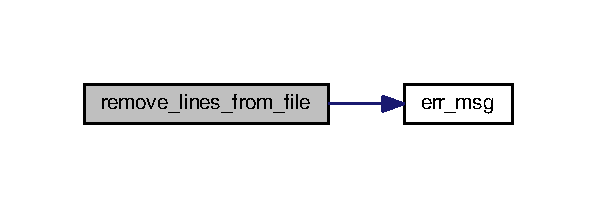
\includegraphics[width=286pt]{cle_8h_a31a3775714cbd1b923fa3ec2c5c7fd48_cgraph}
\end{center}
\end{figure}




Here is the caller graph for this function\-:\nopagebreak
\begin{figure}[H]
\begin{center}
\leavevmode
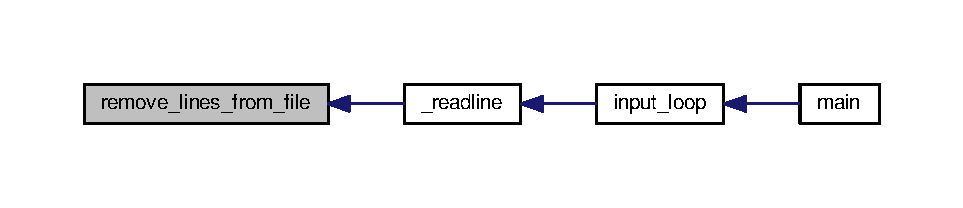
\includegraphics[width=350pt]{cle_8h_a31a3775714cbd1b923fa3ec2c5c7fd48_icgraph}
\end{center}
\end{figure}


\hypertarget{cle_8h_a8a75575085afe93be976c3d116ed8231}{\index{cle.\-h@{cle.\-h}!toggle\-\_\-editing\-\_\-mode@{toggle\-\_\-editing\-\_\-mode}}
\index{toggle\-\_\-editing\-\_\-mode@{toggle\-\_\-editing\-\_\-mode}!cle.h@{cle.\-h}}
\subsubsection[{toggle\-\_\-editing\-\_\-mode}]{\setlength{\rightskip}{0pt plus 5cm}int toggle\-\_\-editing\-\_\-mode (
\begin{DoxyParamCaption}
\item[{int}]{count, }
\item[{int}]{key}
\end{DoxyParamCaption}
)}}\label{cle_8h_a8a75575085afe93be976c3d116ed8231}


Toggles {\itshape readline} 's editing mode. 

\begin{DoxyParagraph}{Description}
This function is used to toggle {\itshape readline} 's edditing mode between {\itshape vi} mode and {\itshape emacs} mode.
\end{DoxyParagraph}
\begin{DoxyRefDesc}{Bug}
\item[\hyperlink{bug__bug000001}{Bug}]Does not work.\end{DoxyRefDesc}


\begin{DoxySeeAlso}{See Also}
{\itshape readline} . 
\end{DoxySeeAlso}


Here is the caller graph for this function\-:\nopagebreak
\begin{figure}[H]
\begin{center}
\leavevmode
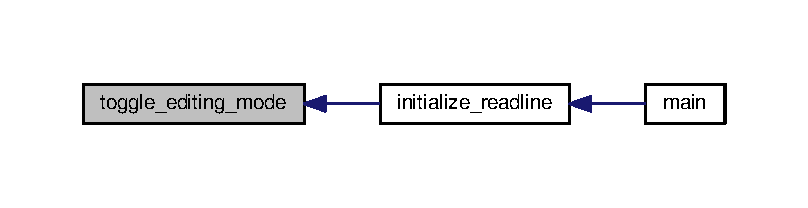
\includegraphics[width=350pt]{cle_8h_a8a75575085afe93be976c3d116ed8231_icgraph}
\end{center}
\end{figure}



\hypertarget{err_8c}{\section{src/err.c File Reference}
\label{err_8c}\index{src/err.\-c@{src/err.\-c}}
}


Contains code for the error handling subsystem.  


{\ttfamily \#include $<$stdio.\-h$>$}\\*
{\ttfamily \#include $<$stdlib.\-h$>$}\\*
{\ttfamily \#include $<$errno.\-h$>$}\\*
{\ttfamily \#include $<$unistd.\-h$>$}\\*
{\ttfamily \#include $<$string.\-h$>$}\\*
{\ttfamily \#include \char`\"{}err.\-h\char`\"{}}\\*
Include dependency graph for err.\-c\-:\nopagebreak
\begin{figure}[H]
\begin{center}
\leavevmode
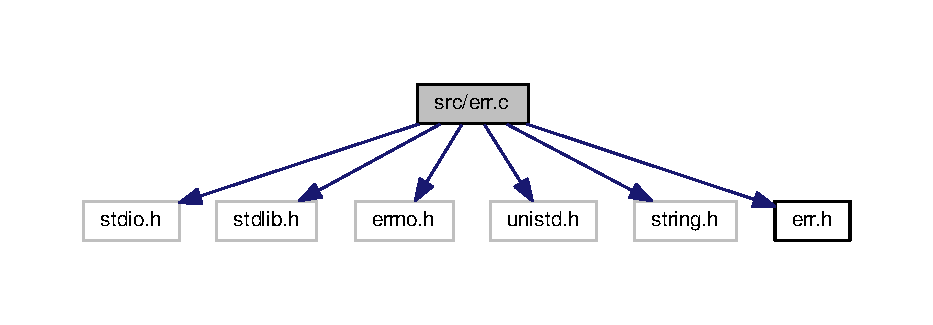
\includegraphics[width=350pt]{err_8c__incl}
\end{center}
\end{figure}
\subsection*{Macros}
\begin{DoxyCompactItemize}
\item 
\hypertarget{err_8c_a95fc89eab89c62fc880a852fa1fe969f}{\#define {\bfseries M\-A\-X\-\_\-\-E\-N\-A\-M\-E}~133}\label{err_8c_a95fc89eab89c62fc880a852fa1fe969f}

\end{DoxyCompactItemize}
\subsection*{Functions}
\begin{DoxyCompactItemize}
\item 
void \hyperlink{err_8c_a7a249a2d9b54b1c4c9a43a9d302d637e}{safe\-\_\-free} (void $\ast$$\ast$pp)
\begin{DoxyCompactList}\small\item\em Safer version of free. \end{DoxyCompactList}\item 
void \hyperlink{err_8c_a07dfb9fd24fe41a9f703bd92af2cf646}{err\-\_\-msg} (const char $\ast$user\-\_\-msg)
\begin{DoxyCompactList}\small\item\em Prints an error message corresponding to the current value of {\itshape errno}. \end{DoxyCompactList}\item 
void \hyperlink{err_8c_a8e8952208174427fc9de79dfed72b043}{terminate} (int use\-\_\-exit3)
\begin{DoxyCompactList}\small\item\em Terminates the calling process. \end{DoxyCompactList}\item 
void \hyperlink{err_8c_ab24204e73fd5cdd4d62dc30f4794da23}{err\-\_\-exit} (const char $\ast$user\-\_\-msg)
\begin{DoxyCompactList}\small\item\em Prints and error message, and terminates the calling process. \end{DoxyCompactList}\item 
void \hyperlink{err_8c_ad8feb10c9562b2de6dd93677d4d326af}{err\-\_\-\-\_\-exit} (const char $\ast$user\-\_\-msg)
\begin{DoxyCompactList}\small\item\em Prints and error message, and terminates the calling process. \end{DoxyCompactList}\end{DoxyCompactItemize}


\subsection{Detailed Description}
Contains code for the error handling subsystem. \begin{DoxyAuthor}{Author}
Joe Nathan Abellard \{\href{https://github.com/joenatech7}{\tt https\-://github.\-com/joenatech7}\}
\end{DoxyAuthor}
\begin{DoxyDate}{Date}
September 1, 2017 
\end{DoxyDate}
\begin{DoxyParagraph}{Description}
This file contains contains code for the error handling sub system.
\end{DoxyParagraph}
\begin{DoxySeeAlso}{See Also}
\hyperlink{err_8h}{err.\-h} 
\end{DoxySeeAlso}


\subsection{Function Documentation}
\hypertarget{err_8c_ad8feb10c9562b2de6dd93677d4d326af}{\index{err.\-c@{err.\-c}!err\-\_\-\-\_\-exit@{err\-\_\-\-\_\-exit}}
\index{err\-\_\-\-\_\-exit@{err\-\_\-\-\_\-exit}!err.c@{err.\-c}}
\subsubsection[{err\-\_\-\-\_\-exit}]{\setlength{\rightskip}{0pt plus 5cm}void err\-\_\-\-\_\-exit (
\begin{DoxyParamCaption}
\item[{const char $\ast$}]{user\-\_\-msg}
\end{DoxyParamCaption}
)}}\label{err_8c_ad8feb10c9562b2de6dd93677d4d326af}


Prints and error message, and terminates the calling process. 

\begin{DoxyParagraph}{Description}
This function is used to print an error message and then terminate the calling process. It prints the error message by calling \hyperlink{err_8h_a07dfb9fd24fe41a9f703bd92af2cf646}{err\-\_\-msg()}, and then terminates the process by calling \hyperlink{err_8h_a8e8952208174427fc9de79dfed72b043}{terminate()} wiht the value {\itshape 1} .
\end{DoxyParagraph}

\begin{DoxyParams}{Parameters}
{\em user\-\_\-msg} & This string is passed to \hyperlink{err_8h_a07dfb9fd24fe41a9f703bd92af2cf646}{err\-\_\-msg()}.\\
\hline
\end{DoxyParams}
\begin{DoxyReturn}{Returns}
Returns {\itshape void}.
\end{DoxyReturn}
\begin{DoxySeeAlso}{See Also}
\hyperlink{err_8h_a07dfb9fd24fe41a9f703bd92af2cf646}{err\-\_\-msg()}, \hyperlink{err_8h_a8e8952208174427fc9de79dfed72b043}{terminate()}, and \hyperlink{err_8h_abdf2524e566eb527094c786e60c4e15a}{err\-\_\-exit()}. 
\end{DoxySeeAlso}


Here is the call graph for this function\-:\nopagebreak
\begin{figure}[H]
\begin{center}
\leavevmode
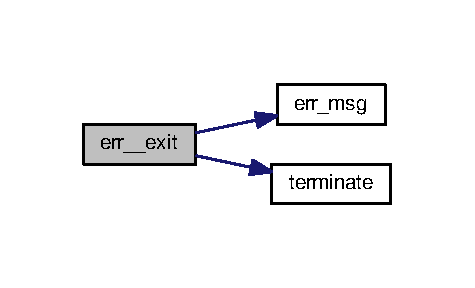
\includegraphics[width=228pt]{err_8c_ad8feb10c9562b2de6dd93677d4d326af_cgraph}
\end{center}
\end{figure}


\hypertarget{err_8c_ab24204e73fd5cdd4d62dc30f4794da23}{\index{err.\-c@{err.\-c}!err\-\_\-exit@{err\-\_\-exit}}
\index{err\-\_\-exit@{err\-\_\-exit}!err.c@{err.\-c}}
\subsubsection[{err\-\_\-exit}]{\setlength{\rightskip}{0pt plus 5cm}void err\-\_\-exit (
\begin{DoxyParamCaption}
\item[{const char $\ast$}]{user\-\_\-msg}
\end{DoxyParamCaption}
)}}\label{err_8c_ab24204e73fd5cdd4d62dc30f4794da23}


Prints and error message, and terminates the calling process. 

\begin{DoxyParagraph}{Description}
This function is used to print an error message and then terminate the calling process. It prints the error message by calling \hyperlink{err_8h_a07dfb9fd24fe41a9f703bd92af2cf646}{err\-\_\-msg()}, and then terminates the process by calling \hyperlink{err_8h_a8e8952208174427fc9de79dfed72b043}{terminate()} wiht the value {\itshape 0} .
\end{DoxyParagraph}

\begin{DoxyParams}{Parameters}
{\em user\-\_\-msg} & This string is passed to \hyperlink{err_8h_a07dfb9fd24fe41a9f703bd92af2cf646}{err\-\_\-msg()}.\\
\hline
\end{DoxyParams}
\begin{DoxyReturn}{Returns}
Returns {\itshape void}.
\end{DoxyReturn}
\begin{DoxySeeAlso}{See Also}
\hyperlink{err_8h_a07dfb9fd24fe41a9f703bd92af2cf646}{err\-\_\-msg()}, \hyperlink{err_8h_a8e8952208174427fc9de79dfed72b043}{terminate()}, and \hyperlink{err_8h_a30a51bd316b9e22534d7d2c50c110e9e}{err\-\_\-\-\_\-exit()}. 
\end{DoxySeeAlso}


Here is the call graph for this function\-:\nopagebreak
\begin{figure}[H]
\begin{center}
\leavevmode
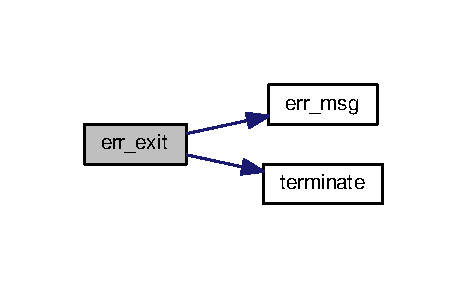
\includegraphics[width=224pt]{err_8c_ab24204e73fd5cdd4d62dc30f4794da23_cgraph}
\end{center}
\end{figure}




Here is the caller graph for this function\-:\nopagebreak
\begin{figure}[H]
\begin{center}
\leavevmode
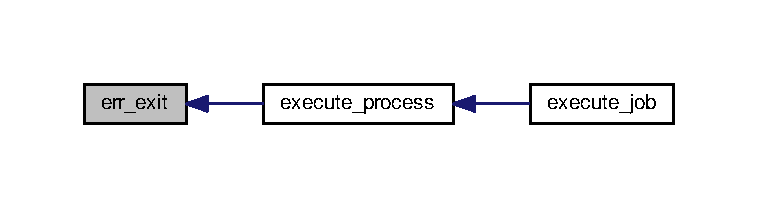
\includegraphics[width=350pt]{err_8c_ab24204e73fd5cdd4d62dc30f4794da23_icgraph}
\end{center}
\end{figure}


\hypertarget{err_8c_a07dfb9fd24fe41a9f703bd92af2cf646}{\index{err.\-c@{err.\-c}!err\-\_\-msg@{err\-\_\-msg}}
\index{err\-\_\-msg@{err\-\_\-msg}!err.c@{err.\-c}}
\subsubsection[{err\-\_\-msg}]{\setlength{\rightskip}{0pt plus 5cm}void err\-\_\-msg (
\begin{DoxyParamCaption}
\item[{const char $\ast$}]{user\-\_\-msg}
\end{DoxyParamCaption}
)}}\label{err_8c_a07dfb9fd24fe41a9f703bd92af2cf646}


Prints an error message corresponding to the current value of {\itshape errno}. 

\begin{DoxyParagraph}{Description}
This function is used to print an error message coresponding to the current value of . It is a more verbose version of the standard {\itshape perror()} function.
\end{DoxyParagraph}

\begin{DoxyParams}{Parameters}
{\em user\-\_\-msg} & This string prefixes the error message that will be printed.\\
\hline
\end{DoxyParams}
\begin{DoxyReturn}{Returns}
Returns {\itshape void}.
\end{DoxyReturn}
\begin{DoxySeeAlso}{See Also}
{\itshape perror()}, {\itshape errno}, {\itshape malloc()}, {\itshape sprintf()}, {\itshape fflush()}, \hyperlink{err_8h_a8e8952208174427fc9de79dfed72b043}{terminate()}, \hyperlink{err_8h_abdf2524e566eb527094c786e60c4e15a}{err\-\_\-exit()}, {\itshape fputs()}, \hyperlink{err_8h_a40bd4201ea3cf1b6f8e7fef01362bf67}{sfree()}, and \hyperlink{err_8h_a30a51bd316b9e22534d7d2c50c110e9e}{err\-\_\-\-\_\-exit()}. 
\end{DoxySeeAlso}


Here is the caller graph for this function\-:\nopagebreak
\begin{figure}[H]
\begin{center}
\leavevmode
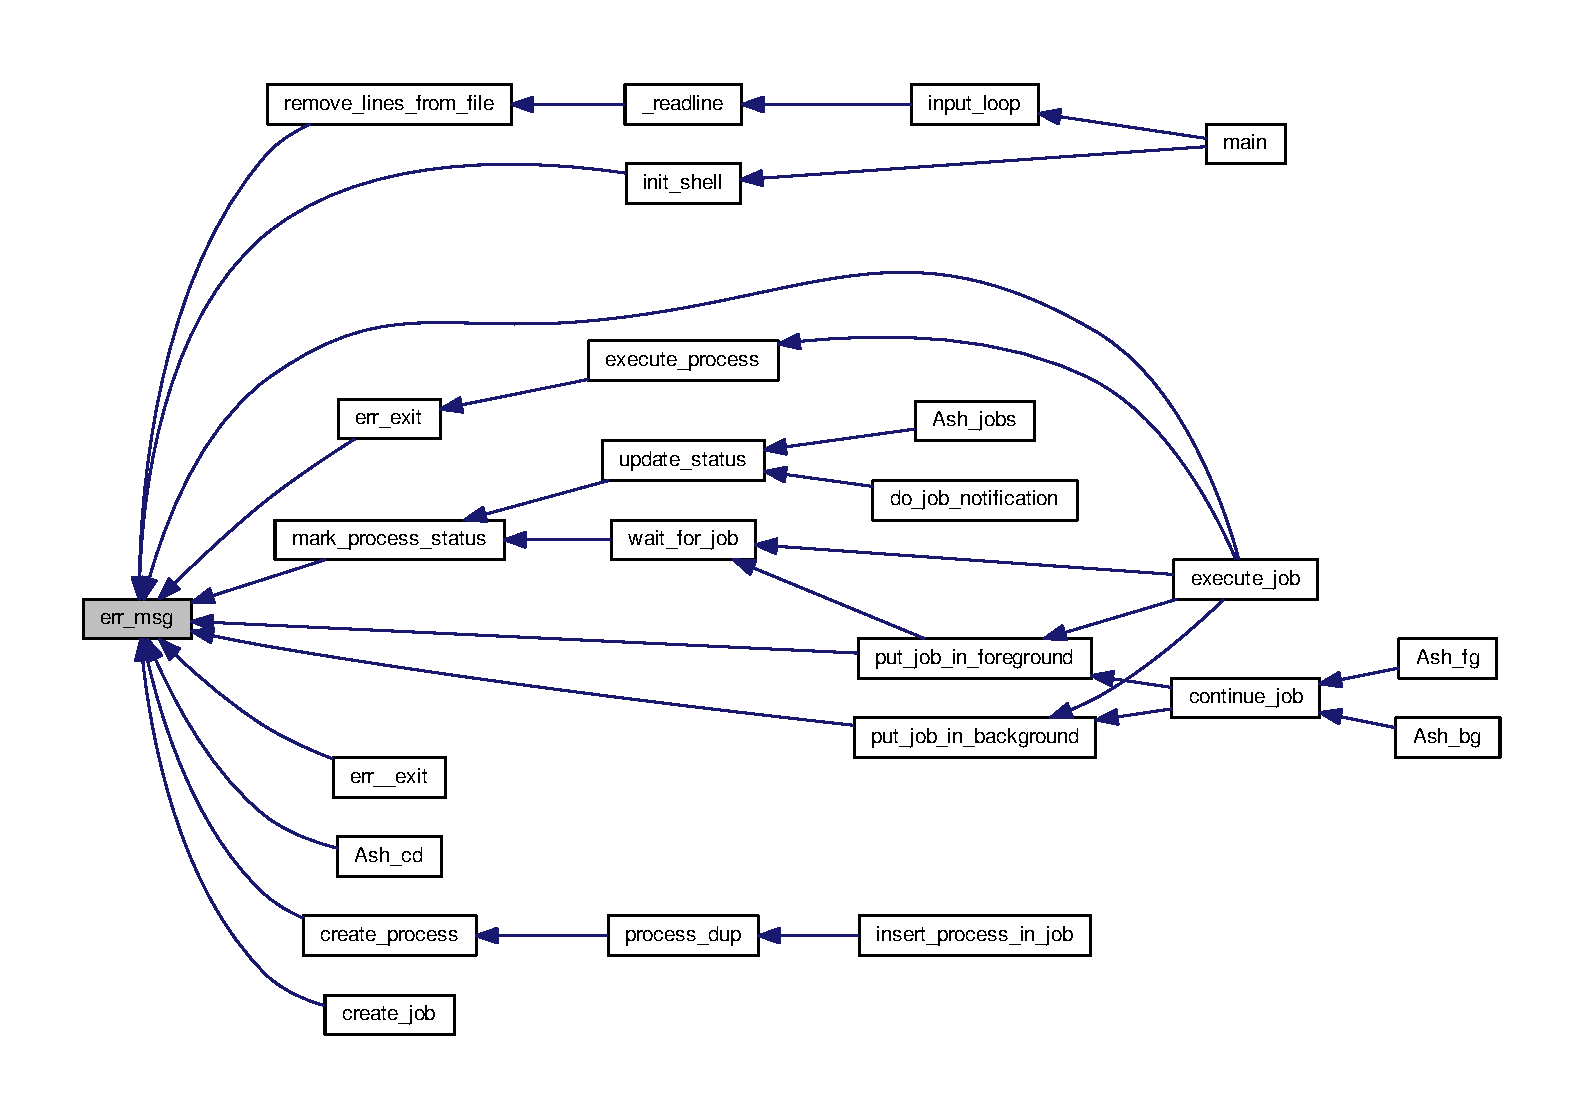
\includegraphics[width=350pt]{err_8c_a07dfb9fd24fe41a9f703bd92af2cf646_icgraph}
\end{center}
\end{figure}


\hypertarget{err_8c_a7a249a2d9b54b1c4c9a43a9d302d637e}{\index{err.\-c@{err.\-c}!safe\-\_\-free@{safe\-\_\-free}}
\index{safe\-\_\-free@{safe\-\_\-free}!err.c@{err.\-c}}
\subsubsection[{safe\-\_\-free}]{\setlength{\rightskip}{0pt plus 5cm}void safe\-\_\-free (
\begin{DoxyParamCaption}
\item[{void $\ast$$\ast$}]{pp}
\end{DoxyParamCaption}
)}}\label{err_8c_a7a249a2d9b54b1c4c9a43a9d302d637e}


Safer version of free. 

\begin{DoxyParagraph}{Description}
This function is a safer version of {\itshape free()}, which is used for de-\/allocating memory from the heap. The are two potential pillfalls when using the standard {\itshape free()} function\-: (1) passing it a N\-U\-L\-L pointer, which results in a run-\/time exeption, and (2) passing it a pointer to a memory block that has already been previously de-\/allocated, resulting in a double free exeption. It is good practice to ensure that (1) a pointer that is to be passed is {\itshape free()} is non-\/\-N\-U\-L\-L, and (2) and to assign N\-U\-L\-L to a pointer right after the memory block it points to has been de-\/allocated with {\itshape free()} . Doing (1) can be inconvinient, and since a pointer is only passed by value to {\itshape free()}, {\itshape free()} can not do (2) on behalf of the programmer. \hyperlink{err_8h_a7a249a2d9b54b1c4c9a43a9d302d637e}{safe\-\_\-free()} seeks to eliminate these inconveniences. It calls {\itshape free()} internally to de-\/allocate memory, but does some things differently than {\itshape free()}. Before calling {\itshape free()} \hyperlink{err_8h_a7a249a2d9b54b1c4c9a43a9d302d637e}{safe\-\_\-free()} checks if the pointer to the momory block is N\-U\-L\-L, and if that is the case, does nothing. Otherwise, it calls {\itshape free()} to de-\/allocate the memory block. It's argument is a pointer to pointer pointing to memory block to be de-\/allocated (i.\-e, a double pointer). Accepting a double pointer allows it to assign N\-U\-L\-L to the pointer after the memory de-\/allocation.
\end{DoxyParagraph}

\begin{DoxyParams}{Parameters}
{\em pp} & Pointer to the pointer pointing to the memory block to be de-\/allocated.\\
\hline
\end{DoxyParams}
\begin{DoxyReturn}{Returns}
returns {\itshape void} 
\end{DoxyReturn}
\begin{DoxySeeAlso}{See Also}
\hyperlink{err_8h_a40bd4201ea3cf1b6f8e7fef01362bf67}{sfree(p)}, and {\itshape free()} 
\end{DoxySeeAlso}
\hypertarget{err_8c_a8e8952208174427fc9de79dfed72b043}{\index{err.\-c@{err.\-c}!terminate@{terminate}}
\index{terminate@{terminate}!err.c@{err.\-c}}
\subsubsection[{terminate}]{\setlength{\rightskip}{0pt plus 5cm}void terminate (
\begin{DoxyParamCaption}
\item[{int}]{use\-\_\-exit3}
\end{DoxyParamCaption}
)}}\label{err_8c_a8e8952208174427fc9de79dfed72b043}


Terminates the calling process. 

\begin{DoxyParagraph}{Description}
This function is used to terminate the calling process. It does that by calling either {\itshape abort()} , {\itshape exit()} , or {\itshape \-\_\-exit()} . If the environment variable E\-F\-\_\-\-D\-U\-M\-P\-C\-O\-R\-E is defined, and is a non-\/empty string, it ends the process by calling {\itshape abort()}. Otherwise the function ends the process by calling either {\itshape exit()} , or {\itshape \-\_\-exit()} .
\end{DoxyParagraph}

\begin{DoxyParams}{Parameters}
{\em use\-\_\-exit3} & This interger determines whether the function calls {\itshape exit()} , or {\itshape \-\_\-exit()} . If it is non-\/zero, it calls {\itshape exit()} with the value E\-X\-I\-T\-\_\-\-F\-A\-I\-L\-U\-R\-E, otherwise it calls {\itshape \-\_\-exit()} with the value E\-X\-I\-T\-\_\-\-F\-A\-I\-L\-U\-R\-E.\\
\hline
\end{DoxyParams}
\begin{DoxyReturn}{Returns}
Returns {\itshape void}.
\end{DoxyReturn}
\begin{DoxySeeAlso}{See Also}
E\-F\-\_\-\-D\-U\-M\-P\-C\-O\-R\-E, {\itshape exit()}, {\itshape \-\_\-exit()}, {\itshape abort()}, \hyperlink{err_8h_a07dfb9fd24fe41a9f703bd92af2cf646}{err\-\_\-msg()}, \hyperlink{err_8h_abdf2524e566eb527094c786e60c4e15a}{err\-\_\-exit()}, E\-X\-I\-T\-\_\-\-F\-A\-I\-L\-U\-R\-E, and \hyperlink{err_8h_a30a51bd316b9e22534d7d2c50c110e9e}{err\-\_\-\-\_\-exit()}. 
\end{DoxySeeAlso}


Here is the caller graph for this function\-:\nopagebreak
\begin{figure}[H]
\begin{center}
\leavevmode
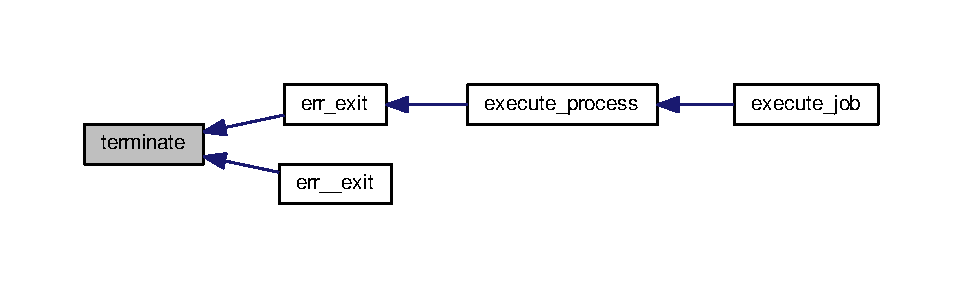
\includegraphics[width=350pt]{err_8c_a8e8952208174427fc9de79dfed72b043_icgraph}
\end{center}
\end{figure}



\hypertarget{err_8h}{\section{src/err.h File Reference}
\label{err_8h}\index{src/err.\-h@{src/err.\-h}}
}


Header file for the error handling subsystem.  


This graph shows which files directly or indirectly include this file\-:\nopagebreak
\begin{figure}[H]
\begin{center}
\leavevmode
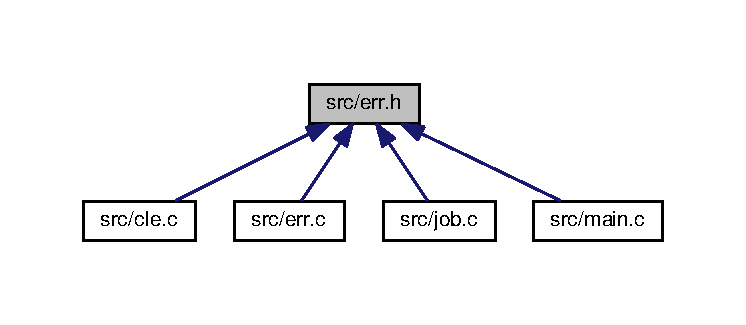
\includegraphics[width=350pt]{err_8h__dep__incl}
\end{center}
\end{figure}
\subsection*{Macros}
\begin{DoxyCompactItemize}
\item 
\#define \hyperlink{err_8h_a40bd4201ea3cf1b6f8e7fef01362bf67}{sfree}(p)~\hyperlink{err_8h_a7a249a2d9b54b1c4c9a43a9d302d637e}{safe\-\_\-free}((void$\ast$$\ast$)\&(p))
\begin{DoxyCompactList}\small\item\em Caller-\/fiendly interface to \hyperlink{err_8h_a7a249a2d9b54b1c4c9a43a9d302d637e}{safe\-\_\-free()}. \end{DoxyCompactList}\item 
\hypertarget{err_8h_aa1728270d73c5d1598de1fd691762eb1}{\#define {\bfseries N\-O\-R\-E\-T\-U\-R\-N}}\label{err_8h_aa1728270d73c5d1598de1fd691762eb1}

\end{DoxyCompactItemize}
\subsection*{Functions}
\begin{DoxyCompactItemize}
\item 
void \hyperlink{err_8h_a7a249a2d9b54b1c4c9a43a9d302d637e}{safe\-\_\-free} (void $\ast$$\ast$pp)
\begin{DoxyCompactList}\small\item\em Safer version of free. \end{DoxyCompactList}\item 
void \hyperlink{err_8h_a07dfb9fd24fe41a9f703bd92af2cf646}{err\-\_\-msg} (const char $\ast$user\-\_\-msg)
\begin{DoxyCompactList}\small\item\em Prints an error message corresponding to the current value of {\itshape errno}. \end{DoxyCompactList}\item 
void \hyperlink{err_8h_a8e8952208174427fc9de79dfed72b043}{terminate} (int use\-\_\-exit3)
\begin{DoxyCompactList}\small\item\em Terminates the calling process. \end{DoxyCompactList}\item 
void \hyperlink{err_8h_abdf2524e566eb527094c786e60c4e15a}{err\-\_\-exit} (const char $\ast$user\-\_\-msg) N\-O\-R\-E\-T\-U\-R\-N
\begin{DoxyCompactList}\small\item\em Prints and error message, and terminates the calling process. \end{DoxyCompactList}\item 
void \hyperlink{err_8h_a30a51bd316b9e22534d7d2c50c110e9e}{err\-\_\-\-\_\-exit} (const char $\ast$user\-\_\-msg) N\-O\-R\-E\-T\-U\-R\-N
\begin{DoxyCompactList}\small\item\em Prints and error message, and terminates the calling process. \end{DoxyCompactList}\end{DoxyCompactItemize}


\subsection{Detailed Description}
Header file for the error handling subsystem. \begin{DoxyAuthor}{Author}
Joe Nathan Abellard \{\href{https://github.com/joenatech7}{\tt https\-://github.\-com/joenatech7}\}
\end{DoxyAuthor}
\begin{DoxyDate}{Date}
September 1, 2017 
\end{DoxyDate}
\begin{DoxyParagraph}{Description}
This file contains function prototypes, and global declarations for the error handing sub system.
\end{DoxyParagraph}
\begin{DoxySeeAlso}{See Also}
\hyperlink{err_8c}{err.\-c} 
\end{DoxySeeAlso}


\subsection{Macro Definition Documentation}
\hypertarget{err_8h_a40bd4201ea3cf1b6f8e7fef01362bf67}{\index{err.\-h@{err.\-h}!sfree@{sfree}}
\index{sfree@{sfree}!err.h@{err.\-h}}
\subsubsection[{sfree}]{\setlength{\rightskip}{0pt plus 5cm}\#define sfree(
\begin{DoxyParamCaption}
\item[{}]{p}
\end{DoxyParamCaption}
)~{\bf safe\-\_\-free}((void$\ast$$\ast$)\&(p))}}\label{err_8h_a40bd4201ea3cf1b6f8e7fef01362bf67}


Caller-\/fiendly interface to \hyperlink{err_8h_a7a249a2d9b54b1c4c9a43a9d302d637e}{safe\-\_\-free()}. 

\begin{DoxyParagraph}{Description}
This macro provides a caller friendly interface to the \hyperlink{err_8h_a7a249a2d9b54b1c4c9a43a9d302d637e}{safe\-\_\-free()} function. By using this marco it is not nessasary to\-: (1) prefix the pointer to the memory block to be allocated with the address of aperator (i.\-e., \&), and (2) to then cast the pointer to void.
\end{DoxyParagraph}
\begin{DoxySeeAlso}{See Also}
\hyperlink{err_8h_a7a249a2d9b54b1c4c9a43a9d302d637e}{safe\-\_\-free()}. 
\end{DoxySeeAlso}


\subsection{Function Documentation}
\hypertarget{err_8h_a30a51bd316b9e22534d7d2c50c110e9e}{\index{err.\-h@{err.\-h}!err\-\_\-\-\_\-exit@{err\-\_\-\-\_\-exit}}
\index{err\-\_\-\-\_\-exit@{err\-\_\-\-\_\-exit}!err.h@{err.\-h}}
\subsubsection[{err\-\_\-\-\_\-exit}]{\setlength{\rightskip}{0pt plus 5cm}void err\-\_\-\-\_\-exit (
\begin{DoxyParamCaption}
\item[{const char $\ast$}]{user\-\_\-msg}
\end{DoxyParamCaption}
)}}\label{err_8h_a30a51bd316b9e22534d7d2c50c110e9e}


Prints and error message, and terminates the calling process. 

\begin{DoxyParagraph}{Description}
This function is used to print an error message and then terminate the calling process. It prints the error message by calling \hyperlink{err_8h_a07dfb9fd24fe41a9f703bd92af2cf646}{err\-\_\-msg()}, and then terminates the process by calling \hyperlink{err_8h_a8e8952208174427fc9de79dfed72b043}{terminate()} wiht the value {\itshape 1} .
\end{DoxyParagraph}

\begin{DoxyParams}{Parameters}
{\em user\-\_\-msg} & This string is passed to \hyperlink{err_8h_a07dfb9fd24fe41a9f703bd92af2cf646}{err\-\_\-msg()}.\\
\hline
\end{DoxyParams}
\begin{DoxyReturn}{Returns}
Returns {\itshape void}.
\end{DoxyReturn}
\begin{DoxySeeAlso}{See Also}
\hyperlink{err_8h_a07dfb9fd24fe41a9f703bd92af2cf646}{err\-\_\-msg()}, \hyperlink{err_8h_a8e8952208174427fc9de79dfed72b043}{terminate()}, and \hyperlink{err_8h_abdf2524e566eb527094c786e60c4e15a}{err\-\_\-exit()}. 
\end{DoxySeeAlso}


Here is the call graph for this function\-:\nopagebreak
\begin{figure}[H]
\begin{center}
\leavevmode
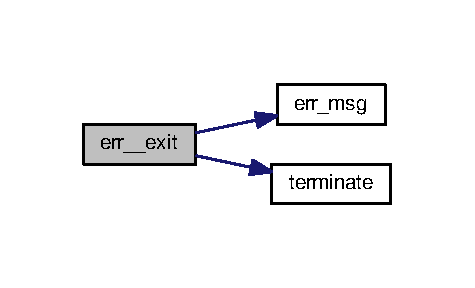
\includegraphics[width=228pt]{err_8h_a30a51bd316b9e22534d7d2c50c110e9e_cgraph}
\end{center}
\end{figure}


\hypertarget{err_8h_abdf2524e566eb527094c786e60c4e15a}{\index{err.\-h@{err.\-h}!err\-\_\-exit@{err\-\_\-exit}}
\index{err\-\_\-exit@{err\-\_\-exit}!err.h@{err.\-h}}
\subsubsection[{err\-\_\-exit}]{\setlength{\rightskip}{0pt plus 5cm}void err\-\_\-exit (
\begin{DoxyParamCaption}
\item[{const char $\ast$}]{user\-\_\-msg}
\end{DoxyParamCaption}
)}}\label{err_8h_abdf2524e566eb527094c786e60c4e15a}


Prints and error message, and terminates the calling process. 

\begin{DoxyParagraph}{Description}
This function is used to print an error message and then terminate the calling process. It prints the error message by calling \hyperlink{err_8h_a07dfb9fd24fe41a9f703bd92af2cf646}{err\-\_\-msg()}, and then terminates the process by calling \hyperlink{err_8h_a8e8952208174427fc9de79dfed72b043}{terminate()} wiht the value {\itshape 0} .
\end{DoxyParagraph}

\begin{DoxyParams}{Parameters}
{\em user\-\_\-msg} & This string is passed to \hyperlink{err_8h_a07dfb9fd24fe41a9f703bd92af2cf646}{err\-\_\-msg()}.\\
\hline
\end{DoxyParams}
\begin{DoxyReturn}{Returns}
Returns {\itshape void}.
\end{DoxyReturn}
\begin{DoxySeeAlso}{See Also}
\hyperlink{err_8h_a07dfb9fd24fe41a9f703bd92af2cf646}{err\-\_\-msg()}, \hyperlink{err_8h_a8e8952208174427fc9de79dfed72b043}{terminate()}, and \hyperlink{err_8h_a30a51bd316b9e22534d7d2c50c110e9e}{err\-\_\-\-\_\-exit()}. 
\end{DoxySeeAlso}


Here is the call graph for this function\-:\nopagebreak
\begin{figure}[H]
\begin{center}
\leavevmode
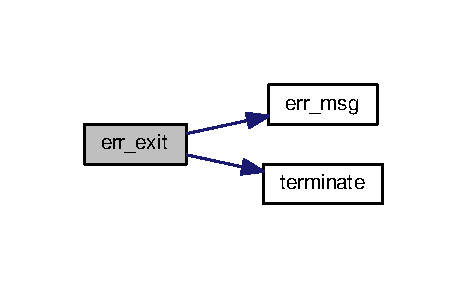
\includegraphics[width=224pt]{err_8h_abdf2524e566eb527094c786e60c4e15a_cgraph}
\end{center}
\end{figure}




Here is the caller graph for this function\-:\nopagebreak
\begin{figure}[H]
\begin{center}
\leavevmode
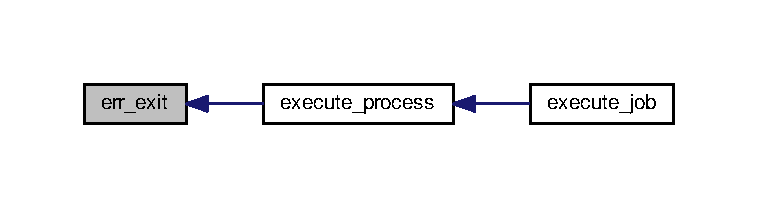
\includegraphics[width=350pt]{err_8h_abdf2524e566eb527094c786e60c4e15a_icgraph}
\end{center}
\end{figure}


\hypertarget{err_8h_a07dfb9fd24fe41a9f703bd92af2cf646}{\index{err.\-h@{err.\-h}!err\-\_\-msg@{err\-\_\-msg}}
\index{err\-\_\-msg@{err\-\_\-msg}!err.h@{err.\-h}}
\subsubsection[{err\-\_\-msg}]{\setlength{\rightskip}{0pt plus 5cm}void err\-\_\-msg (
\begin{DoxyParamCaption}
\item[{const char $\ast$}]{user\-\_\-msg}
\end{DoxyParamCaption}
)}}\label{err_8h_a07dfb9fd24fe41a9f703bd92af2cf646}


Prints an error message corresponding to the current value of {\itshape errno}. 

\begin{DoxyParagraph}{Description}
This function is used to print an error message coresponding to the current value of . It is a more verbose version of the standard {\itshape perror()} function.
\end{DoxyParagraph}

\begin{DoxyParams}{Parameters}
{\em user\-\_\-msg} & This string prefixes the error message that will be printed.\\
\hline
\end{DoxyParams}
\begin{DoxyReturn}{Returns}
Returns {\itshape void}.
\end{DoxyReturn}
\begin{DoxySeeAlso}{See Also}
{\itshape perror()}, {\itshape errno}, {\itshape malloc()}, {\itshape sprintf()}, {\itshape fflush()}, \hyperlink{err_8h_a8e8952208174427fc9de79dfed72b043}{terminate()}, \hyperlink{err_8h_abdf2524e566eb527094c786e60c4e15a}{err\-\_\-exit()}, {\itshape fputs()}, \hyperlink{err_8h_a40bd4201ea3cf1b6f8e7fef01362bf67}{sfree()}, and \hyperlink{err_8h_a30a51bd316b9e22534d7d2c50c110e9e}{err\-\_\-\-\_\-exit()}. 
\end{DoxySeeAlso}


Here is the caller graph for this function\-:\nopagebreak
\begin{figure}[H]
\begin{center}
\leavevmode
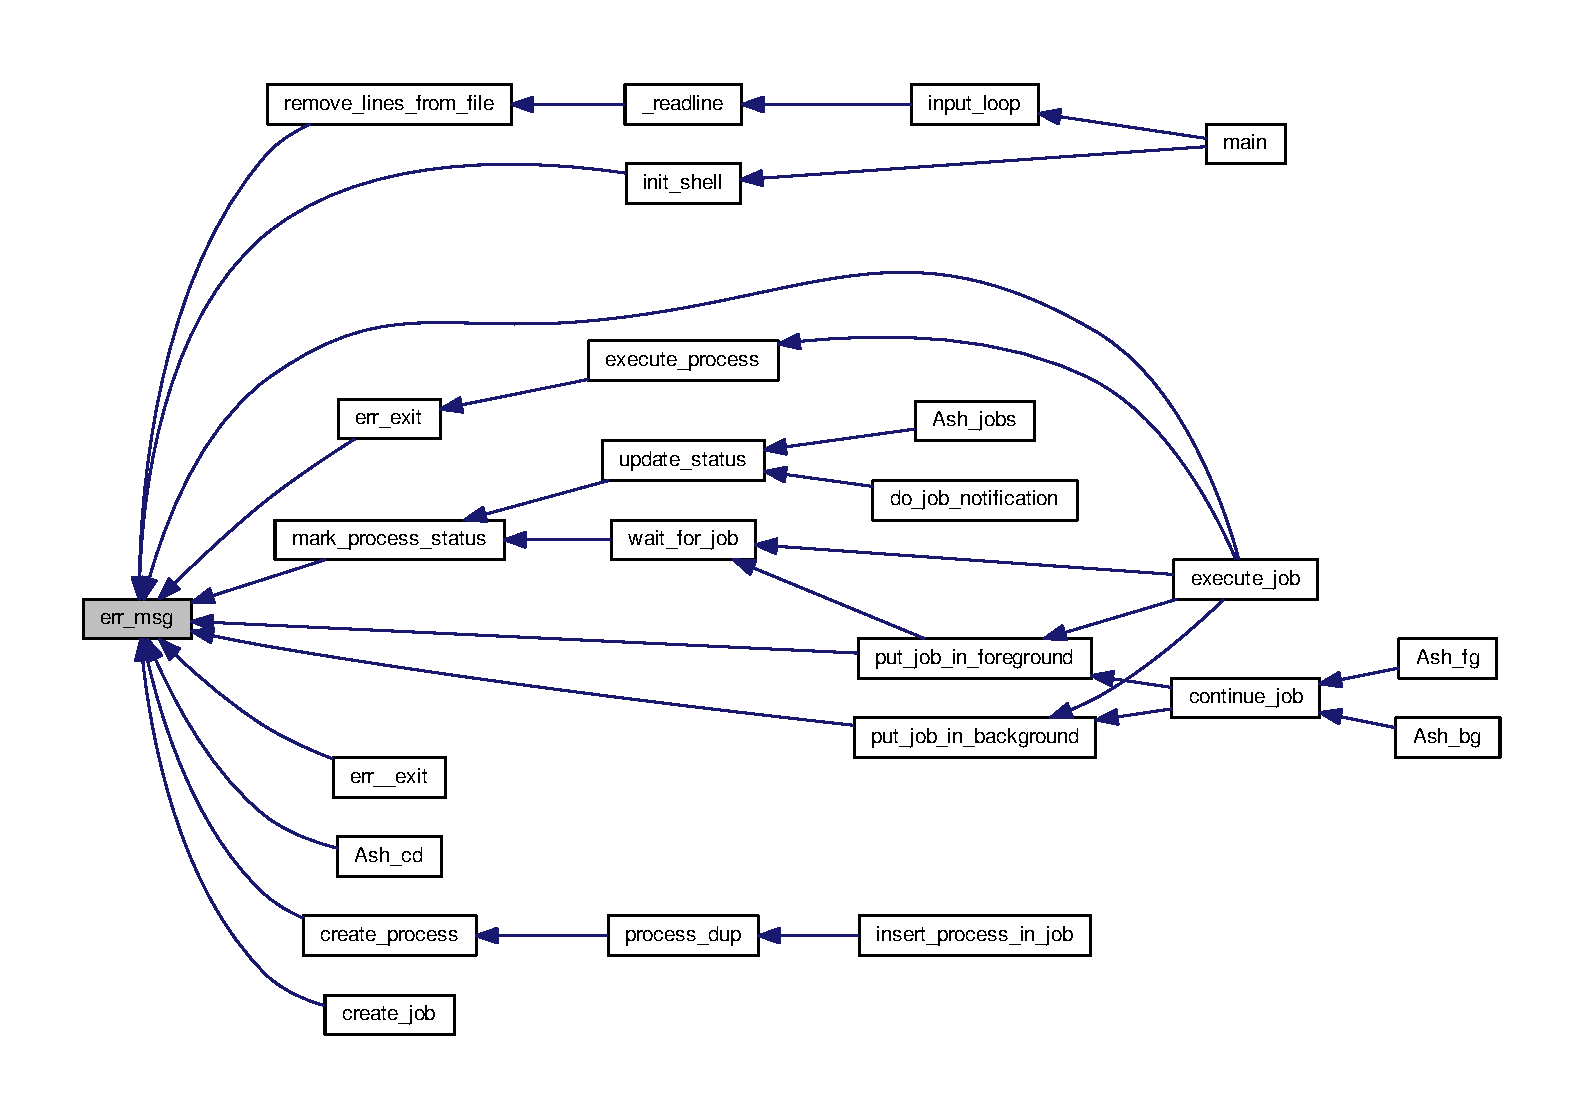
\includegraphics[width=350pt]{err_8h_a07dfb9fd24fe41a9f703bd92af2cf646_icgraph}
\end{center}
\end{figure}


\hypertarget{err_8h_a7a249a2d9b54b1c4c9a43a9d302d637e}{\index{err.\-h@{err.\-h}!safe\-\_\-free@{safe\-\_\-free}}
\index{safe\-\_\-free@{safe\-\_\-free}!err.h@{err.\-h}}
\subsubsection[{safe\-\_\-free}]{\setlength{\rightskip}{0pt plus 5cm}void safe\-\_\-free (
\begin{DoxyParamCaption}
\item[{void $\ast$$\ast$}]{pp}
\end{DoxyParamCaption}
)}}\label{err_8h_a7a249a2d9b54b1c4c9a43a9d302d637e}


Safer version of free. 

\begin{DoxyParagraph}{Description}
This function is a safer version of {\itshape free()}, which is used for de-\/allocating memory from the heap. The are two potential pillfalls when using the standard {\itshape free()} function\-: (1) passing it a N\-U\-L\-L pointer, which results in a run-\/time exeption, and (2) passing it a pointer to a memory block that has already been previously de-\/allocated, resulting in a double free exeption. It is good practice to ensure that (1) a pointer that is to be passed is {\itshape free()} is non-\/\-N\-U\-L\-L, and (2) and to assign N\-U\-L\-L to a pointer right after the memory block it points to has been de-\/allocated with {\itshape free()} . Doing (1) can be inconvinient, and since a pointer is only passed by value to {\itshape free()}, {\itshape free()} can not do (2) on behalf of the programmer. \hyperlink{err_8h_a7a249a2d9b54b1c4c9a43a9d302d637e}{safe\-\_\-free()} seeks to eliminate these inconveniences. It calls {\itshape free()} internally to de-\/allocate memory, but does some things differently than {\itshape free()}. Before calling {\itshape free()} \hyperlink{err_8h_a7a249a2d9b54b1c4c9a43a9d302d637e}{safe\-\_\-free()} checks if the pointer to the momory block is N\-U\-L\-L, and if that is the case, does nothing. Otherwise, it calls {\itshape free()} to de-\/allocate the memory block. It's argument is a pointer to pointer pointing to memory block to be de-\/allocated (i.\-e, a double pointer). Accepting a double pointer allows it to assign N\-U\-L\-L to the pointer after the memory de-\/allocation.
\end{DoxyParagraph}

\begin{DoxyParams}{Parameters}
{\em pp} & Pointer to the pointer pointing to the memory block to be de-\/allocated.\\
\hline
\end{DoxyParams}
\begin{DoxyReturn}{Returns}
returns {\itshape void} 
\end{DoxyReturn}
\begin{DoxySeeAlso}{See Also}
\hyperlink{err_8h_a40bd4201ea3cf1b6f8e7fef01362bf67}{sfree(p)}, and {\itshape free()} 
\end{DoxySeeAlso}
\hypertarget{err_8h_a8e8952208174427fc9de79dfed72b043}{\index{err.\-h@{err.\-h}!terminate@{terminate}}
\index{terminate@{terminate}!err.h@{err.\-h}}
\subsubsection[{terminate}]{\setlength{\rightskip}{0pt plus 5cm}void terminate (
\begin{DoxyParamCaption}
\item[{int}]{use\-\_\-exit3}
\end{DoxyParamCaption}
)}}\label{err_8h_a8e8952208174427fc9de79dfed72b043}


Terminates the calling process. 

\begin{DoxyParagraph}{Description}
This function is used to terminate the calling process. It does that by calling either {\itshape abort()} , {\itshape exit()} , or {\itshape \-\_\-exit()} . If the environment variable E\-F\-\_\-\-D\-U\-M\-P\-C\-O\-R\-E is defined, and is a non-\/empty string, it ends the process by calling {\itshape abort()}. Otherwise the function ends the process by calling either {\itshape exit()} , or {\itshape \-\_\-exit()} .
\end{DoxyParagraph}

\begin{DoxyParams}{Parameters}
{\em use\-\_\-exit3} & This interger determines whether the function calls {\itshape exit()} , or {\itshape \-\_\-exit()} . If it is non-\/zero, it calls {\itshape exit()} with the value E\-X\-I\-T\-\_\-\-F\-A\-I\-L\-U\-R\-E, otherwise it calls {\itshape \-\_\-exit()} with the value E\-X\-I\-T\-\_\-\-F\-A\-I\-L\-U\-R\-E.\\
\hline
\end{DoxyParams}
\begin{DoxyReturn}{Returns}
Returns {\itshape void}.
\end{DoxyReturn}
\begin{DoxySeeAlso}{See Also}
E\-F\-\_\-\-D\-U\-M\-P\-C\-O\-R\-E, {\itshape exit()}, {\itshape \-\_\-exit()}, {\itshape abort()}, \hyperlink{err_8h_a07dfb9fd24fe41a9f703bd92af2cf646}{err\-\_\-msg()}, \hyperlink{err_8h_abdf2524e566eb527094c786e60c4e15a}{err\-\_\-exit()}, E\-X\-I\-T\-\_\-\-F\-A\-I\-L\-U\-R\-E, and \hyperlink{err_8h_a30a51bd316b9e22534d7d2c50c110e9e}{err\-\_\-\-\_\-exit()}. 
\end{DoxySeeAlso}


Here is the caller graph for this function\-:\nopagebreak
\begin{figure}[H]
\begin{center}
\leavevmode
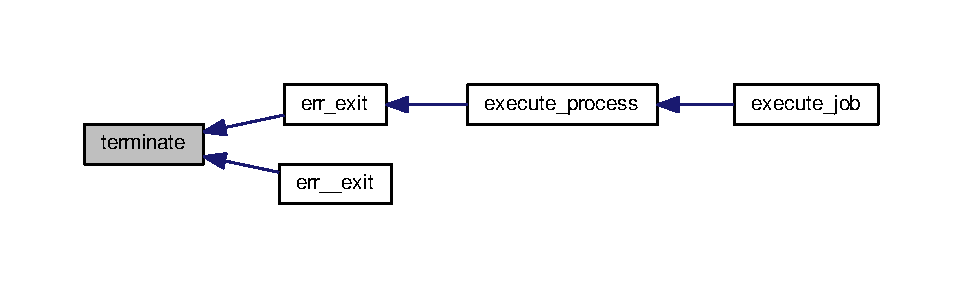
\includegraphics[width=350pt]{err_8h_a8e8952208174427fc9de79dfed72b043_icgraph}
\end{center}
\end{figure}



\hypertarget{job_8c}{\section{src/job.c File Reference}
\label{job_8c}\index{src/job.\-c@{src/job.\-c}}
}


Contains the code for the job control sub system.  


{\ttfamily \#include $<$stdio.\-h$>$}\\*
{\ttfamily \#include $<$stdlib.\-h$>$}\\*
{\ttfamily \#include $<$sys/stat.\-h$>$}\\*
{\ttfamily \#include $<$fcntl.\-h$>$}\\*
{\ttfamily \#include $<$unistd.\-h$>$}\\*
{\ttfamily \#include $<$string.\-h$>$}\\*
{\ttfamily \#include \char`\"{}job.\-h\char`\"{}}\\*
{\ttfamily \#include \char`\"{}err.\-h\char`\"{}}\\*
{\ttfamily \#include $<$signal.\-h$>$}\\*
{\ttfamily \#include $<$errno.\-h$>$}\\*
Include dependency graph for job.\-c\-:\nopagebreak
\begin{figure}[H]
\begin{center}
\leavevmode
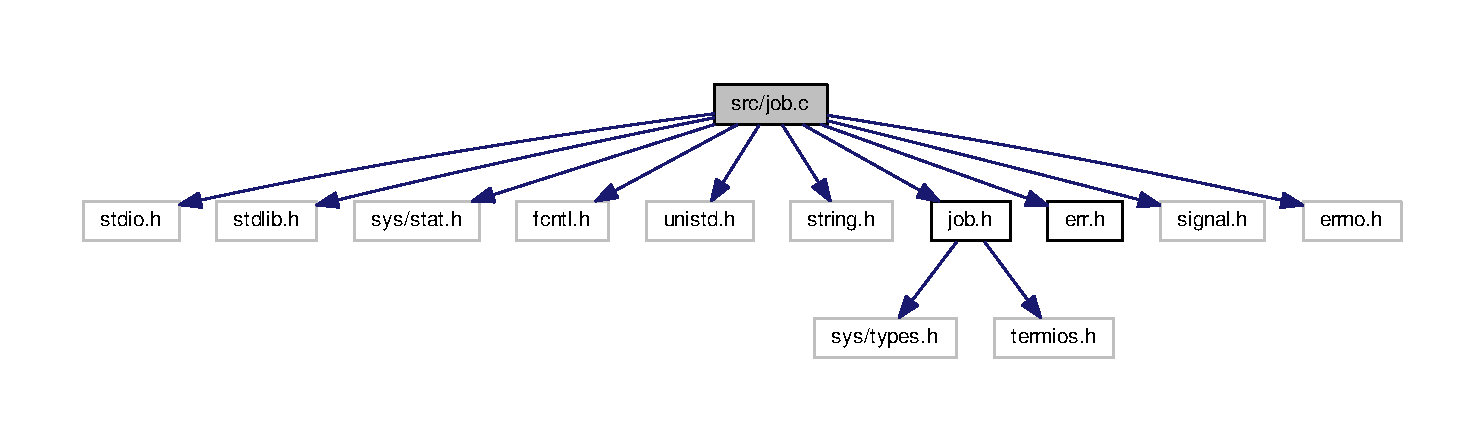
\includegraphics[width=350pt]{job_8c__incl}
\end{center}
\end{figure}
\subsection*{Functions}
\begin{DoxyCompactItemize}
\item 
int \hyperlink{job_8c_a2c2cfa6591ee05cc5bf0c39f38b9e2ea}{Ash\-\_\-cd} (\hyperlink{struct__process}{Process} $\ast$p, int in\-\_\-file, int out\-\_\-file, int err\-\_\-file)
\begin{DoxyCompactList}\small\item\em \mbox{[}B\-U\-I\-L\-T\-I\-N\mbox{]}\-: Changes the shell's current working directory. \end{DoxyCompactList}\item 
int \hyperlink{job_8c_a9fa5abe15df71a688905dc7b29a1389f}{Ash\-\_\-exit} (\hyperlink{struct__process}{Process} $\ast$p, int in\-\_\-file, int out\-\_\-file, int err\-\_\-file)
\begin{DoxyCompactList}\small\item\em \mbox{[}B\-U\-I\-L\-T\-I\-N\mbox{]}\-: Exits from the shell. \end{DoxyCompactList}\item 
int \hyperlink{job_8c_ae54ca57ee056e74d8ae32967453e4482}{print\-\_\-job\-\_\-command} (\hyperlink{struct__job}{Job} $\ast$j, int dest\-\_\-fd)
\begin{DoxyCompactList}\small\item\em Prints the command associated with a job. \end{DoxyCompactList}\item 
int \hyperlink{job_8c_a8950ee4bf84f8322e0b294d0c448a9e7}{Ash\-\_\-jobs} (\hyperlink{struct__process}{Process} $\ast$p, int in\-\_\-file, int out\-\_\-file, int err\-\_\-file)
\begin{DoxyCompactList}\small\item\em \mbox{[}B\-U\-I\-L\-T\-I\-N\mbox{]}\-: List the jobs in the shell's active job list. \end{DoxyCompactList}\item 
int \hyperlink{job_8c_a792fcc9814d020b087911591c5fce10b}{Ash\-\_\-fg} (\hyperlink{struct__process}{Process} $\ast$p, int in\-\_\-file, int out\-\_\-file, int err\-\_\-file)
\begin{DoxyCompactList}\small\item\em \mbox{[}B\-U\-I\-L\-T\-I\-N\mbox{]}\-: Continues an active job in the foreground. \end{DoxyCompactList}\item 
int \hyperlink{job_8c_a9bc6f26d0ab14359707a0f367f1a6522}{Ash\-\_\-bg} (\hyperlink{struct__process}{Process} $\ast$p, int in\-\_\-file, int out\-\_\-file, int err\-\_\-file)
\begin{DoxyCompactList}\small\item\em \mbox{[}B\-U\-I\-L\-T\-I\-N\mbox{]}\-: Continues active jobs in the background. \end{DoxyCompactList}\item 
int \hyperlink{job_8c_a4242d3cdbc0468d774243dc67b330296}{Ash\-\_\-help} (\hyperlink{struct__process}{Process} $\ast$p, int in\-\_\-file, int out\-\_\-file, int err\-\_\-file)
\begin{DoxyCompactList}\small\item\em \mbox{[}B\-U\-I\-L\-T\-I\-N\mbox{]}\-: Prints a help message for the shell. \end{DoxyCompactList}\item 
int \hyperlink{job_8c_a723e6648fca47a139cdff5cf4f1bc4bb}{Ash\-\_\-kill} (\hyperlink{struct__process}{Process} $\ast$p, int in\-\_\-file, int out\-\_\-file, int err\-\_\-file)
\begin{DoxyCompactList}\small\item\em \mbox{[}B\-U\-I\-L\-T\-I\-N\mbox{]}\-: Sends a signal to active jobs. \end{DoxyCompactList}\item 
int \hyperlink{job_8c_a07e5c62e1d5e55012cf188dd32b6cf27}{Ash\-\_\-killall} (\hyperlink{struct__process}{Process} $\ast$p, int in\-\_\-file, int out\-\_\-file, int err\-\_\-file)
\begin{DoxyCompactList}\small\item\em \mbox{[}B\-U\-I\-L\-T\-I\-N\mbox{]}\-: Sends a signal to all active jobs. \end{DoxyCompactList}\item 
int \hyperlink{job_8c_a028aee0dd87474ee61f6c654efe653a2}{is\-\_\-builtin} (\hyperlink{struct__process}{Process} $\ast$p)
\begin{DoxyCompactList}\small\item\em \mbox{[}B\-U\-I\-L\-T\-I\-N\mbox{]}\-: Checks if a command refers to a shell builtin. \end{DoxyCompactList}\item 
void \hyperlink{job_8c_a3a5b33cdd8fb591704c9adfcf908a273}{init\-\_\-shell} ()
\begin{DoxyCompactList}\small\item\em Initializes the shell. \end{DoxyCompactList}\item 
\hyperlink{struct__process}{Process} $\ast$ \hyperlink{job_8c_a1af7ca10dbe6b9358262cc18f04bf6f5}{create\-\_\-process} (void)
\begin{DoxyCompactList}\small\item\em Creates an instance of a process. \end{DoxyCompactList}\item 
int \hyperlink{job_8c_ad5ee9895c47b901c083c541e8f021abe}{insert\-\_\-arg\-\_\-in\-\_\-process} (\hyperlink{struct__process}{Process} $\ast$p, const char $\ast$arg)
\begin{DoxyCompactList}\small\item\em Inserts an argument in the argument vector of a process. \end{DoxyCompactList}\item 
void \hyperlink{job_8c_a8226a1a322fce279b7510ee28c09f40e}{print\-\_\-process} (const \hyperlink{struct__process}{Process} $\ast$p)
\begin{DoxyCompactList}\small\item\em Prints the command of a process. \end{DoxyCompactList}\item 
\hyperlink{struct__process}{Process} $\ast$ \hyperlink{job_8c_a9c2d0895268bd3229fc231b00029eb7b}{process\-\_\-dup} (const \hyperlink{struct__process}{Process} $\ast$p)
\begin{DoxyCompactList}\small\item\em Duplicates an instance of a process. \end{DoxyCompactList}\item 
void \hyperlink{job_8c_acaa6f75b768f52660498b9fab3898e15}{execute\-\_\-process} (\hyperlink{struct__process}{Process} $\ast$p, pid\-\_\-t pgid, int in\-\_\-file, int out\-\_\-file, int err\-\_\-file, int foreground)
\begin{DoxyCompactList}\small\item\em Executes a process. \end{DoxyCompactList}\item 
void \hyperlink{job_8c_a167097d11d4b3ceda7957cb5244de3a8}{destroy\-\_\-process} (\hyperlink{struct__process}{Process} $\ast$p)
\begin{DoxyCompactList}\small\item\em Destroys a process instance. \end{DoxyCompactList}\item 
\hyperlink{struct__job}{Job} $\ast$ \hyperlink{job_8c_a18d3d13da14c1f38fa2b0932e8850129}{create\-\_\-job} (void)
\begin{DoxyCompactList}\small\item\em Creates a new job instance. \end{DoxyCompactList}\item 
int \hyperlink{job_8c_a78dbe5452200ef69f412085af895096b}{insert\-\_\-process\-\_\-in\-\_\-job} (\hyperlink{struct__job}{Job} $\ast$j, const \hyperlink{struct__process}{Process} $\ast$p)
\begin{DoxyCompactList}\small\item\em Inserts a process instance in a job instance. \end{DoxyCompactList}\item 
void \hyperlink{job_8c_a89462129d286d10ccab2bd69e70ac336}{print\-\_\-job} (const \hyperlink{struct__job}{Job} $\ast$j)
\begin{DoxyCompactList}\small\item\em Prints a job. \end{DoxyCompactList}\item 
int \hyperlink{job_8c_a8c729ad459ad99d7a0e3c7a549d98383}{destroy\-\_\-job} (\hyperlink{struct__job}{Job} $\ast$j)
\begin{DoxyCompactList}\small\item\em Destroys a job. \end{DoxyCompactList}\item 
\hyperlink{struct__job}{Job} $\ast$ \hyperlink{job_8c_abbd710ae6b1b777643ee31ccac51c985}{find\-\_\-job} (pid\-\_\-t pgid)
\begin{DoxyCompactList}\small\item\em Finds a job with a particular P\-G\-I\-D. \end{DoxyCompactList}\item 
\hyperlink{struct__job}{Job} $\ast$ \hyperlink{job_8c_a870c6d70cfb180e88d217a0b3501aedb}{find\-\_\-job\-\_\-id} (int id)
\begin{DoxyCompactList}\small\item\em Finds a job with a particular I\-D. \end{DoxyCompactList}\item 
int \hyperlink{job_8c_a4b49892bffa5095eb5a0fb7d86659456}{job\-\_\-is\-\_\-stopped} (\hyperlink{struct__job}{Job} $\ast$j)
\begin{DoxyCompactList}\small\item\em Determines if a job is stopped. \end{DoxyCompactList}\item 
int \hyperlink{job_8c_a0654ba7330ec47c1e636afe60657651b}{job\-\_\-is\-\_\-completed} (\hyperlink{struct__job}{Job} $\ast$j)
\begin{DoxyCompactList}\small\item\em Determines if a job is completed. \end{DoxyCompactList}\item 
void \hyperlink{job_8c_ae7a22fe41ac695db73564a23ce25cf6a}{format\-\_\-job\-\_\-info} (\hyperlink{struct__job}{Job} $\ast$j, const char $\ast$status)
\begin{DoxyCompactList}\small\item\em Formats and prints info for a job. \end{DoxyCompactList}\item 
int \hyperlink{job_8c_a5419d481fca1c4c7bb7c89e38b964fa9}{mark\-\_\-process\-\_\-status} (pid\-\_\-t pid, int status)
\begin{DoxyCompactList}\small\item\em Marks the status of a stopped or terminated child process. \end{DoxyCompactList}\item 
void \hyperlink{job_8c_ad8e58b77db46018eeb20c68855538f35}{update\-\_\-status} (void)
\begin{DoxyCompactList}\small\item\em Updates the status of stopped or completed child processes of the shell. \end{DoxyCompactList}\item 
void \hyperlink{job_8c_aead235b523c076d6346ba285fa98f6d1}{wait\-\_\-for\-\_\-job} (\hyperlink{struct__job}{Job} $\ast$j)
\begin{DoxyCompactList}\small\item\em waits for a job to stop or complete. \end{DoxyCompactList}\item 
void \hyperlink{job_8c_a75430387f345a954b011547bf14a56ce}{do\-\_\-job\-\_\-notification} (void)
\begin{DoxyCompactList}\small\item\em Notifies the user of job status updates. \end{DoxyCompactList}\item 
void \hyperlink{job_8c_ab3b7803e9a87944a86267abc40fe6c39}{put\-\_\-job\-\_\-in\-\_\-foreground} (\hyperlink{struct__job}{Job} $\ast$j, int cont)
\begin{DoxyCompactList}\small\item\em Puts a job in the foreground. \end{DoxyCompactList}\item 
void \hyperlink{job_8c_a095ab07b063dbbc25fd2729125fb530a}{put\-\_\-job\-\_\-in\-\_\-background} (\hyperlink{struct__job}{Job} $\ast$j, int cont)
\begin{DoxyCompactList}\small\item\em Puts a job in the background. \end{DoxyCompactList}\item 
void \hyperlink{job_8c_a690fc87028fe2334113ee8d92f8c8f24}{mark\-\_\-job\-\_\-as\-\_\-running} (\hyperlink{struct__job}{Job} $\ast$j)
\begin{DoxyCompactList}\small\item\em Updates a job's state to {\itshape Running} . \end{DoxyCompactList}\item 
void \hyperlink{job_8c_ab69ad21398604a048a5a1b4ef7af1320}{continue\-\_\-job} (\hyperlink{struct__job}{Job} $\ast$j, int foreground)
\begin{DoxyCompactList}\small\item\em Continues a job. \end{DoxyCompactList}\item 
void \hyperlink{job_8c_aff64d308dd49d9da9f2d6f993346f7ad}{add\-\_\-job\-\_\-to\-\_\-list} (\hyperlink{struct__job}{Job} $\ast$j)
\begin{DoxyCompactList}\small\item\em Adds a job to the active job list. \end{DoxyCompactList}\item 
int \hyperlink{job_8c_a328634c49391a29ef1d4e86d6bf0ea7e}{execute\-\_\-job} (\hyperlink{struct__job}{Job} $\ast$j)
\item 
void \hyperlink{job_8c_a4ae3063920907216e6ba0bdc83ac5b15}{print\-\_\-job\-\_\-list} (void)
\begin{DoxyCompactList}\small\item\em Prints the I\-D of jobs in the active job list. \end{DoxyCompactList}\end{DoxyCompactItemize}
\subsection*{Variables}
\begin{DoxyCompactItemize}
\item 
pid\-\_\-t \hyperlink{job_8c_a9dfc260b67728b41e7120b47d7758053}{Ash\-\_\-pgid}
\begin{DoxyCompactList}\small\item\em Process group I\-D of the shell. \end{DoxyCompactList}\item 
struct termios \hyperlink{job_8c_a01959f896d957ce001a3a87fc034a5be}{Ash\-\_\-tmodes}
\begin{DoxyCompactList}\small\item\em Default terminal modes of the shell. \end{DoxyCompactList}\item 
int \hyperlink{job_8c_a079811c5e88059665d23821b4a38802a}{Ash\-\_\-terminal}
\begin{DoxyCompactList}\small\item\em File descriptor to standard input for the shell. \end{DoxyCompactList}\item 
int \hyperlink{job_8c_af7730a56d05055a70f3c18ee938209f8}{Ash\-\_\-is\-\_\-interactive}
\begin{DoxyCompactList}\small\item\em Indicates if the shell is running interactively. \end{DoxyCompactList}\item 
\hyperlink{struct__job}{Job} $\ast$ \hyperlink{job_8c_a4ca397eaae80b0004f61dad81729c06d}{job\-\_\-list\-\_\-head} = N\-U\-L\-L
\begin{DoxyCompactList}\small\item\em Head of the job list. \end{DoxyCompactList}\item 
char $\ast$ \hyperlink{job_8c_a1a6160b9abc239f381d9ba30d00b4e0d}{job\-\_\-states} \mbox{[}$\,$\mbox{]}
\begin{DoxyCompactList}\small\item\em Job state strings. \end{DoxyCompactList}\item 
\hyperlink{job_8h_a165885ac9a829b970ba29594fec5acd7}{Builtin} \hyperlink{job_8c_a2c5551422426f406568d84844b40acb9}{builtins} \mbox{[}$\,$\mbox{]}
\begin{DoxyCompactList}\small\item\em List of shell builtins an associated function. \end{DoxyCompactList}\end{DoxyCompactItemize}


\subsection{Detailed Description}
Contains the code for the job control sub system. \begin{DoxyAuthor}{Author}
Joe Nathan Abellard \{\href{https://github.com/joenatech7}{\tt https\-://github.\-com/joenatech7}\}
\end{DoxyAuthor}
\begin{DoxyDate}{Date}
September 1, 2017 
\end{DoxyDate}
\begin{DoxyParagraph}{Description}
This file contains contains the code for the job control sub system.
\end{DoxyParagraph}
\begin{DoxySeeAlso}{See Also}
\hyperlink{job_8h}{job.\-h} 
\end{DoxySeeAlso}


\subsection{Function Documentation}
\hypertarget{job_8c_aff64d308dd49d9da9f2d6f993346f7ad}{\index{job.\-c@{job.\-c}!add\-\_\-job\-\_\-to\-\_\-list@{add\-\_\-job\-\_\-to\-\_\-list}}
\index{add\-\_\-job\-\_\-to\-\_\-list@{add\-\_\-job\-\_\-to\-\_\-list}!job.c@{job.\-c}}
\subsubsection[{add\-\_\-job\-\_\-to\-\_\-list}]{\setlength{\rightskip}{0pt plus 5cm}void add\-\_\-job\-\_\-to\-\_\-list (
\begin{DoxyParamCaption}
\item[{{\bf Job} $\ast$}]{j}
\end{DoxyParamCaption}
)}}\label{job_8c_aff64d308dd49d9da9f2d6f993346f7ad}


Adds a job to the active job list. 

\begin{DoxyParagraph}{Description}
This function is used to add a job to the end of the linked list (\hyperlink{job_8c_a4ca397eaae80b0004f61dad81729c06d}{job\-\_\-list\-\_\-head}) used to maintain active job records.
\end{DoxyParagraph}

\begin{DoxyParams}{Parameters}
{\em j} & The job to add to the active job list.\\
\hline
\end{DoxyParams}
\begin{DoxyReturn}{Returns}
Returns {\itshape void} .
\end{DoxyReturn}
\begin{DoxySeeAlso}{See Also}
\hyperlink{struct__job}{\-\_\-job}, \hyperlink{job_8c_a4ca397eaae80b0004f61dad81729c06d}{job\-\_\-list\-\_\-head}, and \hyperlink{job_8h_a328634c49391a29ef1d4e86d6bf0ea7e}{execute\-\_\-job()}. 
\end{DoxySeeAlso}


Here is the caller graph for this function\-:\nopagebreak
\begin{figure}[H]
\begin{center}
\leavevmode
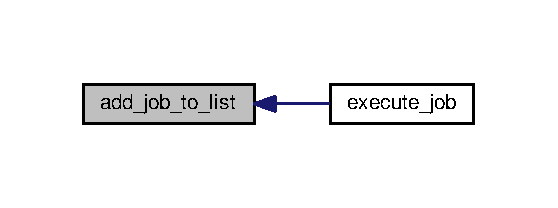
\includegraphics[width=268pt]{job_8c_aff64d308dd49d9da9f2d6f993346f7ad_icgraph}
\end{center}
\end{figure}


\hypertarget{job_8c_a9bc6f26d0ab14359707a0f367f1a6522}{\index{job.\-c@{job.\-c}!Ash\-\_\-bg@{Ash\-\_\-bg}}
\index{Ash\-\_\-bg@{Ash\-\_\-bg}!job.c@{job.\-c}}
\subsubsection[{Ash\-\_\-bg}]{\setlength{\rightskip}{0pt plus 5cm}int Ash\-\_\-bg (
\begin{DoxyParamCaption}
\item[{{\bf Process} $\ast$}]{p, }
\item[{int}]{in\-\_\-file, }
\item[{int}]{out\-\_\-file, }
\item[{int}]{err\-\_\-file}
\end{DoxyParamCaption}
)}}\label{job_8c_a9bc6f26d0ab14359707a0f367f1a6522}


\mbox{[}B\-U\-I\-L\-T\-I\-N\mbox{]}\-: Continues active jobs in the background. 

\begin{DoxyParagraph}{Description}
This shell builtin is used to continue active jobs (\hyperlink{struct__job}{\-\_\-job}) in the background. It accepts the following grammar \-: \par
bg -\/$<$job-\/id$>$ ... \par
To continue the job(s) in the background, it does the following \-: \begin{DoxyItemize}
\item Checks if the command grammer is valid. \item If the grammar is valid, then for each job, it calls \hyperlink{job_8h_a870c6d70cfb180e88d217a0b3501aedb}{find\-\_\-job\-\_\-id()} to find the specified jobs on the active job list (job\-\_\-list\-\_\-head) with job I\-D (\-\_\-job\-::id) {\itshape $<$job-\/id$>$} . \item For each job that is found, it calls \hyperlink{job_8h_ab69ad21398604a048a5a1b4ef7af1320}{continue\-\_\-job()} to continue the job in the background.\end{DoxyItemize}

\end{DoxyParagraph}

\begin{DoxyParams}{Parameters}
{\em p} & This is a process (\hyperlink{struct__process}{\-\_\-process}) . Only its argument vector (\-\_\-process\-::argv) and argument count (\-\_\-process\-::argc) are of interest to this builtin.\\
\hline
{\em in\-\_\-file} & File descriptor to the builtin's standard input.\\
\hline
{\em out\-\_\-file} & File descriptor to the builtin's standard output.\\
\hline
{\em in\-\_\-file} & File descriptor to the builtin's standard error.\\
\hline
\end{DoxyParams}
\begin{DoxyReturn}{Returns}
Returns {\itshape 0} on success, or {\itshape -\/1} on error. Possible reasons for failure are as follows\-: \begin{DoxyItemize}
\item The grammar of the command is invalid. \item The grammar of the command is valid, but a specified {\itshape $<$job-\/id$>$} does not refer to a job on the active job list.\end{DoxyItemize}

\end{DoxyReturn}
\begin{DoxySeeAlso}{See Also}
\hyperlink{struct__process}{\-\_\-process}, \-\_\-process\-::argv, \-\_\-process\-::argc, {\itshape dprintf()}, {\itshape atoi()}, \hyperlink{struct__job}{\-\_\-job}, \hyperlink{job_8h_a870c6d70cfb180e88d217a0b3501aedb}{find\-\_\-job\-\_\-id()}, \hyperlink{job_8h_ab69ad21398604a048a5a1b4ef7af1320}{continue\-\_\-job()}, {\itshape strlen()}, (\hyperlink{job_8c_a4ca397eaae80b0004f61dad81729c06d}{job\-\_\-list\-\_\-head}) \hyperlink{job_8h_a2c2cfa6591ee05cc5bf0c39f38b9e2ea}{Ash\-\_\-cd()}, \hyperlink{job_8h_a9fa5abe15df71a688905dc7b29a1389f}{Ash\-\_\-exit()}, \hyperlink{job_8h_a8950ee4bf84f8322e0b294d0c448a9e7}{Ash\-\_\-jobs()}, \hyperlink{job_8h_a9bc6f26d0ab14359707a0f367f1a6522}{Ash\-\_\-bg()}, \hyperlink{job_8h_a4242d3cdbc0468d774243dc67b330296}{Ash\-\_\-help()}, \hyperlink{job_8h_a723e6648fca47a139cdff5cf4f1bc4bb}{Ash\-\_\-kill()}, and \hyperlink{job_8h_a07e5c62e1d5e55012cf188dd32b6cf27}{Ash\-\_\-killall()} 
\end{DoxySeeAlso}


Here is the call graph for this function\-:\nopagebreak
\begin{figure}[H]
\begin{center}
\leavevmode
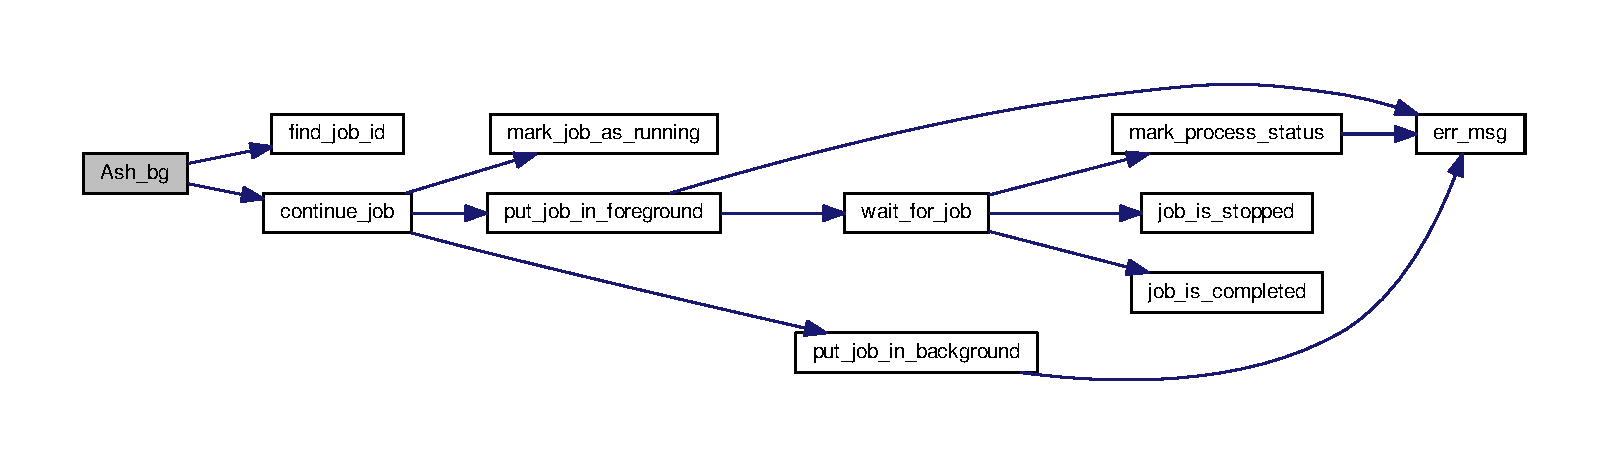
\includegraphics[width=350pt]{job_8c_a9bc6f26d0ab14359707a0f367f1a6522_cgraph}
\end{center}
\end{figure}


\hypertarget{job_8c_a2c2cfa6591ee05cc5bf0c39f38b9e2ea}{\index{job.\-c@{job.\-c}!Ash\-\_\-cd@{Ash\-\_\-cd}}
\index{Ash\-\_\-cd@{Ash\-\_\-cd}!job.c@{job.\-c}}
\subsubsection[{Ash\-\_\-cd}]{\setlength{\rightskip}{0pt plus 5cm}int Ash\-\_\-cd (
\begin{DoxyParamCaption}
\item[{{\bf Process} $\ast$}]{p, }
\item[{int}]{in\-\_\-file, }
\item[{int}]{out\-\_\-file, }
\item[{int}]{err\-\_\-file}
\end{DoxyParamCaption}
)}}\label{job_8c_a2c2cfa6591ee05cc5bf0c39f38b9e2ea}


\mbox{[}B\-U\-I\-L\-T\-I\-N\mbox{]}\-: Changes the shell's current working directory. 

\begin{DoxyParagraph}{Description}
This shell builtin is used to change the shell's current working directory. It accepts the following grammar \-: \par
cd $<$path-\/to-\/new-\/direcotry$>$ \par
To change the current working directory, it does the following \-: \begin{DoxyItemize}
\item Checks if the grammar of the command is correct. \item If the grammar of the command is correct, the function calls {\itshape chdir()} to change the current working directory.\end{DoxyItemize}

\end{DoxyParagraph}

\begin{DoxyParams}{Parameters}
{\em p} & This is a process (\hyperlink{struct__process}{\-\_\-process}) . Only its argument vector (\-\_\-process\-::argv) and argument count (\-\_\-process\-::argc) fields are of interest for the builtin.\\
\hline
{\em in\-\_\-file} & File descriptor to the builtin's standard input.\\
\hline
{\em out\-\_\-file} & File descriptor to the builtin's standard output.\\
\hline
{\em in\-\_\-file} & File descriptor to the builtin's standard error.\\
\hline
\end{DoxyParams}
\begin{DoxyReturn}{Returns}
Returns {\itshape 0} on success, or {\itshape -\/1} on failure. Possible reasons for failure are as follows\-: \begin{DoxyItemize}
\item The grammar passed to the builtin is invalid. \item The call to {\itshape chdir()} fails\end{DoxyItemize}

\end{DoxyReturn}
\begin{DoxySeeAlso}{See Also}
\hyperlink{struct__process}{\-\_\-process}, \-\_\-process\-::argv, \-\_\-process\-::argc, {\itshape chdir()} , \hyperlink{err_8c_a07dfb9fd24fe41a9f703bd92af2cf646}{err\-\_\-msg()}, {\itshape dprintf()}, \hyperlink{job_8h_a9fa5abe15df71a688905dc7b29a1389f}{Ash\-\_\-exit()}, \hyperlink{job_8h_a8950ee4bf84f8322e0b294d0c448a9e7}{Ash\-\_\-jobs()}, \hyperlink{job_8h_a792fcc9814d020b087911591c5fce10b}{Ash\-\_\-fg()}, \hyperlink{job_8h_a9bc6f26d0ab14359707a0f367f1a6522}{Ash\-\_\-bg()}, \hyperlink{job_8h_a4242d3cdbc0468d774243dc67b330296}{Ash\-\_\-help()}, \hyperlink{job_8h_a723e6648fca47a139cdff5cf4f1bc4bb}{Ash\-\_\-kill()}, and \hyperlink{job_8h_a07e5c62e1d5e55012cf188dd32b6cf27}{Ash\-\_\-killall()}. 
\end{DoxySeeAlso}


Here is the call graph for this function\-:\nopagebreak
\begin{figure}[H]
\begin{center}
\leavevmode
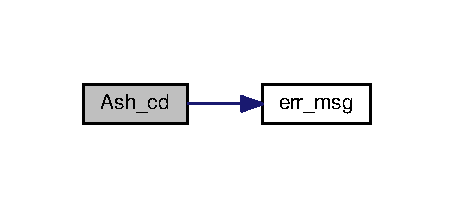
\includegraphics[width=218pt]{job_8c_a2c2cfa6591ee05cc5bf0c39f38b9e2ea_cgraph}
\end{center}
\end{figure}


\hypertarget{job_8c_a9fa5abe15df71a688905dc7b29a1389f}{\index{job.\-c@{job.\-c}!Ash\-\_\-exit@{Ash\-\_\-exit}}
\index{Ash\-\_\-exit@{Ash\-\_\-exit}!job.c@{job.\-c}}
\subsubsection[{Ash\-\_\-exit}]{\setlength{\rightskip}{0pt plus 5cm}int Ash\-\_\-exit (
\begin{DoxyParamCaption}
\item[{{\bf Process} $\ast$}]{p, }
\item[{int}]{in\-\_\-file, }
\item[{int}]{out\-\_\-file, }
\item[{int}]{err\-\_\-file}
\end{DoxyParamCaption}
)}}\label{job_8c_a9fa5abe15df71a688905dc7b29a1389f}


\mbox{[}B\-U\-I\-L\-T\-I\-N\mbox{]}\-: Exits from the shell. 

\begin{DoxyParagraph}{Description}
This shell builtin is used exit from the shell. It accepts the following grammar \-: \par
exit \par
To exit from the shell, it does the following \-: \begin{DoxyItemize}
\item calls () with the status E\-X\-I\-T\-\_\-\-S\-U\-C\-C\-E\-S\-S.\end{DoxyItemize}

\end{DoxyParagraph}

\begin{DoxyParams}{Parameters}
{\em p} & This is a process (\hyperlink{struct__process}{\-\_\-process}) . It is not of interest to this builtin.\\
\hline
{\em in\-\_\-file} & File descriptor to the builtin's standard input.\\
\hline
{\em out\-\_\-file} & File descriptor to the builtin's standard output.\\
\hline
{\em in\-\_\-file} & File descriptor to the builtin's standard error.\\
\hline
\end{DoxyParams}
\begin{DoxyReturn}{Returns}
Never returns.
\end{DoxyReturn}
\begin{DoxySeeAlso}{See Also}
\hyperlink{struct__process}{\-\_\-process}, {\itshape exit()}, \hyperlink{job_8h_a2c2cfa6591ee05cc5bf0c39f38b9e2ea}{Ash\-\_\-cd()}, \hyperlink{job_8h_a8950ee4bf84f8322e0b294d0c448a9e7}{Ash\-\_\-jobs()}, \hyperlink{job_8h_a792fcc9814d020b087911591c5fce10b}{Ash\-\_\-fg()}, \hyperlink{job_8h_a9bc6f26d0ab14359707a0f367f1a6522}{Ash\-\_\-bg()}, \hyperlink{job_8h_a4242d3cdbc0468d774243dc67b330296}{Ash\-\_\-help()}, \hyperlink{job_8h_a723e6648fca47a139cdff5cf4f1bc4bb}{Ash\-\_\-kill()}, and \hyperlink{job_8h_a07e5c62e1d5e55012cf188dd32b6cf27}{Ash\-\_\-killall()} 
\end{DoxySeeAlso}
\hypertarget{job_8c_a792fcc9814d020b087911591c5fce10b}{\index{job.\-c@{job.\-c}!Ash\-\_\-fg@{Ash\-\_\-fg}}
\index{Ash\-\_\-fg@{Ash\-\_\-fg}!job.c@{job.\-c}}
\subsubsection[{Ash\-\_\-fg}]{\setlength{\rightskip}{0pt plus 5cm}int Ash\-\_\-fg (
\begin{DoxyParamCaption}
\item[{{\bf Process} $\ast$}]{p, }
\item[{int}]{in\-\_\-file, }
\item[{int}]{out\-\_\-file, }
\item[{int}]{err\-\_\-file}
\end{DoxyParamCaption}
)}}\label{job_8c_a792fcc9814d020b087911591c5fce10b}


\mbox{[}B\-U\-I\-L\-T\-I\-N\mbox{]}\-: Continues an active job in the foreground. 

\begin{DoxyParagraph}{Description}
This shell builtin is used to continue an active job (\hyperlink{struct__job}{\-\_\-job}) in the foreground. It accepts the following grammar \-: \par
fg -\/$<$job-\/id$>$ \par
To continue the job in the foreground, it does the following \-: \begin{DoxyItemize}
\item Checks if the command grammer is valid. \item If the grammar is valid, it calls \hyperlink{job_8h_a870c6d70cfb180e88d217a0b3501aedb}{find\-\_\-job\-\_\-id()} to find a job on the active job list (job\-\_\-list\-\_\-head) with job I\-D (\-\_\-job\-::id) {\itshape $<$job-\/id$>$} . \item If it finds the job, it calls \hyperlink{job_8h_ab69ad21398604a048a5a1b4ef7af1320}{continue\-\_\-job()} to continue the job in the foreground.\end{DoxyItemize}

\end{DoxyParagraph}

\begin{DoxyParams}{Parameters}
{\em p} & This is a process (\hyperlink{struct__process}{\-\_\-process}) . Only its argument vector (\-\_\-process\-::argv) and argument count (\-\_\-process\-::argc) are of interest to this builtin.\\
\hline
{\em in\-\_\-file} & File descriptor to the builtin's standard input.\\
\hline
{\em out\-\_\-file} & File descriptor to the builtin's standard output.\\
\hline
{\em in\-\_\-file} & File descriptor to the builtin's standard error.\\
\hline
\end{DoxyParams}
\begin{DoxyReturn}{Returns}
Returns {\itshape 0} on success, or {\itshape -\/1} on error. Possible reasons for failure are as follows\-: \begin{DoxyItemize}
\item The grammar of the command is invalid. \item The grammar of the command is valid, but {\itshape $<$job-\/id$>$} does not refer to a job on the active job list.\end{DoxyItemize}

\end{DoxyReturn}
\begin{DoxySeeAlso}{See Also}
\hyperlink{struct__process}{\-\_\-process}, \-\_\-process\-::argv, \-\_\-process\-::argc, {\itshape dprintf()}, {\itshape atoi()}, \hyperlink{struct__job}{\-\_\-job}, \hyperlink{job_8h_a870c6d70cfb180e88d217a0b3501aedb}{find\-\_\-job\-\_\-id()}, \hyperlink{job_8h_ab69ad21398604a048a5a1b4ef7af1320}{continue\-\_\-job()}, \hyperlink{job_8h_a2c2cfa6591ee05cc5bf0c39f38b9e2ea}{Ash\-\_\-cd()}, \hyperlink{job_8h_a9fa5abe15df71a688905dc7b29a1389f}{Ash\-\_\-exit()}, \hyperlink{job_8h_a8950ee4bf84f8322e0b294d0c448a9e7}{Ash\-\_\-jobs()}, \hyperlink{job_8h_a9bc6f26d0ab14359707a0f367f1a6522}{Ash\-\_\-bg()}, \hyperlink{job_8h_a4242d3cdbc0468d774243dc67b330296}{Ash\-\_\-help()}, \hyperlink{job_8h_a723e6648fca47a139cdff5cf4f1bc4bb}{Ash\-\_\-kill()}, and \hyperlink{job_8h_a07e5c62e1d5e55012cf188dd32b6cf27}{Ash\-\_\-killall()} 
\end{DoxySeeAlso}


Here is the call graph for this function\-:\nopagebreak
\begin{figure}[H]
\begin{center}
\leavevmode
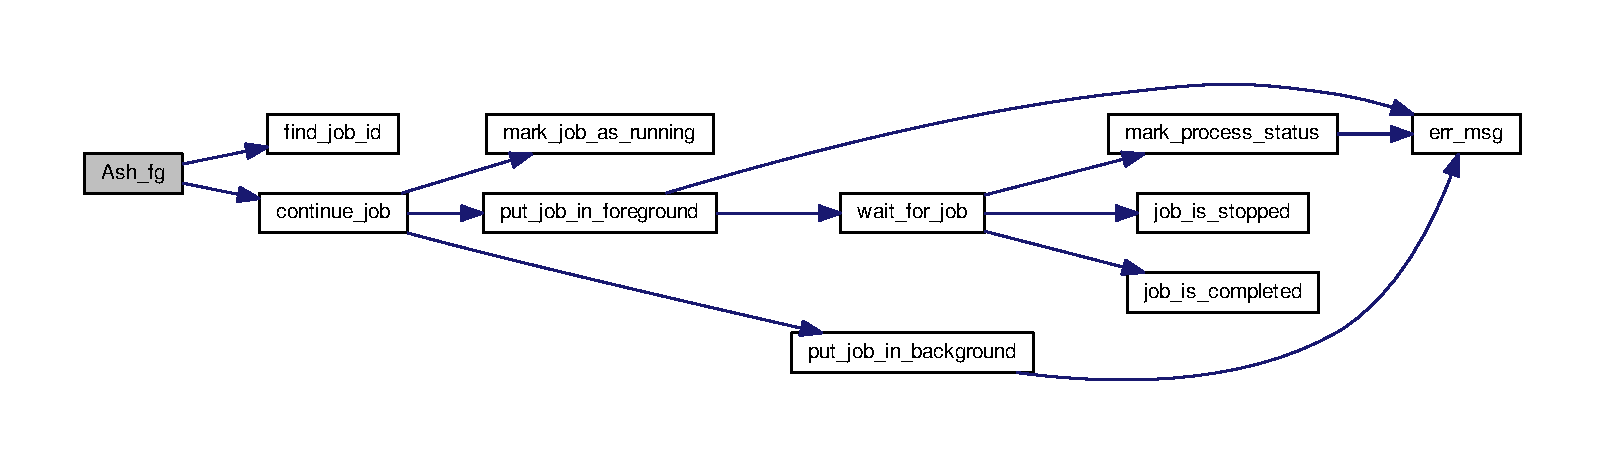
\includegraphics[width=350pt]{job_8c_a792fcc9814d020b087911591c5fce10b_cgraph}
\end{center}
\end{figure}


\hypertarget{job_8c_a4242d3cdbc0468d774243dc67b330296}{\index{job.\-c@{job.\-c}!Ash\-\_\-help@{Ash\-\_\-help}}
\index{Ash\-\_\-help@{Ash\-\_\-help}!job.c@{job.\-c}}
\subsubsection[{Ash\-\_\-help}]{\setlength{\rightskip}{0pt plus 5cm}int Ash\-\_\-help (
\begin{DoxyParamCaption}
\item[{{\bf Process} $\ast$}]{p, }
\item[{int}]{in\-\_\-file, }
\item[{int}]{out\-\_\-file, }
\item[{int}]{err\-\_\-file}
\end{DoxyParamCaption}
)}}\label{job_8c_a4242d3cdbc0468d774243dc67b330296}


\mbox{[}B\-U\-I\-L\-T\-I\-N\mbox{]}\-: Prints a help message for the shell. 

\begin{DoxyParagraph}{Description}
This shell builtin is used print a help message for the shell. It accepts the following grammar \-: \par
help \par
 
\end{DoxyParagraph}

\begin{DoxyParams}{Parameters}
{\em p} & This is a process (\hyperlink{struct__process}{\-\_\-process}) . It is not of interest to this builtin.\\
\hline
{\em in\-\_\-file} & File descriptor to the builtin's standard input.\\
\hline
{\em out\-\_\-file} & File descriptor to the builtin's standard output.\\
\hline
{\em in\-\_\-file} & File descriptor to the builtin's standard error.\\
\hline
\end{DoxyParams}
\begin{DoxyReturn}{Returns}
Always returns {\itshape 0}.
\end{DoxyReturn}
\begin{DoxySeeAlso}{See Also}
\hyperlink{struct__process}{\-\_\-process}, {\itshape dprintf()}, \hyperlink{job_8h_a2c2cfa6591ee05cc5bf0c39f38b9e2ea}{Ash\-\_\-cd()}, \hyperlink{job_8h_a9fa5abe15df71a688905dc7b29a1389f}{Ash\-\_\-exit()}, \hyperlink{job_8h_a8950ee4bf84f8322e0b294d0c448a9e7}{Ash\-\_\-jobs()}, \hyperlink{job_8h_a9bc6f26d0ab14359707a0f367f1a6522}{Ash\-\_\-bg()}, \hyperlink{job_8h_a723e6648fca47a139cdff5cf4f1bc4bb}{Ash\-\_\-kill()}, and \hyperlink{job_8h_a07e5c62e1d5e55012cf188dd32b6cf27}{Ash\-\_\-killall()} 
\end{DoxySeeAlso}
\hypertarget{job_8c_a8950ee4bf84f8322e0b294d0c448a9e7}{\index{job.\-c@{job.\-c}!Ash\-\_\-jobs@{Ash\-\_\-jobs}}
\index{Ash\-\_\-jobs@{Ash\-\_\-jobs}!job.c@{job.\-c}}
\subsubsection[{Ash\-\_\-jobs}]{\setlength{\rightskip}{0pt plus 5cm}int Ash\-\_\-jobs (
\begin{DoxyParamCaption}
\item[{{\bf Process} $\ast$}]{p, }
\item[{int}]{in\-\_\-file, }
\item[{int}]{out\-\_\-file, }
\item[{int}]{err\-\_\-file}
\end{DoxyParamCaption}
)}}\label{job_8c_a8950ee4bf84f8322e0b294d0c448a9e7}


\mbox{[}B\-U\-I\-L\-T\-I\-N\mbox{]}\-: List the jobs in the shell's active job list. 

\begin{DoxyParagraph}{Description}
This shell builtin is used list the jobs (\hyperlink{struct__job}{\-\_\-job}) in the shell's active job list (\hyperlink{job_8c_a4ca397eaae80b0004f61dad81729c06d}{job\-\_\-list\-\_\-head}). It accepts the following grammar \-: \par
jobs \par
To list the jobs, it does the following \-: \begin{DoxyItemize}
\item Calls update() status to update the status of child processes (\hyperlink{struct__process}{\-\_\-process}) of the shell. \item Traverses the active job list, and for each job on the list, it prints its status and then calls \hyperlink{job_8h_ae54ca57ee056e74d8ae32967453e4482}{print\-\_\-job\-\_\-command()} to print the command that started the job. An active job can be in one of three states\-: (1) {\itshape Running} , (2) {\itshape Stopped} , or (3) {\itshape Done} . The function calls \hyperlink{job_8h_a0654ba7330ec47c1e636afe60657651b}{job\-\_\-is\-\_\-completed()}, and \hyperlink{job_8h_a4b49892bffa5095eb5a0fb7d86659456}{job\-\_\-is\-\_\-stopped()} to determine if an active job is either completed, or stopped, respectively.\end{DoxyItemize}

\end{DoxyParagraph}

\begin{DoxyParams}{Parameters}
{\em p} & This is a process (\hyperlink{struct__process}{\-\_\-process}) . It is not of interest to this builtin.\\
\hline
{\em in\-\_\-file} & File descriptor to the builtin's standard input.\\
\hline
{\em out\-\_\-file} & File descriptor to the builtin's standard output.\\
\hline
{\em in\-\_\-file} & File descriptor to the builtin's standard error.\\
\hline
\end{DoxyParams}
\begin{DoxyReturn}{Returns}
Returns {\itshape 0} .
\end{DoxyReturn}
\begin{DoxySeeAlso}{See Also}
\hyperlink{struct__process}{\-\_\-process}, \hyperlink{job_8h_ad8e58b77db46018eeb20c68855538f35}{update\-\_\-status()}, \hyperlink{struct__job}{\-\_\-job}, \hyperlink{job_8c_a4ca397eaae80b0004f61dad81729c06d}{job\-\_\-list\-\_\-head}, \hyperlink{job_8h_a0654ba7330ec47c1e636afe60657651b}{job\-\_\-is\-\_\-completed()}, \hyperlink{job_8h_a4b49892bffa5095eb5a0fb7d86659456}{job\-\_\-is\-\_\-stopped()}, {\itshape dprintf()}, \hyperlink{job_8h_ae54ca57ee056e74d8ae32967453e4482}{print\-\_\-job\-\_\-command()}, \hyperlink{job_8h_abd1ac77dca84a11371146d61dbe2c35d}{\-\_\-job\-\_\-state}, \hyperlink{job_8c_a1a6160b9abc239f381d9ba30d00b4e0d}{job\-\_\-states}, \hyperlink{job_8h_a2c2cfa6591ee05cc5bf0c39f38b9e2ea}{Ash\-\_\-cd()}, \hyperlink{job_8h_a9fa5abe15df71a688905dc7b29a1389f}{Ash\-\_\-exit()}, \hyperlink{job_8h_a792fcc9814d020b087911591c5fce10b}{Ash\-\_\-fg()}, \hyperlink{job_8h_a9bc6f26d0ab14359707a0f367f1a6522}{Ash\-\_\-bg()}, \hyperlink{job_8h_a4242d3cdbc0468d774243dc67b330296}{Ash\-\_\-help()}, \hyperlink{job_8h_a723e6648fca47a139cdff5cf4f1bc4bb}{Ash\-\_\-kill()}, and \hyperlink{job_8h_a07e5c62e1d5e55012cf188dd32b6cf27}{Ash\-\_\-killall()} 
\end{DoxySeeAlso}


Here is the call graph for this function\-:\nopagebreak
\begin{figure}[H]
\begin{center}
\leavevmode
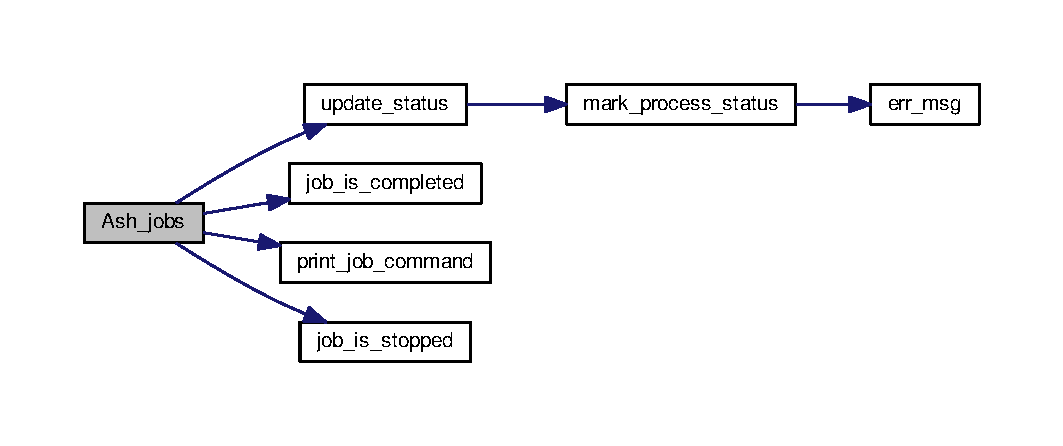
\includegraphics[width=350pt]{job_8c_a8950ee4bf84f8322e0b294d0c448a9e7_cgraph}
\end{center}
\end{figure}


\hypertarget{job_8c_a723e6648fca47a139cdff5cf4f1bc4bb}{\index{job.\-c@{job.\-c}!Ash\-\_\-kill@{Ash\-\_\-kill}}
\index{Ash\-\_\-kill@{Ash\-\_\-kill}!job.c@{job.\-c}}
\subsubsection[{Ash\-\_\-kill}]{\setlength{\rightskip}{0pt plus 5cm}int Ash\-\_\-kill (
\begin{DoxyParamCaption}
\item[{{\bf Process} $\ast$}]{p, }
\item[{int}]{in\-\_\-file, }
\item[{int}]{out\-\_\-file, }
\item[{int}]{err\-\_\-file}
\end{DoxyParamCaption}
)}}\label{job_8c_a723e6648fca47a139cdff5cf4f1bc4bb}


\mbox{[}B\-U\-I\-L\-T\-I\-N\mbox{]}\-: Sends a signal to active jobs. 

\begin{DoxyParagraph}{Description}
This shell builtin is used to send a signal to active jobs. It accepts the following grammar \-: \par
kill l $\vert$ s$<$signal-\/name$>$ $\vert$ n$<$signal-\/number$>$ -\/$<$job-\/id$>$ ... \par
The signal to be sent can be specief by using either the {\itshape s} option, or the \par
 option. The  option is used to specified a signal using its symbolic name. The symbolic name must be a case-\/insensitive string of one of the following patterns\-: \par
\begin{DoxyItemize}
\item S\-I\-Gxxx or S\-I\-Gxxxx (e.\-g., S\-I\-G\-H\-U\-P or S\-I\-G\-K\-I\-L\-L, respectively) \item xxx or xxxx (e.\-g., H\-U\-P or K\-I\-L\-L, respectively)\end{DoxyItemize}
The {\itshape n} option is used to specified the signal number to be sent (e.\-g., {\itshape n9} sends signal number 9). The {\itshape l} option is used to list the signals that can be sent. To send the signal, the function does the following \-: \begin{DoxyItemize}
\item Checks if the command grammer is valid. \item If the grammar is valid, then for each specified job, it calls \hyperlink{job_8h_a870c6d70cfb180e88d217a0b3501aedb}{find\-\_\-job\-\_\-id()} to find the job on the active job list (job\-\_\-list\-\_\-head) \item For each job that is found, it calls {\itshape kill()} to send the signal to the job.\end{DoxyItemize}

\end{DoxyParagraph}

\begin{DoxyParams}{Parameters}
{\em p} & This is a process (\hyperlink{struct__process}{\-\_\-process}) . Only its argument vector (\-\_\-process\-::argv) and argument count (\-\_\-process\-::argc) are of interest to this builtin.\\
\hline
{\em in\-\_\-file} & File descriptor to the builtin's standard input.\\
\hline
{\em out\-\_\-file} & File descriptor to the builtin's standard output.\\
\hline
{\em in\-\_\-file} & File descriptor to the builtin's standard error.\\
\hline
\end{DoxyParams}
\begin{DoxyReturn}{Returns}
Returns {\itshape 0} on success, or {\itshape -\/1} on error. Possible reasons for failure are as follows\-: \begin{DoxyItemize}
\item The grammar of the command is invalid. \item The grammar of the command is valid, but a specified {\itshape $<$job-\/id$>$} does not refer to a job on the active job list.\end{DoxyItemize}

\end{DoxyReturn}
\begin{DoxySeeAlso}{See Also}
\hyperlink{struct__process}{\-\_\-process}, \-\_\-process\-::argv, \-\_\-process\-::argc, {\itshape dprintf()}, {\itshape atoi()}, \hyperlink{struct__job}{\-\_\-job}, \hyperlink{job_8h_a870c6d70cfb180e88d217a0b3501aedb}{find\-\_\-job\-\_\-id()}, {\itshape kill()}, \-\_\-job\-::id \hyperlink{job_8h_a2c2cfa6591ee05cc5bf0c39f38b9e2ea}{Ash\-\_\-cd()}, \hyperlink{job_8h_a9fa5abe15df71a688905dc7b29a1389f}{Ash\-\_\-exit()}, \hyperlink{job_8h_a8950ee4bf84f8322e0b294d0c448a9e7}{Ash\-\_\-jobs()}, \hyperlink{job_8h_a9bc6f26d0ab14359707a0f367f1a6522}{Ash\-\_\-bg()}, \hyperlink{job_8h_a4242d3cdbc0468d774243dc67b330296}{Ash\-\_\-help()}, \hyperlink{job_8h_a723e6648fca47a139cdff5cf4f1bc4bb}{Ash\-\_\-kill()}, and \hyperlink{job_8h_a07e5c62e1d5e55012cf188dd32b6cf27}{Ash\-\_\-killall()}
\end{DoxySeeAlso}
\begin{DoxyRefDesc}{Todo}
\item[\hyperlink{todo__todo000002}{Todo}]implement more signals, build an array of signal names\end{DoxyRefDesc}


Here is the call graph for this function\-:\nopagebreak
\begin{figure}[H]
\begin{center}
\leavevmode
\includegraphics[width=232pt]{job_8c_a723e6648fca47a139cdff5cf4f1bc4bb_cgraph}
\end{center}
\end{figure}


\hypertarget{job_8c_a07e5c62e1d5e55012cf188dd32b6cf27}{\index{job.\-c@{job.\-c}!Ash\-\_\-killall@{Ash\-\_\-killall}}
\index{Ash\-\_\-killall@{Ash\-\_\-killall}!job.c@{job.\-c}}
\subsubsection[{Ash\-\_\-killall}]{\setlength{\rightskip}{0pt plus 5cm}int Ash\-\_\-killall (
\begin{DoxyParamCaption}
\item[{{\bf Process} $\ast$}]{p, }
\item[{int}]{in\-\_\-file, }
\item[{int}]{out\-\_\-file, }
\item[{int}]{err\-\_\-file}
\end{DoxyParamCaption}
)}}\label{job_8c_a07e5c62e1d5e55012cf188dd32b6cf27}


\mbox{[}B\-U\-I\-L\-T\-I\-N\mbox{]}\-: Sends a signal to all active jobs. 

\begin{DoxyParagraph}{Description}
This shell builtin is used to send a signal to all jobs on the active job list (\hyperlink{job_8c_a4ca397eaae80b0004f61dad81729c06d}{job\-\_\-list\-\_\-head}). It accepts the following grammar \-: \par
killall l or killall s$<$signal-\/name$>$ $\vert$ n$<$signal-\/number$>$ \par
The signal to be sent can be specief by using either the {\itshape s} option, or the \par
 option. The  option is used to specified a signal using its symbolic name. The symbolic name must be a case-\/insensitive string of one of the following patterns\-: \par
\begin{DoxyItemize}
\item S\-I\-Gxxx or S\-I\-Gxxxx (e.\-g., S\-I\-G\-H\-U\-P or S\-I\-G\-K\-I\-L\-L, respectively) \item xxx or xxxx (e.\-g., H\-U\-P or K\-I\-L\-L, respectively)\end{DoxyItemize}
The {\itshape n} option is used to specified the signal number to be sent (e.\-g., {\itshape n9} sends signal number 9). The {\itshape l} option is used to list the signals that can be sent. To send the signal, the function does the following \-: \begin{DoxyItemize}
\item Checks if the command grammer is valid. \item If the grammar is valid, then it calls () to send the singal to all active jobs.\end{DoxyItemize}

\end{DoxyParagraph}

\begin{DoxyParams}{Parameters}
{\em p} & This is a process (\hyperlink{struct__process}{\-\_\-process}) . Only its argument vector (\-\_\-process\-::argv) and argument count (\-\_\-process\-::argc) are of interest to this builtin.\\
\hline
{\em in\-\_\-file} & File descriptor to the builtin's standard input.\\
\hline
{\em out\-\_\-file} & File descriptor to the builtin's standard output.\\
\hline
{\em in\-\_\-file} & File descriptor to the builtin's standard error.\\
\hline
\end{DoxyParams}
\begin{DoxyReturn}{Returns}
Returns {\itshape 0} on success, or {\itshape -\/1} on error. Possible reasons for failure are as follows\-: \begin{DoxyItemize}
\item The grammar of the command is invalid.\end{DoxyItemize}

\end{DoxyReturn}
\begin{DoxySeeAlso}{See Also}
\hyperlink{struct__process}{\-\_\-process}, \-\_\-process\-::argv, \-\_\-process\-::argc, {\itshape dprintf()}, {\itshape kill()}, \hyperlink{job_8h_a2c2cfa6591ee05cc5bf0c39f38b9e2ea}{Ash\-\_\-cd()}, \hyperlink{job_8h_a9fa5abe15df71a688905dc7b29a1389f}{Ash\-\_\-exit()}, \hyperlink{job_8h_a8950ee4bf84f8322e0b294d0c448a9e7}{Ash\-\_\-jobs()}, \hyperlink{job_8h_a9bc6f26d0ab14359707a0f367f1a6522}{Ash\-\_\-bg()}, \hyperlink{job_8h_a4242d3cdbc0468d774243dc67b330296}{Ash\-\_\-help()}, and \hyperlink{job_8h_a723e6648fca47a139cdff5cf4f1bc4bb}{Ash\-\_\-kill}. 
\end{DoxySeeAlso}
\begin{DoxyRefDesc}{Todo}
\item[\hyperlink{todo__todo000003}{Todo}]implement more signals, build an array of signal names\end{DoxyRefDesc}
\hypertarget{job_8c_ab69ad21398604a048a5a1b4ef7af1320}{\index{job.\-c@{job.\-c}!continue\-\_\-job@{continue\-\_\-job}}
\index{continue\-\_\-job@{continue\-\_\-job}!job.c@{job.\-c}}
\subsubsection[{continue\-\_\-job}]{\setlength{\rightskip}{0pt plus 5cm}void continue\-\_\-job (
\begin{DoxyParamCaption}
\item[{{\bf Job} $\ast$}]{j, }
\item[{int}]{foreground}
\end{DoxyParamCaption}
)}}\label{job_8c_ab69ad21398604a048a5a1b4ef7af1320}


Continues a job. 

This function is used to continue a job either in the foreground or in the background. It does the following\-: \begin{DoxyItemize}
\item Calls \hyperlink{job_8h_a690fc87028fe2334113ee8d92f8c8f24}{mark\-\_\-job\-\_\-as\-\_\-running()} to update the job's state. \item If {\itshape foreground} is non-\/zero (i.\-e., true), it calls \hyperlink{job_8h_ab3b7803e9a87944a86267abc40fe6c39}{put\-\_\-job\-\_\-in\-\_\-foreground()} to put the job in the foreground. Otherwise, it calls \hyperlink{job_8h_a095ab07b063dbbc25fd2729125fb530a}{put\-\_\-job\-\_\-in\-\_\-background()} to put the job in the background.\end{DoxyItemize}

\begin{DoxyParams}{Parameters}
{\em j} & The job to continue.\\
\hline
{\em foreground} & Determines if the job is to be continued in the foreground or in the background. If this value is non-\/zero (i.\-e., true), then the job is continued in the foreground. Otherwise, it is continued in the background.\\
\hline
\end{DoxyParams}
\begin{DoxyReturn}{Returns}
Returns {\itshape void} .
\end{DoxyReturn}
\begin{DoxySeeAlso}{See Also}
\hyperlink{struct__job}{\-\_\-job}, \hyperlink{job_8h_a690fc87028fe2334113ee8d92f8c8f24}{mark\-\_\-job\-\_\-as\-\_\-running()}, \hyperlink{job_8h_ab3b7803e9a87944a86267abc40fe6c39}{put\-\_\-job\-\_\-in\-\_\-foreground()}, \hyperlink{job_8h_a095ab07b063dbbc25fd2729125fb530a}{put\-\_\-job\-\_\-in\-\_\-background()}, \hyperlink{job_8h_a9bc6f26d0ab14359707a0f367f1a6522}{Ash\-\_\-bg()}, \hyperlink{job_8h_abd1ac77dca84a11371146d61dbe2c35d}{\-\_\-job\-\_\-state}, \hyperlink{job_8c_a1a6160b9abc239f381d9ba30d00b4e0d}{job\-\_\-states}, and \hyperlink{job_8h_a792fcc9814d020b087911591c5fce10b}{Ash\-\_\-fg()}. 
\end{DoxySeeAlso}


Here is the call graph for this function\-:\nopagebreak
\begin{figure}[H]
\begin{center}
\leavevmode
\includegraphics[width=350pt]{job_8c_ab69ad21398604a048a5a1b4ef7af1320_cgraph}
\end{center}
\end{figure}




Here is the caller graph for this function\-:\nopagebreak
\begin{figure}[H]
\begin{center}
\leavevmode
\includegraphics[width=238pt]{job_8c_ab69ad21398604a048a5a1b4ef7af1320_icgraph}
\end{center}
\end{figure}


\hypertarget{job_8c_a18d3d13da14c1f38fa2b0932e8850129}{\index{job.\-c@{job.\-c}!create\-\_\-job@{create\-\_\-job}}
\index{create\-\_\-job@{create\-\_\-job}!job.c@{job.\-c}}
\subsubsection[{create\-\_\-job}]{\setlength{\rightskip}{0pt plus 5cm}{\bf Job}$\ast$ create\-\_\-job (
\begin{DoxyParamCaption}
\item[{void}]{}
\end{DoxyParamCaption}
)}}\label{job_8c_a18d3d13da14c1f38fa2b0932e8850129}


Creates a new job instance. 

\begin{DoxyParagraph}{Description}
This function is used to create a new job (\hyperlink{struct__job}{\-\_\-job}) instance. It does the following\-: \begin{DoxyItemize}
\item Dynamically allocate memory for a job instance. \item Assign default values to all the fields in the job instance.\end{DoxyItemize}

\end{DoxyParagraph}
\begin{DoxyReturn}{Returns}
Returns a pointer to the newly create job instance on success, or N\-U\-L\-L on failure.
\end{DoxyReturn}
\begin{DoxySeeAlso}{See Also}
\hyperlink{struct__job}{\-\_\-job}, \#\-M\-A\-X\-\_\-\-P\-R\-O\-C\-E\-S\-S\-E\-S, and {\itshape malloc()}. 
\end{DoxySeeAlso}


Here is the call graph for this function\-:\nopagebreak
\begin{figure}[H]
\begin{center}
\leavevmode
\includegraphics[width=230pt]{job_8c_a18d3d13da14c1f38fa2b0932e8850129_cgraph}
\end{center}
\end{figure}


\hypertarget{job_8c_a1af7ca10dbe6b9358262cc18f04bf6f5}{\index{job.\-c@{job.\-c}!create\-\_\-process@{create\-\_\-process}}
\index{create\-\_\-process@{create\-\_\-process}!job.c@{job.\-c}}
\subsubsection[{create\-\_\-process}]{\setlength{\rightskip}{0pt plus 5cm}{\bf Process}$\ast$ create\-\_\-process (
\begin{DoxyParamCaption}
\item[{void}]{}
\end{DoxyParamCaption}
)}}\label{job_8c_a1af7ca10dbe6b9358262cc18f04bf6f5}


Creates an instance of a process. 

\begin{DoxyParagraph}{Description}
This function is used to create an instance of a process (\hyperlink{struct__process}{\-\_\-process}). It does the following \-: \begin{DoxyItemize}
\item Dynamically allocate memory for an instance of a process. \item Assigns default values to all fields of the process instance.\end{DoxyItemize}

\end{DoxyParagraph}
\begin{DoxyReturn}{Returns}
Returns N\-U\-L\-L on failure, or a pointer to the allocated memory on success.
\end{DoxyReturn}
@ sa \hyperlink{struct__process}{\-\_\-process}, Process, \#\-Max\-\_\-\-A\-R\-G\-S, and \hyperlink{job_8h_a9c2d0895268bd3229fc231b00029eb7b}{process\-\_\-dup()}. 

Here is the call graph for this function\-:\nopagebreak
\begin{figure}[H]
\begin{center}
\leavevmode
\includegraphics[width=252pt]{job_8c_a1af7ca10dbe6b9358262cc18f04bf6f5_cgraph}
\end{center}
\end{figure}




Here is the caller graph for this function\-:\nopagebreak
\begin{figure}[H]
\begin{center}
\leavevmode
\includegraphics[width=350pt]{job_8c_a1af7ca10dbe6b9358262cc18f04bf6f5_icgraph}
\end{center}
\end{figure}


\hypertarget{job_8c_a8c729ad459ad99d7a0e3c7a549d98383}{\index{job.\-c@{job.\-c}!destroy\-\_\-job@{destroy\-\_\-job}}
\index{destroy\-\_\-job@{destroy\-\_\-job}!job.c@{job.\-c}}
\subsubsection[{destroy\-\_\-job}]{\setlength{\rightskip}{0pt plus 5cm}int destroy\-\_\-job (
\begin{DoxyParamCaption}
\item[{{\bf Job} $\ast$}]{j}
\end{DoxyParamCaption}
)}}\label{job_8c_a8c729ad459ad99d7a0e3c7a549d98383}


Destroys a job. 

\begin{DoxyParagraph}{Description}
This function is used to destroy a job (\hyperlink{struct__job}{\-\_\-job}). It does the following\-: \begin{DoxyItemize}
\item Calls \hyperlink{job_8h_a167097d11d4b3ceda7957cb5244de3a8}{destroy\-\_\-process()} to destroy all of the process (\-\_\-job\-::num\-\_\-processes) currently stored in the job's process list (\-\_\-job\-::processes). \item Calls \hyperlink{err_8h_a40bd4201ea3cf1b6f8e7fef01362bf67}{sfree()} to free the pathnames of the job's I/\-O redirection files (\-\_\-job\-::in\-\_\-file, \-\_\-job\-::out\-\_\-file, and \-\_\-job\-::err\-\_\-file). \item Calls \hyperlink{err_8h_a40bd4201ea3cf1b6f8e7fef01362bf67}{sfree()} to free the job instance itself.\end{DoxyItemize}

\end{DoxyParagraph}

\begin{DoxyParams}{Parameters}
{\em j} & The job to destroy.\\
\hline
\end{DoxyParams}
\begin{DoxyReturn}{Returns}
Returns {\itshape -\/1} on failure, or {\itshape 0} on success.
\end{DoxyReturn}
\begin{DoxySeeAlso}{See Also}
\hyperlink{struct__job}{\-\_\-job}, \-\_\-job\-::num\-\_\-processes, \hyperlink{job_8h_a167097d11d4b3ceda7957cb5244de3a8}{destroy\-\_\-process()}, \-\_\-job\-::processes, \-\_\-job\-::in\-\_\-file, \-\_\-job\-::out\-\_\-file, and \-\_\-job\-::err\-\_\-file. 
\end{DoxySeeAlso}


Here is the call graph for this function\-:\nopagebreak
\begin{figure}[H]
\begin{center}
\leavevmode
\includegraphics[width=274pt]{job_8c_a8c729ad459ad99d7a0e3c7a549d98383_cgraph}
\end{center}
\end{figure}




Here is the caller graph for this function\-:\nopagebreak
\begin{figure}[H]
\begin{center}
\leavevmode
\includegraphics[width=282pt]{job_8c_a8c729ad459ad99d7a0e3c7a549d98383_icgraph}
\end{center}
\end{figure}


\hypertarget{job_8c_a167097d11d4b3ceda7957cb5244de3a8}{\index{job.\-c@{job.\-c}!destroy\-\_\-process@{destroy\-\_\-process}}
\index{destroy\-\_\-process@{destroy\-\_\-process}!job.c@{job.\-c}}
\subsubsection[{destroy\-\_\-process}]{\setlength{\rightskip}{0pt plus 5cm}void destroy\-\_\-process (
\begin{DoxyParamCaption}
\item[{{\bf Process} $\ast$}]{p}
\end{DoxyParamCaption}
)}}\label{job_8c_a167097d11d4b3ceda7957cb5244de3a8}


Destroys a process instance. 

\begin{DoxyParagraph}{Description}
This function is used to destroy a process (\hyperlink{struct__process}{\-\_\-process}) instance. It does the following \-: \begin{DoxyItemize}
\item Calls \hyperlink{err_8h_a40bd4201ea3cf1b6f8e7fef01362bf67}{sfree()} to free the arguments (\-\_\-process\-::argc) currently stored in the argument vector (\hyperlink{struct__process}{\-\_\-process}\-:argv) of the process. \item Calls \hyperlink{err_8h_a40bd4201ea3cf1b6f8e7fef01362bf67}{sfree()} to free the process instance itself.\end{DoxyItemize}

\end{DoxyParagraph}
\begin{DoxyReturn}{Returns}
Returns {\itshape void} .
\end{DoxyReturn}
\begin{DoxySeeAlso}{See Also}
\hyperlink{struct__process}{\-\_\-process}, \-\_\-process\-::argv, \-\_\-process\-::argc, \hyperlink{err_8h_a40bd4201ea3cf1b6f8e7fef01362bf67}{sfree()}, and \hyperlink{job_8h_a8c729ad459ad99d7a0e3c7a549d98383}{destroy\-\_\-job()}. 
\end{DoxySeeAlso}


Here is the caller graph for this function\-:\nopagebreak
\begin{figure}[H]
\begin{center}
\leavevmode
\includegraphics[width=350pt]{job_8c_a167097d11d4b3ceda7957cb5244de3a8_icgraph}
\end{center}
\end{figure}


\hypertarget{job_8c_a75430387f345a954b011547bf14a56ce}{\index{job.\-c@{job.\-c}!do\-\_\-job\-\_\-notification@{do\-\_\-job\-\_\-notification}}
\index{do\-\_\-job\-\_\-notification@{do\-\_\-job\-\_\-notification}!job.c@{job.\-c}}
\subsubsection[{do\-\_\-job\-\_\-notification}]{\setlength{\rightskip}{0pt plus 5cm}void do\-\_\-job\-\_\-notification (
\begin{DoxyParamCaption}
\item[{void}]{}
\end{DoxyParamCaption}
)}}\label{job_8c_a75430387f345a954b011547bf14a56ce}


Notifies the user of job status updates. 

\begin{DoxyParagraph}{Description}
This function is used to notify the user of job (\hyperlink{struct__job}{\-\_\-job}) status updates. It does the following\-: \begin{DoxyItemize}
\item Calls \hyperlink{job_8h_ad8e58b77db46018eeb20c68855538f35}{update\-\_\-status()} to update the status of stopped or completed processes (\hyperlink{struct__process}{\-\_\-process}). \item For each job in the active job list (\hyperlink{job_8c_a4ca397eaae80b0004f61dad81729c06d}{job\-\_\-list\-\_\-head}), it checks if the job has either completed (by calling \hyperlink{job_8h_a4b49892bffa5095eb5a0fb7d86659456}{job\-\_\-is\-\_\-stopped()} or stopped ( by calling \hyperlink{job_8h_a0654ba7330ec47c1e636afe60657651b}{job\-\_\-is\-\_\-completed()}). If a job is completed and is not a foreground job, it notifies the user (by calling \hyperlink{job_8h_ae7a22fe41ac695db73564a23ce25cf6a}{format\-\_\-job\-\_\-info()}), and then removes the job from the active job list by calling \hyperlink{job_8h_a8c729ad459ad99d7a0e3c7a549d98383}{destroy\-\_\-job()}. If a job is stopped, and its changed status has not yet been reported, the function reports its status by calling format\-\_\-job\-\_\-status(), and then set its \-\_\-job\-::notified field to {\itshape 1}.\end{DoxyItemize}

\end{DoxyParagraph}
\begin{DoxyReturn}{Returns}
Returns void.
\end{DoxyReturn}
\begin{DoxySeeAlso}{See Also}
\hyperlink{job_8h_ad8e58b77db46018eeb20c68855538f35}{update\-\_\-status()}, \hyperlink{job_8c_a4ca397eaae80b0004f61dad81729c06d}{job\-\_\-list\-\_\-head}, \hyperlink{job_8h_a0654ba7330ec47c1e636afe60657651b}{job\-\_\-is\-\_\-completed()}, \hyperlink{job_8h_a4b49892bffa5095eb5a0fb7d86659456}{job\-\_\-is\-\_\-stopped()}, \hyperlink{job_8h_ae7a22fe41ac695db73564a23ce25cf6a}{format\-\_\-job\-\_\-info()}, and \-\_\-job\-::notified. 
\end{DoxySeeAlso}


Here is the call graph for this function\-:\nopagebreak
\begin{figure}[H]
\begin{center}
\leavevmode
\includegraphics[width=350pt]{job_8c_a75430387f345a954b011547bf14a56ce_cgraph}
\end{center}
\end{figure}


\hypertarget{job_8c_a328634c49391a29ef1d4e86d6bf0ea7e}{\index{job.\-c@{job.\-c}!execute\-\_\-job@{execute\-\_\-job}}
\index{execute\-\_\-job@{execute\-\_\-job}!job.c@{job.\-c}}
\subsubsection[{execute\-\_\-job}]{\setlength{\rightskip}{0pt plus 5cm}int execute\-\_\-job (
\begin{DoxyParamCaption}
\item[{{\bf Job} $\ast$}]{j}
\end{DoxyParamCaption}
)}}\label{job_8c_a328634c49391a29ef1d4e86d6bf0ea7e}

\begin{DoxyParams}{Parameters}
{\em Executes} & a job.\\
\hline
\end{DoxyParams}
\begin{DoxyParagraph}{Description}
This function is used to execute a job (\hyperlink{struct__job}{\-\_\-job}). It does the following \-: \begin{DoxyItemize}
\item Performs I/\-O redirections for the job, if nessasary. \item Sets up pipes, if nessasary. \item For each process (\hyperlink{struct__process}{\-\_\-process}) in the job, the function checks if it refers to a shell builtin via \hyperlink{job_8h_a028aee0dd87474ee61f6c654efe653a2}{is\-\_\-builtin()}. If the process refers to a builtin, the builtin is launched. Otherwise, the function forks a child, and the child then calls \hyperlink{job_8h_acaa6f75b768f52660498b9fab3898e15}{execute\-\_\-process()} to {\itshape exec} a new program. \item Cleans up after pipes. \item After all processes in the job have been launched or executed, the function adds the job to the active job list via \hyperlink{job_8h_aff64d308dd49d9da9f2d6f993346f7ad}{add\-\_\-job\-\_\-to\-\_\-list()}. In additiion, if \hyperlink{job_8c_af7730a56d05055a70f3c18ee938209f8}{Ash\-\_\-is\-\_\-interactive} is non-\/zero, it calls \hyperlink{job_8h_aead235b523c076d6346ba285fa98f6d1}{wait\-\_\-for\-\_\-job()} to wait for the job. If \hyperlink{job_8c_af7730a56d05055a70f3c18ee938209f8}{Ash\-\_\-is\-\_\-interactive} is {\itshape 0} and the job's foreground field (\-\_\-job\-::foreground) is non-\/zero, the function calls \hyperlink{job_8h_ab3b7803e9a87944a86267abc40fe6c39}{put\-\_\-job\-\_\-in\-\_\-foreground()} to put the job in the foreground. Otherwise, it calls \hyperlink{job_8h_a095ab07b063dbbc25fd2729125fb530a}{put\-\_\-job\-\_\-in\-\_\-background()} to put the job in the background.\end{DoxyItemize}

\end{DoxyParagraph}

\begin{DoxyParams}{Parameters}
{\em j} & The job to execute.\\
\hline
\end{DoxyParams}
\begin{DoxyReturn}{Returns}
Returns {\itshape 0} on success, or {\itshape -\/1} on failure. Possible reasons for failure are as follows\-: \begin{DoxyItemize}
\item Performing I/\-O redirection for the job failed. \item Setting up pipes failed. \item A shell builtin failed. \item Forking a child failed. \item Cleaning up after pipes (i.\-e., closing file descriptors) failed.\end{DoxyItemize}
when any of the events above occurs, the function returns immidiately, and the job is never added to the active job list.
\end{DoxyReturn}
\begin{DoxySeeAlso}{See Also}
{\itshape job, \hyperlink{struct__process}{\-\_\-process}, \-\_\-job\-::in\-\_\-file, \-\_\-job\-::out\-\_\-file, \-\_\-job\-::err\-\_\-file, \-\_\-job\-::stdin}, {\itshape job\-::stdout}, {\itshape job\-::stderr}, {\itshape open()}, \-\_\-job\-::num\-\_\-processes, \-\_\-job\-::processes, {\itshape pipe()}, \hyperlink{job_8h_a028aee0dd87474ee61f6c654efe653a2}{is\-\_\-builtin()}, \hyperlink{job_8c_a2c5551422426f406568d84844b40acb9}{builtins}, {\itshape fork()}, \hyperlink{job_8h_acaa6f75b768f52660498b9fab3898e15}{execute\-\_\-process()}, \hyperlink{err_8c_a07dfb9fd24fe41a9f703bd92af2cf646}{err\-\_\-msg()}, \hyperlink{job_8c_af7730a56d05055a70f3c18ee938209f8}{Ash\-\_\-is\-\_\-interactive}, {\itshape setpgid()}, {\itshape close()}, \hyperlink{job_8h_aff64d308dd49d9da9f2d6f993346f7ad}{add\-\_\-job\-\_\-to\-\_\-list()}, \hyperlink{job_8h_aead235b523c076d6346ba285fa98f6d1}{wait\-\_\-for\-\_\-job()}, \-\_\-job\-::foreground, \hyperlink{job_8h_ab3b7803e9a87944a86267abc40fe6c39}{put\-\_\-job\-\_\-in\-\_\-foreground()}, \hyperlink{job_8h_a095ab07b063dbbc25fd2729125fb530a}{put\-\_\-job\-\_\-in\-\_\-background()}, and \hyperlink{job_8h_ae7a22fe41ac695db73564a23ce25cf6a}{format\-\_\-job\-\_\-info()}.
\end{DoxySeeAlso}
\begin{DoxyRefDesc}{Todo}
\item[\hyperlink{todo__todo000001}{Todo}]Find a way for a forked child to inform the function if it calling {\itshape exec()} fails.\end{DoxyRefDesc}


Here is the call graph for this function\-:\nopagebreak
\begin{figure}[H]
\begin{center}
\leavevmode
\includegraphics[width=350pt]{job_8c_a328634c49391a29ef1d4e86d6bf0ea7e_cgraph}
\end{center}
\end{figure}


\hypertarget{job_8c_acaa6f75b768f52660498b9fab3898e15}{\index{job.\-c@{job.\-c}!execute\-\_\-process@{execute\-\_\-process}}
\index{execute\-\_\-process@{execute\-\_\-process}!job.c@{job.\-c}}
\subsubsection[{execute\-\_\-process}]{\setlength{\rightskip}{0pt plus 5cm}void execute\-\_\-process (
\begin{DoxyParamCaption}
\item[{{\bf Process} $\ast$}]{p, }
\item[{pid\-\_\-t}]{pgid, }
\item[{int}]{in\-\_\-file, }
\item[{int}]{out\-\_\-file, }
\item[{int}]{err\-\_\-file, }
\item[{int}]{foreground}
\end{DoxyParamCaption}
)}}\label{job_8c_acaa6f75b768f52660498b9fab3898e15}


Executes a process. 

\begin{DoxyParagraph}{Description }
This function is used to execute a process (\hyperlink{struct__process}{\-\_\-process}). It does the following\-: \begin{DoxyItemize}
\item If the shell is running interactively (i.\-e. \hyperlink{job_8c_af7730a56d05055a70f3c18ee938209f8}{Ash\-\_\-is\-\_\-interactive} is non-\/zero), then this function puts the process in the same process group of the job (\hyperlink{struct__job}{\-\_\-job}, \-\_\-job\-::pgid) to which it belongs. If the process is the first in the job, then it becomes the group leader of the job. \item If the shell is running interactively, and {\itshape foreground} is non-\/zero, then this function makes the group to which the process belong the foreground process group for the session and the controlling terminal (\hyperlink{job_8c_a079811c5e88059665d23821b4a38802a}{Ash\-\_\-terminal}). \item When the shell initializes itself via \hyperlink{job_8h_a3a5b33cdd8fb591704c9adfcf908a273}{init\-\_\-shell()} , it sets the disposition of all job control stop signals to S\-I\-G\-\_\-\-I\-G\-N (i.\-e., it ignores those signals). Consequently, each child it creates inherits those signal dispostions. If the shell is running interactively, then this function resets the disposition of those signals to S\-I\-G\-\_\-\-D\-F\-L (i.\-e. default) . \item Performs I\-O redirection, if nessasary. \item execs the process.\end{DoxyItemize}

\end{DoxyParagraph}

\begin{DoxyParams}{Parameters}
{\em p} & The process to be executed.\\
\hline
{\em pgid} & If this parameter is {\itshape 0} , then this process becomes the group leader of the job to which it belongs. This happens when the process is the first one in the job.\\
\hline
{\em in\-\_\-file} & The file descriptor of the file to which standard input for this process should point. If it is not equal to S\-T\-D\-I\-N\-\_\-\-F\-I\-L\-E\-N\-O, then standard input for this process is redirected to the file reffered to by this file descriptor.\\
\hline
{\em out\-\_\-file} & The file descriptor of the file to which standard output for this process should point. If it is not equal to S\-T\-D\-O\-U\-T\-\_\-\-F\-I\-L\-E\-N\-O, then standard output for this process is redirected to the file reffered to by this file descriptor.\\
\hline
{\em err\-\_\-file} & The file descriptor of the file to which standard error for this process should point. If it is not equal to S\-T\-D\-\_\-\-F\-I\-L\-E\-N\-O, then standard error for this process is redirected to the file reffered to by this file descriptor.\\
\hline
\end{DoxyParams}
\begin{DoxyReturn}{Returns}
This function is prototyped to return {\itshape void} , but never returns . If execution of the process (i.\-e., calling {\itshape exec()}) fails, then the process terminates with \hyperlink{err_8c_ab24204e73fd5cdd4d62dc30f4794da23}{err\-\_\-exit()}.
\end{DoxyReturn}
\begin{DoxySeeAlso}{See Also}
{\itshape process, \hyperlink{struct__job}{\-\_\-job}, \-::\-\_\-job\-::foreground, \hyperlink{job_8c_af7730a56d05055a70f3c18ee938209f8}{Ash\-\_\-is\-\_\-interactive}, \hyperlink{job_8c_a079811c5e88059665d23821b4a38802a}{Ash\-\_\-terminal}, \-\_\-job\-::in\-\_\-file, \-\_\-job\-::out\-\_\-file, \-\_\-job\-::err\-\_\-file, \-\_\-job\-::stdin}, {\itshape job\-::stdout}, {\itshape job\-::stderr}, getpid(), setpgid(), tcsetpgrp(), signal(), S\-T\-D\-I\-N\-\_\-\-F\-I\-L\-E\-N\-O, S\-T\-D\-O\-U\-T\-\_\-\-F\-I\-L\-E\-N\-O, S\-T\-D\-E\-R\-R\-\_\-\-F\-I\-L\-E\-N\-O, dup2(), execvp(), \hyperlink{err_8c_ab24204e73fd5cdd4d62dc30f4794da23}{err\-\_\-exit()}, and \hyperlink{job_8h_a328634c49391a29ef1d4e86d6bf0ea7e}{execute\-\_\-job()}. 
\end{DoxySeeAlso}


Here is the call graph for this function\-:\nopagebreak
\begin{figure}[H]
\begin{center}
\leavevmode
\includegraphics[width=350pt]{job_8c_acaa6f75b768f52660498b9fab3898e15_cgraph}
\end{center}
\end{figure}




Here is the caller graph for this function\-:\nopagebreak
\begin{figure}[H]
\begin{center}
\leavevmode
\includegraphics[width=278pt]{job_8c_acaa6f75b768f52660498b9fab3898e15_icgraph}
\end{center}
\end{figure}


\hypertarget{job_8c_abbd710ae6b1b777643ee31ccac51c985}{\index{job.\-c@{job.\-c}!find\-\_\-job@{find\-\_\-job}}
\index{find\-\_\-job@{find\-\_\-job}!job.c@{job.\-c}}
\subsubsection[{find\-\_\-job}]{\setlength{\rightskip}{0pt plus 5cm}{\bf Job}$\ast$ find\-\_\-job (
\begin{DoxyParamCaption}
\item[{pid\-\_\-t}]{pgid}
\end{DoxyParamCaption}
)}}\label{job_8c_abbd710ae6b1b777643ee31ccac51c985}


Finds a job with a particular P\-G\-I\-D. 

\begin{DoxyParagraph}{Description}
This function is used to find a job (\hyperlink{struct__job}{\-\_\-job}) with a particular process group I\-D (\-\_\-job\-::pgid). It does the following\-: \begin{DoxyItemize}
\item Traverses the active job list (\hyperlink{job_8c_a4ca397eaae80b0004f61dad81729c06d}{job\-\_\-list\-\_\-head}) and checks if there is a job on the list whose process group I\-D is {\itshape pgid} . If a job is found, the function returns a pointer to it.\end{DoxyItemize}

\end{DoxyParagraph}

\begin{DoxyParams}{Parameters}
{\em pgid} & The process group I\-D of the job to find.\\
\hline
\end{DoxyParams}
\begin{DoxyReturn}{Returns}
Returns a pointer to a job on success (i.\-e., a job is found), or N\-U\-L\-L on failure (i.\-e., no job with process group I\-D {\itshape pgid} was found on the job list).
\end{DoxyReturn}
\begin{DoxySeeAlso}{See Also}
\hyperlink{struct__job}{\-\_\-job}, \hyperlink{job_8c_a4ca397eaae80b0004f61dad81729c06d}{job\-\_\-list\-\_\-head}, and \-\_\-job\-::pgid. 
\end{DoxySeeAlso}
\hypertarget{job_8c_a870c6d70cfb180e88d217a0b3501aedb}{\index{job.\-c@{job.\-c}!find\-\_\-job\-\_\-id@{find\-\_\-job\-\_\-id}}
\index{find\-\_\-job\-\_\-id@{find\-\_\-job\-\_\-id}!job.c@{job.\-c}}
\subsubsection[{find\-\_\-job\-\_\-id}]{\setlength{\rightskip}{0pt plus 5cm}{\bf Job}$\ast$ find\-\_\-job\-\_\-id (
\begin{DoxyParamCaption}
\item[{int}]{id}
\end{DoxyParamCaption}
)}}\label{job_8c_a870c6d70cfb180e88d217a0b3501aedb}


Finds a job with a particular I\-D. 

\begin{DoxyParagraph}{Description}
This function is used to find a job (\hyperlink{struct__job}{\-\_\-job}) with a particular job I\-D (\-\_\-job\-::id). It does the following\-: \begin{DoxyItemize}
\item Traverses the active job list (\hyperlink{job_8c_a4ca397eaae80b0004f61dad81729c06d}{job\-\_\-list\-\_\-head}) and checks if there is a job on the list whose I\-D is {\itshape id} . If a job is found, the function returns a pointer to it.\end{DoxyItemize}

\end{DoxyParagraph}

\begin{DoxyParams}{Parameters}
{\em id} & The I\-D of the job to find.\\
\hline
\end{DoxyParams}
\begin{DoxyReturn}{Returns}
Returns a pointer to a job on success (i.\-e., a job is found), or N\-U\-L\-L on failure (i.\-e., no job with I\-D {\itshape id} was found on the job list).
\end{DoxyReturn}
\begin{DoxySeeAlso}{See Also}
\hyperlink{struct__job}{\-\_\-job}, \-\_\-job\-::id, \hyperlink{job_8c_a4ca397eaae80b0004f61dad81729c06d}{job\-\_\-list\-\_\-head}, \hyperlink{job_8h_a792fcc9814d020b087911591c5fce10b}{Ash\-\_\-fg()}, \hyperlink{job_8h_a723e6648fca47a139cdff5cf4f1bc4bb}{Ash\-\_\-kill()}, and \hyperlink{job_8h_a9bc6f26d0ab14359707a0f367f1a6522}{Ash\-\_\-bg()}. 
\end{DoxySeeAlso}


Here is the caller graph for this function\-:\nopagebreak
\begin{figure}[H]
\begin{center}
\leavevmode
\includegraphics[width=232pt]{job_8c_a870c6d70cfb180e88d217a0b3501aedb_icgraph}
\end{center}
\end{figure}


\hypertarget{job_8c_ae7a22fe41ac695db73564a23ce25cf6a}{\index{job.\-c@{job.\-c}!format\-\_\-job\-\_\-info@{format\-\_\-job\-\_\-info}}
\index{format\-\_\-job\-\_\-info@{format\-\_\-job\-\_\-info}!job.c@{job.\-c}}
\subsubsection[{format\-\_\-job\-\_\-info}]{\setlength{\rightskip}{0pt plus 5cm}void format\-\_\-job\-\_\-info (
\begin{DoxyParamCaption}
\item[{{\bf Job} $\ast$}]{j, }
\item[{const char $\ast$}]{status}
\end{DoxyParamCaption}
)}}\label{job_8c_ae7a22fe41ac695db73564a23ce25cf6a}


Formats and prints info for a job. 

\begin{DoxyParagraph}{Description}
This function is used to format and print information for a job (\hyperlink{struct__job}{\-\_\-job}). It does the following \-: \begin{DoxyItemize}
\item Formats the information. \item Prints the information to standard output.\end{DoxyItemize}

\end{DoxyParagraph}

\begin{DoxyParams}{Parameters}
{\em j} & The job whose information is to be printed.\\
\hline
{\em status} & Status information for the job. This string is included in the formated information.\\
\hline
\end{DoxyParams}
\begin{DoxyReturn}{Returns}
Returns {\itshape void}.
\end{DoxyReturn}
\begin{DoxySeeAlso}{See Also}
\hyperlink{struct__job}{\-\_\-job}, \hyperlink{job_8h_a75430387f345a954b011547bf14a56ce}{do\-\_\-job\-\_\-notification()}, and \hyperlink{job_8h_a328634c49391a29ef1d4e86d6bf0ea7e}{execute\-\_\-job()}. 
\end{DoxySeeAlso}


Here is the caller graph for this function\-:\nopagebreak
\begin{figure}[H]
\begin{center}
\leavevmode
\includegraphics[width=298pt]{job_8c_ae7a22fe41ac695db73564a23ce25cf6a_icgraph}
\end{center}
\end{figure}


\hypertarget{job_8c_a3a5b33cdd8fb591704c9adfcf908a273}{\index{job.\-c@{job.\-c}!init\-\_\-shell@{init\-\_\-shell}}
\index{init\-\_\-shell@{init\-\_\-shell}!job.c@{job.\-c}}
\subsubsection[{init\-\_\-shell}]{\setlength{\rightskip}{0pt plus 5cm}void init\-\_\-shell (
\begin{DoxyParamCaption}
{}
\end{DoxyParamCaption}
)}}\label{job_8c_a3a5b33cdd8fb591704c9adfcf908a273}


Initializes the shell. 

\begin{DoxyParagraph}{Description}
The shell calls this function to initialize itself. The function does the following\-: \begin{DoxyItemize}
\item Assigns S\-T\-D\-I\-N\-\_\-\-F\-I\-L\-E\-N\-O to the file descriptor for the shell's terminal (\hyperlink{job_8c_a079811c5e88059665d23821b4a38802a}{Ash\-\_\-terminal}). \item Checks if \hyperlink{job_8c_a079811c5e88059665d23821b4a38802a}{Ash\-\_\-terminal} refers to a terminal devide. If it does, then \hyperlink{job_8c_af7730a56d05055a70f3c18ee938209f8}{Ash\-\_\-is\-\_\-interactive} is set to a non-\/zero value. Otherwise it is set to {\itshape 0} . \item If \hyperlink{job_8c_af7730a56d05055a70f3c18ee938209f8}{Ash\-\_\-is\-\_\-interactive} is non-\/zero, then the function waits until the shell is in the foreground process group for the session and the controlling terminal (\hyperlink{job_8c_a079811c5e88059665d23821b4a38802a}{Ash\-\_\-terminal}). \item Once in the foreground process group of the session, it ignores all job control stop signals by setting thier disposition to S\-I\-G\-\_\-\-I\-G\-N. \item Puts the shell in its own process group. \item Makes the shell's process group the foreground process group for the session and controlling terminal. \item Saves the default terminal modes for the shell in \hyperlink{job_8c_a01959f896d957ce001a3a87fc034a5be}{Ash\-\_\-tmodes}\end{DoxyItemize}

\end{DoxyParagraph}
\begin{DoxyReturn}{Returns}
Returns {\itshape void} .
\end{DoxyReturn}
\begin{DoxySeeAlso}{See Also}
\hyperlink{job_8c_a079811c5e88059665d23821b4a38802a}{Ash\-\_\-terminal}, \hyperlink{job_8c_a01959f896d957ce001a3a87fc034a5be}{Ash\-\_\-tmodes}, \hyperlink{job_8c_af7730a56d05055a70f3c18ee938209f8}{Ash\-\_\-is\-\_\-interactive}, \hyperlink{job_8c_a9dfc260b67728b41e7120b47d7758053}{Ash\-\_\-pgid}, S\-T\-D\-I\-N\-\_\-\-F\-I\-L\-E\-N\-O, {\itshape isatty()}, {\itshape tcgetpgrp}, {\itshape kill()}, {\itshape signal()}, getpid(), setpgid(), \hyperlink{err_8c_a07dfb9fd24fe41a9f703bd92af2cf646}{err\-\_\-msg()}, and {\itshape tcgetattr()}. 
\end{DoxySeeAlso}


Here is the call graph for this function\-:\nopagebreak
\begin{figure}[H]
\begin{center}
\leavevmode
\includegraphics[width=224pt]{job_8c_a3a5b33cdd8fb591704c9adfcf908a273_cgraph}
\end{center}
\end{figure}




Here is the caller graph for this function\-:\nopagebreak
\begin{figure}[H]
\begin{center}
\leavevmode
\includegraphics[width=210pt]{job_8c_a3a5b33cdd8fb591704c9adfcf908a273_icgraph}
\end{center}
\end{figure}


\hypertarget{job_8c_ad5ee9895c47b901c083c541e8f021abe}{\index{job.\-c@{job.\-c}!insert\-\_\-arg\-\_\-in\-\_\-process@{insert\-\_\-arg\-\_\-in\-\_\-process}}
\index{insert\-\_\-arg\-\_\-in\-\_\-process@{insert\-\_\-arg\-\_\-in\-\_\-process}!job.c@{job.\-c}}
\subsubsection[{insert\-\_\-arg\-\_\-in\-\_\-process}]{\setlength{\rightskip}{0pt plus 5cm}int insert\-\_\-arg\-\_\-in\-\_\-process (
\begin{DoxyParamCaption}
\item[{{\bf Process} $\ast$}]{p, }
\item[{const char $\ast$}]{arg}
\end{DoxyParamCaption}
)}}\label{job_8c_ad5ee9895c47b901c083c541e8f021abe}


Inserts an argument in the argument vector of a process. 

\begin{DoxyParagraph}{Description}
This function is used to insert an argument in the argument vector (\-\_\-process\-::argv) of a process (\hyperlink{struct__process}{\-\_\-process}).
\end{DoxyParagraph}

\begin{DoxyParams}{Parameters}
{\em p} & The process in which to perform the insertion.\\
\hline
{\em arg} & The argument to insert in the argument vector of the process.\\
\hline
\end{DoxyParams}
\begin{DoxyReturn}{Returns}
If the current number of arguments (\-\_\-process\-::argc) in the process is less than \#\-M\-A\-X\-\_\-\-A\-R\-G\-S, the function inserts the argument in the argument vector of the process, and returns {\itshape 0}. Otherwise, it prints an error message, and returns {\itshape -\/1}.
\end{DoxyReturn}
\begin{DoxySeeAlso}{See Also}
\hyperlink{struct__process}{\-\_\-process}, \-\_\-process\-::argc, \-\_\-process\-::argv, and \#\-M\-A\-X\-\_\-\-A\-R\-G\-S. 
\end{DoxySeeAlso}
\hypertarget{job_8c_a78dbe5452200ef69f412085af895096b}{\index{job.\-c@{job.\-c}!insert\-\_\-process\-\_\-in\-\_\-job@{insert\-\_\-process\-\_\-in\-\_\-job}}
\index{insert\-\_\-process\-\_\-in\-\_\-job@{insert\-\_\-process\-\_\-in\-\_\-job}!job.c@{job.\-c}}
\subsubsection[{insert\-\_\-process\-\_\-in\-\_\-job}]{\setlength{\rightskip}{0pt plus 5cm}int insert\-\_\-process\-\_\-in\-\_\-job (
\begin{DoxyParamCaption}
\item[{{\bf Job} $\ast$}]{j, }
\item[{const {\bf Process} $\ast$}]{p}
\end{DoxyParamCaption}
)}}\label{job_8c_a78dbe5452200ef69f412085af895096b}


Inserts a process instance in a job instance. 

\begin{DoxyParagraph}{Description}
This function is used to insert a process (\hyperlink{struct__process}{\-\_\-process}) in a job (\hyperlink{struct__job}{\-\_\-job}) . It does the following\-: \begin{DoxyItemize}
\item Checks if the current number of processes (\-\_\-job\-::num\-\_\-processes) in the job's process list (\-\_\-job\-::processes) is less than the maximum number of processes allowed per job (\#\-M\-A\-X\-\_\-\-P\-R\-O\-C\-E\-S\-S\-E\-S). If that's the case, its calls \hyperlink{job_8h_a9c2d0895268bd3229fc231b00029eb7b}{process\-\_\-dup()} to make a dupicate of the process, inserts the duplicate in the job's process list, increment the current number of processes in the job, and returns {\itshape 0} . Otherwise, it prints an error message, and returns {\itshape -\/1} .\end{DoxyItemize}

\end{DoxyParagraph}

\begin{DoxyParams}{Parameters}
{\em j} & The job in which the process is to be inserted.\\
\hline
{\em p} & The process to insert in the job's process list (\-\_\-job\-::processes).\\
\hline
\end{DoxyParams}
\begin{DoxyReturn}{Returns}
If the current number of processes in the job is less than the maximum number processes allowed per job, the function returns {\itshape 0} to indicate success. Otherwise, it returns {\itshape -\/1} to indicate failure.
\end{DoxyReturn}
\begin{DoxySeeAlso}{See Also}
\hyperlink{struct__job}{\-\_\-job}, \hyperlink{struct__process}{\-\_\-process}, \-\_\-job\-::num\-\_\-processes, \#\-M\-A\-X\-\_\-\-P\-R\-O\-C\-E\-S\-S\-E\-S, and \hyperlink{job_8h_a9c2d0895268bd3229fc231b00029eb7b}{process\-\_\-dup()}. 
\end{DoxySeeAlso}


Here is the call graph for this function\-:\nopagebreak
\begin{figure}[H]
\begin{center}
\leavevmode
\includegraphics[width=350pt]{job_8c_a78dbe5452200ef69f412085af895096b_cgraph}
\end{center}
\end{figure}


\hypertarget{job_8c_a028aee0dd87474ee61f6c654efe653a2}{\index{job.\-c@{job.\-c}!is\-\_\-builtin@{is\-\_\-builtin}}
\index{is\-\_\-builtin@{is\-\_\-builtin}!job.c@{job.\-c}}
\subsubsection[{is\-\_\-builtin}]{\setlength{\rightskip}{0pt plus 5cm}int is\-\_\-builtin (
\begin{DoxyParamCaption}
\item[{{\bf Process} $\ast$}]{p}
\end{DoxyParamCaption}
)}}\label{job_8c_a028aee0dd87474ee61f6c654efe653a2}


\mbox{[}B\-U\-I\-L\-T\-I\-N\mbox{]}\-: Checks if a command refers to a shell builtin. 

\begin{DoxyParagraph}{Description}
This shell builtin is used to check if a the command assaociated with process (\hyperlink{struct__process}{\-\_\-process}) {\itshape p} refers to a shell builtin.
\end{DoxyParagraph}

\begin{DoxyParams}{Parameters}
{\em p} & This is a process. Only its argument vector (\-\_\-process\-::argv) and argument count (\-\_\-process\-::argc) fields are of interest to this builtin.\\
\hline
\end{DoxyParams}
\begin{DoxyReturn}{Returns}
Returns -\/1 if the command associated with process {\itshape p} does not refer to a shell builtin, or a non-\/negative value referring to an index in the \hyperlink{job_8c_a2c5551422426f406568d84844b40acb9}{builtins} array. This index is the location of the record for a shell builtin in the array.
\end{DoxyReturn}
\begin{DoxySeeAlso}{See Also}
\hyperlink{struct__process}{\-\_\-process}, \-\_\-process\-::argv, \-\_\-process\-::argc, \hyperlink{job_8c_a2c5551422426f406568d84844b40acb9}{builtins} \hyperlink{job_8h_a2c2cfa6591ee05cc5bf0c39f38b9e2ea}{Ash\-\_\-cd()}, \hyperlink{job_8h_a9fa5abe15df71a688905dc7b29a1389f}{Ash\-\_\-exit()}, \hyperlink{job_8h_a8950ee4bf84f8322e0b294d0c448a9e7}{Ash\-\_\-jobs()}, \hyperlink{job_8h_a792fcc9814d020b087911591c5fce10b}{Ash\-\_\-fg()}, \hyperlink{job_8h_a9bc6f26d0ab14359707a0f367f1a6522}{Ash\-\_\-bg()}, \hyperlink{job_8h_a4242d3cdbc0468d774243dc67b330296}{Ash\-\_\-help()}, \hyperlink{job_8h_a723e6648fca47a139cdff5cf4f1bc4bb}{Ash\-\_\-kill()}, and \hyperlink{job_8h_a07e5c62e1d5e55012cf188dd32b6cf27}{Ash\-\_\-killall()}. 
\end{DoxySeeAlso}


Here is the caller graph for this function\-:\nopagebreak
\begin{figure}[H]
\begin{center}
\leavevmode
\includegraphics[width=242pt]{job_8c_a028aee0dd87474ee61f6c654efe653a2_icgraph}
\end{center}
\end{figure}


\hypertarget{job_8c_a0654ba7330ec47c1e636afe60657651b}{\index{job.\-c@{job.\-c}!job\-\_\-is\-\_\-completed@{job\-\_\-is\-\_\-completed}}
\index{job\-\_\-is\-\_\-completed@{job\-\_\-is\-\_\-completed}!job.c@{job.\-c}}
\subsubsection[{job\-\_\-is\-\_\-completed}]{\setlength{\rightskip}{0pt plus 5cm}int job\-\_\-is\-\_\-completed (
\begin{DoxyParamCaption}
\item[{{\bf Job} $\ast$}]{j}
\end{DoxyParamCaption}
)}}\label{job_8c_a0654ba7330ec47c1e636afe60657651b}


Determines if a job is completed. 

\begin{DoxyParagraph}{Description}
This function is used to determine if a job (\hyperlink{struct__job}{\-\_\-job}) has completed. A job has completed if all of its processes (\hyperlink{struct__process}{\-\_\-process}) have completed.
\end{DoxyParagraph}

\begin{DoxyParams}{Parameters}
{\em j} & The job whose status is to be checked.\\
\hline
\end{DoxyParams}
\begin{DoxyReturn}{Returns}
Returns {\itshape 1} (i.\-e., true) if the job has completed, or {\itshape 0} (i.\-e., false) if the job has not completed.
\end{DoxyReturn}
\begin{DoxySeeAlso}{See Also}
\-\_\-process\-::completed, \-\_\-process\-::stopped, \hyperlink{struct__job}{\-\_\-job}, \hyperlink{struct__process}{\-\_\-process}, \hyperlink{job_8h_a4b49892bffa5095eb5a0fb7d86659456}{job\-\_\-is\-\_\-stopped()}, \hyperlink{job_8h_a8950ee4bf84f8322e0b294d0c448a9e7}{Ash\-\_\-jobs()}, \hyperlink{job_8h_aead235b523c076d6346ba285fa98f6d1}{wait\-\_\-for\-\_\-job()}, and \hyperlink{job_8h_a75430387f345a954b011547bf14a56ce}{do\-\_\-job\-\_\-notification()}. 
\end{DoxySeeAlso}


Here is the caller graph for this function\-:\nopagebreak
\begin{figure}[H]
\begin{center}
\leavevmode
\includegraphics[width=350pt]{job_8c_a0654ba7330ec47c1e636afe60657651b_icgraph}
\end{center}
\end{figure}


\hypertarget{job_8c_a4b49892bffa5095eb5a0fb7d86659456}{\index{job.\-c@{job.\-c}!job\-\_\-is\-\_\-stopped@{job\-\_\-is\-\_\-stopped}}
\index{job\-\_\-is\-\_\-stopped@{job\-\_\-is\-\_\-stopped}!job.c@{job.\-c}}
\subsubsection[{job\-\_\-is\-\_\-stopped}]{\setlength{\rightskip}{0pt plus 5cm}int job\-\_\-is\-\_\-stopped (
\begin{DoxyParamCaption}
\item[{{\bf Job} $\ast$}]{j}
\end{DoxyParamCaption}
)}}\label{job_8c_a4b49892bffa5095eb5a0fb7d86659456}


Determines if a job is stopped. 

\begin{DoxyParagraph}{Description}
This function is used to determine if a job (\hyperlink{struct__job}{\-\_\-job}) is stopped. A job is stopped if all of its processes (\hyperlink{struct__process}{\-\_\-process}) have either stopped or completed.
\end{DoxyParagraph}

\begin{DoxyParams}{Parameters}
{\em j} & The job whose status is to be checked.\\
\hline
\end{DoxyParams}
\begin{DoxyReturn}{Returns}
Returns {\itshape 1} (i.\-e., true) if the job is stopped, or {\itshape 0} (i.\-e., false) if the job is not stopped.
\end{DoxyReturn}
\begin{DoxySeeAlso}{See Also}
\-\_\-process\-::stopped, \-\_\-process\-::completed, \hyperlink{struct__job}{\-\_\-job}, \hyperlink{struct__process}{\-\_\-process}, \hyperlink{job_8h_a8950ee4bf84f8322e0b294d0c448a9e7}{Ash\-\_\-jobs()}, \hyperlink{job_8h_aead235b523c076d6346ba285fa98f6d1}{wait\-\_\-for\-\_\-job()}, and \hyperlink{job_8h_a75430387f345a954b011547bf14a56ce}{do\-\_\-job\-\_\-notification()}. 
\end{DoxySeeAlso}


Here is the caller graph for this function\-:\nopagebreak
\begin{figure}[H]
\begin{center}
\leavevmode
\includegraphics[width=350pt]{job_8c_a4b49892bffa5095eb5a0fb7d86659456_icgraph}
\end{center}
\end{figure}


\hypertarget{job_8c_a690fc87028fe2334113ee8d92f8c8f24}{\index{job.\-c@{job.\-c}!mark\-\_\-job\-\_\-as\-\_\-running@{mark\-\_\-job\-\_\-as\-\_\-running}}
\index{mark\-\_\-job\-\_\-as\-\_\-running@{mark\-\_\-job\-\_\-as\-\_\-running}!job.c@{job.\-c}}
\subsubsection[{mark\-\_\-job\-\_\-as\-\_\-running}]{\setlength{\rightskip}{0pt plus 5cm}void mark\-\_\-job\-\_\-as\-\_\-running (
\begin{DoxyParamCaption}
\item[{{\bf Job} $\ast$}]{j}
\end{DoxyParamCaption}
)}}\label{job_8c_a690fc87028fe2334113ee8d92f8c8f24}


Updates a job's state to {\itshape Running} . 

\begin{DoxyParagraph}{Description}
This function is used to update a job's state to {\itshape Running} (\-\_\-job\-\_\-state\-::\-R) . It does the following\-: \begin{DoxyItemize}
\item Sets the \-\_\-process\-::stopped field of each process in the job's process list (\-\_\-job\-::processes) to {\itshape 0}. \item Sets the job's \-\_\-job\-::notified field to {\itshape 0}.\end{DoxyItemize}

\end{DoxyParagraph}

\begin{DoxyParams}{Parameters}
{\em j} & The job who's state is to be changed.\\
\hline
\end{DoxyParams}
\begin{DoxyReturn}{Returns}
Returns {\itshape void} .
\end{DoxyReturn}
\begin{DoxySeeAlso}{See Also}
\hyperlink{struct__job}{\-\_\-job}, \-\_\-job\-::num\-\_\-processes, \hyperlink{struct__process}{\-\_\-process}, \-\_\-process\-::stopped, \-\_\-job\-::notified, \hyperlink{job_8h_abd1ac77dca84a11371146d61dbe2c35d}{\-\_\-job\-\_\-state}, \-\_\-job\-\_\-state\-::\-R, \hyperlink{job_8c_a1a6160b9abc239f381d9ba30d00b4e0d}{job\-\_\-states}, and \hyperlink{job_8h_ab69ad21398604a048a5a1b4ef7af1320}{continue\-\_\-job()}. 
\end{DoxySeeAlso}


Here is the caller graph for this function\-:\nopagebreak
\begin{figure}[H]
\begin{center}
\leavevmode
\includegraphics[width=350pt]{job_8c_a690fc87028fe2334113ee8d92f8c8f24_icgraph}
\end{center}
\end{figure}


\hypertarget{job_8c_a5419d481fca1c4c7bb7c89e38b964fa9}{\index{job.\-c@{job.\-c}!mark\-\_\-process\-\_\-status@{mark\-\_\-process\-\_\-status}}
\index{mark\-\_\-process\-\_\-status@{mark\-\_\-process\-\_\-status}!job.c@{job.\-c}}
\subsubsection[{mark\-\_\-process\-\_\-status}]{\setlength{\rightskip}{0pt plus 5cm}int mark\-\_\-process\-\_\-status (
\begin{DoxyParamCaption}
\item[{pid\-\_\-t}]{pid, }
\item[{int}]{status}
\end{DoxyParamCaption}
)}}\label{job_8c_a5419d481fca1c4c7bb7c89e38b964fa9}


Marks the status of a stopped or terminated child process. 

\begin{DoxyParagraph}{Description}
This function is used to mark the status of a stopped or terminated child process (\hyperlink{struct__process}{\-\_\-process}). It does the following\-: \begin{DoxyItemize}
\item Traverses the list of active jobs (\hyperlink{job_8c_a4ca397eaae80b0004f61dad81729c06d}{job\-\_\-list\-\_\-head}), and for each job, the function checks its list of processes (\#\-\_\-job\-::processes) to see if {\itshape pid} matches that of one of its processes. If a match if found, it updates the \-\_\-process\-::status field of the correspoinding process.\end{DoxyItemize}

\end{DoxyParagraph}

\begin{DoxyParams}{Parameters}
{\em pid} & The process I\-D of the stopped or terminated child process, as returned by {\itshape waitpid()}.\\
\hline
{\em status} & The status of the stopped or terminated child process, as returned by {\itshape waitpid()}.\\
\hline
\end{DoxyParams}
\begin{DoxyReturn}{Returns}
Return 0 on success (i.\-e., the function successfully marked the status of a process), or -\/1 on error. The reasons for returning -\/1 are as follows\-: \begin{DoxyItemize}
\item {\itshape pid} did not refer to any process in the process list of any job on the active job list. \item No child process of the shell reported a stopped or termination status (i.\-e., {\itshape pid} is {\itshape 0} and {\itshape errno} is E\-C\-H\-I\-L\-D). \item Some other error.\end{DoxyItemize}

\end{DoxyReturn}
\begin{DoxySeeAlso}{See Also}
\hyperlink{struct__job}{\-\_\-job}, \hyperlink{struct__process}{\-\_\-process}, \-\_\-process\-::pid, \-\_\-process\-::completed, \-\_\-process\-::stopped, {\itshape waitpid()}, \-\_\-job\-::processes, \hyperlink{job_8c_a4ca397eaae80b0004f61dad81729c06d}{job\-\_\-list\-\_\-head}, \-\_\-process\-::status, and \hyperlink{job_8h_ad8e58b77db46018eeb20c68855538f35}{update\-\_\-status()}. 
\end{DoxySeeAlso}


Here is the call graph for this function\-:\nopagebreak
\begin{figure}[H]
\begin{center}
\leavevmode
\includegraphics[width=278pt]{job_8c_a5419d481fca1c4c7bb7c89e38b964fa9_cgraph}
\end{center}
\end{figure}




Here is the caller graph for this function\-:\nopagebreak
\begin{figure}[H]
\begin{center}
\leavevmode
\includegraphics[width=350pt]{job_8c_a5419d481fca1c4c7bb7c89e38b964fa9_icgraph}
\end{center}
\end{figure}


\hypertarget{job_8c_a89462129d286d10ccab2bd69e70ac336}{\index{job.\-c@{job.\-c}!print\-\_\-job@{print\-\_\-job}}
\index{print\-\_\-job@{print\-\_\-job}!job.c@{job.\-c}}
\subsubsection[{print\-\_\-job}]{\setlength{\rightskip}{0pt plus 5cm}void print\-\_\-job (
\begin{DoxyParamCaption}
\item[{const {\bf Job} $\ast$}]{j}
\end{DoxyParamCaption}
)}}\label{job_8c_a89462129d286d10ccab2bd69e70ac336}


Prints a job. 

\begin{DoxyParagraph}{Description}
This function is used to print a job (\hyperlink{struct__job}{\-\_\-job}). It does the following\-: \begin{DoxyItemize}
\item Prints the job's I\-D (\-\_\-job\-::id). \item Calls \hyperlink{job_8h_a8226a1a322fce279b7510ee28c09f40e}{print\-\_\-process()} to print all the processes (\-\_\-job\-::num\-\_\-processes) in the job's process list (\-\_\-job\-::processes).\end{DoxyItemize}

\end{DoxyParagraph}

\begin{DoxyParams}{Parameters}
{\em j} & The job to print.\\
\hline
\end{DoxyParams}
\begin{DoxyReturn}{Returns}
Returns {\itshape void} .
\end{DoxyReturn}
\begin{DoxySeeAlso}{See Also}
\hyperlink{struct__job}{\-\_\-job}, \-\_\-job\-::id, \-\_\-job\-::num\-\_\-processes, \hyperlink{job_8h_a8226a1a322fce279b7510ee28c09f40e}{print\-\_\-process()}, \-\_\-job\-::processes, and {\itshape printf()}. 
\end{DoxySeeAlso}


Here is the call graph for this function\-:\nopagebreak
\begin{figure}[H]
\begin{center}
\leavevmode
\includegraphics[width=246pt]{job_8c_a89462129d286d10ccab2bd69e70ac336_cgraph}
\end{center}
\end{figure}


\hypertarget{job_8c_ae54ca57ee056e74d8ae32967453e4482}{\index{job.\-c@{job.\-c}!print\-\_\-job\-\_\-command@{print\-\_\-job\-\_\-command}}
\index{print\-\_\-job\-\_\-command@{print\-\_\-job\-\_\-command}!job.c@{job.\-c}}
\subsubsection[{print\-\_\-job\-\_\-command}]{\setlength{\rightskip}{0pt plus 5cm}int print\-\_\-job\-\_\-command (
\begin{DoxyParamCaption}
\item[{{\bf Job} $\ast$}]{j, }
\item[{int}]{dest\-\_\-fd}
\end{DoxyParamCaption}
)}}\label{job_8c_ae54ca57ee056e74d8ae32967453e4482}


Prints the command associated with a job. 

\begin{DoxyParagraph}{Description}
This function is used to print the command associated with a job (\hyperlink{struct__job}{\-\_\-job}).
\end{DoxyParagraph}

\begin{DoxyParams}{Parameters}
{\em j} & The job whose command is to be printed.\\
\hline
{\em dest\-\_\-fd} & A file descriptor to a file to which the command output is sent.\\
\hline
\end{DoxyParams}
\begin{DoxyReturn}{Returns}
Returns {\itshape void} .
\end{DoxyReturn}
\begin{DoxySeeAlso}{See Also}
\hyperlink{struct__job}{\-\_\-job}, \-\_\-job\-::num\-\_\-processes, \-\_\-job\-::processes, \-\_\-process\-::argc, \-\_\-process\-::argv, and \hyperlink{job_8h_a8950ee4bf84f8322e0b294d0c448a9e7}{Ash\-\_\-jobs()}. 
\end{DoxySeeAlso}


Here is the caller graph for this function\-:\nopagebreak
\begin{figure}[H]
\begin{center}
\leavevmode
\includegraphics[width=276pt]{job_8c_ae54ca57ee056e74d8ae32967453e4482_icgraph}
\end{center}
\end{figure}


\hypertarget{job_8c_a4ae3063920907216e6ba0bdc83ac5b15}{\index{job.\-c@{job.\-c}!print\-\_\-job\-\_\-list@{print\-\_\-job\-\_\-list}}
\index{print\-\_\-job\-\_\-list@{print\-\_\-job\-\_\-list}!job.c@{job.\-c}}
\subsubsection[{print\-\_\-job\-\_\-list}]{\setlength{\rightskip}{0pt plus 5cm}void print\-\_\-job\-\_\-list (
\begin{DoxyParamCaption}
\item[{void}]{}
\end{DoxyParamCaption}
)}}\label{job_8c_a4ae3063920907216e6ba0bdc83ac5b15}


Prints the I\-D of jobs in the active job list. 

\begin{DoxyParagraph}{Description}
This function prints the I\-D (\-\_\-job\-::id) of the jobs (\hyperlink{struct__job}{\-\_\-job}) in the active job list (\hyperlink{job_8c_a4ca397eaae80b0004f61dad81729c06d}{job\-\_\-list\-\_\-head}).
\end{DoxyParagraph}
\begin{DoxyReturn}{Returns}
Returns {\itshape void} .
\end{DoxyReturn}
\begin{DoxySeeAlso}{See Also}
\hyperlink{struct__job}{\-\_\-job}, \hyperlink{job_8c_a4ca397eaae80b0004f61dad81729c06d}{job\-\_\-list\-\_\-head}, and \-\_\-job\-::id. 
\end{DoxySeeAlso}
\hypertarget{job_8c_a8226a1a322fce279b7510ee28c09f40e}{\index{job.\-c@{job.\-c}!print\-\_\-process@{print\-\_\-process}}
\index{print\-\_\-process@{print\-\_\-process}!job.c@{job.\-c}}
\subsubsection[{print\-\_\-process}]{\setlength{\rightskip}{0pt plus 5cm}void print\-\_\-process (
\begin{DoxyParamCaption}
\item[{const {\bf Process} $\ast$}]{p}
\end{DoxyParamCaption}
)}}\label{job_8c_a8226a1a322fce279b7510ee28c09f40e}


Prints the command of a process. 

\begin{DoxyParagraph}{Description}
This function is used to print the command of a process (\hyperlink{struct__process}{\-\_\-process}).
\end{DoxyParagraph}

\begin{DoxyParams}{Parameters}
{\em p} & The process whose command is to be printed.\\
\hline
\end{DoxyParams}
\begin{DoxyReturn}{Returns}
Returns {\itshape void} .
\end{DoxyReturn}
\begin{DoxySeeAlso}{See Also}
\hyperlink{struct__process}{\-\_\-process}, \-\_\-process\-::argv, and \-\_\-process\-::argc. 
\end{DoxySeeAlso}


Here is the caller graph for this function\-:\nopagebreak
\begin{figure}[H]
\begin{center}
\leavevmode
\includegraphics[width=246pt]{job_8c_a8226a1a322fce279b7510ee28c09f40e_icgraph}
\end{center}
\end{figure}


\hypertarget{job_8c_a9c2d0895268bd3229fc231b00029eb7b}{\index{job.\-c@{job.\-c}!process\-\_\-dup@{process\-\_\-dup}}
\index{process\-\_\-dup@{process\-\_\-dup}!job.c@{job.\-c}}
\subsubsection[{process\-\_\-dup}]{\setlength{\rightskip}{0pt plus 5cm}{\bf Process}$\ast$ process\-\_\-dup (
\begin{DoxyParamCaption}
\item[{const {\bf Process} $\ast$}]{p}
\end{DoxyParamCaption}
)}}\label{job_8c_a9c2d0895268bd3229fc231b00029eb7b}


Duplicates an instance of a process. 

\begin{DoxyParagraph}{Description}
This function is used to duplicate and instance of a process (\hyperlink{struct__process}{\-\_\-process}). It does the following \-: \begin{DoxyItemize}
\item Call \hyperlink{job_8h_a1af7ca10dbe6b9358262cc18f04bf6f5}{create\-\_\-process()} to create an instance of a process. \item Transfers values from the process to be duplicated to the new process instance.\end{DoxyItemize}

\end{DoxyParagraph}

\begin{DoxyParams}{Parameters}
{\em p} & The process instance to be duplicated.\\
\hline
\end{DoxyParams}
\begin{DoxyReturn}{Returns}
Returns a pointer to the new duplicated process on success, or N\-U\-L\-L on error.
\end{DoxyReturn}
\begin{DoxySeeAlso}{See Also}
\hyperlink{struct__process}{\-\_\-process}, \hyperlink{job_8h_a1af7ca10dbe6b9358262cc18f04bf6f5}{create\-\_\-process()}, \-\_\-process\-::argc, \hyperlink{job_8h_a78dbe5452200ef69f412085af895096b}{insert\-\_\-process\-\_\-in\-\_\-job()}, \-\_\-process\-::argc, and {\itshape strdup()}. 
\end{DoxySeeAlso}


Here is the call graph for this function\-:\nopagebreak
\begin{figure}[H]
\begin{center}
\leavevmode
\includegraphics[width=350pt]{job_8c_a9c2d0895268bd3229fc231b00029eb7b_cgraph}
\end{center}
\end{figure}




Here is the caller graph for this function\-:\nopagebreak
\begin{figure}[H]
\begin{center}
\leavevmode
\includegraphics[width=300pt]{job_8c_a9c2d0895268bd3229fc231b00029eb7b_icgraph}
\end{center}
\end{figure}


\hypertarget{job_8c_a095ab07b063dbbc25fd2729125fb530a}{\index{job.\-c@{job.\-c}!put\-\_\-job\-\_\-in\-\_\-background@{put\-\_\-job\-\_\-in\-\_\-background}}
\index{put\-\_\-job\-\_\-in\-\_\-background@{put\-\_\-job\-\_\-in\-\_\-background}!job.c@{job.\-c}}
\subsubsection[{put\-\_\-job\-\_\-in\-\_\-background}]{\setlength{\rightskip}{0pt plus 5cm}void put\-\_\-job\-\_\-in\-\_\-background (
\begin{DoxyParamCaption}
\item[{{\bf Job} $\ast$}]{j, }
\item[{int}]{cont}
\end{DoxyParamCaption}
)}}\label{job_8c_a095ab07b063dbbc25fd2729125fb530a}


Puts a job in the background. 

\begin{DoxyParagraph}{Description}
This function is used to put a job (\hyperlink{struct__job}{\-\_\-job}) in the background. It does the following\-: \begin{DoxyItemize}
\item Sets the job's \-\_\-job\-::foreground field to {\itshape 0}. \item Sends the S\-I\-G\-C\-O\-N\-T signal to the all processes (\hyperlink{struct__process}{\-\_\-process}) in the job's process list (\-\_\-job\-::processes) if the value of {\itshape cont} is non-\/zero.\end{DoxyItemize}

\end{DoxyParagraph}

\begin{DoxyParams}{Parameters}
{\em j} & The job to be put in the background.\\
\hline
{\em cont} & Determines if the S\-I\-G\-C\-O\-N\-T signal is sent to the job. If this value is non-\/zero, then the S\-I\-G\-C\-O\-N\-T signal is sent to all processes in the job's process list.\\
\hline
\end{DoxyParams}
\begin{DoxyReturn}{Returns}
Returns {\itshape void} .
\end{DoxyReturn}
\begin{DoxySeeAlso}{See Also}
\hyperlink{struct__job}{\-\_\-job}, \-\_\-job\-::foreground, \-\_\-job\-::pgid, \hyperlink{job_8h_ab3b7803e9a87944a86267abc40fe6c39}{put\-\_\-job\-\_\-in\-\_\-foreground()}, \hyperlink{job_8h_ab69ad21398604a048a5a1b4ef7af1320}{continue\-\_\-job()}, \hyperlink{struct__process}{\-\_\-process}, \-\_\-job\-::processes, and \hyperlink{job_8h_a328634c49391a29ef1d4e86d6bf0ea7e}{execute\-\_\-job()}. 
\end{DoxySeeAlso}


Here is the call graph for this function\-:\nopagebreak
\begin{figure}[H]
\begin{center}
\leavevmode
\includegraphics[width=284pt]{job_8c_a095ab07b063dbbc25fd2729125fb530a_cgraph}
\end{center}
\end{figure}




Here is the caller graph for this function\-:\nopagebreak
\begin{figure}[H]
\begin{center}
\leavevmode
\includegraphics[width=350pt]{job_8c_a095ab07b063dbbc25fd2729125fb530a_icgraph}
\end{center}
\end{figure}


\hypertarget{job_8c_ab3b7803e9a87944a86267abc40fe6c39}{\index{job.\-c@{job.\-c}!put\-\_\-job\-\_\-in\-\_\-foreground@{put\-\_\-job\-\_\-in\-\_\-foreground}}
\index{put\-\_\-job\-\_\-in\-\_\-foreground@{put\-\_\-job\-\_\-in\-\_\-foreground}!job.c@{job.\-c}}
\subsubsection[{put\-\_\-job\-\_\-in\-\_\-foreground}]{\setlength{\rightskip}{0pt plus 5cm}void put\-\_\-job\-\_\-in\-\_\-foreground (
\begin{DoxyParamCaption}
\item[{{\bf Job} $\ast$}]{j, }
\item[{int}]{cont}
\end{DoxyParamCaption}
)}}\label{job_8c_ab3b7803e9a87944a86267abc40fe6c39}


Puts a job in the foreground. 

\begin{DoxyParagraph}{Description}
This function is used to put a job in the foreground. It does the following\-: \begin{DoxyItemize}
\item Sets the job's \-\_\-job\-::foreground field to {\itshape 1}. \item Makes the job the foreground job for the session and the controlling terminal (\hyperlink{job_8c_a079811c5e88059665d23821b4a38802a}{Ash\-\_\-terminal}). \item If the {\itshape cont} parameter is non-\/zero, it restores the job's saved terminal modes (\-\_\-job\-::saved\-\_\-tmodes), and sends the job the S\-I\-G\-C\-O\-N\-T signal. \item wait for the job to stop or complete by calling \hyperlink{job_8h_aead235b523c076d6346ba285fa98f6d1}{wait\-\_\-for\-\_\-job()}. \item Puts the shell back in the foreground. \item Saves the current terminal mode in the job's \-\_\-job\-::saved\-\_\-tmodes field. \item Restores the shell's terminal modes(\hyperlink{job_8c_a01959f896d957ce001a3a87fc034a5be}{Ash\-\_\-tmodes}).\end{DoxyItemize}

\end{DoxyParagraph}

\begin{DoxyParams}{Parameters}
{\em j} & The job to put in the foreground.\\
\hline
{\em cont} & If the parameter if true, the function does the following\-: \begin{DoxyItemize}
\item Restores the job's saved terminal modes (\-\_\-job\-::saved\-\_\-tmodes). \item Sends the job the S\-I\-G\-C\-O\-N\-T signal.\end{DoxyItemize}
\\
\hline
\end{DoxyParams}
\begin{DoxyReturn}{Returns}
Returns {\itshape void} .
\end{DoxyReturn}
\begin{DoxySeeAlso}{See Also}
\hyperlink{struct__job}{\-\_\-job}, \-\_\-job\-::foreground, \hyperlink{job_8c_a079811c5e88059665d23821b4a38802a}{Ash\-\_\-terminal}, \hyperlink{job_8c_a01959f896d957ce001a3a87fc034a5be}{Ash\-\_\-tmodes}, \-\_\-job\-::pgid, \-\_\-job\-::saved\-\_\-tmodes, \hyperlink{job_8h_aead235b523c076d6346ba285fa98f6d1}{wait\-\_\-for\-\_\-job()}, \hyperlink{job_8c_a9dfc260b67728b41e7120b47d7758053}{Ash\-\_\-pgid}, \hyperlink{job_8h_ab69ad21398604a048a5a1b4ef7af1320}{continue\-\_\-job()}, tcsetpgrp(), tcsetattr(), tcgetattr(), kill(), and \hyperlink{job_8h_a328634c49391a29ef1d4e86d6bf0ea7e}{execute\-\_\-job()}. 
\end{DoxySeeAlso}


Here is the call graph for this function\-:\nopagebreak
\begin{figure}[H]
\begin{center}
\leavevmode
\includegraphics[width=350pt]{job_8c_ab3b7803e9a87944a86267abc40fe6c39_cgraph}
\end{center}
\end{figure}




Here is the caller graph for this function\-:\nopagebreak
\begin{figure}[H]
\begin{center}
\leavevmode
\includegraphics[width=350pt]{job_8c_ab3b7803e9a87944a86267abc40fe6c39_icgraph}
\end{center}
\end{figure}


\hypertarget{job_8c_ad8e58b77db46018eeb20c68855538f35}{\index{job.\-c@{job.\-c}!update\-\_\-status@{update\-\_\-status}}
\index{update\-\_\-status@{update\-\_\-status}!job.c@{job.\-c}}
\subsubsection[{update\-\_\-status}]{\setlength{\rightskip}{0pt plus 5cm}void update\-\_\-status (
\begin{DoxyParamCaption}
\item[{void}]{}
\end{DoxyParamCaption}
)}}\label{job_8c_ad8e58b77db46018eeb20c68855538f35}


Updates the status of stopped or completed child processes of the shell. 

\begin{DoxyParagraph}{Description}
This function is used to update the status of stopped or completed child processes (\hyperlink{struct__process}{\-\_\-process}) of the shell. It does the following\-: \begin{DoxyItemize}
\item Performs a non-\/blocking call to {\itshape waitpid()} in a loop to collect the status of stopped or completed children of the shell. \item Calls \hyperlink{job_8h_a5419d481fca1c4c7bb7c89e38b964fa9}{mark\-\_\-process\-\_\-status()} to mark the status of those children.\end{DoxyItemize}

\end{DoxyParagraph}
\begin{DoxyReturn}{Returns}
Returns void.
\end{DoxyReturn}
\begin{DoxySeeAlso}{See Also}
\hyperlink{struct__process}{\-\_\-process}, \-\_\-process\-::pid, \-\_\-process\-::completed, \-\_\-process\-::stopped, {\itshape waitpid()}, \-\_\-process\-::status, \hyperlink{job_8h_a8950ee4bf84f8322e0b294d0c448a9e7}{Ash\-\_\-jobs()}, \hyperlink{job_8h_a75430387f345a954b011547bf14a56ce}{do\-\_\-job\-\_\-notification()}, and \hyperlink{job_8h_a5419d481fca1c4c7bb7c89e38b964fa9}{mark\-\_\-process\-\_\-status()}. 
\end{DoxySeeAlso}


Here is the call graph for this function\-:\nopagebreak
\begin{figure}[H]
\begin{center}
\leavevmode
\includegraphics[width=350pt]{job_8c_ad8e58b77db46018eeb20c68855538f35_cgraph}
\end{center}
\end{figure}




Here is the caller graph for this function\-:\nopagebreak
\begin{figure}[H]
\begin{center}
\leavevmode
\includegraphics[width=292pt]{job_8c_ad8e58b77db46018eeb20c68855538f35_icgraph}
\end{center}
\end{figure}


\hypertarget{job_8c_aead235b523c076d6346ba285fa98f6d1}{\index{job.\-c@{job.\-c}!wait\-\_\-for\-\_\-job@{wait\-\_\-for\-\_\-job}}
\index{wait\-\_\-for\-\_\-job@{wait\-\_\-for\-\_\-job}!job.c@{job.\-c}}
\subsubsection[{wait\-\_\-for\-\_\-job}]{\setlength{\rightskip}{0pt plus 5cm}void wait\-\_\-for\-\_\-job (
\begin{DoxyParamCaption}
\item[{{\bf Job} $\ast$}]{j}
\end{DoxyParamCaption}
)}}\label{job_8c_aead235b523c076d6346ba285fa98f6d1}


waits for a job to stop or complete. 

\begin{DoxyParagraph}{Description}
This function is used to wait for a job (\hyperlink{struct__job}{\-\_\-job}) to stop or complete. It does the following \-: \begin{DoxyItemize}
\item Calls waitpid() to wait for all processes who's P\-G\-I\-D is the same as the job's \-\_\-job\-::pgid field (i.\-e., all processes belonging to this job) to stop or complete.\end{DoxyItemize}

\end{DoxyParagraph}

\begin{DoxyParams}{Parameters}
{\em j} & The job to wait for.\\
\hline
\end{DoxyParams}
\begin{DoxyReturn}{Returns}
Returns {\itshape void} .
\end{DoxyReturn}
\begin{DoxySeeAlso}{See Also}
\hyperlink{struct__job}{\-\_\-job}, \-\_\-job\-::pgid, waitpid(), \hyperlink{job_8h_a5419d481fca1c4c7bb7c89e38b964fa9}{mark\-\_\-process\-\_\-status()}, \hyperlink{job_8h_a4b49892bffa5095eb5a0fb7d86659456}{job\-\_\-is\-\_\-stopped()}, \hyperlink{job_8h_a0654ba7330ec47c1e636afe60657651b}{job\-\_\-is\-\_\-completed()}, and \hyperlink{job_8h_ab3b7803e9a87944a86267abc40fe6c39}{put\-\_\-job\-\_\-in\-\_\-foreground()}. 
\end{DoxySeeAlso}


Here is the call graph for this function\-:\nopagebreak
\begin{figure}[H]
\begin{center}
\leavevmode
\includegraphics[width=350pt]{job_8c_aead235b523c076d6346ba285fa98f6d1_cgraph}
\end{center}
\end{figure}




Here is the caller graph for this function\-:\nopagebreak
\begin{figure}[H]
\begin{center}
\leavevmode
\includegraphics[width=350pt]{job_8c_aead235b523c076d6346ba285fa98f6d1_icgraph}
\end{center}
\end{figure}




\subsection{Variable Documentation}
\hypertarget{job_8c_af7730a56d05055a70f3c18ee938209f8}{\index{job.\-c@{job.\-c}!Ash\-\_\-is\-\_\-interactive@{Ash\-\_\-is\-\_\-interactive}}
\index{Ash\-\_\-is\-\_\-interactive@{Ash\-\_\-is\-\_\-interactive}!job.c@{job.\-c}}
\subsubsection[{Ash\-\_\-is\-\_\-interactive}]{\setlength{\rightskip}{0pt plus 5cm}int Ash\-\_\-is\-\_\-interactive}}\label{job_8c_af7730a56d05055a70f3c18ee938209f8}


Indicates if the shell is running interactively. 

\begin{DoxyParagraph}{Description}
This variable indicates if the shell is running interactively. If its value is non-\/zero value (i.\-e. true) , then the shell is running interactively. Otherwise, the shell is not running interactively. Its value is set when the shell calls \hyperlink{job_8c_a3a5b33cdd8fb591704c9adfcf908a273}{init\-\_\-shell()} to initialize itself.
\end{DoxyParagraph}
\begin{DoxySeeAlso}{See Also}
\hyperlink{job_8c_a3a5b33cdd8fb591704c9adfcf908a273}{init\-\_\-shell()}, {\itshape isatty()}, \hyperlink{job_8c_acaa6f75b768f52660498b9fab3898e15}{execute\-\_\-process()}, execute\-\_\-shell(), \hyperlink{job_8c_a01959f896d957ce001a3a87fc034a5be}{Ash\-\_\-tmodes}, and \hyperlink{job_8c_af7730a56d05055a70f3c18ee938209f8}{Ash\-\_\-is\-\_\-interactive}. 
\end{DoxySeeAlso}
\hypertarget{job_8c_a9dfc260b67728b41e7120b47d7758053}{\index{job.\-c@{job.\-c}!Ash\-\_\-pgid@{Ash\-\_\-pgid}}
\index{Ash\-\_\-pgid@{Ash\-\_\-pgid}!job.c@{job.\-c}}
\subsubsection[{Ash\-\_\-pgid}]{\setlength{\rightskip}{0pt plus 5cm}pid\-\_\-t Ash\-\_\-pgid}}\label{job_8c_a9dfc260b67728b41e7120b47d7758053}


Process group I\-D of the shell. 

\begin{DoxyParagraph}{Description}
The process group I\-D of the shell. This variable is set the shell calls \hyperlink{job_8c_a3a5b33cdd8fb591704c9adfcf908a273}{init\-\_\-shell()} to initialize itself.
\end{DoxyParagraph}
\begin{DoxySeeAlso}{See Also}
\hyperlink{job_8c_a3a5b33cdd8fb591704c9adfcf908a273}{init\-\_\-shell()}, \hyperlink{job_8c_a095ab07b063dbbc25fd2729125fb530a}{put\-\_\-job\-\_\-in\-\_\-background()}, getpgrp(), kill(), getpid(), setpgid(), and tcsetpgrp(). 
\end{DoxySeeAlso}
\hypertarget{job_8c_a079811c5e88059665d23821b4a38802a}{\index{job.\-c@{job.\-c}!Ash\-\_\-terminal@{Ash\-\_\-terminal}}
\index{Ash\-\_\-terminal@{Ash\-\_\-terminal}!job.c@{job.\-c}}
\subsubsection[{Ash\-\_\-terminal}]{\setlength{\rightskip}{0pt plus 5cm}int Ash\-\_\-terminal}}\label{job_8c_a079811c5e88059665d23821b4a38802a}


File descriptor to standard input for the shell. 

File descriptor to standard input for the shell. This variable is set when the shell calls \hyperlink{job_8c_a3a5b33cdd8fb591704c9adfcf908a273}{init\-\_\-shell()} to initialize itself. It refers to a terminal device if the shell is running interactively.

\begin{DoxySeeAlso}{See Also}
\hyperlink{job_8c_a3a5b33cdd8fb591704c9adfcf908a273}{init\-\_\-shell()}, {\itshape isatty()}, {\itshape tcgetpgrp()}, tcgetattr(), tcsetpgrp(), tcsetattr(), execute\-\_\-shell(), and \hyperlink{job_8c_a01959f896d957ce001a3a87fc034a5be}{Ash\-\_\-tmodes}, and \hyperlink{job_8c_af7730a56d05055a70f3c18ee938209f8}{Ash\-\_\-is\-\_\-interactive} . 
\end{DoxySeeAlso}
\hypertarget{job_8c_a01959f896d957ce001a3a87fc034a5be}{\index{job.\-c@{job.\-c}!Ash\-\_\-tmodes@{Ash\-\_\-tmodes}}
\index{Ash\-\_\-tmodes@{Ash\-\_\-tmodes}!job.c@{job.\-c}}
\subsubsection[{Ash\-\_\-tmodes}]{\setlength{\rightskip}{0pt plus 5cm}struct termios Ash\-\_\-tmodes}}\label{job_8c_a01959f896d957ce001a3a87fc034a5be}


Default terminal modes of the shell. 

This variable stores the default terminal modes of the shell. It is set when the shell calls \hyperlink{job_8c_a3a5b33cdd8fb591704c9adfcf908a273}{init\-\_\-shell()} to initialize itself.

\begin{DoxySeeAlso}{See Also}
\hyperlink{job_8c_a079811c5e88059665d23821b4a38802a}{Ash\-\_\-terminal}, \hyperlink{job_8c_af7730a56d05055a70f3c18ee938209f8}{Ash\-\_\-is\-\_\-interactive}, \hyperlink{job_8c_a3a5b33cdd8fb591704c9adfcf908a273}{init\-\_\-shell()}, tcgetattr(), tcsetattr(), and \hyperlink{job_8c_ab3b7803e9a87944a86267abc40fe6c39}{put\-\_\-job\-\_\-in\-\_\-foreground()}. 
\end{DoxySeeAlso}
\hypertarget{job_8c_a2c5551422426f406568d84844b40acb9}{\index{job.\-c@{job.\-c}!builtins@{builtins}}
\index{builtins@{builtins}!job.c@{job.\-c}}
\subsubsection[{builtins}]{\setlength{\rightskip}{0pt plus 5cm}{\bf Builtin} builtins\mbox{[}$\,$\mbox{]}}}\label{job_8c_a2c5551422426f406568d84844b40acb9}
{\bfseries Initial value\-:}
\begin{DoxyCode}
= 
\{

    \{\textcolor{stringliteral}{"cd"}, &\hyperlink{job_8c_a2c2cfa6591ee05cc5bf0c39f38b9e2ea}{Ash\_cd}\},
    \{\textcolor{stringliteral}{"exit"}, &\hyperlink{job_8c_a9fa5abe15df71a688905dc7b29a1389f}{Ash\_exit}\},
    \{\textcolor{stringliteral}{"jobs"}, &\hyperlink{job_8c_a8950ee4bf84f8322e0b294d0c448a9e7}{Ash\_jobs}\},
    \{\textcolor{stringliteral}{"fg"}, &\hyperlink{job_8c_a792fcc9814d020b087911591c5fce10b}{Ash\_fg}\},
    \{\textcolor{stringliteral}{"bg"}, &\hyperlink{job_8c_a9bc6f26d0ab14359707a0f367f1a6522}{Ash\_bg}\},
    \{\textcolor{stringliteral}{"help"}, &\hyperlink{job_8c_a4242d3cdbc0468d774243dc67b330296}{Ash\_help}\},
    \{\textcolor{stringliteral}{"kill"}, &\hyperlink{job_8c_a723e6648fca47a139cdff5cf4f1bc4bb}{Ash\_kill}\},
    \{\textcolor{stringliteral}{"killall"}, &\hyperlink{job_8c_a07e5c62e1d5e55012cf188dd32b6cf27}{Ash\_killall}\},
    \{NULL, NULL\}
\}
\end{DoxyCode}


List of shell builtins an associated function. 

\begin{DoxyParagraph}{Description}
This array stores the list of shell builtins and associated functions.
\end{DoxyParagraph}
\begin{DoxySeeAlso}{See Also}
\hyperlink{struct__builtin}{\-\_\-builtin}, \hyperlink{job_8h_a165885ac9a829b970ba29594fec5acd7}{Builtin}, \hyperlink{job_8c_a028aee0dd87474ee61f6c654efe653a2}{is\-\_\-builtin()}, \hyperlink{cle_8c_ade079408c61657dc7bbd2142a78e0e8a}{command\-\_\-completion\-\_\-generator()}, and and \hyperlink{job_8c_a328634c49391a29ef1d4e86d6bf0ea7e}{execute\-\_\-job()}. 
\end{DoxySeeAlso}
\hypertarget{job_8c_a4ca397eaae80b0004f61dad81729c06d}{\index{job.\-c@{job.\-c}!job\-\_\-list\-\_\-head@{job\-\_\-list\-\_\-head}}
\index{job\-\_\-list\-\_\-head@{job\-\_\-list\-\_\-head}!job.c@{job.\-c}}
\subsubsection[{job\-\_\-list\-\_\-head}]{\setlength{\rightskip}{0pt plus 5cm}{\bf Job}$\ast$ job\-\_\-list\-\_\-head = N\-U\-L\-L}}\label{job_8c_a4ca397eaae80b0004f61dad81729c06d}


Head of the job list. 

\begin{DoxyParagraph}{Description}
The shell uses a linked list to maintain a record of each active job (\hyperlink{struct__job}{\-\_\-job}). This pointer points to the head of that list.
\end{DoxyParagraph}
\begin{DoxySeeAlso}{See Also}
\hyperlink{struct__job}{\-\_\-job}, \-\_\-job\-::next, \hyperlink{job_8c_a8950ee4bf84f8322e0b294d0c448a9e7}{Ash\-\_\-jobs()}, \hyperlink{job_8c_a07e5c62e1d5e55012cf188dd32b6cf27}{Ash\-\_\-killall()}, \hyperlink{job_8c_abbd710ae6b1b777643ee31ccac51c985}{find\-\_\-job()}, \hyperlink{job_8c_a870c6d70cfb180e88d217a0b3501aedb}{find\-\_\-job\-\_\-id()}, \hyperlink{job_8c_a5419d481fca1c4c7bb7c89e38b964fa9}{mark\-\_\-process\-\_\-status()}, \hyperlink{job_8c_a75430387f345a954b011547bf14a56ce}{do\-\_\-job\-\_\-notification()}, \hyperlink{job_8c_aff64d308dd49d9da9f2d6f993346f7ad}{add\-\_\-job\-\_\-to\-\_\-list()}, and \hyperlink{job_8c_a4ae3063920907216e6ba0bdc83ac5b15}{print\-\_\-job\-\_\-list()}. 
\end{DoxySeeAlso}
\hypertarget{job_8c_a1a6160b9abc239f381d9ba30d00b4e0d}{\index{job.\-c@{job.\-c}!job\-\_\-states@{job\-\_\-states}}
\index{job\-\_\-states@{job\-\_\-states}!job.c@{job.\-c}}
\subsubsection[{job\-\_\-states}]{\setlength{\rightskip}{0pt plus 5cm}char$\ast$ job\-\_\-states\mbox{[}$\,$\mbox{]}}}\label{job_8c_a1a6160b9abc239f381d9ba30d00b4e0d}
{\bfseries Initial value\-:}
\begin{DoxyCode}
=
\{
    \textcolor{stringliteral}{"Running"},
    \textcolor{stringliteral}{"Stopped"},
    \textcolor{stringliteral}{"Completed"}
\}
\end{DoxyCode}


Job state strings. 

\begin{DoxyParagraph}{Description}
This array stores job state strings.
\end{DoxyParagraph}
\begin{DoxySeeAlso}{See Also}
\hyperlink{job_8h_abd1ac77dca84a11371146d61dbe2c35d}{\-\_\-job\-\_\-state}, \hyperlink{job_8c_a8950ee4bf84f8322e0b294d0c448a9e7}{Ash\-\_\-jobs()}, \hyperlink{job_8c_a75430387f345a954b011547bf14a56ce}{do\-\_\-job\-\_\-notification()}, \hyperlink{struct__job}{\-\_\-job}, \-\_\-job\-::notified, \-\_\-process\-::stopped, \-\_\-process\-::completed, \hyperlink{job_8c_ae7a22fe41ac695db73564a23ce25cf6a}{format\-\_\-job\-\_\-info()}, and \hyperlink{job_8c_ad8e58b77db46018eeb20c68855538f35}{update\-\_\-status()}. 
\end{DoxySeeAlso}

\hypertarget{job_8h}{\section{src/job.h File Reference}
\label{job_8h}\index{src/job.\-h@{src/job.\-h}}
}


Contains function prototypes, and data struture declarations for the job control sub system.  


{\ttfamily \#include $<$sys/types.\-h$>$}\\*
{\ttfamily \#include $<$termios.\-h$>$}\\*
Include dependency graph for job.\-h\-:\nopagebreak
\begin{figure}[H]
\begin{center}
\leavevmode
\includegraphics[width=223pt]{job_8h__incl}
\end{center}
\end{figure}
This graph shows which files directly or indirectly include this file\-:\nopagebreak
\begin{figure}[H]
\begin{center}
\leavevmode
\includegraphics[width=286pt]{job_8h__dep__incl}
\end{center}
\end{figure}
\subsection*{Classes}
\begin{DoxyCompactItemize}
\item 
struct \hyperlink{struct__process}{\-\_\-process}
\item 
struct \hyperlink{struct__job}{\-\_\-job}
\item 
struct \hyperlink{struct__builtin}{\-\_\-builtin}
\begin{DoxyCompactList}\small\item\em Maps a shell builtin to a function. \end{DoxyCompactList}\end{DoxyCompactItemize}
\subsection*{Macros}
\begin{DoxyCompactItemize}
\item 
\hypertarget{job_8h_a29b7451465deac204c5f7cb1f9c6e1fc}{\#define {\bfseries M\-A\-X\-\_\-\-A\-R\-G\-S}~25}\label{job_8h_a29b7451465deac204c5f7cb1f9c6e1fc}

\item 
\hypertarget{job_8h_a92fd8bb5807bf6abb640686f51e5df3e}{\#define {\bfseries M\-A\-X\-\_\-\-P\-R\-O\-C\-E\-S\-S\-E\-S}~25}\label{job_8h_a92fd8bb5807bf6abb640686f51e5df3e}

\end{DoxyCompactItemize}
\subsection*{Typedefs}
\begin{DoxyCompactItemize}
\item 
\hypertarget{job_8h_a308093b4fd9d48301a991616c547028c}{typedef struct \hyperlink{struct__process}{\-\_\-process} {\bfseries Process}}\label{job_8h_a308093b4fd9d48301a991616c547028c}

\item 
\hypertarget{job_8h_ad347196b8e0c624b777e639ebb38b985}{typedef struct \hyperlink{struct__job}{\-\_\-job} {\bfseries Job}}\label{job_8h_ad347196b8e0c624b777e639ebb38b985}

\item 
typedef int($\ast$ \hyperlink{job_8h_af6b8d1779250c4d2f3c902dc1aad5a5d}{b\-\_\-func} )(\hyperlink{struct__process}{Process} $\ast$p, int in\-\_\-file, int out\-\_\-file, int err\-\_\-file)
\begin{DoxyCompactList}\small\item\em Type definition of pointer to shell builtin function. \end{DoxyCompactList}\item 
typedef struct \hyperlink{struct__builtin}{\-\_\-builtin} \hyperlink{job_8h_a165885ac9a829b970ba29594fec5acd7}{Builtin}
\begin{DoxyCompactList}\small\item\em Maps a shell builtin to a function. \end{DoxyCompactList}\item 
typedef enum \hyperlink{job_8h_abd1ac77dca84a11371146d61dbe2c35d}{\-\_\-job\-\_\-state} \hyperlink{job_8h_ae0c711537229f7631f24dcc4239a26e0}{job\-\_\-state}
\begin{DoxyCompactList}\small\item\em Job states. \end{DoxyCompactList}\end{DoxyCompactItemize}
\subsection*{Enumerations}
\begin{DoxyCompactItemize}
\item 
enum \hyperlink{job_8h_abd1ac77dca84a11371146d61dbe2c35d}{\-\_\-job\-\_\-state} \{ \hyperlink{job_8h_abd1ac77dca84a11371146d61dbe2c35da1784b1a3d7cbd43c45ff82c72d05e4ae}{R}, 
\hyperlink{job_8h_abd1ac77dca84a11371146d61dbe2c35daf1ce01387d2348f8b858721a7db81670}{S}, 
\hyperlink{job_8h_abd1ac77dca84a11371146d61dbe2c35da739ce3f516592d245d16fd8a3893472c}{C}
 \}
\begin{DoxyCompactList}\small\item\em Job states. \end{DoxyCompactList}\end{DoxyCompactItemize}
\subsection*{Functions}
\begin{DoxyCompactItemize}
\item 
int \hyperlink{job_8h_ae54ca57ee056e74d8ae32967453e4482}{print\-\_\-job\-\_\-command} (\hyperlink{struct__job}{Job} $\ast$j, int dest\-\_\-fd)
\begin{DoxyCompactList}\small\item\em Prints the command associated with a job. \end{DoxyCompactList}\item 
void \hyperlink{job_8h_a4ae3063920907216e6ba0bdc83ac5b15}{print\-\_\-job\-\_\-list} (void)
\begin{DoxyCompactList}\small\item\em Prints the I\-D of jobs in the active job list. \end{DoxyCompactList}\item 
void \hyperlink{job_8h_a3a5b33cdd8fb591704c9adfcf908a273}{init\-\_\-shell} ()
\begin{DoxyCompactList}\small\item\em Initializes the shell. \end{DoxyCompactList}\item 
\hyperlink{struct__process}{Process} $\ast$ \hyperlink{job_8h_a1af7ca10dbe6b9358262cc18f04bf6f5}{create\-\_\-process} (void)
\begin{DoxyCompactList}\small\item\em Creates an instance of a process. \end{DoxyCompactList}\item 
int \hyperlink{job_8h_ad5ee9895c47b901c083c541e8f021abe}{insert\-\_\-arg\-\_\-in\-\_\-process} (\hyperlink{struct__process}{Process} $\ast$p, const char $\ast$arg)
\begin{DoxyCompactList}\small\item\em Inserts an argument in the argument vector of a process. \end{DoxyCompactList}\item 
void \hyperlink{job_8h_a8226a1a322fce279b7510ee28c09f40e}{print\-\_\-process} (const \hyperlink{struct__process}{Process} $\ast$p)
\begin{DoxyCompactList}\small\item\em Prints the command of a process. \end{DoxyCompactList}\item 
\hyperlink{struct__process}{Process} $\ast$ \hyperlink{job_8h_a9c2d0895268bd3229fc231b00029eb7b}{process\-\_\-dup} (const \hyperlink{struct__process}{Process} $\ast$p)
\begin{DoxyCompactList}\small\item\em Duplicates an instance of a process. \end{DoxyCompactList}\item 
void \hyperlink{job_8h_acaa6f75b768f52660498b9fab3898e15}{execute\-\_\-process} (\hyperlink{struct__process}{Process} $\ast$p, pid\-\_\-t pgid, int in\-\_\-file, int out\-\_\-file, int err\-\_\-file, int foreground)
\begin{DoxyCompactList}\small\item\em Executes a process. \end{DoxyCompactList}\item 
void \hyperlink{job_8h_a167097d11d4b3ceda7957cb5244de3a8}{destroy\-\_\-process} (\hyperlink{struct__process}{Process} $\ast$p)
\begin{DoxyCompactList}\small\item\em Destroys a process instance. \end{DoxyCompactList}\item 
\hyperlink{struct__job}{Job} $\ast$ \hyperlink{job_8h_a18d3d13da14c1f38fa2b0932e8850129}{create\-\_\-job} (void)
\begin{DoxyCompactList}\small\item\em Creates a new job instance. \end{DoxyCompactList}\item 
int \hyperlink{job_8h_a78dbe5452200ef69f412085af895096b}{insert\-\_\-process\-\_\-in\-\_\-job} (\hyperlink{struct__job}{Job} $\ast$j, const \hyperlink{struct__process}{Process} $\ast$p)
\begin{DoxyCompactList}\small\item\em Inserts a process instance in a job instance. \end{DoxyCompactList}\item 
void \hyperlink{job_8h_a89462129d286d10ccab2bd69e70ac336}{print\-\_\-job} (const \hyperlink{struct__job}{Job} $\ast$j)
\begin{DoxyCompactList}\small\item\em Prints a job. \end{DoxyCompactList}\item 
int \hyperlink{job_8h_a8c729ad459ad99d7a0e3c7a549d98383}{destroy\-\_\-job} (\hyperlink{struct__job}{Job} $\ast$j)
\begin{DoxyCompactList}\small\item\em Destroys a job. \end{DoxyCompactList}\item 
\hyperlink{struct__job}{Job} $\ast$ \hyperlink{job_8h_abbd710ae6b1b777643ee31ccac51c985}{find\-\_\-job} (pid\-\_\-t pgid)
\begin{DoxyCompactList}\small\item\em Finds a job with a particular P\-G\-I\-D. \end{DoxyCompactList}\item 
int \hyperlink{job_8h_a4b49892bffa5095eb5a0fb7d86659456}{job\-\_\-is\-\_\-stopped} (\hyperlink{struct__job}{Job} $\ast$j)
\begin{DoxyCompactList}\small\item\em Determines if a job is stopped. \end{DoxyCompactList}\item 
int \hyperlink{job_8h_a0654ba7330ec47c1e636afe60657651b}{job\-\_\-is\-\_\-completed} (\hyperlink{struct__job}{Job} $\ast$j)
\begin{DoxyCompactList}\small\item\em Determines if a job is completed. \end{DoxyCompactList}\item 
void \hyperlink{job_8h_ae7a22fe41ac695db73564a23ce25cf6a}{format\-\_\-job\-\_\-info} (\hyperlink{struct__job}{Job} $\ast$j, const char $\ast$status)
\begin{DoxyCompactList}\small\item\em Formats and prints info for a job. \end{DoxyCompactList}\item 
int \hyperlink{job_8h_a5419d481fca1c4c7bb7c89e38b964fa9}{mark\-\_\-process\-\_\-status} (pid\-\_\-t pid, int status)
\begin{DoxyCompactList}\small\item\em Marks the status of a stopped or terminated child process. \end{DoxyCompactList}\item 
void \hyperlink{job_8h_ad8e58b77db46018eeb20c68855538f35}{update\-\_\-status} (void)
\begin{DoxyCompactList}\small\item\em Updates the status of stopped or completed child processes of the shell. \end{DoxyCompactList}\item 
void \hyperlink{job_8h_aead235b523c076d6346ba285fa98f6d1}{wait\-\_\-for\-\_\-job} (\hyperlink{struct__job}{Job} $\ast$j)
\begin{DoxyCompactList}\small\item\em waits for a job to stop or complete. \end{DoxyCompactList}\item 
void \hyperlink{job_8h_a75430387f345a954b011547bf14a56ce}{do\-\_\-job\-\_\-notification} (void)
\begin{DoxyCompactList}\small\item\em Notifies the user of job status updates. \end{DoxyCompactList}\item 
void \hyperlink{job_8h_ab3b7803e9a87944a86267abc40fe6c39}{put\-\_\-job\-\_\-in\-\_\-foreground} (\hyperlink{struct__job}{Job} $\ast$j, int cont)
\begin{DoxyCompactList}\small\item\em Puts a job in the foreground. \end{DoxyCompactList}\item 
void \hyperlink{job_8h_a095ab07b063dbbc25fd2729125fb530a}{put\-\_\-job\-\_\-in\-\_\-background} (\hyperlink{struct__job}{Job} $\ast$j, int cont)
\begin{DoxyCompactList}\small\item\em Puts a job in the background. \end{DoxyCompactList}\item 
void \hyperlink{job_8h_a690fc87028fe2334113ee8d92f8c8f24}{mark\-\_\-job\-\_\-as\-\_\-running} (\hyperlink{struct__job}{Job} $\ast$j)
\begin{DoxyCompactList}\small\item\em Updates a job's state to {\itshape Running} . \end{DoxyCompactList}\item 
void \hyperlink{job_8h_ab69ad21398604a048a5a1b4ef7af1320}{continue\-\_\-job} (\hyperlink{struct__job}{Job} $\ast$j, int foreground)
\begin{DoxyCompactList}\small\item\em Continues a job. \end{DoxyCompactList}\item 
void \hyperlink{job_8h_aff64d308dd49d9da9f2d6f993346f7ad}{add\-\_\-job\-\_\-to\-\_\-list} (\hyperlink{struct__job}{Job} $\ast$j)
\begin{DoxyCompactList}\small\item\em Adds a job to the active job list. \end{DoxyCompactList}\item 
int \hyperlink{job_8h_a328634c49391a29ef1d4e86d6bf0ea7e}{execute\-\_\-job} (\hyperlink{struct__job}{Job} $\ast$j)
\item 
int \hyperlink{job_8h_a2c2cfa6591ee05cc5bf0c39f38b9e2ea}{Ash\-\_\-cd} (\hyperlink{struct__process}{Process} $\ast$p, int in\-\_\-file, int out\-\_\-file, int err\-\_\-file)
\begin{DoxyCompactList}\small\item\em \mbox{[}B\-U\-I\-L\-T\-I\-N\mbox{]}\-: Changes the shell's current working directory. \end{DoxyCompactList}\item 
int \hyperlink{job_8h_a9fa5abe15df71a688905dc7b29a1389f}{Ash\-\_\-exit} (\hyperlink{struct__process}{Process} $\ast$p, int in\-\_\-file, int out\-\_\-file, int err\-\_\-file)
\begin{DoxyCompactList}\small\item\em \mbox{[}B\-U\-I\-L\-T\-I\-N\mbox{]}\-: Exits from the shell. \end{DoxyCompactList}\item 
int \hyperlink{job_8h_a8950ee4bf84f8322e0b294d0c448a9e7}{Ash\-\_\-jobs} (\hyperlink{struct__process}{Process} $\ast$p, int in\-\_\-file, int out\-\_\-file, int err\-\_\-file)
\begin{DoxyCompactList}\small\item\em \mbox{[}B\-U\-I\-L\-T\-I\-N\mbox{]}\-: List the jobs in the shell's active job list. \end{DoxyCompactList}\item 
int \hyperlink{job_8h_a792fcc9814d020b087911591c5fce10b}{Ash\-\_\-fg} (\hyperlink{struct__process}{Process} $\ast$p, int in\-\_\-file, int out\-\_\-file, int err\-\_\-file)
\begin{DoxyCompactList}\small\item\em \mbox{[}B\-U\-I\-L\-T\-I\-N\mbox{]}\-: Continues an active job in the foreground. \end{DoxyCompactList}\item 
int \hyperlink{job_8h_a9bc6f26d0ab14359707a0f367f1a6522}{Ash\-\_\-bg} (\hyperlink{struct__process}{Process} $\ast$p, int in\-\_\-file, int out\-\_\-file, int err\-\_\-file)
\begin{DoxyCompactList}\small\item\em \mbox{[}B\-U\-I\-L\-T\-I\-N\mbox{]}\-: Continues active jobs in the background. \end{DoxyCompactList}\item 
int \hyperlink{job_8h_a4242d3cdbc0468d774243dc67b330296}{Ash\-\_\-help} (\hyperlink{struct__process}{Process} $\ast$p, int in\-\_\-file, int out\-\_\-file, int err\-\_\-file)
\begin{DoxyCompactList}\small\item\em \mbox{[}B\-U\-I\-L\-T\-I\-N\mbox{]}\-: Prints a help message for the shell. \end{DoxyCompactList}\item 
int \hyperlink{job_8h_a723e6648fca47a139cdff5cf4f1bc4bb}{Ash\-\_\-kill} (\hyperlink{struct__process}{Process} $\ast$p, int in\-\_\-file, int out\-\_\-file, int err\-\_\-file)
\begin{DoxyCompactList}\small\item\em \mbox{[}B\-U\-I\-L\-T\-I\-N\mbox{]}\-: Sends a signal to active jobs. \end{DoxyCompactList}\item 
int \hyperlink{job_8h_a07e5c62e1d5e55012cf188dd32b6cf27}{Ash\-\_\-killall} (\hyperlink{struct__process}{Process} $\ast$p, int in\-\_\-file, int out\-\_\-file, int err\-\_\-file)
\begin{DoxyCompactList}\small\item\em \mbox{[}B\-U\-I\-L\-T\-I\-N\mbox{]}\-: Sends a signal to all active jobs. \end{DoxyCompactList}\item 
int \hyperlink{job_8h_a028aee0dd87474ee61f6c654efe653a2}{is\-\_\-builtin} (\hyperlink{struct__process}{Process} $\ast$p)
\begin{DoxyCompactList}\small\item\em \mbox{[}B\-U\-I\-L\-T\-I\-N\mbox{]}\-: Checks if a command refers to a shell builtin. \end{DoxyCompactList}\item 
\hyperlink{struct__job}{Job} $\ast$ \hyperlink{job_8h_a870c6d70cfb180e88d217a0b3501aedb}{find\-\_\-job\-\_\-id} (int id)
\begin{DoxyCompactList}\small\item\em Finds a job with a particular I\-D. \end{DoxyCompactList}\end{DoxyCompactItemize}


\subsection{Detailed Description}
Contains function prototypes, and data struture declarations for the job control sub system. \begin{DoxyAuthor}{Author}
Joe Nathan Abellard \{\href{https://github.com/joenatech7}{\tt https\-://github.\-com/joenatech7}\}
\end{DoxyAuthor}
\begin{DoxyDate}{Date}
September 1, 2017 
\end{DoxyDate}
\begin{DoxyParagraph}{Description}
This file contains contains the function prototypes and data struture declarations for the job control sub system.
\end{DoxyParagraph}
\begin{DoxySeeAlso}{See Also}
\hyperlink{job_8c}{job.\-c} 
\end{DoxySeeAlso}


\subsection{Typedef Documentation}
\hypertarget{job_8h_af6b8d1779250c4d2f3c902dc1aad5a5d}{\index{job.\-h@{job.\-h}!b\-\_\-func@{b\-\_\-func}}
\index{b\-\_\-func@{b\-\_\-func}!job.h@{job.\-h}}
\subsubsection[{b\-\_\-func}]{\setlength{\rightskip}{0pt plus 5cm}typedef int($\ast$ b\-\_\-func)({\bf Process} $\ast$p, int in\-\_\-file, int out\-\_\-file, int err\-\_\-file)}}\label{job_8h_af6b8d1779250c4d2f3c902dc1aad5a5d}


Type definition of pointer to shell builtin function. 

\begin{DoxyParagraph}{Description}
This is a type definition of a pointer to a shell builtin function. A shell builtin function is used to launch a shell builtin.
\end{DoxyParagraph}
\begin{DoxySeeAlso}{See Also}
\hyperlink{job_8c_a2c5551422426f406568d84844b40acb9}{builtins}, \hyperlink{struct__builtin}{\-\_\-builtin}, \hyperlink{job_8h_a2c2cfa6591ee05cc5bf0c39f38b9e2ea}{Ash\-\_\-cd()}, \hyperlink{job_8h_a9fa5abe15df71a688905dc7b29a1389f}{Ash\-\_\-exit()}, \hyperlink{job_8h_a8950ee4bf84f8322e0b294d0c448a9e7}{Ash\-\_\-jobs()}, \hyperlink{job_8h_a792fcc9814d020b087911591c5fce10b}{Ash\-\_\-fg()}, \hyperlink{job_8h_a9bc6f26d0ab14359707a0f367f1a6522}{Ash\-\_\-bg()}, \hyperlink{job_8h_a4242d3cdbc0468d774243dc67b330296}{Ash\-\_\-help()}, \hyperlink{job_8h_a723e6648fca47a139cdff5cf4f1bc4bb}{Ash\-\_\-kill()}, \hyperlink{job_8h_a07e5c62e1d5e55012cf188dd32b6cf27}{Ash\-\_\-killall()}, \hyperlink{job_8h_a028aee0dd87474ee61f6c654efe653a2}{is\-\_\-builtin()}, \hyperlink{cle_8c_ab57f2ac63325fc919968e7eb78586965}{command\-\_\-completion()}, \hyperlink{cle_8c_ade079408c61657dc7bbd2142a78e0e8a}{command\-\_\-completion\-\_\-generator()}, and \hyperlink{job_8h_a328634c49391a29ef1d4e86d6bf0ea7e}{execute\-\_\-job()}. 
\end{DoxySeeAlso}
\hypertarget{job_8h_a165885ac9a829b970ba29594fec5acd7}{\index{job.\-h@{job.\-h}!Builtin@{Builtin}}
\index{Builtin@{Builtin}!job.h@{job.\-h}}
\subsubsection[{Builtin}]{\setlength{\rightskip}{0pt plus 5cm}typedef struct {\bf \-\_\-builtin} {\bf Builtin}}}\label{job_8h_a165885ac9a829b970ba29594fec5acd7}


Maps a shell builtin to a function. 

\begin{DoxyParagraph}{Description}
This structure is used to map a shell builtin to the function that is used to launch it.
\end{DoxyParagraph}
\begin{DoxySeeAlso}{See Also}
\hyperlink{job_8c_a2c5551422426f406568d84844b40acb9}{builtins}, \hyperlink{job_8c_a2c2cfa6591ee05cc5bf0c39f38b9e2ea}{Ash\-\_\-cd()}, \hyperlink{job_8c_a9fa5abe15df71a688905dc7b29a1389f}{Ash\-\_\-exit()}, \hyperlink{job_8c_a8950ee4bf84f8322e0b294d0c448a9e7}{Ash\-\_\-jobs()}, \hyperlink{job_8c_a792fcc9814d020b087911591c5fce10b}{Ash\-\_\-fg()}, \hyperlink{job_8c_a9bc6f26d0ab14359707a0f367f1a6522}{Ash\-\_\-bg()}, \hyperlink{job_8c_a4242d3cdbc0468d774243dc67b330296}{Ash\-\_\-help()}, \hyperlink{job_8h_af6b8d1779250c4d2f3c902dc1aad5a5d}{b\-\_\-func} \hyperlink{job_8c_a723e6648fca47a139cdff5cf4f1bc4bb}{Ash\-\_\-kill()}, \hyperlink{job_8c_a07e5c62e1d5e55012cf188dd32b6cf27}{Ash\-\_\-killall()}, \hyperlink{job_8c_a028aee0dd87474ee61f6c654efe653a2}{is\-\_\-builtin()}, \hyperlink{cle_8c_ab57f2ac63325fc919968e7eb78586965}{command\-\_\-completion()}, \hyperlink{cle_8c_ade079408c61657dc7bbd2142a78e0e8a}{command\-\_\-completion\-\_\-generator()}, and \hyperlink{job_8c_a328634c49391a29ef1d4e86d6bf0ea7e}{execute\-\_\-job()}. 
\end{DoxySeeAlso}
\hypertarget{job_8h_ae0c711537229f7631f24dcc4239a26e0}{\index{job.\-h@{job.\-h}!job\-\_\-state@{job\-\_\-state}}
\index{job\-\_\-state@{job\-\_\-state}!job.h@{job.\-h}}
\subsubsection[{job\-\_\-state}]{\setlength{\rightskip}{0pt plus 5cm}typedef enum {\bf \-\_\-job\-\_\-state} {\bf job\-\_\-state}}}\label{job_8h_ae0c711537229f7631f24dcc4239a26e0}


Job states. 

\begin{DoxyParagraph}{Description}
This enum represents the possible states of a job (\hyperlink{struct__job}{\-\_\-job}).
\end{DoxyParagraph}
\begin{DoxySeeAlso}{See Also}
\hyperlink{job_8c_a1a6160b9abc239f381d9ba30d00b4e0d}{job\-\_\-states}, \hyperlink{struct__job}{\-\_\-job}, \-\_\-job\-::notified, \-\_\-process\-::stopped, \-\_\-process\-::completed, \hyperlink{job_8c_a8950ee4bf84f8322e0b294d0c448a9e7}{Ash\-\_\-jobs()}, \hyperlink{job_8c_ad8e58b77db46018eeb20c68855538f35}{update\-\_\-status()}, \hyperlink{job_8c_ae7a22fe41ac695db73564a23ce25cf6a}{format\-\_\-job\-\_\-info()}, and \hyperlink{job_8c_a75430387f345a954b011547bf14a56ce}{do\-\_\-job\-\_\-notification()} 
\end{DoxySeeAlso}


\subsection{Enumeration Type Documentation}
\hypertarget{job_8h_abd1ac77dca84a11371146d61dbe2c35d}{\index{job.\-h@{job.\-h}!\-\_\-job\-\_\-state@{\-\_\-job\-\_\-state}}
\index{\-\_\-job\-\_\-state@{\-\_\-job\-\_\-state}!job.h@{job.\-h}}
\subsubsection[{\-\_\-job\-\_\-state}]{\setlength{\rightskip}{0pt plus 5cm}enum {\bf \-\_\-job\-\_\-state}}}\label{job_8h_abd1ac77dca84a11371146d61dbe2c35d}


Job states. 

\begin{DoxyParagraph}{Description}
This enum represents the possible states of a job (\hyperlink{struct__job}{\-\_\-job}).
\end{DoxyParagraph}
\begin{DoxySeeAlso}{See Also}
\hyperlink{job_8c_a1a6160b9abc239f381d9ba30d00b4e0d}{job\-\_\-states}, \hyperlink{struct__job}{\-\_\-job}, \-\_\-job\-::notified, \-\_\-process\-::stopped, \-\_\-process\-::completed, \hyperlink{job_8h_a8950ee4bf84f8322e0b294d0c448a9e7}{Ash\-\_\-jobs()}, \hyperlink{job_8h_ad8e58b77db46018eeb20c68855538f35}{update\-\_\-status()}, \hyperlink{job_8h_ae7a22fe41ac695db73564a23ce25cf6a}{format\-\_\-job\-\_\-info()}, and \hyperlink{job_8h_a75430387f345a954b011547bf14a56ce}{do\-\_\-job\-\_\-notification()} 
\end{DoxySeeAlso}
\begin{Desc}
\item[Enumerator]\par
\begin{description}
\index{R@{R}!job.\-h@{job.\-h}}\index{job.\-h@{job.\-h}!R@{R}}\item[{\em 
\hypertarget{job_8h_abd1ac77dca84a11371146d61dbe2c35da1784b1a3d7cbd43c45ff82c72d05e4ae}{R}\label{job_8h_abd1ac77dca84a11371146d61dbe2c35da1784b1a3d7cbd43c45ff82c72d05e4ae}
}]Running. \begin{DoxyParagraph}{Description}
A job in this state is runnning.
\end{DoxyParagraph}
\begin{DoxySeeAlso}{See Also}
\hyperlink{job_8c_a1a6160b9abc239f381d9ba30d00b4e0d}{job\-\_\-states}, \hyperlink{struct__job}{\-\_\-job}, \-\_\-job\-::notified, \-\_\-process\-::stopped, \-\_\-process\-::completed, \hyperlink{job_8h_ad8e58b77db46018eeb20c68855538f35}{update\-\_\-status()}, \hyperlink{job_8h_a8950ee4bf84f8322e0b294d0c448a9e7}{Ash\-\_\-jobs()}, \-\_\-job\-\_\-state\-::\-S, \-\_\-job\-\_\-state\-::\-C, \hyperlink{job_8h_ae7a22fe41ac695db73564a23ce25cf6a}{format\-\_\-job\-\_\-info()}, and \hyperlink{job_8h_a75430387f345a954b011547bf14a56ce}{do\-\_\-job\-\_\-notification()}. 
\end{DoxySeeAlso}
\index{S@{S}!job.\-h@{job.\-h}}\index{job.\-h@{job.\-h}!S@{S}}\item[{\em 
\hypertarget{job_8h_abd1ac77dca84a11371146d61dbe2c35daf1ce01387d2348f8b858721a7db81670}{S}\label{job_8h_abd1ac77dca84a11371146d61dbe2c35daf1ce01387d2348f8b858721a7db81670}
}]Stopped. \begin{DoxyParagraph}{Description}
A job in this state is stopped.
\end{DoxyParagraph}
\begin{DoxySeeAlso}{See Also}
\hyperlink{job_8c_a1a6160b9abc239f381d9ba30d00b4e0d}{job\-\_\-states}, \hyperlink{struct__job}{\-\_\-job}, \-\_\-job\-::notified, \-\_\-process\-::stopped, \-\_\-process\-::completed,\hyperlink{job_8h_ad8e58b77db46018eeb20c68855538f35}{update\-\_\-status()}, \hyperlink{job_8h_a8950ee4bf84f8322e0b294d0c448a9e7}{Ash\-\_\-jobs()}, \-\_\-job\-\_\-state\-::\-R, \-\_\-job\-\_\-state\-::\-C, \hyperlink{job_8h_ae7a22fe41ac695db73564a23ce25cf6a}{format\-\_\-job\-\_\-info()}, and \hyperlink{job_8h_a75430387f345a954b011547bf14a56ce}{do\-\_\-job\-\_\-notification()}. 
\end{DoxySeeAlso}
\index{C@{C}!job.\-h@{job.\-h}}\index{job.\-h@{job.\-h}!C@{C}}\item[{\em 
\hypertarget{job_8h_abd1ac77dca84a11371146d61dbe2c35da739ce3f516592d245d16fd8a3893472c}{C}\label{job_8h_abd1ac77dca84a11371146d61dbe2c35da739ce3f516592d245d16fd8a3893472c}
}]Completed. \begin{DoxyParagraph}{Description}
A job in this state is completed.
\end{DoxyParagraph}
\begin{DoxySeeAlso}{See Also}
\hyperlink{job_8c_a1a6160b9abc239f381d9ba30d00b4e0d}{job\-\_\-states}, \hyperlink{struct__job}{\-\_\-job}, \-\_\-job\-::notified, \-\_\-process\-::stopped, \-\_\-process\-::completed, \hyperlink{job_8h_ad8e58b77db46018eeb20c68855538f35}{update\-\_\-status()}, \hyperlink{job_8h_a8950ee4bf84f8322e0b294d0c448a9e7}{Ash\-\_\-jobs()}, \-\_\-job\-\_\-state\-::\-S, \-\_\-job\-\_\-state\-::\-R, \hyperlink{job_8h_ae7a22fe41ac695db73564a23ce25cf6a}{format\-\_\-job\-\_\-info()}, and \hyperlink{job_8h_a75430387f345a954b011547bf14a56ce}{do\-\_\-job\-\_\-notification()}. 
\end{DoxySeeAlso}
\end{description}
\end{Desc}


\subsection{Function Documentation}
\hypertarget{job_8h_aff64d308dd49d9da9f2d6f993346f7ad}{\index{job.\-h@{job.\-h}!add\-\_\-job\-\_\-to\-\_\-list@{add\-\_\-job\-\_\-to\-\_\-list}}
\index{add\-\_\-job\-\_\-to\-\_\-list@{add\-\_\-job\-\_\-to\-\_\-list}!job.h@{job.\-h}}
\subsubsection[{add\-\_\-job\-\_\-to\-\_\-list}]{\setlength{\rightskip}{0pt plus 5cm}void add\-\_\-job\-\_\-to\-\_\-list (
\begin{DoxyParamCaption}
\item[{{\bf Job} $\ast$}]{j}
\end{DoxyParamCaption}
)}}\label{job_8h_aff64d308dd49d9da9f2d6f993346f7ad}


Adds a job to the active job list. 

\begin{DoxyParagraph}{Description}
This function is used to add a job to the end of the linked list (\hyperlink{job_8c_a4ca397eaae80b0004f61dad81729c06d}{job\-\_\-list\-\_\-head}) used to maintain active job records.
\end{DoxyParagraph}

\begin{DoxyParams}{Parameters}
{\em j} & The job to add to the active job list.\\
\hline
\end{DoxyParams}
\begin{DoxyReturn}{Returns}
Returns {\itshape void} .
\end{DoxyReturn}
\begin{DoxySeeAlso}{See Also}
\hyperlink{struct__job}{\-\_\-job}, \hyperlink{job_8c_a4ca397eaae80b0004f61dad81729c06d}{job\-\_\-list\-\_\-head}, and \hyperlink{job_8h_a328634c49391a29ef1d4e86d6bf0ea7e}{execute\-\_\-job()}. 
\end{DoxySeeAlso}


Here is the caller graph for this function\-:\nopagebreak
\begin{figure}[H]
\begin{center}
\leavevmode
\includegraphics[width=268pt]{job_8h_aff64d308dd49d9da9f2d6f993346f7ad_icgraph}
\end{center}
\end{figure}


\hypertarget{job_8h_a9bc6f26d0ab14359707a0f367f1a6522}{\index{job.\-h@{job.\-h}!Ash\-\_\-bg@{Ash\-\_\-bg}}
\index{Ash\-\_\-bg@{Ash\-\_\-bg}!job.h@{job.\-h}}
\subsubsection[{Ash\-\_\-bg}]{\setlength{\rightskip}{0pt plus 5cm}int Ash\-\_\-bg (
\begin{DoxyParamCaption}
\item[{{\bf Process} $\ast$}]{p, }
\item[{int}]{in\-\_\-file, }
\item[{int}]{out\-\_\-file, }
\item[{int}]{err\-\_\-file}
\end{DoxyParamCaption}
)}}\label{job_8h_a9bc6f26d0ab14359707a0f367f1a6522}


\mbox{[}B\-U\-I\-L\-T\-I\-N\mbox{]}\-: Continues active jobs in the background. 

\begin{DoxyParagraph}{Description}
This shell builtin is used to continue active jobs (\hyperlink{struct__job}{\-\_\-job}) in the background. It accepts the following grammar \-: \par
bg -\/$<$job-\/id$>$ ... \par
To continue the job(s) in the background, it does the following \-: \begin{DoxyItemize}
\item Checks if the command grammer is valid. \item If the grammar is valid, then for each job, it calls \hyperlink{job_8h_a870c6d70cfb180e88d217a0b3501aedb}{find\-\_\-job\-\_\-id()} to find the specified jobs on the active job list (job\-\_\-list\-\_\-head) with job I\-D (\-\_\-job\-::id) {\itshape $<$job-\/id$>$} . \item For each job that is found, it calls \hyperlink{job_8h_ab69ad21398604a048a5a1b4ef7af1320}{continue\-\_\-job()} to continue the job in the background.\end{DoxyItemize}

\end{DoxyParagraph}

\begin{DoxyParams}{Parameters}
{\em p} & This is a process (\hyperlink{struct__process}{\-\_\-process}) . Only its argument vector (\-\_\-process\-::argv) and argument count (\-\_\-process\-::argc) are of interest to this builtin.\\
\hline
{\em in\-\_\-file} & File descriptor to the builtin's standard input.\\
\hline
{\em out\-\_\-file} & File descriptor to the builtin's standard output.\\
\hline
{\em in\-\_\-file} & File descriptor to the builtin's standard error.\\
\hline
\end{DoxyParams}
\begin{DoxyReturn}{Returns}
Returns {\itshape 0} on success, or {\itshape -\/1} on error. Possible reasons for failure are as follows\-: \begin{DoxyItemize}
\item The grammar of the command is invalid. \item The grammar of the command is valid, but a specified {\itshape $<$job-\/id$>$} does not refer to a job on the active job list.\end{DoxyItemize}

\end{DoxyReturn}
\begin{DoxySeeAlso}{See Also}
\hyperlink{struct__process}{\-\_\-process}, \-\_\-process\-::argv, \-\_\-process\-::argc, {\itshape dprintf()}, {\itshape atoi()}, \hyperlink{struct__job}{\-\_\-job}, \hyperlink{job_8h_a870c6d70cfb180e88d217a0b3501aedb}{find\-\_\-job\-\_\-id()}, \hyperlink{job_8h_ab69ad21398604a048a5a1b4ef7af1320}{continue\-\_\-job()}, {\itshape strlen()}, (\hyperlink{job_8c_a4ca397eaae80b0004f61dad81729c06d}{job\-\_\-list\-\_\-head}) \hyperlink{job_8h_a2c2cfa6591ee05cc5bf0c39f38b9e2ea}{Ash\-\_\-cd()}, \hyperlink{job_8h_a9fa5abe15df71a688905dc7b29a1389f}{Ash\-\_\-exit()}, \hyperlink{job_8h_a8950ee4bf84f8322e0b294d0c448a9e7}{Ash\-\_\-jobs()}, \hyperlink{job_8h_a9bc6f26d0ab14359707a0f367f1a6522}{Ash\-\_\-bg()}, \hyperlink{job_8h_a4242d3cdbc0468d774243dc67b330296}{Ash\-\_\-help()}, \hyperlink{job_8h_a723e6648fca47a139cdff5cf4f1bc4bb}{Ash\-\_\-kill()}, and \hyperlink{job_8h_a07e5c62e1d5e55012cf188dd32b6cf27}{Ash\-\_\-killall()} 
\end{DoxySeeAlso}


Here is the call graph for this function\-:\nopagebreak
\begin{figure}[H]
\begin{center}
\leavevmode
\includegraphics[width=350pt]{job_8h_a9bc6f26d0ab14359707a0f367f1a6522_cgraph}
\end{center}
\end{figure}


\hypertarget{job_8h_a2c2cfa6591ee05cc5bf0c39f38b9e2ea}{\index{job.\-h@{job.\-h}!Ash\-\_\-cd@{Ash\-\_\-cd}}
\index{Ash\-\_\-cd@{Ash\-\_\-cd}!job.h@{job.\-h}}
\subsubsection[{Ash\-\_\-cd}]{\setlength{\rightskip}{0pt plus 5cm}int Ash\-\_\-cd (
\begin{DoxyParamCaption}
\item[{{\bf Process} $\ast$}]{p, }
\item[{int}]{in\-\_\-file, }
\item[{int}]{out\-\_\-file, }
\item[{int}]{err\-\_\-file}
\end{DoxyParamCaption}
)}}\label{job_8h_a2c2cfa6591ee05cc5bf0c39f38b9e2ea}


\mbox{[}B\-U\-I\-L\-T\-I\-N\mbox{]}\-: Changes the shell's current working directory. 

\begin{DoxyParagraph}{Description}
This shell builtin is used to change the shell's current working directory. It accepts the following grammar \-: \par
cd $<$path-\/to-\/new-\/direcotry$>$ \par
To change the current working directory, it does the following \-: \begin{DoxyItemize}
\item Checks if the grammar of the command is correct. \item If the grammar of the command is correct, the function calls {\itshape chdir()} to change the current working directory.\end{DoxyItemize}

\end{DoxyParagraph}

\begin{DoxyParams}{Parameters}
{\em p} & This is a process (\hyperlink{struct__process}{\-\_\-process}) . Only its argument vector (\-\_\-process\-::argv) and argument count (\-\_\-process\-::argc) fields are of interest for the builtin.\\
\hline
{\em in\-\_\-file} & File descriptor to the builtin's standard input.\\
\hline
{\em out\-\_\-file} & File descriptor to the builtin's standard output.\\
\hline
{\em in\-\_\-file} & File descriptor to the builtin's standard error.\\
\hline
\end{DoxyParams}
\begin{DoxyReturn}{Returns}
Returns {\itshape 0} on success, or {\itshape -\/1} on failure. Possible reasons for failure are as follows\-: \begin{DoxyItemize}
\item The grammar passed to the builtin is invalid. \item The call to {\itshape chdir()} fails\end{DoxyItemize}

\end{DoxyReturn}
\begin{DoxySeeAlso}{See Also}
\hyperlink{struct__process}{\-\_\-process}, \-\_\-process\-::argv, \-\_\-process\-::argc, {\itshape chdir()} , \hyperlink{err_8c_a07dfb9fd24fe41a9f703bd92af2cf646}{err\-\_\-msg()}, {\itshape dprintf()}, \hyperlink{job_8h_a9fa5abe15df71a688905dc7b29a1389f}{Ash\-\_\-exit()}, \hyperlink{job_8h_a8950ee4bf84f8322e0b294d0c448a9e7}{Ash\-\_\-jobs()}, \hyperlink{job_8h_a792fcc9814d020b087911591c5fce10b}{Ash\-\_\-fg()}, \hyperlink{job_8h_a9bc6f26d0ab14359707a0f367f1a6522}{Ash\-\_\-bg()}, \hyperlink{job_8h_a4242d3cdbc0468d774243dc67b330296}{Ash\-\_\-help()}, \hyperlink{job_8h_a723e6648fca47a139cdff5cf4f1bc4bb}{Ash\-\_\-kill()}, and \hyperlink{job_8h_a07e5c62e1d5e55012cf188dd32b6cf27}{Ash\-\_\-killall()}. 
\end{DoxySeeAlso}


Here is the call graph for this function\-:\nopagebreak
\begin{figure}[H]
\begin{center}
\leavevmode
\includegraphics[width=218pt]{job_8h_a2c2cfa6591ee05cc5bf0c39f38b9e2ea_cgraph}
\end{center}
\end{figure}


\hypertarget{job_8h_a9fa5abe15df71a688905dc7b29a1389f}{\index{job.\-h@{job.\-h}!Ash\-\_\-exit@{Ash\-\_\-exit}}
\index{Ash\-\_\-exit@{Ash\-\_\-exit}!job.h@{job.\-h}}
\subsubsection[{Ash\-\_\-exit}]{\setlength{\rightskip}{0pt plus 5cm}int Ash\-\_\-exit (
\begin{DoxyParamCaption}
\item[{{\bf Process} $\ast$}]{p, }
\item[{int}]{in\-\_\-file, }
\item[{int}]{out\-\_\-file, }
\item[{int}]{err\-\_\-file}
\end{DoxyParamCaption}
)}}\label{job_8h_a9fa5abe15df71a688905dc7b29a1389f}


\mbox{[}B\-U\-I\-L\-T\-I\-N\mbox{]}\-: Exits from the shell. 

\begin{DoxyParagraph}{Description}
This shell builtin is used exit from the shell. It accepts the following grammar \-: \par
exit \par
To exit from the shell, it does the following \-: \begin{DoxyItemize}
\item calls () with the status E\-X\-I\-T\-\_\-\-S\-U\-C\-C\-E\-S\-S.\end{DoxyItemize}

\end{DoxyParagraph}

\begin{DoxyParams}{Parameters}
{\em p} & This is a process (\hyperlink{struct__process}{\-\_\-process}) . It is not of interest to this builtin.\\
\hline
{\em in\-\_\-file} & File descriptor to the builtin's standard input.\\
\hline
{\em out\-\_\-file} & File descriptor to the builtin's standard output.\\
\hline
{\em in\-\_\-file} & File descriptor to the builtin's standard error.\\
\hline
\end{DoxyParams}
\begin{DoxyReturn}{Returns}
Never returns.
\end{DoxyReturn}
\begin{DoxySeeAlso}{See Also}
\hyperlink{struct__process}{\-\_\-process}, {\itshape exit()}, \hyperlink{job_8h_a2c2cfa6591ee05cc5bf0c39f38b9e2ea}{Ash\-\_\-cd()}, \hyperlink{job_8h_a8950ee4bf84f8322e0b294d0c448a9e7}{Ash\-\_\-jobs()}, \hyperlink{job_8h_a792fcc9814d020b087911591c5fce10b}{Ash\-\_\-fg()}, \hyperlink{job_8h_a9bc6f26d0ab14359707a0f367f1a6522}{Ash\-\_\-bg()}, \hyperlink{job_8h_a4242d3cdbc0468d774243dc67b330296}{Ash\-\_\-help()}, \hyperlink{job_8h_a723e6648fca47a139cdff5cf4f1bc4bb}{Ash\-\_\-kill()}, and \hyperlink{job_8h_a07e5c62e1d5e55012cf188dd32b6cf27}{Ash\-\_\-killall()} 
\end{DoxySeeAlso}
\hypertarget{job_8h_a792fcc9814d020b087911591c5fce10b}{\index{job.\-h@{job.\-h}!Ash\-\_\-fg@{Ash\-\_\-fg}}
\index{Ash\-\_\-fg@{Ash\-\_\-fg}!job.h@{job.\-h}}
\subsubsection[{Ash\-\_\-fg}]{\setlength{\rightskip}{0pt plus 5cm}int Ash\-\_\-fg (
\begin{DoxyParamCaption}
\item[{{\bf Process} $\ast$}]{p, }
\item[{int}]{in\-\_\-file, }
\item[{int}]{out\-\_\-file, }
\item[{int}]{err\-\_\-file}
\end{DoxyParamCaption}
)}}\label{job_8h_a792fcc9814d020b087911591c5fce10b}


\mbox{[}B\-U\-I\-L\-T\-I\-N\mbox{]}\-: Continues an active job in the foreground. 

\begin{DoxyParagraph}{Description}
This shell builtin is used to continue an active job (\hyperlink{struct__job}{\-\_\-job}) in the foreground. It accepts the following grammar \-: \par
fg -\/$<$job-\/id$>$ \par
To continue the job in the foreground, it does the following \-: \begin{DoxyItemize}
\item Checks if the command grammer is valid. \item If the grammar is valid, it calls \hyperlink{job_8h_a870c6d70cfb180e88d217a0b3501aedb}{find\-\_\-job\-\_\-id()} to find a job on the active job list (job\-\_\-list\-\_\-head) with job I\-D (\-\_\-job\-::id) {\itshape $<$job-\/id$>$} . \item If it finds the job, it calls \hyperlink{job_8h_ab69ad21398604a048a5a1b4ef7af1320}{continue\-\_\-job()} to continue the job in the foreground.\end{DoxyItemize}

\end{DoxyParagraph}

\begin{DoxyParams}{Parameters}
{\em p} & This is a process (\hyperlink{struct__process}{\-\_\-process}) . Only its argument vector (\-\_\-process\-::argv) and argument count (\-\_\-process\-::argc) are of interest to this builtin.\\
\hline
{\em in\-\_\-file} & File descriptor to the builtin's standard input.\\
\hline
{\em out\-\_\-file} & File descriptor to the builtin's standard output.\\
\hline
{\em in\-\_\-file} & File descriptor to the builtin's standard error.\\
\hline
\end{DoxyParams}
\begin{DoxyReturn}{Returns}
Returns {\itshape 0} on success, or {\itshape -\/1} on error. Possible reasons for failure are as follows\-: \begin{DoxyItemize}
\item The grammar of the command is invalid. \item The grammar of the command is valid, but {\itshape $<$job-\/id$>$} does not refer to a job on the active job list.\end{DoxyItemize}

\end{DoxyReturn}
\begin{DoxySeeAlso}{See Also}
\hyperlink{struct__process}{\-\_\-process}, \-\_\-process\-::argv, \-\_\-process\-::argc, {\itshape dprintf()}, {\itshape atoi()}, \hyperlink{struct__job}{\-\_\-job}, \hyperlink{job_8h_a870c6d70cfb180e88d217a0b3501aedb}{find\-\_\-job\-\_\-id()}, \hyperlink{job_8h_ab69ad21398604a048a5a1b4ef7af1320}{continue\-\_\-job()}, \hyperlink{job_8h_a2c2cfa6591ee05cc5bf0c39f38b9e2ea}{Ash\-\_\-cd()}, \hyperlink{job_8h_a9fa5abe15df71a688905dc7b29a1389f}{Ash\-\_\-exit()}, \hyperlink{job_8h_a8950ee4bf84f8322e0b294d0c448a9e7}{Ash\-\_\-jobs()}, \hyperlink{job_8h_a9bc6f26d0ab14359707a0f367f1a6522}{Ash\-\_\-bg()}, \hyperlink{job_8h_a4242d3cdbc0468d774243dc67b330296}{Ash\-\_\-help()}, \hyperlink{job_8h_a723e6648fca47a139cdff5cf4f1bc4bb}{Ash\-\_\-kill()}, and \hyperlink{job_8h_a07e5c62e1d5e55012cf188dd32b6cf27}{Ash\-\_\-killall()} 
\end{DoxySeeAlso}


Here is the call graph for this function\-:\nopagebreak
\begin{figure}[H]
\begin{center}
\leavevmode
\includegraphics[width=350pt]{job_8h_a792fcc9814d020b087911591c5fce10b_cgraph}
\end{center}
\end{figure}


\hypertarget{job_8h_a4242d3cdbc0468d774243dc67b330296}{\index{job.\-h@{job.\-h}!Ash\-\_\-help@{Ash\-\_\-help}}
\index{Ash\-\_\-help@{Ash\-\_\-help}!job.h@{job.\-h}}
\subsubsection[{Ash\-\_\-help}]{\setlength{\rightskip}{0pt plus 5cm}int Ash\-\_\-help (
\begin{DoxyParamCaption}
\item[{{\bf Process} $\ast$}]{p, }
\item[{int}]{in\-\_\-file, }
\item[{int}]{out\-\_\-file, }
\item[{int}]{err\-\_\-file}
\end{DoxyParamCaption}
)}}\label{job_8h_a4242d3cdbc0468d774243dc67b330296}


\mbox{[}B\-U\-I\-L\-T\-I\-N\mbox{]}\-: Prints a help message for the shell. 

\begin{DoxyParagraph}{Description}
This shell builtin is used print a help message for the shell. It accepts the following grammar \-: \par
help \par
 
\end{DoxyParagraph}

\begin{DoxyParams}{Parameters}
{\em p} & This is a process (\hyperlink{struct__process}{\-\_\-process}) . It is not of interest to this builtin.\\
\hline
{\em in\-\_\-file} & File descriptor to the builtin's standard input.\\
\hline
{\em out\-\_\-file} & File descriptor to the builtin's standard output.\\
\hline
{\em in\-\_\-file} & File descriptor to the builtin's standard error.\\
\hline
\end{DoxyParams}
\begin{DoxyReturn}{Returns}
Always returns {\itshape 0}.
\end{DoxyReturn}
\begin{DoxySeeAlso}{See Also}
\hyperlink{struct__process}{\-\_\-process}, {\itshape dprintf()}, \hyperlink{job_8h_a2c2cfa6591ee05cc5bf0c39f38b9e2ea}{Ash\-\_\-cd()}, \hyperlink{job_8h_a9fa5abe15df71a688905dc7b29a1389f}{Ash\-\_\-exit()}, \hyperlink{job_8h_a8950ee4bf84f8322e0b294d0c448a9e7}{Ash\-\_\-jobs()}, \hyperlink{job_8h_a9bc6f26d0ab14359707a0f367f1a6522}{Ash\-\_\-bg()}, \hyperlink{job_8h_a723e6648fca47a139cdff5cf4f1bc4bb}{Ash\-\_\-kill()}, and \hyperlink{job_8h_a07e5c62e1d5e55012cf188dd32b6cf27}{Ash\-\_\-killall()} 
\end{DoxySeeAlso}
\hypertarget{job_8h_a8950ee4bf84f8322e0b294d0c448a9e7}{\index{job.\-h@{job.\-h}!Ash\-\_\-jobs@{Ash\-\_\-jobs}}
\index{Ash\-\_\-jobs@{Ash\-\_\-jobs}!job.h@{job.\-h}}
\subsubsection[{Ash\-\_\-jobs}]{\setlength{\rightskip}{0pt plus 5cm}int Ash\-\_\-jobs (
\begin{DoxyParamCaption}
\item[{{\bf Process} $\ast$}]{p, }
\item[{int}]{in\-\_\-file, }
\item[{int}]{out\-\_\-file, }
\item[{int}]{err\-\_\-file}
\end{DoxyParamCaption}
)}}\label{job_8h_a8950ee4bf84f8322e0b294d0c448a9e7}


\mbox{[}B\-U\-I\-L\-T\-I\-N\mbox{]}\-: List the jobs in the shell's active job list. 

\begin{DoxyParagraph}{Description}
This shell builtin is used list the jobs (\hyperlink{struct__job}{\-\_\-job}) in the shell's active job list (\hyperlink{job_8c_a4ca397eaae80b0004f61dad81729c06d}{job\-\_\-list\-\_\-head}). It accepts the following grammar \-: \par
jobs \par
To list the jobs, it does the following \-: \begin{DoxyItemize}
\item Calls update() status to update the status of child processes (\hyperlink{struct__process}{\-\_\-process}) of the shell. \item Traverses the active job list, and for each job on the list, it prints its status and then calls \hyperlink{job_8h_ae54ca57ee056e74d8ae32967453e4482}{print\-\_\-job\-\_\-command()} to print the command that started the job. An active job can be in one of three states\-: (1) {\itshape Running} , (2) {\itshape Stopped} , or (3) {\itshape Done} . The function calls \hyperlink{job_8h_a0654ba7330ec47c1e636afe60657651b}{job\-\_\-is\-\_\-completed()}, and \hyperlink{job_8h_a4b49892bffa5095eb5a0fb7d86659456}{job\-\_\-is\-\_\-stopped()} to determine if an active job is either completed, or stopped, respectively.\end{DoxyItemize}

\end{DoxyParagraph}

\begin{DoxyParams}{Parameters}
{\em p} & This is a process (\hyperlink{struct__process}{\-\_\-process}) . It is not of interest to this builtin.\\
\hline
{\em in\-\_\-file} & File descriptor to the builtin's standard input.\\
\hline
{\em out\-\_\-file} & File descriptor to the builtin's standard output.\\
\hline
{\em in\-\_\-file} & File descriptor to the builtin's standard error.\\
\hline
\end{DoxyParams}
\begin{DoxyReturn}{Returns}
Returns {\itshape 0} .
\end{DoxyReturn}
\begin{DoxySeeAlso}{See Also}
\hyperlink{struct__process}{\-\_\-process}, \hyperlink{job_8h_ad8e58b77db46018eeb20c68855538f35}{update\-\_\-status()}, \hyperlink{struct__job}{\-\_\-job}, \hyperlink{job_8c_a4ca397eaae80b0004f61dad81729c06d}{job\-\_\-list\-\_\-head}, \hyperlink{job_8h_a0654ba7330ec47c1e636afe60657651b}{job\-\_\-is\-\_\-completed()}, \hyperlink{job_8h_a4b49892bffa5095eb5a0fb7d86659456}{job\-\_\-is\-\_\-stopped()}, {\itshape dprintf()}, \hyperlink{job_8h_ae54ca57ee056e74d8ae32967453e4482}{print\-\_\-job\-\_\-command()}, \hyperlink{job_8h_abd1ac77dca84a11371146d61dbe2c35d}{\-\_\-job\-\_\-state}, \hyperlink{job_8c_a1a6160b9abc239f381d9ba30d00b4e0d}{job\-\_\-states}, \hyperlink{job_8h_a2c2cfa6591ee05cc5bf0c39f38b9e2ea}{Ash\-\_\-cd()}, \hyperlink{job_8h_a9fa5abe15df71a688905dc7b29a1389f}{Ash\-\_\-exit()}, \hyperlink{job_8h_a792fcc9814d020b087911591c5fce10b}{Ash\-\_\-fg()}, \hyperlink{job_8h_a9bc6f26d0ab14359707a0f367f1a6522}{Ash\-\_\-bg()}, \hyperlink{job_8h_a4242d3cdbc0468d774243dc67b330296}{Ash\-\_\-help()}, \hyperlink{job_8h_a723e6648fca47a139cdff5cf4f1bc4bb}{Ash\-\_\-kill()}, and \hyperlink{job_8h_a07e5c62e1d5e55012cf188dd32b6cf27}{Ash\-\_\-killall()} 
\end{DoxySeeAlso}


Here is the call graph for this function\-:\nopagebreak
\begin{figure}[H]
\begin{center}
\leavevmode
\includegraphics[width=350pt]{job_8h_a8950ee4bf84f8322e0b294d0c448a9e7_cgraph}
\end{center}
\end{figure}


\hypertarget{job_8h_a723e6648fca47a139cdff5cf4f1bc4bb}{\index{job.\-h@{job.\-h}!Ash\-\_\-kill@{Ash\-\_\-kill}}
\index{Ash\-\_\-kill@{Ash\-\_\-kill}!job.h@{job.\-h}}
\subsubsection[{Ash\-\_\-kill}]{\setlength{\rightskip}{0pt plus 5cm}int Ash\-\_\-kill (
\begin{DoxyParamCaption}
\item[{{\bf Process} $\ast$}]{p, }
\item[{int}]{in\-\_\-file, }
\item[{int}]{out\-\_\-file, }
\item[{int}]{err\-\_\-file}
\end{DoxyParamCaption}
)}}\label{job_8h_a723e6648fca47a139cdff5cf4f1bc4bb}


\mbox{[}B\-U\-I\-L\-T\-I\-N\mbox{]}\-: Sends a signal to active jobs. 

\begin{DoxyParagraph}{Description}
This shell builtin is used to send a signal to active jobs. It accepts the following grammar \-: \par
kill l $\vert$ s$<$signal-\/name$>$ $\vert$ n$<$signal-\/number$>$ -\/$<$job-\/id$>$ ... \par
The signal to be sent can be specief by using either the {\itshape s} option, or the \par
 option. The  option is used to specified a signal using its symbolic name. The symbolic name must be a case-\/insensitive string of one of the following patterns\-: \par
\begin{DoxyItemize}
\item S\-I\-Gxxx or S\-I\-Gxxxx (e.\-g., S\-I\-G\-H\-U\-P or S\-I\-G\-K\-I\-L\-L, respectively) \item xxx or xxxx (e.\-g., H\-U\-P or K\-I\-L\-L, respectively)\end{DoxyItemize}
The {\itshape n} option is used to specified the signal number to be sent (e.\-g., {\itshape n9} sends signal number 9). The {\itshape l} option is used to list the signals that can be sent. To send the signal, the function does the following \-: \begin{DoxyItemize}
\item Checks if the command grammer is valid. \item If the grammar is valid, then for each specified job, it calls \hyperlink{job_8h_a870c6d70cfb180e88d217a0b3501aedb}{find\-\_\-job\-\_\-id()} to find the job on the active job list (job\-\_\-list\-\_\-head) \item For each job that is found, it calls {\itshape kill()} to send the signal to the job.\end{DoxyItemize}

\end{DoxyParagraph}

\begin{DoxyParams}{Parameters}
{\em p} & This is a process (\hyperlink{struct__process}{\-\_\-process}) . Only its argument vector (\-\_\-process\-::argv) and argument count (\-\_\-process\-::argc) are of interest to this builtin.\\
\hline
{\em in\-\_\-file} & File descriptor to the builtin's standard input.\\
\hline
{\em out\-\_\-file} & File descriptor to the builtin's standard output.\\
\hline
{\em in\-\_\-file} & File descriptor to the builtin's standard error.\\
\hline
\end{DoxyParams}
\begin{DoxyReturn}{Returns}
Returns {\itshape 0} on success, or {\itshape -\/1} on error. Possible reasons for failure are as follows\-: \begin{DoxyItemize}
\item The grammar of the command is invalid. \item The grammar of the command is valid, but a specified {\itshape $<$job-\/id$>$} does not refer to a job on the active job list.\end{DoxyItemize}

\end{DoxyReturn}
\begin{DoxySeeAlso}{See Also}
\hyperlink{struct__process}{\-\_\-process}, \-\_\-process\-::argv, \-\_\-process\-::argc, {\itshape dprintf()}, {\itshape atoi()}, \hyperlink{struct__job}{\-\_\-job}, \hyperlink{job_8h_a870c6d70cfb180e88d217a0b3501aedb}{find\-\_\-job\-\_\-id()}, {\itshape kill()}, \-\_\-job\-::id \hyperlink{job_8h_a2c2cfa6591ee05cc5bf0c39f38b9e2ea}{Ash\-\_\-cd()}, \hyperlink{job_8h_a9fa5abe15df71a688905dc7b29a1389f}{Ash\-\_\-exit()}, \hyperlink{job_8h_a8950ee4bf84f8322e0b294d0c448a9e7}{Ash\-\_\-jobs()}, \hyperlink{job_8h_a9bc6f26d0ab14359707a0f367f1a6522}{Ash\-\_\-bg()}, \hyperlink{job_8h_a4242d3cdbc0468d774243dc67b330296}{Ash\-\_\-help()}, \hyperlink{job_8h_a723e6648fca47a139cdff5cf4f1bc4bb}{Ash\-\_\-kill()}, and \hyperlink{job_8h_a07e5c62e1d5e55012cf188dd32b6cf27}{Ash\-\_\-killall()}
\end{DoxySeeAlso}
\begin{DoxyRefDesc}{Todo}
\item[\hyperlink{todo__todo000002}{Todo}]implement more signals, build an array of signal names\end{DoxyRefDesc}


Here is the call graph for this function\-:\nopagebreak
\begin{figure}[H]
\begin{center}
\leavevmode
\includegraphics[width=232pt]{job_8h_a723e6648fca47a139cdff5cf4f1bc4bb_cgraph}
\end{center}
\end{figure}


\hypertarget{job_8h_a07e5c62e1d5e55012cf188dd32b6cf27}{\index{job.\-h@{job.\-h}!Ash\-\_\-killall@{Ash\-\_\-killall}}
\index{Ash\-\_\-killall@{Ash\-\_\-killall}!job.h@{job.\-h}}
\subsubsection[{Ash\-\_\-killall}]{\setlength{\rightskip}{0pt plus 5cm}int Ash\-\_\-killall (
\begin{DoxyParamCaption}
\item[{{\bf Process} $\ast$}]{p, }
\item[{int}]{in\-\_\-file, }
\item[{int}]{out\-\_\-file, }
\item[{int}]{err\-\_\-file}
\end{DoxyParamCaption}
)}}\label{job_8h_a07e5c62e1d5e55012cf188dd32b6cf27}


\mbox{[}B\-U\-I\-L\-T\-I\-N\mbox{]}\-: Sends a signal to all active jobs. 

\begin{DoxyParagraph}{Description}
This shell builtin is used to send a signal to all jobs on the active job list (\hyperlink{job_8c_a4ca397eaae80b0004f61dad81729c06d}{job\-\_\-list\-\_\-head}). It accepts the following grammar \-: \par
killall l or killall s$<$signal-\/name$>$ $\vert$ n$<$signal-\/number$>$ \par
The signal to be sent can be specief by using either the {\itshape s} option, or the \par
 option. The  option is used to specified a signal using its symbolic name. The symbolic name must be a case-\/insensitive string of one of the following patterns\-: \par
\begin{DoxyItemize}
\item S\-I\-Gxxx or S\-I\-Gxxxx (e.\-g., S\-I\-G\-H\-U\-P or S\-I\-G\-K\-I\-L\-L, respectively) \item xxx or xxxx (e.\-g., H\-U\-P or K\-I\-L\-L, respectively)\end{DoxyItemize}
The {\itshape n} option is used to specified the signal number to be sent (e.\-g., {\itshape n9} sends signal number 9). The {\itshape l} option is used to list the signals that can be sent. To send the signal, the function does the following \-: \begin{DoxyItemize}
\item Checks if the command grammer is valid. \item If the grammar is valid, then it calls () to send the singal to all active jobs.\end{DoxyItemize}

\end{DoxyParagraph}

\begin{DoxyParams}{Parameters}
{\em p} & This is a process (\hyperlink{struct__process}{\-\_\-process}) . Only its argument vector (\-\_\-process\-::argv) and argument count (\-\_\-process\-::argc) are of interest to this builtin.\\
\hline
{\em in\-\_\-file} & File descriptor to the builtin's standard input.\\
\hline
{\em out\-\_\-file} & File descriptor to the builtin's standard output.\\
\hline
{\em in\-\_\-file} & File descriptor to the builtin's standard error.\\
\hline
\end{DoxyParams}
\begin{DoxyReturn}{Returns}
Returns {\itshape 0} on success, or {\itshape -\/1} on error. Possible reasons for failure are as follows\-: \begin{DoxyItemize}
\item The grammar of the command is invalid.\end{DoxyItemize}

\end{DoxyReturn}
\begin{DoxySeeAlso}{See Also}
\hyperlink{struct__process}{\-\_\-process}, \-\_\-process\-::argv, \-\_\-process\-::argc, {\itshape dprintf()}, {\itshape kill()}, \hyperlink{job_8h_a2c2cfa6591ee05cc5bf0c39f38b9e2ea}{Ash\-\_\-cd()}, \hyperlink{job_8h_a9fa5abe15df71a688905dc7b29a1389f}{Ash\-\_\-exit()}, \hyperlink{job_8h_a8950ee4bf84f8322e0b294d0c448a9e7}{Ash\-\_\-jobs()}, \hyperlink{job_8h_a9bc6f26d0ab14359707a0f367f1a6522}{Ash\-\_\-bg()}, \hyperlink{job_8h_a4242d3cdbc0468d774243dc67b330296}{Ash\-\_\-help()}, and \hyperlink{job_8h_a723e6648fca47a139cdff5cf4f1bc4bb}{Ash\-\_\-kill}. 
\end{DoxySeeAlso}
\begin{DoxyRefDesc}{Todo}
\item[\hyperlink{todo__todo000003}{Todo}]implement more signals, build an array of signal names\end{DoxyRefDesc}
\hypertarget{job_8h_ab69ad21398604a048a5a1b4ef7af1320}{\index{job.\-h@{job.\-h}!continue\-\_\-job@{continue\-\_\-job}}
\index{continue\-\_\-job@{continue\-\_\-job}!job.h@{job.\-h}}
\subsubsection[{continue\-\_\-job}]{\setlength{\rightskip}{0pt plus 5cm}void continue\-\_\-job (
\begin{DoxyParamCaption}
\item[{{\bf Job} $\ast$}]{j, }
\item[{int}]{foreground}
\end{DoxyParamCaption}
)}}\label{job_8h_ab69ad21398604a048a5a1b4ef7af1320}


Continues a job. 

This function is used to continue a job either in the foreground or in the background. It does the following\-: \begin{DoxyItemize}
\item Calls \hyperlink{job_8h_a690fc87028fe2334113ee8d92f8c8f24}{mark\-\_\-job\-\_\-as\-\_\-running()} to update the job's state. \item If {\itshape foreground} is non-\/zero (i.\-e., true), it calls \hyperlink{job_8h_ab3b7803e9a87944a86267abc40fe6c39}{put\-\_\-job\-\_\-in\-\_\-foreground()} to put the job in the foreground. Otherwise, it calls \hyperlink{job_8h_a095ab07b063dbbc25fd2729125fb530a}{put\-\_\-job\-\_\-in\-\_\-background()} to put the job in the background.\end{DoxyItemize}

\begin{DoxyParams}{Parameters}
{\em j} & The job to continue.\\
\hline
{\em foreground} & Determines if the job is to be continued in the foreground or in the background. If this value is non-\/zero (i.\-e., true), then the job is continued in the foreground. Otherwise, it is continued in the background.\\
\hline
\end{DoxyParams}
\begin{DoxyReturn}{Returns}
Returns {\itshape void} .
\end{DoxyReturn}
\begin{DoxySeeAlso}{See Also}
\hyperlink{struct__job}{\-\_\-job}, \hyperlink{job_8h_a690fc87028fe2334113ee8d92f8c8f24}{mark\-\_\-job\-\_\-as\-\_\-running()}, \hyperlink{job_8h_ab3b7803e9a87944a86267abc40fe6c39}{put\-\_\-job\-\_\-in\-\_\-foreground()}, \hyperlink{job_8h_a095ab07b063dbbc25fd2729125fb530a}{put\-\_\-job\-\_\-in\-\_\-background()}, \hyperlink{job_8h_a9bc6f26d0ab14359707a0f367f1a6522}{Ash\-\_\-bg()}, \hyperlink{job_8h_abd1ac77dca84a11371146d61dbe2c35d}{\-\_\-job\-\_\-state}, \hyperlink{job_8c_a1a6160b9abc239f381d9ba30d00b4e0d}{job\-\_\-states}, and \hyperlink{job_8h_a792fcc9814d020b087911591c5fce10b}{Ash\-\_\-fg()}. 
\end{DoxySeeAlso}


Here is the call graph for this function\-:\nopagebreak
\begin{figure}[H]
\begin{center}
\leavevmode
\includegraphics[width=350pt]{job_8h_ab69ad21398604a048a5a1b4ef7af1320_cgraph}
\end{center}
\end{figure}




Here is the caller graph for this function\-:\nopagebreak
\begin{figure}[H]
\begin{center}
\leavevmode
\includegraphics[width=238pt]{job_8h_ab69ad21398604a048a5a1b4ef7af1320_icgraph}
\end{center}
\end{figure}


\hypertarget{job_8h_a18d3d13da14c1f38fa2b0932e8850129}{\index{job.\-h@{job.\-h}!create\-\_\-job@{create\-\_\-job}}
\index{create\-\_\-job@{create\-\_\-job}!job.h@{job.\-h}}
\subsubsection[{create\-\_\-job}]{\setlength{\rightskip}{0pt plus 5cm}{\bf Job}$\ast$ create\-\_\-job (
\begin{DoxyParamCaption}
\item[{void}]{}
\end{DoxyParamCaption}
)}}\label{job_8h_a18d3d13da14c1f38fa2b0932e8850129}


Creates a new job instance. 

\begin{DoxyParagraph}{Description}
This function is used to create a new job (\hyperlink{struct__job}{\-\_\-job}) instance. It does the following\-: \begin{DoxyItemize}
\item Dynamically allocate memory for a job instance. \item Assign default values to all the fields in the job instance.\end{DoxyItemize}

\end{DoxyParagraph}
\begin{DoxyReturn}{Returns}
Returns a pointer to the newly create job instance on success, or N\-U\-L\-L on failure.
\end{DoxyReturn}
\begin{DoxySeeAlso}{See Also}
\hyperlink{struct__job}{\-\_\-job}, \#\-M\-A\-X\-\_\-\-P\-R\-O\-C\-E\-S\-S\-E\-S, and {\itshape malloc()}. 
\end{DoxySeeAlso}


Here is the call graph for this function\-:\nopagebreak
\begin{figure}[H]
\begin{center}
\leavevmode
\includegraphics[width=230pt]{job_8h_a18d3d13da14c1f38fa2b0932e8850129_cgraph}
\end{center}
\end{figure}


\hypertarget{job_8h_a1af7ca10dbe6b9358262cc18f04bf6f5}{\index{job.\-h@{job.\-h}!create\-\_\-process@{create\-\_\-process}}
\index{create\-\_\-process@{create\-\_\-process}!job.h@{job.\-h}}
\subsubsection[{create\-\_\-process}]{\setlength{\rightskip}{0pt plus 5cm}{\bf Process}$\ast$ create\-\_\-process (
\begin{DoxyParamCaption}
\item[{void}]{}
\end{DoxyParamCaption}
)}}\label{job_8h_a1af7ca10dbe6b9358262cc18f04bf6f5}


Creates an instance of a process. 

\begin{DoxyParagraph}{Description}
This function is used to create an instance of a process (\hyperlink{struct__process}{\-\_\-process}). It does the following \-: \begin{DoxyItemize}
\item Dynamically allocate memory for an instance of a process. \item Assigns default values to all fields of the process instance.\end{DoxyItemize}

\end{DoxyParagraph}
\begin{DoxyReturn}{Returns}
Returns N\-U\-L\-L on failure, or a pointer to the allocated memory on success.
\end{DoxyReturn}
@ sa \hyperlink{struct__process}{\-\_\-process}, Process, \#\-Max\-\_\-\-A\-R\-G\-S, and \hyperlink{job_8h_a9c2d0895268bd3229fc231b00029eb7b}{process\-\_\-dup()}. 

Here is the call graph for this function\-:\nopagebreak
\begin{figure}[H]
\begin{center}
\leavevmode
\includegraphics[width=252pt]{job_8h_a1af7ca10dbe6b9358262cc18f04bf6f5_cgraph}
\end{center}
\end{figure}




Here is the caller graph for this function\-:\nopagebreak
\begin{figure}[H]
\begin{center}
\leavevmode
\includegraphics[width=350pt]{job_8h_a1af7ca10dbe6b9358262cc18f04bf6f5_icgraph}
\end{center}
\end{figure}


\hypertarget{job_8h_a8c729ad459ad99d7a0e3c7a549d98383}{\index{job.\-h@{job.\-h}!destroy\-\_\-job@{destroy\-\_\-job}}
\index{destroy\-\_\-job@{destroy\-\_\-job}!job.h@{job.\-h}}
\subsubsection[{destroy\-\_\-job}]{\setlength{\rightskip}{0pt plus 5cm}int destroy\-\_\-job (
\begin{DoxyParamCaption}
\item[{{\bf Job} $\ast$}]{j}
\end{DoxyParamCaption}
)}}\label{job_8h_a8c729ad459ad99d7a0e3c7a549d98383}


Destroys a job. 

\begin{DoxyParagraph}{Description}
This function is used to destroy a job (\hyperlink{struct__job}{\-\_\-job}). It does the following\-: \begin{DoxyItemize}
\item Calls \hyperlink{job_8h_a167097d11d4b3ceda7957cb5244de3a8}{destroy\-\_\-process()} to destroy all of the process (\-\_\-job\-::num\-\_\-processes) currently stored in the job's process list (\-\_\-job\-::processes). \item Calls \hyperlink{err_8h_a40bd4201ea3cf1b6f8e7fef01362bf67}{sfree()} to free the pathnames of the job's I/\-O redirection files (\-\_\-job\-::in\-\_\-file, \-\_\-job\-::out\-\_\-file, and \-\_\-job\-::err\-\_\-file). \item Calls \hyperlink{err_8h_a40bd4201ea3cf1b6f8e7fef01362bf67}{sfree()} to free the job instance itself.\end{DoxyItemize}

\end{DoxyParagraph}

\begin{DoxyParams}{Parameters}
{\em j} & The job to destroy.\\
\hline
\end{DoxyParams}
\begin{DoxyReturn}{Returns}
Returns {\itshape -\/1} on failure, or {\itshape 0} on success.
\end{DoxyReturn}
\begin{DoxySeeAlso}{See Also}
\hyperlink{struct__job}{\-\_\-job}, \-\_\-job\-::num\-\_\-processes, \hyperlink{job_8h_a167097d11d4b3ceda7957cb5244de3a8}{destroy\-\_\-process()}, \-\_\-job\-::processes, \-\_\-job\-::in\-\_\-file, \-\_\-job\-::out\-\_\-file, and \-\_\-job\-::err\-\_\-file. 
\end{DoxySeeAlso}


Here is the call graph for this function\-:\nopagebreak
\begin{figure}[H]
\begin{center}
\leavevmode
\includegraphics[width=274pt]{job_8h_a8c729ad459ad99d7a0e3c7a549d98383_cgraph}
\end{center}
\end{figure}




Here is the caller graph for this function\-:\nopagebreak
\begin{figure}[H]
\begin{center}
\leavevmode
\includegraphics[width=282pt]{job_8h_a8c729ad459ad99d7a0e3c7a549d98383_icgraph}
\end{center}
\end{figure}


\hypertarget{job_8h_a167097d11d4b3ceda7957cb5244de3a8}{\index{job.\-h@{job.\-h}!destroy\-\_\-process@{destroy\-\_\-process}}
\index{destroy\-\_\-process@{destroy\-\_\-process}!job.h@{job.\-h}}
\subsubsection[{destroy\-\_\-process}]{\setlength{\rightskip}{0pt plus 5cm}void destroy\-\_\-process (
\begin{DoxyParamCaption}
\item[{{\bf Process} $\ast$}]{p}
\end{DoxyParamCaption}
)}}\label{job_8h_a167097d11d4b3ceda7957cb5244de3a8}


Destroys a process instance. 

\begin{DoxyParagraph}{Description}
This function is used to destroy a process (\hyperlink{struct__process}{\-\_\-process}) instance. It does the following \-: \begin{DoxyItemize}
\item Calls \hyperlink{err_8h_a40bd4201ea3cf1b6f8e7fef01362bf67}{sfree()} to free the arguments (\-\_\-process\-::argc) currently stored in the argument vector (\hyperlink{struct__process}{\-\_\-process}\-:argv) of the process. \item Calls \hyperlink{err_8h_a40bd4201ea3cf1b6f8e7fef01362bf67}{sfree()} to free the process instance itself.\end{DoxyItemize}

\end{DoxyParagraph}
\begin{DoxyReturn}{Returns}
Returns {\itshape void} .
\end{DoxyReturn}
\begin{DoxySeeAlso}{See Also}
\hyperlink{struct__process}{\-\_\-process}, \-\_\-process\-::argv, \-\_\-process\-::argc, \hyperlink{err_8h_a40bd4201ea3cf1b6f8e7fef01362bf67}{sfree()}, and \hyperlink{job_8h_a8c729ad459ad99d7a0e3c7a549d98383}{destroy\-\_\-job()}. 
\end{DoxySeeAlso}


Here is the caller graph for this function\-:\nopagebreak
\begin{figure}[H]
\begin{center}
\leavevmode
\includegraphics[width=350pt]{job_8h_a167097d11d4b3ceda7957cb5244de3a8_icgraph}
\end{center}
\end{figure}


\hypertarget{job_8h_a75430387f345a954b011547bf14a56ce}{\index{job.\-h@{job.\-h}!do\-\_\-job\-\_\-notification@{do\-\_\-job\-\_\-notification}}
\index{do\-\_\-job\-\_\-notification@{do\-\_\-job\-\_\-notification}!job.h@{job.\-h}}
\subsubsection[{do\-\_\-job\-\_\-notification}]{\setlength{\rightskip}{0pt plus 5cm}void do\-\_\-job\-\_\-notification (
\begin{DoxyParamCaption}
\item[{void}]{}
\end{DoxyParamCaption}
)}}\label{job_8h_a75430387f345a954b011547bf14a56ce}


Notifies the user of job status updates. 

\begin{DoxyParagraph}{Description}
This function is used to notify the user of job (\hyperlink{struct__job}{\-\_\-job}) status updates. It does the following\-: \begin{DoxyItemize}
\item Calls \hyperlink{job_8h_ad8e58b77db46018eeb20c68855538f35}{update\-\_\-status()} to update the status of stopped or completed processes (\hyperlink{struct__process}{\-\_\-process}). \item For each job in the active job list (\hyperlink{job_8c_a4ca397eaae80b0004f61dad81729c06d}{job\-\_\-list\-\_\-head}), it checks if the job has either completed (by calling \hyperlink{job_8h_a4b49892bffa5095eb5a0fb7d86659456}{job\-\_\-is\-\_\-stopped()} or stopped ( by calling \hyperlink{job_8h_a0654ba7330ec47c1e636afe60657651b}{job\-\_\-is\-\_\-completed()}). If a job is completed and is not a foreground job, it notifies the user (by calling \hyperlink{job_8h_ae7a22fe41ac695db73564a23ce25cf6a}{format\-\_\-job\-\_\-info()}), and then removes the job from the active job list by calling \hyperlink{job_8h_a8c729ad459ad99d7a0e3c7a549d98383}{destroy\-\_\-job()}. If a job is stopped, and its changed status has not yet been reported, the function reports its status by calling format\-\_\-job\-\_\-status(), and then set its \-\_\-job\-::notified field to {\itshape 1}.\end{DoxyItemize}

\end{DoxyParagraph}
\begin{DoxyReturn}{Returns}
Returns void.
\end{DoxyReturn}
\begin{DoxySeeAlso}{See Also}
\hyperlink{job_8h_ad8e58b77db46018eeb20c68855538f35}{update\-\_\-status()}, \hyperlink{job_8c_a4ca397eaae80b0004f61dad81729c06d}{job\-\_\-list\-\_\-head}, \hyperlink{job_8h_a0654ba7330ec47c1e636afe60657651b}{job\-\_\-is\-\_\-completed()}, \hyperlink{job_8h_a4b49892bffa5095eb5a0fb7d86659456}{job\-\_\-is\-\_\-stopped()}, \hyperlink{job_8h_ae7a22fe41ac695db73564a23ce25cf6a}{format\-\_\-job\-\_\-info()}, and \-\_\-job\-::notified. 
\end{DoxySeeAlso}


Here is the call graph for this function\-:\nopagebreak
\begin{figure}[H]
\begin{center}
\leavevmode
\includegraphics[width=350pt]{job_8h_a75430387f345a954b011547bf14a56ce_cgraph}
\end{center}
\end{figure}


\hypertarget{job_8h_a328634c49391a29ef1d4e86d6bf0ea7e}{\index{job.\-h@{job.\-h}!execute\-\_\-job@{execute\-\_\-job}}
\index{execute\-\_\-job@{execute\-\_\-job}!job.h@{job.\-h}}
\subsubsection[{execute\-\_\-job}]{\setlength{\rightskip}{0pt plus 5cm}int execute\-\_\-job (
\begin{DoxyParamCaption}
\item[{{\bf Job} $\ast$}]{j}
\end{DoxyParamCaption}
)}}\label{job_8h_a328634c49391a29ef1d4e86d6bf0ea7e}

\begin{DoxyParams}{Parameters}
{\em Executes} & a job.\\
\hline
\end{DoxyParams}
\begin{DoxyParagraph}{Description}
This function is used to execute a job (\hyperlink{struct__job}{\-\_\-job}). It does the following \-: \begin{DoxyItemize}
\item Performs I/\-O redirections for the job, if nessasary. \item Sets up pipes, if nessasary. \item For each process (\hyperlink{struct__process}{\-\_\-process}) in the job, the function checks if it refers to a shell builtin via \hyperlink{job_8h_a028aee0dd87474ee61f6c654efe653a2}{is\-\_\-builtin()}. If the process refers to a builtin, the builtin is launched. Otherwise, the function forks a child, and the child then calls \hyperlink{job_8h_acaa6f75b768f52660498b9fab3898e15}{execute\-\_\-process()} to {\itshape exec} a new program. \item Cleans up after pipes. \item After all processes in the job have been launched or executed, the function adds the job to the active job list via \hyperlink{job_8h_aff64d308dd49d9da9f2d6f993346f7ad}{add\-\_\-job\-\_\-to\-\_\-list()}. In additiion, if \hyperlink{job_8c_af7730a56d05055a70f3c18ee938209f8}{Ash\-\_\-is\-\_\-interactive} is non-\/zero, it calls \hyperlink{job_8h_aead235b523c076d6346ba285fa98f6d1}{wait\-\_\-for\-\_\-job()} to wait for the job. If \hyperlink{job_8c_af7730a56d05055a70f3c18ee938209f8}{Ash\-\_\-is\-\_\-interactive} is {\itshape 0} and the job's foreground field (\-\_\-job\-::foreground) is non-\/zero, the function calls \hyperlink{job_8h_ab3b7803e9a87944a86267abc40fe6c39}{put\-\_\-job\-\_\-in\-\_\-foreground()} to put the job in the foreground. Otherwise, it calls \hyperlink{job_8h_a095ab07b063dbbc25fd2729125fb530a}{put\-\_\-job\-\_\-in\-\_\-background()} to put the job in the background.\end{DoxyItemize}

\end{DoxyParagraph}

\begin{DoxyParams}{Parameters}
{\em j} & The job to execute.\\
\hline
\end{DoxyParams}
\begin{DoxyReturn}{Returns}
Returns {\itshape 0} on success, or {\itshape -\/1} on failure. Possible reasons for failure are as follows\-: \begin{DoxyItemize}
\item Performing I/\-O redirection for the job failed. \item Setting up pipes failed. \item A shell builtin failed. \item Forking a child failed. \item Cleaning up after pipes (i.\-e., closing file descriptors) failed.\end{DoxyItemize}
when any of the events above occurs, the function returns immidiately, and the job is never added to the active job list.
\end{DoxyReturn}
\begin{DoxySeeAlso}{See Also}
{\itshape job, \hyperlink{struct__process}{\-\_\-process}, \-\_\-job\-::in\-\_\-file, \-\_\-job\-::out\-\_\-file, \-\_\-job\-::err\-\_\-file, \-\_\-job\-::stdin}, {\itshape job\-::stdout}, {\itshape job\-::stderr}, {\itshape open()}, \-\_\-job\-::num\-\_\-processes, \-\_\-job\-::processes, {\itshape pipe()}, \hyperlink{job_8h_a028aee0dd87474ee61f6c654efe653a2}{is\-\_\-builtin()}, \hyperlink{job_8c_a2c5551422426f406568d84844b40acb9}{builtins}, {\itshape fork()}, \hyperlink{job_8h_acaa6f75b768f52660498b9fab3898e15}{execute\-\_\-process()}, \hyperlink{err_8c_a07dfb9fd24fe41a9f703bd92af2cf646}{err\-\_\-msg()}, \hyperlink{job_8c_af7730a56d05055a70f3c18ee938209f8}{Ash\-\_\-is\-\_\-interactive}, {\itshape setpgid()}, {\itshape close()}, \hyperlink{job_8h_aff64d308dd49d9da9f2d6f993346f7ad}{add\-\_\-job\-\_\-to\-\_\-list()}, \hyperlink{job_8h_aead235b523c076d6346ba285fa98f6d1}{wait\-\_\-for\-\_\-job()}, \-\_\-job\-::foreground, \hyperlink{job_8h_ab3b7803e9a87944a86267abc40fe6c39}{put\-\_\-job\-\_\-in\-\_\-foreground()}, \hyperlink{job_8h_a095ab07b063dbbc25fd2729125fb530a}{put\-\_\-job\-\_\-in\-\_\-background()}, and \hyperlink{job_8h_ae7a22fe41ac695db73564a23ce25cf6a}{format\-\_\-job\-\_\-info()}.
\end{DoxySeeAlso}
\begin{DoxyRefDesc}{Todo}
\item[\hyperlink{todo__todo000001}{Todo}]Find a way for a forked child to inform the function if it calling {\itshape exec()} fails.\end{DoxyRefDesc}


Here is the call graph for this function\-:\nopagebreak
\begin{figure}[H]
\begin{center}
\leavevmode
\includegraphics[width=350pt]{job_8h_a328634c49391a29ef1d4e86d6bf0ea7e_cgraph}
\end{center}
\end{figure}


\hypertarget{job_8h_acaa6f75b768f52660498b9fab3898e15}{\index{job.\-h@{job.\-h}!execute\-\_\-process@{execute\-\_\-process}}
\index{execute\-\_\-process@{execute\-\_\-process}!job.h@{job.\-h}}
\subsubsection[{execute\-\_\-process}]{\setlength{\rightskip}{0pt plus 5cm}void execute\-\_\-process (
\begin{DoxyParamCaption}
\item[{{\bf Process} $\ast$}]{p, }
\item[{pid\-\_\-t}]{pgid, }
\item[{int}]{in\-\_\-file, }
\item[{int}]{out\-\_\-file, }
\item[{int}]{err\-\_\-file, }
\item[{int}]{foreground}
\end{DoxyParamCaption}
)}}\label{job_8h_acaa6f75b768f52660498b9fab3898e15}


Executes a process. 

\begin{DoxyParagraph}{Description }
This function is used to execute a process (\hyperlink{struct__process}{\-\_\-process}). It does the following\-: \begin{DoxyItemize}
\item If the shell is running interactively (i.\-e. \hyperlink{job_8c_af7730a56d05055a70f3c18ee938209f8}{Ash\-\_\-is\-\_\-interactive} is non-\/zero), then this function puts the process in the same process group of the job (\hyperlink{struct__job}{\-\_\-job}, \-\_\-job\-::pgid) to which it belongs. If the process is the first in the job, then it becomes the group leader of the job. \item If the shell is running interactively, and {\itshape foreground} is non-\/zero, then this function makes the group to which the process belong the foreground process group for the session and the controlling terminal (\hyperlink{job_8c_a079811c5e88059665d23821b4a38802a}{Ash\-\_\-terminal}). \item When the shell initializes itself via \hyperlink{job_8h_a3a5b33cdd8fb591704c9adfcf908a273}{init\-\_\-shell()} , it sets the disposition of all job control stop signals to S\-I\-G\-\_\-\-I\-G\-N (i.\-e., it ignores those signals). Consequently, each child it creates inherits those signal dispostions. If the shell is running interactively, then this function resets the disposition of those signals to S\-I\-G\-\_\-\-D\-F\-L (i.\-e. default) . \item Performs I\-O redirection, if nessasary. \item execs the process.\end{DoxyItemize}

\end{DoxyParagraph}

\begin{DoxyParams}{Parameters}
{\em p} & The process to be executed.\\
\hline
{\em pgid} & If this parameter is {\itshape 0} , then this process becomes the group leader of the job to which it belongs. This happens when the process is the first one in the job.\\
\hline
{\em in\-\_\-file} & The file descriptor of the file to which standard input for this process should point. If it is not equal to S\-T\-D\-I\-N\-\_\-\-F\-I\-L\-E\-N\-O, then standard input for this process is redirected to the file reffered to by this file descriptor.\\
\hline
{\em out\-\_\-file} & The file descriptor of the file to which standard output for this process should point. If it is not equal to S\-T\-D\-O\-U\-T\-\_\-\-F\-I\-L\-E\-N\-O, then standard output for this process is redirected to the file reffered to by this file descriptor.\\
\hline
{\em err\-\_\-file} & The file descriptor of the file to which standard error for this process should point. If it is not equal to S\-T\-D\-\_\-\-F\-I\-L\-E\-N\-O, then standard error for this process is redirected to the file reffered to by this file descriptor.\\
\hline
\end{DoxyParams}
\begin{DoxyReturn}{Returns}
This function is prototyped to return {\itshape void} , but never returns . If execution of the process (i.\-e., calling {\itshape exec()}) fails, then the process terminates with \hyperlink{err_8c_ab24204e73fd5cdd4d62dc30f4794da23}{err\-\_\-exit()}.
\end{DoxyReturn}
\begin{DoxySeeAlso}{See Also}
{\itshape process, \hyperlink{struct__job}{\-\_\-job}, \-::\-\_\-job\-::foreground, \hyperlink{job_8c_af7730a56d05055a70f3c18ee938209f8}{Ash\-\_\-is\-\_\-interactive}, \hyperlink{job_8c_a079811c5e88059665d23821b4a38802a}{Ash\-\_\-terminal}, \-\_\-job\-::in\-\_\-file, \-\_\-job\-::out\-\_\-file, \-\_\-job\-::err\-\_\-file, \-\_\-job\-::stdin}, {\itshape job\-::stdout}, {\itshape job\-::stderr}, getpid(), setpgid(), tcsetpgrp(), signal(), S\-T\-D\-I\-N\-\_\-\-F\-I\-L\-E\-N\-O, S\-T\-D\-O\-U\-T\-\_\-\-F\-I\-L\-E\-N\-O, S\-T\-D\-E\-R\-R\-\_\-\-F\-I\-L\-E\-N\-O, dup2(), execvp(), \hyperlink{err_8c_ab24204e73fd5cdd4d62dc30f4794da23}{err\-\_\-exit()}, and \hyperlink{job_8h_a328634c49391a29ef1d4e86d6bf0ea7e}{execute\-\_\-job()}. 
\end{DoxySeeAlso}


Here is the call graph for this function\-:\nopagebreak
\begin{figure}[H]
\begin{center}
\leavevmode
\includegraphics[width=350pt]{job_8h_acaa6f75b768f52660498b9fab3898e15_cgraph}
\end{center}
\end{figure}




Here is the caller graph for this function\-:\nopagebreak
\begin{figure}[H]
\begin{center}
\leavevmode
\includegraphics[width=278pt]{job_8h_acaa6f75b768f52660498b9fab3898e15_icgraph}
\end{center}
\end{figure}


\hypertarget{job_8h_abbd710ae6b1b777643ee31ccac51c985}{\index{job.\-h@{job.\-h}!find\-\_\-job@{find\-\_\-job}}
\index{find\-\_\-job@{find\-\_\-job}!job.h@{job.\-h}}
\subsubsection[{find\-\_\-job}]{\setlength{\rightskip}{0pt plus 5cm}{\bf Job}$\ast$ find\-\_\-job (
\begin{DoxyParamCaption}
\item[{pid\-\_\-t}]{pgid}
\end{DoxyParamCaption}
)}}\label{job_8h_abbd710ae6b1b777643ee31ccac51c985}


Finds a job with a particular P\-G\-I\-D. 

\begin{DoxyParagraph}{Description}
This function is used to find a job (\hyperlink{struct__job}{\-\_\-job}) with a particular process group I\-D (\-\_\-job\-::pgid). It does the following\-: \begin{DoxyItemize}
\item Traverses the active job list (\hyperlink{job_8c_a4ca397eaae80b0004f61dad81729c06d}{job\-\_\-list\-\_\-head}) and checks if there is a job on the list whose process group I\-D is {\itshape pgid} . If a job is found, the function returns a pointer to it.\end{DoxyItemize}

\end{DoxyParagraph}

\begin{DoxyParams}{Parameters}
{\em pgid} & The process group I\-D of the job to find.\\
\hline
\end{DoxyParams}
\begin{DoxyReturn}{Returns}
Returns a pointer to a job on success (i.\-e., a job is found), or N\-U\-L\-L on failure (i.\-e., no job with process group I\-D {\itshape pgid} was found on the job list).
\end{DoxyReturn}
\begin{DoxySeeAlso}{See Also}
\hyperlink{struct__job}{\-\_\-job}, \hyperlink{job_8c_a4ca397eaae80b0004f61dad81729c06d}{job\-\_\-list\-\_\-head}, and \-\_\-job\-::pgid. 
\end{DoxySeeAlso}
\hypertarget{job_8h_a870c6d70cfb180e88d217a0b3501aedb}{\index{job.\-h@{job.\-h}!find\-\_\-job\-\_\-id@{find\-\_\-job\-\_\-id}}
\index{find\-\_\-job\-\_\-id@{find\-\_\-job\-\_\-id}!job.h@{job.\-h}}
\subsubsection[{find\-\_\-job\-\_\-id}]{\setlength{\rightskip}{0pt plus 5cm}{\bf Job}$\ast$ find\-\_\-job\-\_\-id (
\begin{DoxyParamCaption}
\item[{int}]{id}
\end{DoxyParamCaption}
)}}\label{job_8h_a870c6d70cfb180e88d217a0b3501aedb}


Finds a job with a particular I\-D. 

\begin{DoxyParagraph}{Description}
This function is used to find a job (\hyperlink{struct__job}{\-\_\-job}) with a particular job I\-D (\-\_\-job\-::id). It does the following\-: \begin{DoxyItemize}
\item Traverses the active job list (\hyperlink{job_8c_a4ca397eaae80b0004f61dad81729c06d}{job\-\_\-list\-\_\-head}) and checks if there is a job on the list whose I\-D is {\itshape id} . If a job is found, the function returns a pointer to it.\end{DoxyItemize}

\end{DoxyParagraph}

\begin{DoxyParams}{Parameters}
{\em id} & The I\-D of the job to find.\\
\hline
\end{DoxyParams}
\begin{DoxyReturn}{Returns}
Returns a pointer to a job on success (i.\-e., a job is found), or N\-U\-L\-L on failure (i.\-e., no job with I\-D {\itshape id} was found on the job list).
\end{DoxyReturn}
\begin{DoxySeeAlso}{See Also}
\hyperlink{struct__job}{\-\_\-job}, \-\_\-job\-::id, \hyperlink{job_8c_a4ca397eaae80b0004f61dad81729c06d}{job\-\_\-list\-\_\-head}, \hyperlink{job_8h_a792fcc9814d020b087911591c5fce10b}{Ash\-\_\-fg()}, \hyperlink{job_8h_a723e6648fca47a139cdff5cf4f1bc4bb}{Ash\-\_\-kill()}, and \hyperlink{job_8h_a9bc6f26d0ab14359707a0f367f1a6522}{Ash\-\_\-bg()}. 
\end{DoxySeeAlso}


Here is the caller graph for this function\-:\nopagebreak
\begin{figure}[H]
\begin{center}
\leavevmode
\includegraphics[width=232pt]{job_8h_a870c6d70cfb180e88d217a0b3501aedb_icgraph}
\end{center}
\end{figure}


\hypertarget{job_8h_ae7a22fe41ac695db73564a23ce25cf6a}{\index{job.\-h@{job.\-h}!format\-\_\-job\-\_\-info@{format\-\_\-job\-\_\-info}}
\index{format\-\_\-job\-\_\-info@{format\-\_\-job\-\_\-info}!job.h@{job.\-h}}
\subsubsection[{format\-\_\-job\-\_\-info}]{\setlength{\rightskip}{0pt plus 5cm}void format\-\_\-job\-\_\-info (
\begin{DoxyParamCaption}
\item[{{\bf Job} $\ast$}]{j, }
\item[{const char $\ast$}]{status}
\end{DoxyParamCaption}
)}}\label{job_8h_ae7a22fe41ac695db73564a23ce25cf6a}


Formats and prints info for a job. 

\begin{DoxyParagraph}{Description}
This function is used to format and print information for a job (\hyperlink{struct__job}{\-\_\-job}). It does the following \-: \begin{DoxyItemize}
\item Formats the information. \item Prints the information to standard output.\end{DoxyItemize}

\end{DoxyParagraph}

\begin{DoxyParams}{Parameters}
{\em j} & The job whose information is to be printed.\\
\hline
{\em status} & Status information for the job. This string is included in the formated information.\\
\hline
\end{DoxyParams}
\begin{DoxyReturn}{Returns}
Returns {\itshape void}.
\end{DoxyReturn}
\begin{DoxySeeAlso}{See Also}
\hyperlink{struct__job}{\-\_\-job}, \hyperlink{job_8h_a75430387f345a954b011547bf14a56ce}{do\-\_\-job\-\_\-notification()}, and \hyperlink{job_8h_a328634c49391a29ef1d4e86d6bf0ea7e}{execute\-\_\-job()}. 
\end{DoxySeeAlso}


Here is the caller graph for this function\-:\nopagebreak
\begin{figure}[H]
\begin{center}
\leavevmode
\includegraphics[width=298pt]{job_8h_ae7a22fe41ac695db73564a23ce25cf6a_icgraph}
\end{center}
\end{figure}


\hypertarget{job_8h_a3a5b33cdd8fb591704c9adfcf908a273}{\index{job.\-h@{job.\-h}!init\-\_\-shell@{init\-\_\-shell}}
\index{init\-\_\-shell@{init\-\_\-shell}!job.h@{job.\-h}}
\subsubsection[{init\-\_\-shell}]{\setlength{\rightskip}{0pt plus 5cm}void init\-\_\-shell (
\begin{DoxyParamCaption}
{}
\end{DoxyParamCaption}
)}}\label{job_8h_a3a5b33cdd8fb591704c9adfcf908a273}


Initializes the shell. 

\begin{DoxyParagraph}{Description}
The shell calls this function to initialize itself. The function does the following\-: \begin{DoxyItemize}
\item Assigns S\-T\-D\-I\-N\-\_\-\-F\-I\-L\-E\-N\-O to the file descriptor for the shell's terminal (\hyperlink{job_8c_a079811c5e88059665d23821b4a38802a}{Ash\-\_\-terminal}). \item Checks if \hyperlink{job_8c_a079811c5e88059665d23821b4a38802a}{Ash\-\_\-terminal} refers to a terminal devide. If it does, then \hyperlink{job_8c_af7730a56d05055a70f3c18ee938209f8}{Ash\-\_\-is\-\_\-interactive} is set to a non-\/zero value. Otherwise it is set to {\itshape 0} . \item If \hyperlink{job_8c_af7730a56d05055a70f3c18ee938209f8}{Ash\-\_\-is\-\_\-interactive} is non-\/zero, then the function waits until the shell is in the foreground process group for the session and the controlling terminal (\hyperlink{job_8c_a079811c5e88059665d23821b4a38802a}{Ash\-\_\-terminal}). \item Once in the foreground process group of the session, it ignores all job control stop signals by setting thier disposition to S\-I\-G\-\_\-\-I\-G\-N. \item Puts the shell in its own process group. \item Makes the shell's process group the foreground process group for the session and controlling terminal. \item Saves the default terminal modes for the shell in \hyperlink{job_8c_a01959f896d957ce001a3a87fc034a5be}{Ash\-\_\-tmodes}\end{DoxyItemize}

\end{DoxyParagraph}
\begin{DoxyReturn}{Returns}
Returns {\itshape void} .
\end{DoxyReturn}
\begin{DoxySeeAlso}{See Also}
\hyperlink{job_8c_a079811c5e88059665d23821b4a38802a}{Ash\-\_\-terminal}, \hyperlink{job_8c_a01959f896d957ce001a3a87fc034a5be}{Ash\-\_\-tmodes}, \hyperlink{job_8c_af7730a56d05055a70f3c18ee938209f8}{Ash\-\_\-is\-\_\-interactive}, \hyperlink{job_8c_a9dfc260b67728b41e7120b47d7758053}{Ash\-\_\-pgid}, S\-T\-D\-I\-N\-\_\-\-F\-I\-L\-E\-N\-O, {\itshape isatty()}, {\itshape tcgetpgrp}, {\itshape kill()}, {\itshape signal()}, getpid(), setpgid(), \hyperlink{err_8c_a07dfb9fd24fe41a9f703bd92af2cf646}{err\-\_\-msg()}, and {\itshape tcgetattr()}. 
\end{DoxySeeAlso}


Here is the call graph for this function\-:\nopagebreak
\begin{figure}[H]
\begin{center}
\leavevmode
\includegraphics[width=224pt]{job_8h_a3a5b33cdd8fb591704c9adfcf908a273_cgraph}
\end{center}
\end{figure}




Here is the caller graph for this function\-:\nopagebreak
\begin{figure}[H]
\begin{center}
\leavevmode
\includegraphics[width=210pt]{job_8h_a3a5b33cdd8fb591704c9adfcf908a273_icgraph}
\end{center}
\end{figure}


\hypertarget{job_8h_ad5ee9895c47b901c083c541e8f021abe}{\index{job.\-h@{job.\-h}!insert\-\_\-arg\-\_\-in\-\_\-process@{insert\-\_\-arg\-\_\-in\-\_\-process}}
\index{insert\-\_\-arg\-\_\-in\-\_\-process@{insert\-\_\-arg\-\_\-in\-\_\-process}!job.h@{job.\-h}}
\subsubsection[{insert\-\_\-arg\-\_\-in\-\_\-process}]{\setlength{\rightskip}{0pt plus 5cm}int insert\-\_\-arg\-\_\-in\-\_\-process (
\begin{DoxyParamCaption}
\item[{{\bf Process} $\ast$}]{p, }
\item[{const char $\ast$}]{arg}
\end{DoxyParamCaption}
)}}\label{job_8h_ad5ee9895c47b901c083c541e8f021abe}


Inserts an argument in the argument vector of a process. 

\begin{DoxyParagraph}{Description}
This function is used to insert an argument in the argument vector (\-\_\-process\-::argv) of a process (\hyperlink{struct__process}{\-\_\-process}).
\end{DoxyParagraph}

\begin{DoxyParams}{Parameters}
{\em p} & The process in which to perform the insertion.\\
\hline
{\em arg} & The argument to insert in the argument vector of the process.\\
\hline
\end{DoxyParams}
\begin{DoxyReturn}{Returns}
If the current number of arguments (\-\_\-process\-::argc) in the process is less than \#\-M\-A\-X\-\_\-\-A\-R\-G\-S, the function inserts the argument in the argument vector of the process, and returns {\itshape 0}. Otherwise, it prints an error message, and returns {\itshape -\/1}.
\end{DoxyReturn}
\begin{DoxySeeAlso}{See Also}
\hyperlink{struct__process}{\-\_\-process}, \-\_\-process\-::argc, \-\_\-process\-::argv, and \#\-M\-A\-X\-\_\-\-A\-R\-G\-S. 
\end{DoxySeeAlso}
\hypertarget{job_8h_a78dbe5452200ef69f412085af895096b}{\index{job.\-h@{job.\-h}!insert\-\_\-process\-\_\-in\-\_\-job@{insert\-\_\-process\-\_\-in\-\_\-job}}
\index{insert\-\_\-process\-\_\-in\-\_\-job@{insert\-\_\-process\-\_\-in\-\_\-job}!job.h@{job.\-h}}
\subsubsection[{insert\-\_\-process\-\_\-in\-\_\-job}]{\setlength{\rightskip}{0pt plus 5cm}int insert\-\_\-process\-\_\-in\-\_\-job (
\begin{DoxyParamCaption}
\item[{{\bf Job} $\ast$}]{j, }
\item[{const {\bf Process} $\ast$}]{p}
\end{DoxyParamCaption}
)}}\label{job_8h_a78dbe5452200ef69f412085af895096b}


Inserts a process instance in a job instance. 

\begin{DoxyParagraph}{Description}
This function is used to insert a process (\hyperlink{struct__process}{\-\_\-process}) in a job (\hyperlink{struct__job}{\-\_\-job}) . It does the following\-: \begin{DoxyItemize}
\item Checks if the current number of processes (\-\_\-job\-::num\-\_\-processes) in the job's process list (\-\_\-job\-::processes) is less than the maximum number of processes allowed per job (\#\-M\-A\-X\-\_\-\-P\-R\-O\-C\-E\-S\-S\-E\-S). If that's the case, its calls \hyperlink{job_8h_a9c2d0895268bd3229fc231b00029eb7b}{process\-\_\-dup()} to make a dupicate of the process, inserts the duplicate in the job's process list, increment the current number of processes in the job, and returns {\itshape 0} . Otherwise, it prints an error message, and returns {\itshape -\/1} .\end{DoxyItemize}

\end{DoxyParagraph}

\begin{DoxyParams}{Parameters}
{\em j} & The job in which the process is to be inserted.\\
\hline
{\em p} & The process to insert in the job's process list (\-\_\-job\-::processes).\\
\hline
\end{DoxyParams}
\begin{DoxyReturn}{Returns}
If the current number of processes in the job is less than the maximum number processes allowed per job, the function returns {\itshape 0} to indicate success. Otherwise, it returns {\itshape -\/1} to indicate failure.
\end{DoxyReturn}
\begin{DoxySeeAlso}{See Also}
\hyperlink{struct__job}{\-\_\-job}, \hyperlink{struct__process}{\-\_\-process}, \-\_\-job\-::num\-\_\-processes, \#\-M\-A\-X\-\_\-\-P\-R\-O\-C\-E\-S\-S\-E\-S, and \hyperlink{job_8h_a9c2d0895268bd3229fc231b00029eb7b}{process\-\_\-dup()}. 
\end{DoxySeeAlso}


Here is the call graph for this function\-:\nopagebreak
\begin{figure}[H]
\begin{center}
\leavevmode
\includegraphics[width=350pt]{job_8h_a78dbe5452200ef69f412085af895096b_cgraph}
\end{center}
\end{figure}


\hypertarget{job_8h_a028aee0dd87474ee61f6c654efe653a2}{\index{job.\-h@{job.\-h}!is\-\_\-builtin@{is\-\_\-builtin}}
\index{is\-\_\-builtin@{is\-\_\-builtin}!job.h@{job.\-h}}
\subsubsection[{is\-\_\-builtin}]{\setlength{\rightskip}{0pt plus 5cm}int is\-\_\-builtin (
\begin{DoxyParamCaption}
\item[{{\bf Process} $\ast$}]{p}
\end{DoxyParamCaption}
)}}\label{job_8h_a028aee0dd87474ee61f6c654efe653a2}


\mbox{[}B\-U\-I\-L\-T\-I\-N\mbox{]}\-: Checks if a command refers to a shell builtin. 

\begin{DoxyParagraph}{Description}
This shell builtin is used to check if a the command assaociated with process (\hyperlink{struct__process}{\-\_\-process}) {\itshape p} refers to a shell builtin.
\end{DoxyParagraph}

\begin{DoxyParams}{Parameters}
{\em p} & This is a process. Only its argument vector (\-\_\-process\-::argv) and argument count (\-\_\-process\-::argc) fields are of interest to this builtin.\\
\hline
\end{DoxyParams}
\begin{DoxyReturn}{Returns}
Returns -\/1 if the command associated with process {\itshape p} does not refer to a shell builtin, or a non-\/negative value referring to an index in the \hyperlink{job_8c_a2c5551422426f406568d84844b40acb9}{builtins} array. This index is the location of the record for a shell builtin in the array.
\end{DoxyReturn}
\begin{DoxySeeAlso}{See Also}
\hyperlink{struct__process}{\-\_\-process}, \-\_\-process\-::argv, \-\_\-process\-::argc, \hyperlink{job_8c_a2c5551422426f406568d84844b40acb9}{builtins} \hyperlink{job_8h_a2c2cfa6591ee05cc5bf0c39f38b9e2ea}{Ash\-\_\-cd()}, \hyperlink{job_8h_a9fa5abe15df71a688905dc7b29a1389f}{Ash\-\_\-exit()}, \hyperlink{job_8h_a8950ee4bf84f8322e0b294d0c448a9e7}{Ash\-\_\-jobs()}, \hyperlink{job_8h_a792fcc9814d020b087911591c5fce10b}{Ash\-\_\-fg()}, \hyperlink{job_8h_a9bc6f26d0ab14359707a0f367f1a6522}{Ash\-\_\-bg()}, \hyperlink{job_8h_a4242d3cdbc0468d774243dc67b330296}{Ash\-\_\-help()}, \hyperlink{job_8h_a723e6648fca47a139cdff5cf4f1bc4bb}{Ash\-\_\-kill()}, and \hyperlink{job_8h_a07e5c62e1d5e55012cf188dd32b6cf27}{Ash\-\_\-killall()}. 
\end{DoxySeeAlso}


Here is the caller graph for this function\-:\nopagebreak
\begin{figure}[H]
\begin{center}
\leavevmode
\includegraphics[width=242pt]{job_8h_a028aee0dd87474ee61f6c654efe653a2_icgraph}
\end{center}
\end{figure}


\hypertarget{job_8h_a0654ba7330ec47c1e636afe60657651b}{\index{job.\-h@{job.\-h}!job\-\_\-is\-\_\-completed@{job\-\_\-is\-\_\-completed}}
\index{job\-\_\-is\-\_\-completed@{job\-\_\-is\-\_\-completed}!job.h@{job.\-h}}
\subsubsection[{job\-\_\-is\-\_\-completed}]{\setlength{\rightskip}{0pt plus 5cm}int job\-\_\-is\-\_\-completed (
\begin{DoxyParamCaption}
\item[{{\bf Job} $\ast$}]{j}
\end{DoxyParamCaption}
)}}\label{job_8h_a0654ba7330ec47c1e636afe60657651b}


Determines if a job is completed. 

\begin{DoxyParagraph}{Description}
This function is used to determine if a job (\hyperlink{struct__job}{\-\_\-job}) has completed. A job has completed if all of its processes (\hyperlink{struct__process}{\-\_\-process}) have completed.
\end{DoxyParagraph}

\begin{DoxyParams}{Parameters}
{\em j} & The job whose status is to be checked.\\
\hline
\end{DoxyParams}
\begin{DoxyReturn}{Returns}
Returns {\itshape 1} (i.\-e., true) if the job has completed, or {\itshape 0} (i.\-e., false) if the job has not completed.
\end{DoxyReturn}
\begin{DoxySeeAlso}{See Also}
\-\_\-process\-::completed, \-\_\-process\-::stopped, \hyperlink{struct__job}{\-\_\-job}, \hyperlink{struct__process}{\-\_\-process}, \hyperlink{job_8h_a4b49892bffa5095eb5a0fb7d86659456}{job\-\_\-is\-\_\-stopped()}, \hyperlink{job_8h_a8950ee4bf84f8322e0b294d0c448a9e7}{Ash\-\_\-jobs()}, \hyperlink{job_8h_aead235b523c076d6346ba285fa98f6d1}{wait\-\_\-for\-\_\-job()}, and \hyperlink{job_8h_a75430387f345a954b011547bf14a56ce}{do\-\_\-job\-\_\-notification()}. 
\end{DoxySeeAlso}


Here is the caller graph for this function\-:\nopagebreak
\begin{figure}[H]
\begin{center}
\leavevmode
\includegraphics[width=350pt]{job_8h_a0654ba7330ec47c1e636afe60657651b_icgraph}
\end{center}
\end{figure}


\hypertarget{job_8h_a4b49892bffa5095eb5a0fb7d86659456}{\index{job.\-h@{job.\-h}!job\-\_\-is\-\_\-stopped@{job\-\_\-is\-\_\-stopped}}
\index{job\-\_\-is\-\_\-stopped@{job\-\_\-is\-\_\-stopped}!job.h@{job.\-h}}
\subsubsection[{job\-\_\-is\-\_\-stopped}]{\setlength{\rightskip}{0pt plus 5cm}int job\-\_\-is\-\_\-stopped (
\begin{DoxyParamCaption}
\item[{{\bf Job} $\ast$}]{j}
\end{DoxyParamCaption}
)}}\label{job_8h_a4b49892bffa5095eb5a0fb7d86659456}


Determines if a job is stopped. 

\begin{DoxyParagraph}{Description}
This function is used to determine if a job (\hyperlink{struct__job}{\-\_\-job}) is stopped. A job is stopped if all of its processes (\hyperlink{struct__process}{\-\_\-process}) have either stopped or completed.
\end{DoxyParagraph}

\begin{DoxyParams}{Parameters}
{\em j} & The job whose status is to be checked.\\
\hline
\end{DoxyParams}
\begin{DoxyReturn}{Returns}
Returns {\itshape 1} (i.\-e., true) if the job is stopped, or {\itshape 0} (i.\-e., false) if the job is not stopped.
\end{DoxyReturn}
\begin{DoxySeeAlso}{See Also}
\-\_\-process\-::stopped, \-\_\-process\-::completed, \hyperlink{struct__job}{\-\_\-job}, \hyperlink{struct__process}{\-\_\-process}, \hyperlink{job_8h_a8950ee4bf84f8322e0b294d0c448a9e7}{Ash\-\_\-jobs()}, \hyperlink{job_8h_aead235b523c076d6346ba285fa98f6d1}{wait\-\_\-for\-\_\-job()}, and \hyperlink{job_8h_a75430387f345a954b011547bf14a56ce}{do\-\_\-job\-\_\-notification()}. 
\end{DoxySeeAlso}


Here is the caller graph for this function\-:\nopagebreak
\begin{figure}[H]
\begin{center}
\leavevmode
\includegraphics[width=350pt]{job_8h_a4b49892bffa5095eb5a0fb7d86659456_icgraph}
\end{center}
\end{figure}


\hypertarget{job_8h_a690fc87028fe2334113ee8d92f8c8f24}{\index{job.\-h@{job.\-h}!mark\-\_\-job\-\_\-as\-\_\-running@{mark\-\_\-job\-\_\-as\-\_\-running}}
\index{mark\-\_\-job\-\_\-as\-\_\-running@{mark\-\_\-job\-\_\-as\-\_\-running}!job.h@{job.\-h}}
\subsubsection[{mark\-\_\-job\-\_\-as\-\_\-running}]{\setlength{\rightskip}{0pt plus 5cm}void mark\-\_\-job\-\_\-as\-\_\-running (
\begin{DoxyParamCaption}
\item[{{\bf Job} $\ast$}]{j}
\end{DoxyParamCaption}
)}}\label{job_8h_a690fc87028fe2334113ee8d92f8c8f24}


Updates a job's state to {\itshape Running} . 

\begin{DoxyParagraph}{Description}
This function is used to update a job's state to {\itshape Running} (\-\_\-job\-\_\-state\-::\-R) . It does the following\-: \begin{DoxyItemize}
\item Sets the \-\_\-process\-::stopped field of each process in the job's process list (\-\_\-job\-::processes) to {\itshape 0}. \item Sets the job's \-\_\-job\-::notified field to {\itshape 0}.\end{DoxyItemize}

\end{DoxyParagraph}

\begin{DoxyParams}{Parameters}
{\em j} & The job who's state is to be changed.\\
\hline
\end{DoxyParams}
\begin{DoxyReturn}{Returns}
Returns {\itshape void} .
\end{DoxyReturn}
\begin{DoxySeeAlso}{See Also}
\hyperlink{struct__job}{\-\_\-job}, \-\_\-job\-::num\-\_\-processes, \hyperlink{struct__process}{\-\_\-process}, \-\_\-process\-::stopped, \-\_\-job\-::notified, \hyperlink{job_8h_abd1ac77dca84a11371146d61dbe2c35d}{\-\_\-job\-\_\-state}, \-\_\-job\-\_\-state\-::\-R, \hyperlink{job_8c_a1a6160b9abc239f381d9ba30d00b4e0d}{job\-\_\-states}, and \hyperlink{job_8h_ab69ad21398604a048a5a1b4ef7af1320}{continue\-\_\-job()}. 
\end{DoxySeeAlso}


Here is the caller graph for this function\-:\nopagebreak
\begin{figure}[H]
\begin{center}
\leavevmode
\includegraphics[width=350pt]{job_8h_a690fc87028fe2334113ee8d92f8c8f24_icgraph}
\end{center}
\end{figure}


\hypertarget{job_8h_a5419d481fca1c4c7bb7c89e38b964fa9}{\index{job.\-h@{job.\-h}!mark\-\_\-process\-\_\-status@{mark\-\_\-process\-\_\-status}}
\index{mark\-\_\-process\-\_\-status@{mark\-\_\-process\-\_\-status}!job.h@{job.\-h}}
\subsubsection[{mark\-\_\-process\-\_\-status}]{\setlength{\rightskip}{0pt plus 5cm}int mark\-\_\-process\-\_\-status (
\begin{DoxyParamCaption}
\item[{pid\-\_\-t}]{pid, }
\item[{int}]{status}
\end{DoxyParamCaption}
)}}\label{job_8h_a5419d481fca1c4c7bb7c89e38b964fa9}


Marks the status of a stopped or terminated child process. 

\begin{DoxyParagraph}{Description}
This function is used to mark the status of a stopped or terminated child process (\hyperlink{struct__process}{\-\_\-process}). It does the following\-: \begin{DoxyItemize}
\item Traverses the list of active jobs (\hyperlink{job_8c_a4ca397eaae80b0004f61dad81729c06d}{job\-\_\-list\-\_\-head}), and for each job, the function checks its list of processes (\#\-\_\-job\-::processes) to see if {\itshape pid} matches that of one of its processes. If a match if found, it updates the \-\_\-process\-::status field of the correspoinding process.\end{DoxyItemize}

\end{DoxyParagraph}

\begin{DoxyParams}{Parameters}
{\em pid} & The process I\-D of the stopped or terminated child process, as returned by {\itshape waitpid()}.\\
\hline
{\em status} & The status of the stopped or terminated child process, as returned by {\itshape waitpid()}.\\
\hline
\end{DoxyParams}
\begin{DoxyReturn}{Returns}
Return 0 on success (i.\-e., the function successfully marked the status of a process), or -\/1 on error. The reasons for returning -\/1 are as follows\-: \begin{DoxyItemize}
\item {\itshape pid} did not refer to any process in the process list of any job on the active job list. \item No child process of the shell reported a stopped or termination status (i.\-e., {\itshape pid} is {\itshape 0} and {\itshape errno} is E\-C\-H\-I\-L\-D). \item Some other error.\end{DoxyItemize}

\end{DoxyReturn}
\begin{DoxySeeAlso}{See Also}
\hyperlink{struct__job}{\-\_\-job}, \hyperlink{struct__process}{\-\_\-process}, \-\_\-process\-::pid, \-\_\-process\-::completed, \-\_\-process\-::stopped, {\itshape waitpid()}, \-\_\-job\-::processes, \hyperlink{job_8c_a4ca397eaae80b0004f61dad81729c06d}{job\-\_\-list\-\_\-head}, \-\_\-process\-::status, and \hyperlink{job_8h_ad8e58b77db46018eeb20c68855538f35}{update\-\_\-status()}. 
\end{DoxySeeAlso}


Here is the call graph for this function\-:\nopagebreak
\begin{figure}[H]
\begin{center}
\leavevmode
\includegraphics[width=278pt]{job_8h_a5419d481fca1c4c7bb7c89e38b964fa9_cgraph}
\end{center}
\end{figure}




Here is the caller graph for this function\-:\nopagebreak
\begin{figure}[H]
\begin{center}
\leavevmode
\includegraphics[width=350pt]{job_8h_a5419d481fca1c4c7bb7c89e38b964fa9_icgraph}
\end{center}
\end{figure}


\hypertarget{job_8h_a89462129d286d10ccab2bd69e70ac336}{\index{job.\-h@{job.\-h}!print\-\_\-job@{print\-\_\-job}}
\index{print\-\_\-job@{print\-\_\-job}!job.h@{job.\-h}}
\subsubsection[{print\-\_\-job}]{\setlength{\rightskip}{0pt plus 5cm}void print\-\_\-job (
\begin{DoxyParamCaption}
\item[{const {\bf Job} $\ast$}]{j}
\end{DoxyParamCaption}
)}}\label{job_8h_a89462129d286d10ccab2bd69e70ac336}


Prints a job. 

\begin{DoxyParagraph}{Description}
This function is used to print a job (\hyperlink{struct__job}{\-\_\-job}). It does the following\-: \begin{DoxyItemize}
\item Prints the job's I\-D (\-\_\-job\-::id). \item Calls \hyperlink{job_8h_a8226a1a322fce279b7510ee28c09f40e}{print\-\_\-process()} to print all the processes (\-\_\-job\-::num\-\_\-processes) in the job's process list (\-\_\-job\-::processes).\end{DoxyItemize}

\end{DoxyParagraph}

\begin{DoxyParams}{Parameters}
{\em j} & The job to print.\\
\hline
\end{DoxyParams}
\begin{DoxyReturn}{Returns}
Returns {\itshape void} .
\end{DoxyReturn}
\begin{DoxySeeAlso}{See Also}
\hyperlink{struct__job}{\-\_\-job}, \-\_\-job\-::id, \-\_\-job\-::num\-\_\-processes, \hyperlink{job_8h_a8226a1a322fce279b7510ee28c09f40e}{print\-\_\-process()}, \-\_\-job\-::processes, and {\itshape printf()}. 
\end{DoxySeeAlso}


Here is the call graph for this function\-:\nopagebreak
\begin{figure}[H]
\begin{center}
\leavevmode
\includegraphics[width=246pt]{job_8h_a89462129d286d10ccab2bd69e70ac336_cgraph}
\end{center}
\end{figure}


\hypertarget{job_8h_ae54ca57ee056e74d8ae32967453e4482}{\index{job.\-h@{job.\-h}!print\-\_\-job\-\_\-command@{print\-\_\-job\-\_\-command}}
\index{print\-\_\-job\-\_\-command@{print\-\_\-job\-\_\-command}!job.h@{job.\-h}}
\subsubsection[{print\-\_\-job\-\_\-command}]{\setlength{\rightskip}{0pt plus 5cm}int print\-\_\-job\-\_\-command (
\begin{DoxyParamCaption}
\item[{{\bf Job} $\ast$}]{j, }
\item[{int}]{dest\-\_\-fd}
\end{DoxyParamCaption}
)}}\label{job_8h_ae54ca57ee056e74d8ae32967453e4482}


Prints the command associated with a job. 

\begin{DoxyParagraph}{Description}
This function is used to print the command associated with a job (\hyperlink{struct__job}{\-\_\-job}).
\end{DoxyParagraph}

\begin{DoxyParams}{Parameters}
{\em j} & The job whose command is to be printed.\\
\hline
{\em dest\-\_\-fd} & A file descriptor to a file to which the command output is sent.\\
\hline
\end{DoxyParams}
\begin{DoxyReturn}{Returns}
Returns {\itshape void} .
\end{DoxyReturn}
\begin{DoxySeeAlso}{See Also}
\hyperlink{struct__job}{\-\_\-job}, \-\_\-job\-::num\-\_\-processes, \-\_\-job\-::processes, \-\_\-process\-::argc, \-\_\-process\-::argv, and \hyperlink{job_8h_a8950ee4bf84f8322e0b294d0c448a9e7}{Ash\-\_\-jobs()}. 
\end{DoxySeeAlso}


Here is the caller graph for this function\-:\nopagebreak
\begin{figure}[H]
\begin{center}
\leavevmode
\includegraphics[width=276pt]{job_8h_ae54ca57ee056e74d8ae32967453e4482_icgraph}
\end{center}
\end{figure}


\hypertarget{job_8h_a4ae3063920907216e6ba0bdc83ac5b15}{\index{job.\-h@{job.\-h}!print\-\_\-job\-\_\-list@{print\-\_\-job\-\_\-list}}
\index{print\-\_\-job\-\_\-list@{print\-\_\-job\-\_\-list}!job.h@{job.\-h}}
\subsubsection[{print\-\_\-job\-\_\-list}]{\setlength{\rightskip}{0pt plus 5cm}void print\-\_\-job\-\_\-list (
\begin{DoxyParamCaption}
\item[{void}]{}
\end{DoxyParamCaption}
)}}\label{job_8h_a4ae3063920907216e6ba0bdc83ac5b15}


Prints the I\-D of jobs in the active job list. 

\begin{DoxyParagraph}{Description}
This function prints the I\-D (\-\_\-job\-::id) of the jobs (\hyperlink{struct__job}{\-\_\-job}) in the active job list (\hyperlink{job_8c_a4ca397eaae80b0004f61dad81729c06d}{job\-\_\-list\-\_\-head}).
\end{DoxyParagraph}
\begin{DoxyReturn}{Returns}
Returns {\itshape void} .
\end{DoxyReturn}
\begin{DoxySeeAlso}{See Also}
\hyperlink{struct__job}{\-\_\-job}, \hyperlink{job_8c_a4ca397eaae80b0004f61dad81729c06d}{job\-\_\-list\-\_\-head}, and \-\_\-job\-::id. 
\end{DoxySeeAlso}
\hypertarget{job_8h_a8226a1a322fce279b7510ee28c09f40e}{\index{job.\-h@{job.\-h}!print\-\_\-process@{print\-\_\-process}}
\index{print\-\_\-process@{print\-\_\-process}!job.h@{job.\-h}}
\subsubsection[{print\-\_\-process}]{\setlength{\rightskip}{0pt plus 5cm}void print\-\_\-process (
\begin{DoxyParamCaption}
\item[{const {\bf Process} $\ast$}]{p}
\end{DoxyParamCaption}
)}}\label{job_8h_a8226a1a322fce279b7510ee28c09f40e}


Prints the command of a process. 

\begin{DoxyParagraph}{Description}
This function is used to print the command of a process (\hyperlink{struct__process}{\-\_\-process}).
\end{DoxyParagraph}

\begin{DoxyParams}{Parameters}
{\em p} & The process whose command is to be printed.\\
\hline
\end{DoxyParams}
\begin{DoxyReturn}{Returns}
Returns {\itshape void} .
\end{DoxyReturn}
\begin{DoxySeeAlso}{See Also}
\hyperlink{struct__process}{\-\_\-process}, \-\_\-process\-::argv, and \-\_\-process\-::argc. 
\end{DoxySeeAlso}


Here is the caller graph for this function\-:\nopagebreak
\begin{figure}[H]
\begin{center}
\leavevmode
\includegraphics[width=246pt]{job_8h_a8226a1a322fce279b7510ee28c09f40e_icgraph}
\end{center}
\end{figure}


\hypertarget{job_8h_a9c2d0895268bd3229fc231b00029eb7b}{\index{job.\-h@{job.\-h}!process\-\_\-dup@{process\-\_\-dup}}
\index{process\-\_\-dup@{process\-\_\-dup}!job.h@{job.\-h}}
\subsubsection[{process\-\_\-dup}]{\setlength{\rightskip}{0pt plus 5cm}{\bf Process}$\ast$ process\-\_\-dup (
\begin{DoxyParamCaption}
\item[{const {\bf Process} $\ast$}]{p}
\end{DoxyParamCaption}
)}}\label{job_8h_a9c2d0895268bd3229fc231b00029eb7b}


Duplicates an instance of a process. 

\begin{DoxyParagraph}{Description}
This function is used to duplicate and instance of a process (\hyperlink{struct__process}{\-\_\-process}). It does the following \-: \begin{DoxyItemize}
\item Call \hyperlink{job_8h_a1af7ca10dbe6b9358262cc18f04bf6f5}{create\-\_\-process()} to create an instance of a process. \item Transfers values from the process to be duplicated to the new process instance.\end{DoxyItemize}

\end{DoxyParagraph}

\begin{DoxyParams}{Parameters}
{\em p} & The process instance to be duplicated.\\
\hline
\end{DoxyParams}
\begin{DoxyReturn}{Returns}
Returns a pointer to the new duplicated process on success, or N\-U\-L\-L on error.
\end{DoxyReturn}
\begin{DoxySeeAlso}{See Also}
\hyperlink{struct__process}{\-\_\-process}, \hyperlink{job_8h_a1af7ca10dbe6b9358262cc18f04bf6f5}{create\-\_\-process()}, \-\_\-process\-::argc, \hyperlink{job_8h_a78dbe5452200ef69f412085af895096b}{insert\-\_\-process\-\_\-in\-\_\-job()}, \-\_\-process\-::argc, and {\itshape strdup()}. 
\end{DoxySeeAlso}


Here is the call graph for this function\-:\nopagebreak
\begin{figure}[H]
\begin{center}
\leavevmode
\includegraphics[width=350pt]{job_8h_a9c2d0895268bd3229fc231b00029eb7b_cgraph}
\end{center}
\end{figure}




Here is the caller graph for this function\-:\nopagebreak
\begin{figure}[H]
\begin{center}
\leavevmode
\includegraphics[width=300pt]{job_8h_a9c2d0895268bd3229fc231b00029eb7b_icgraph}
\end{center}
\end{figure}


\hypertarget{job_8h_a095ab07b063dbbc25fd2729125fb530a}{\index{job.\-h@{job.\-h}!put\-\_\-job\-\_\-in\-\_\-background@{put\-\_\-job\-\_\-in\-\_\-background}}
\index{put\-\_\-job\-\_\-in\-\_\-background@{put\-\_\-job\-\_\-in\-\_\-background}!job.h@{job.\-h}}
\subsubsection[{put\-\_\-job\-\_\-in\-\_\-background}]{\setlength{\rightskip}{0pt plus 5cm}void put\-\_\-job\-\_\-in\-\_\-background (
\begin{DoxyParamCaption}
\item[{{\bf Job} $\ast$}]{j, }
\item[{int}]{cont}
\end{DoxyParamCaption}
)}}\label{job_8h_a095ab07b063dbbc25fd2729125fb530a}


Puts a job in the background. 

\begin{DoxyParagraph}{Description}
This function is used to put a job (\hyperlink{struct__job}{\-\_\-job}) in the background. It does the following\-: \begin{DoxyItemize}
\item Sets the job's \-\_\-job\-::foreground field to {\itshape 0}. \item Sends the S\-I\-G\-C\-O\-N\-T signal to the all processes (\hyperlink{struct__process}{\-\_\-process}) in the job's process list (\-\_\-job\-::processes) if the value of {\itshape cont} is non-\/zero.\end{DoxyItemize}

\end{DoxyParagraph}

\begin{DoxyParams}{Parameters}
{\em j} & The job to be put in the background.\\
\hline
{\em cont} & Determines if the S\-I\-G\-C\-O\-N\-T signal is sent to the job. If this value is non-\/zero, then the S\-I\-G\-C\-O\-N\-T signal is sent to all processes in the job's process list.\\
\hline
\end{DoxyParams}
\begin{DoxyReturn}{Returns}
Returns {\itshape void} .
\end{DoxyReturn}
\begin{DoxySeeAlso}{See Also}
\hyperlink{struct__job}{\-\_\-job}, \-\_\-job\-::foreground, \-\_\-job\-::pgid, \hyperlink{job_8h_ab3b7803e9a87944a86267abc40fe6c39}{put\-\_\-job\-\_\-in\-\_\-foreground()}, \hyperlink{job_8h_ab69ad21398604a048a5a1b4ef7af1320}{continue\-\_\-job()}, \hyperlink{struct__process}{\-\_\-process}, \-\_\-job\-::processes, and \hyperlink{job_8h_a328634c49391a29ef1d4e86d6bf0ea7e}{execute\-\_\-job()}. 
\end{DoxySeeAlso}


Here is the call graph for this function\-:\nopagebreak
\begin{figure}[H]
\begin{center}
\leavevmode
\includegraphics[width=284pt]{job_8h_a095ab07b063dbbc25fd2729125fb530a_cgraph}
\end{center}
\end{figure}




Here is the caller graph for this function\-:\nopagebreak
\begin{figure}[H]
\begin{center}
\leavevmode
\includegraphics[width=350pt]{job_8h_a095ab07b063dbbc25fd2729125fb530a_icgraph}
\end{center}
\end{figure}


\hypertarget{job_8h_ab3b7803e9a87944a86267abc40fe6c39}{\index{job.\-h@{job.\-h}!put\-\_\-job\-\_\-in\-\_\-foreground@{put\-\_\-job\-\_\-in\-\_\-foreground}}
\index{put\-\_\-job\-\_\-in\-\_\-foreground@{put\-\_\-job\-\_\-in\-\_\-foreground}!job.h@{job.\-h}}
\subsubsection[{put\-\_\-job\-\_\-in\-\_\-foreground}]{\setlength{\rightskip}{0pt plus 5cm}void put\-\_\-job\-\_\-in\-\_\-foreground (
\begin{DoxyParamCaption}
\item[{{\bf Job} $\ast$}]{j, }
\item[{int}]{cont}
\end{DoxyParamCaption}
)}}\label{job_8h_ab3b7803e9a87944a86267abc40fe6c39}


Puts a job in the foreground. 

\begin{DoxyParagraph}{Description}
This function is used to put a job in the foreground. It does the following\-: \begin{DoxyItemize}
\item Sets the job's \-\_\-job\-::foreground field to {\itshape 1}. \item Makes the job the foreground job for the session and the controlling terminal (\hyperlink{job_8c_a079811c5e88059665d23821b4a38802a}{Ash\-\_\-terminal}). \item If the {\itshape cont} parameter is non-\/zero, it restores the job's saved terminal modes (\-\_\-job\-::saved\-\_\-tmodes), and sends the job the S\-I\-G\-C\-O\-N\-T signal. \item wait for the job to stop or complete by calling \hyperlink{job_8h_aead235b523c076d6346ba285fa98f6d1}{wait\-\_\-for\-\_\-job()}. \item Puts the shell back in the foreground. \item Saves the current terminal mode in the job's \-\_\-job\-::saved\-\_\-tmodes field. \item Restores the shell's terminal modes(\hyperlink{job_8c_a01959f896d957ce001a3a87fc034a5be}{Ash\-\_\-tmodes}).\end{DoxyItemize}

\end{DoxyParagraph}

\begin{DoxyParams}{Parameters}
{\em j} & The job to put in the foreground.\\
\hline
{\em cont} & If the parameter if true, the function does the following\-: \begin{DoxyItemize}
\item Restores the job's saved terminal modes (\-\_\-job\-::saved\-\_\-tmodes). \item Sends the job the S\-I\-G\-C\-O\-N\-T signal.\end{DoxyItemize}
\\
\hline
\end{DoxyParams}
\begin{DoxyReturn}{Returns}
Returns {\itshape void} .
\end{DoxyReturn}
\begin{DoxySeeAlso}{See Also}
\hyperlink{struct__job}{\-\_\-job}, \-\_\-job\-::foreground, \hyperlink{job_8c_a079811c5e88059665d23821b4a38802a}{Ash\-\_\-terminal}, \hyperlink{job_8c_a01959f896d957ce001a3a87fc034a5be}{Ash\-\_\-tmodes}, \-\_\-job\-::pgid, \-\_\-job\-::saved\-\_\-tmodes, \hyperlink{job_8h_aead235b523c076d6346ba285fa98f6d1}{wait\-\_\-for\-\_\-job()}, \hyperlink{job_8c_a9dfc260b67728b41e7120b47d7758053}{Ash\-\_\-pgid}, \hyperlink{job_8h_ab69ad21398604a048a5a1b4ef7af1320}{continue\-\_\-job()}, tcsetpgrp(), tcsetattr(), tcgetattr(), kill(), and \hyperlink{job_8h_a328634c49391a29ef1d4e86d6bf0ea7e}{execute\-\_\-job()}. 
\end{DoxySeeAlso}


Here is the call graph for this function\-:\nopagebreak
\begin{figure}[H]
\begin{center}
\leavevmode
\includegraphics[width=350pt]{job_8h_ab3b7803e9a87944a86267abc40fe6c39_cgraph}
\end{center}
\end{figure}




Here is the caller graph for this function\-:\nopagebreak
\begin{figure}[H]
\begin{center}
\leavevmode
\includegraphics[width=350pt]{job_8h_ab3b7803e9a87944a86267abc40fe6c39_icgraph}
\end{center}
\end{figure}


\hypertarget{job_8h_ad8e58b77db46018eeb20c68855538f35}{\index{job.\-h@{job.\-h}!update\-\_\-status@{update\-\_\-status}}
\index{update\-\_\-status@{update\-\_\-status}!job.h@{job.\-h}}
\subsubsection[{update\-\_\-status}]{\setlength{\rightskip}{0pt plus 5cm}void update\-\_\-status (
\begin{DoxyParamCaption}
\item[{void}]{}
\end{DoxyParamCaption}
)}}\label{job_8h_ad8e58b77db46018eeb20c68855538f35}


Updates the status of stopped or completed child processes of the shell. 

\begin{DoxyParagraph}{Description}
This function is used to update the status of stopped or completed child processes (\hyperlink{struct__process}{\-\_\-process}) of the shell. It does the following\-: \begin{DoxyItemize}
\item Performs a non-\/blocking call to {\itshape waitpid()} in a loop to collect the status of stopped or completed children of the shell. \item Calls \hyperlink{job_8h_a5419d481fca1c4c7bb7c89e38b964fa9}{mark\-\_\-process\-\_\-status()} to mark the status of those children.\end{DoxyItemize}

\end{DoxyParagraph}
\begin{DoxyReturn}{Returns}
Returns void.
\end{DoxyReturn}
\begin{DoxySeeAlso}{See Also}
\hyperlink{struct__process}{\-\_\-process}, \-\_\-process\-::pid, \-\_\-process\-::completed, \-\_\-process\-::stopped, {\itshape waitpid()}, \-\_\-process\-::status, \hyperlink{job_8h_a8950ee4bf84f8322e0b294d0c448a9e7}{Ash\-\_\-jobs()}, \hyperlink{job_8h_a75430387f345a954b011547bf14a56ce}{do\-\_\-job\-\_\-notification()}, and \hyperlink{job_8h_a5419d481fca1c4c7bb7c89e38b964fa9}{mark\-\_\-process\-\_\-status()}. 
\end{DoxySeeAlso}


Here is the call graph for this function\-:\nopagebreak
\begin{figure}[H]
\begin{center}
\leavevmode
\includegraphics[width=350pt]{job_8h_ad8e58b77db46018eeb20c68855538f35_cgraph}
\end{center}
\end{figure}




Here is the caller graph for this function\-:\nopagebreak
\begin{figure}[H]
\begin{center}
\leavevmode
\includegraphics[width=292pt]{job_8h_ad8e58b77db46018eeb20c68855538f35_icgraph}
\end{center}
\end{figure}


\hypertarget{job_8h_aead235b523c076d6346ba285fa98f6d1}{\index{job.\-h@{job.\-h}!wait\-\_\-for\-\_\-job@{wait\-\_\-for\-\_\-job}}
\index{wait\-\_\-for\-\_\-job@{wait\-\_\-for\-\_\-job}!job.h@{job.\-h}}
\subsubsection[{wait\-\_\-for\-\_\-job}]{\setlength{\rightskip}{0pt plus 5cm}void wait\-\_\-for\-\_\-job (
\begin{DoxyParamCaption}
\item[{{\bf Job} $\ast$}]{j}
\end{DoxyParamCaption}
)}}\label{job_8h_aead235b523c076d6346ba285fa98f6d1}


waits for a job to stop or complete. 

\begin{DoxyParagraph}{Description}
This function is used to wait for a job (\hyperlink{struct__job}{\-\_\-job}) to stop or complete. It does the following \-: \begin{DoxyItemize}
\item Calls waitpid() to wait for all processes who's P\-G\-I\-D is the same as the job's \-\_\-job\-::pgid field (i.\-e., all processes belonging to this job) to stop or complete.\end{DoxyItemize}

\end{DoxyParagraph}

\begin{DoxyParams}{Parameters}
{\em j} & The job to wait for.\\
\hline
\end{DoxyParams}
\begin{DoxyReturn}{Returns}
Returns {\itshape void} .
\end{DoxyReturn}
\begin{DoxySeeAlso}{See Also}
\hyperlink{struct__job}{\-\_\-job}, \-\_\-job\-::pgid, waitpid(), \hyperlink{job_8h_a5419d481fca1c4c7bb7c89e38b964fa9}{mark\-\_\-process\-\_\-status()}, \hyperlink{job_8h_a4b49892bffa5095eb5a0fb7d86659456}{job\-\_\-is\-\_\-stopped()}, \hyperlink{job_8h_a0654ba7330ec47c1e636afe60657651b}{job\-\_\-is\-\_\-completed()}, and \hyperlink{job_8h_ab3b7803e9a87944a86267abc40fe6c39}{put\-\_\-job\-\_\-in\-\_\-foreground()}. 
\end{DoxySeeAlso}


Here is the call graph for this function\-:\nopagebreak
\begin{figure}[H]
\begin{center}
\leavevmode
\includegraphics[width=350pt]{job_8h_aead235b523c076d6346ba285fa98f6d1_cgraph}
\end{center}
\end{figure}




Here is the caller graph for this function\-:\nopagebreak
\begin{figure}[H]
\begin{center}
\leavevmode
\includegraphics[width=350pt]{job_8h_aead235b523c076d6346ba285fa98f6d1_icgraph}
\end{center}
\end{figure}



\hypertarget{main_8c}{\section{src/main.c File Reference}
\label{main_8c}\index{src/main.\-c@{src/main.\-c}}
}


Contains \hyperlink{main_8c_a3c04138a5bfe5d72780bb7e82a18e627}{main()}.  


{\ttfamily \#include $<$sys/wait.\-h$>$}\\*
{\ttfamily \#include $<$unistd.\-h$>$}\\*
{\ttfamily \#include $<$stdlib.\-h$>$}\\*
{\ttfamily \#include $<$stdio.\-h$>$}\\*
{\ttfamily \#include $<$string.\-h$>$}\\*
{\ttfamily \#include \char`\"{}cle.\-h\char`\"{}}\\*
{\ttfamily \#include \char`\"{}err.\-h\char`\"{}}\\*
{\ttfamily \#include \char`\"{}job.\-h\char`\"{}}\\*
{\ttfamily \#include $<$setjmp.\-h$>$}\\*
Include dependency graph for main.\-c\-:\nopagebreak
\begin{figure}[H]
\begin{center}
\leavevmode
\includegraphics[width=350pt]{main_8c__incl}
\end{center}
\end{figure}
\subsection*{Functions}
\begin{DoxyCompactItemize}
\item 
void \hyperlink{main_8c_af783a9705a73559f4b17ec991bc11f1e}{input\-\_\-loop} ()
\begin{DoxyCompactList}\small\item\em The shell's input loop. \end{DoxyCompactList}\item 
int \hyperlink{main_8c_a3c04138a5bfe5d72780bb7e82a18e627}{main} (int argc, char $\ast$$\ast$argv)
\begin{DoxyCompactList}\small\item\em The {\itshape main} function. \end{DoxyCompactList}\end{DoxyCompactItemize}
\subsection*{Variables}
\begin{DoxyCompactItemize}
\item 
char $\ast$ \hyperlink{main_8c_ae8d7cb95bc48828d10bf3c7a31680ce2}{pipeline\-\_\-list} = N\-U\-L\-L
\begin{DoxyCompactList}\small\item\em Points to the {\itshape readline} buffer. \end{DoxyCompactList}\item 
char $\ast$ \hyperlink{main_8c_a5b769ff51538c10c1c6095245f1eb9db}{pipeline\-\_\-list\-\_\-} = N\-U\-L\-L
\begin{DoxyCompactList}\small\item\em Makes sure the {\itshape readline} buffer end with \char`\"{}\textbackslash{}n\textbackslash{}0\char`\"{}. I am unsure if the buffer returned by \hyperlink{cle_8c_a19bb8493640e845196c4d763f4109b67}{\-\_\-readline()} ends with \char`\"{}\textbackslash{}n\textbackslash{}0\char`\"{}. There I use this pointer to allocate enough memory to to store the buffer returned by \hyperlink{cle_8c_a19bb8493640e845196c4d763f4109b67}{\-\_\-readline()} and \char`\"{}\textbackslash{}n\textbackslash{}0\char`\"{}. This new buffer is the input source for {\itshape yacc}. \end{DoxyCompactList}\item 
\hypertarget{main_8c_aadcd4b473d721070947b6102408340fa}{jmp\-\_\-buf {\bfseries input\-\_\-prompt}}\label{main_8c_aadcd4b473d721070947b6102408340fa}

\end{DoxyCompactItemize}


\subsection{Detailed Description}
Contains \hyperlink{main_8c_a3c04138a5bfe5d72780bb7e82a18e627}{main()}. \begin{DoxyAuthor}{Author}
Joe Nathan Abellard \{\href{https://github.com/joenatech7}{\tt https\-://github.\-com/joenatech7}\}
\end{DoxyAuthor}
\begin{DoxyDate}{Date}
September 1, 2017 
\end{DoxyDate}
\begin{DoxyParagraph}{Description}
Contains \hyperlink{main_8c_a3c04138a5bfe5d72780bb7e82a18e627}{main()}. 
\end{DoxyParagraph}


\subsection{Function Documentation}
\hypertarget{main_8c_af783a9705a73559f4b17ec991bc11f1e}{\index{main.\-c@{main.\-c}!input\-\_\-loop@{input\-\_\-loop}}
\index{input\-\_\-loop@{input\-\_\-loop}!main.c@{main.\-c}}
\subsubsection[{input\-\_\-loop}]{\setlength{\rightskip}{0pt plus 5cm}void input\-\_\-loop (
\begin{DoxyParamCaption}
{}
\end{DoxyParamCaption}
)}}\label{main_8c_af783a9705a73559f4b17ec991bc11f1e}


The shell's input loop. 

This function runs the shell's main input loop. In an infinite loop, it does the following\-: \begin{DoxyItemize}
\item Calls \hyperlink{cle_8c_a19bb8493640e845196c4d763f4109b67}{\-\_\-readline()} to read input from the user. \item Sets up {\itshape yacc} to read input from the {\itshape readline} buffer. \item Calls {\itshape yyparse()} (i.\-e., the parser) to parse the input read. \item Cleans up buffers\end{DoxyItemize}
\begin{DoxySeeAlso}{See Also}
\hyperlink{main_8c_a3c04138a5bfe5d72780bb7e82a18e627}{main()}, \hyperlink{cle_8c_a19bb8493640e845196c4d763f4109b67}{\-\_\-readline()}, {\itshape yacc}, {\itshape bison}, {\itshape yyparse()}, and \hyperlink{err_8h_a40bd4201ea3cf1b6f8e7fef01362bf67}{sfree()}. 
\end{DoxySeeAlso}


Here is the call graph for this function\-:\nopagebreak
\begin{figure}[H]
\begin{center}
\leavevmode
\includegraphics[width=350pt]{main_8c_af783a9705a73559f4b17ec991bc11f1e_cgraph}
\end{center}
\end{figure}




Here is the caller graph for this function\-:\nopagebreak
\begin{figure}[H]
\begin{center}
\leavevmode
\includegraphics[width=216pt]{main_8c_af783a9705a73559f4b17ec991bc11f1e_icgraph}
\end{center}
\end{figure}


\hypertarget{main_8c_a3c04138a5bfe5d72780bb7e82a18e627}{\index{main.\-c@{main.\-c}!main@{main}}
\index{main@{main}!main.c@{main.\-c}}
\subsubsection[{main}]{\setlength{\rightskip}{0pt plus 5cm}int main (
\begin{DoxyParamCaption}
\item[{int}]{argc, }
\item[{char $\ast$$\ast$}]{argv}
\end{DoxyParamCaption}
)}}\label{main_8c_a3c04138a5bfe5d72780bb7e82a18e627}


The {\itshape main} function. 

\begin{DoxyParagraph}{Description}
This is the main function. It does the following\-: \begin{DoxyItemize}
\item Calls \hyperlink{job_8c_a3a5b33cdd8fb591704c9adfcf908a273}{init\-\_\-shell()} to initialize the shell. \item Calls \hyperlink{cle_8c_a371915dea0605bdd469053706d93951d}{initialize\-\_\-readline()} to initialize the shell's command line editing facilities. \item Calls \hyperlink{main_8c_af783a9705a73559f4b17ec991bc11f1e}{input\-\_\-loop()} to run the shell's input loop.\end{DoxyItemize}

\end{DoxyParagraph}
\begin{DoxySeeAlso}{See Also}
\hyperlink{main_8c_af783a9705a73559f4b17ec991bc11f1e}{input\-\_\-loop()}, \hyperlink{cle_8c_a371915dea0605bdd469053706d93951d}{initialize\-\_\-readline()}, and \hyperlink{job_8c_a3a5b33cdd8fb591704c9adfcf908a273}{init\-\_\-shell()}. 
\end{DoxySeeAlso}


Here is the call graph for this function\-:\nopagebreak
\begin{figure}[H]
\begin{center}
\leavevmode
\includegraphics[width=350pt]{main_8c_a3c04138a5bfe5d72780bb7e82a18e627_cgraph}
\end{center}
\end{figure}




\subsection{Variable Documentation}
\hypertarget{main_8c_ae8d7cb95bc48828d10bf3c7a31680ce2}{\index{main.\-c@{main.\-c}!pipeline\-\_\-list@{pipeline\-\_\-list}}
\index{pipeline\-\_\-list@{pipeline\-\_\-list}!main.c@{main.\-c}}
\subsubsection[{pipeline\-\_\-list}]{\setlength{\rightskip}{0pt plus 5cm}char$\ast$ pipeline\-\_\-list = N\-U\-L\-L}}\label{main_8c_ae8d7cb95bc48828d10bf3c7a31680ce2}


Points to the {\itshape readline} buffer. 

This pointer points to the {\itshape readline} buffer returned by \hyperlink{cle_8c_a19bb8493640e845196c4d763f4109b67}{\-\_\-readline()}. It aliases \hyperlink{cle_8c_a48b5776fb79c56d2584cfa6f109e8f22}{line\-\_\-buffer}. To avoid a possible double free exeption, this pointer should never be used to free the {\itshape readline} buffer.

\begin{DoxySeeAlso}{See Also}
\hyperlink{cle_8c_a19bb8493640e845196c4d763f4109b67}{\-\_\-readline()}, {\itshape readline}, \hyperlink{cle_8c_a48b5776fb79c56d2584cfa6f109e8f22}{line\-\_\-buffer}, and \hyperlink{main_8c_a5b769ff51538c10c1c6095245f1eb9db}{pipeline\-\_\-list\-\_\-}.
\end{DoxySeeAlso}
\begin{DoxyRefDesc}{Todo}
\item[\hyperlink{todo__todo000004}{Todo}]Check if the buffer returned by \hyperlink{cle_8c_a19bb8493640e845196c4d763f4109b67}{\-\_\-readline()} ends with \char`\"{}\textbackslash{}n\textbackslash{}0\char`\"{}.\end{DoxyRefDesc}
\hypertarget{main_8c_a5b769ff51538c10c1c6095245f1eb9db}{\index{main.\-c@{main.\-c}!pipeline\-\_\-list\-\_\-@{pipeline\-\_\-list\-\_\-}}
\index{pipeline\-\_\-list\-\_\-@{pipeline\-\_\-list\-\_\-}!main.c@{main.\-c}}
\subsubsection[{pipeline\-\_\-list\-\_\-}]{\setlength{\rightskip}{0pt plus 5cm}char$\ast$ pipeline\-\_\-list\-\_\- = N\-U\-L\-L}}\label{main_8c_a5b769ff51538c10c1c6095245f1eb9db}


Makes sure the {\itshape readline} buffer end with \char`\"{}\textbackslash{}n\textbackslash{}0\char`\"{}. I am unsure if the buffer returned by \hyperlink{cle_8c_a19bb8493640e845196c4d763f4109b67}{\-\_\-readline()} ends with \char`\"{}\textbackslash{}n\textbackslash{}0\char`\"{}. There I use this pointer to allocate enough memory to to store the buffer returned by \hyperlink{cle_8c_a19bb8493640e845196c4d763f4109b67}{\-\_\-readline()} and \char`\"{}\textbackslash{}n\textbackslash{}0\char`\"{}. This new buffer is the input source for {\itshape yacc}. 

\begin{DoxySeeAlso}{See Also}
\hyperlink{cle_8c_a19bb8493640e845196c4d763f4109b67}{\-\_\-readline()}, {\itshape readline}, \hyperlink{cle_8c_a48b5776fb79c56d2584cfa6f109e8f22}{line\-\_\-buffer}, and \hyperlink{main_8c_a5b769ff51538c10c1c6095245f1eb9db}{pipeline\-\_\-list\-\_\-}.
\end{DoxySeeAlso}
\begin{DoxyRefDesc}{Todo}
\item[\hyperlink{todo__todo000005}{Todo}]Check if the buffer returned by \hyperlink{cle_8c_a19bb8493640e845196c4d763f4109b67}{\-\_\-readline()} ends with \char`\"{}\textbackslash{}n\textbackslash{}0\char`\"{}.\end{DoxyRefDesc}

%--- End generated contents ---

% Index
\newpage
\phantomsection
\addcontentsline{toc}{chapter}{Index}
\printindex

\end{document}
